\chapter[Appendix: Candidate Braids for the Candelabra]{Appendix: Candidate Braids for the Candelabra}
\label{app:candidate_braids_candelabra}

\section{Summary of Candidate Braid Families}
\label{sec:summary_candelabra_braids}

Through the train track case analysis of the Candelabra (stratum $(3;1^6;3)$), we isolate exactly 17 candidate families of train track maps. If the pseudo-Anosov representative $\phi_\Phi$ has no interior fixed points, then its mapping class $\Phi$ must be conjugate to the lift of one of the following 34 braid families (enumerated below with their twist parameters). 

\vspace{0.3cm}
\begingroup
\raggedbottom
\begin{enumerate}
    \item $\displaystyle \Delta^{2i} \big( \allowbreak\sigma_{3}^{-1}\allowbreak\sigma_{4}^{-1}\allowbreak\sigma_{2}^{-1}\allowbreak\sigma_{3}^{-1}\allowbreak\sigma_{1}^{-1}\allowbreak\sigma_{2}^{-1}\allowbreak\sigma_{3}^{-1}\allowbreak\sigma_{4}^{-1}\allowbreak\sigma_{3}\allowbreak\sigma_{4}^{-1}\allowbreak\sigma_{5}^{-1}\allowbreak\sigma_{4}^{-1}\allowbreak\sigma_{3}^{-1}\allowbreak\sigma_{4}\allowbreak\sigma_{5}\allowbreak\sigma_{2}^{-1}\allowbreak\sigma_{1}^{-1}\allowbreak\sigma_{1}^{-1}\allowbreak\sigma_{2}^{-1}\allowbreak\sigma_{1}^{-1}\allowbreak\sigma_{1}^{-1} \cdot \allowbreak\sigma_{5}\allowbreak\sigma_{4}\allowbreak\sigma_{3}\allowbreak\sigma_{2}\allowbreak\sigma_{1}\allowbreak\sigma_{2}\allowbreak\sigma_{3}\allowbreak\sigma_{4}\allowbreak\sigma_{5}\allowbreak\sigma_{5}\allowbreak\sigma_{4}\allowbreak\sigma_{3}\allowbreak\sigma_{2}\allowbreak\sigma_{3}\allowbreak\sigma_{4}\allowbreak\sigma_{5}\allowbreak\sigma_{5}\allowbreak\sigma_{4}\allowbreak\sigma_{3}\allowbreak\sigma_{4}\allowbreak\sigma_{5}\allowbreak\sigma_{5}\allowbreak\sigma_{4}\allowbreak\sigma_{5}\allowbreak\sigma_{5} \big)^{-1}$
    
    \vspace{0.2cm}
    \textit{(For the remainder of this list, we shall denote by $G$ the braid word immediately following $\Delta^{2i}$ in item 1, inside the parenthesis and without the inversion).}
    \vspace{0.2cm}

    \item $\displaystyle \Delta^{2i} \big( \allowbreak\sigma_{4}^{k}\allowbreak\sigma_{2}^{-1}\allowbreak\sigma_{3}^{-1}\allowbreak\sigma_{4} \cdot G \big)^{-1}$
    \item $\displaystyle \Delta^{2i} \big( \allowbreak\sigma_{5}\allowbreak\sigma_{4}^{-k} \cdot G \big)^{-1}$
    \item $\displaystyle \Delta^{2i} \big( \allowbreak\sigma_{5}^{-k}\allowbreak\sigma_{4} \cdot G \big)^{-1}$
    \item $\displaystyle \Delta^{2i} \big( \allowbreak\sigma_{5}^{-k}\allowbreak\sigma_{4}^{m}\allowbreak\sigma_{4}^{-1} \cdot G \big)^{-1}$
    \item $\displaystyle \Delta^{2i} \big( \allowbreak\sigma_{3}^{-k}\allowbreak\sigma_{2}\allowbreak\sigma_{3}\allowbreak\sigma_{4}^{-1}\allowbreak\sigma_{5}^{-1}\allowbreak\sigma_{4} \cdot G \big)^{-1}$
    \item $\displaystyle \Delta^{2i} \big( \allowbreak\sigma_{3}^{-k}\allowbreak\sigma_{2}\allowbreak\sigma_{3}\allowbreak\sigma_{4}^{-1}\allowbreak\sigma_{5}^{-1}\allowbreak\sigma_{4}^{m} \cdot G \big)^{-1}$
    \item $\displaystyle \Delta^{2i} \big( \allowbreak\sigma_{5}^{k}\allowbreak\sigma_{3}\allowbreak\sigma_{4}^{-1}\allowbreak\sigma_{5}^{-1} \cdot G \big)^{-1}$
    \item $\displaystyle \Delta^{2i} \big( \allowbreak\sigma_{5}^{m}\allowbreak\sigma_{3}\allowbreak\sigma_{4}^{-k}\allowbreak\sigma_{4}^{-1}\allowbreak\sigma_{5}^{-1} \cdot G \big)^{-1}$
    \item $\displaystyle \Delta^{2i} \big( \allowbreak\sigma_{5}^{-k}\allowbreak\sigma_{4}\allowbreak\sigma_{5}\allowbreak\sigma_{1}\allowbreak\sigma_{2}\allowbreak\sigma_{3}\allowbreak\sigma_{4} \cdot F \cdot G \big)^{-1}$
    \item $\displaystyle \Delta^{2i} \big( \allowbreak\sigma_{4}\allowbreak\sigma_{5}^{m}\allowbreak\sigma_{4}^{k}\allowbreak\sigma_{1}\allowbreak\sigma_{2}\allowbreak\sigma_{3}\allowbreak\sigma_{4} \cdot F \cdot G \big)^{-1}$
    \item $\displaystyle \Delta^{2i} \big( \allowbreak\sigma_{5}^{-k}\allowbreak\sigma_{4}\allowbreak\sigma_{5}\allowbreak\sigma_{1}\allowbreak\sigma_{2}\allowbreak\sigma_{1}\allowbreak\sigma_{3}\allowbreak\sigma_{2}\allowbreak\sigma_{4}\allowbreak\sigma_{3}\allowbreak\sigma_{4}\allowbreak\sigma_{4} \big)^{-1}$
    \item $\displaystyle \Delta^{2i} \big( \allowbreak\sigma_{5}\allowbreak\sigma_{1}\allowbreak\sigma_{2}\allowbreak\sigma_{1}\allowbreak\sigma_{3}\allowbreak\sigma_{2}\allowbreak\sigma_{4}\allowbreak\sigma_{3}\allowbreak\sigma_{4}\allowbreak\sigma_{4} \big)^{-1}$
    \item $\displaystyle \Delta^{2i} \big( \allowbreak\sigma_{5}^{k}\allowbreak\sigma_{3}^{m}\allowbreak\sigma_{1}\allowbreak\sigma_{2}\allowbreak\sigma_{3}\allowbreak\sigma_{4} \cdot F \cdot G \big)^{-1}$
    \item $\displaystyle \Delta^{2i} \big( \allowbreak\sigma_{2}\allowbreak\sigma_{1}\allowbreak\sigma_{3}\allowbreak\sigma_{2}\allowbreak\sigma_{5}\allowbreak\sigma_{4}\allowbreak\sigma_{3}\allowbreak\sigma_{4}\allowbreak\sigma_{4}\allowbreak\sigma_{5}^{-k}\allowbreak\sigma_{4} \big)^{-1}$
    \item $\displaystyle \Delta^{2i} \big( \allowbreak\sigma_{5}^{j}\allowbreak\sigma_{3}^{m}\allowbreak\sigma_{1}^{k} \cdot H \cdot G \big)^{-1}$
    \item $\displaystyle \Delta^{2i} \big( \allowbreak\sigma_{1}^{k}\allowbreak\sigma_{2}\allowbreak\sigma_{1}\allowbreak\sigma_{5}\allowbreak\sigma_{4}\allowbreak\sigma_{3}\allowbreak\sigma_{2}\allowbreak\sigma_{4}\allowbreak\sigma_{3}\allowbreak\sigma_{4}\allowbreak\sigma_{5}^{-m}\allowbreak\sigma_{4} \big)^{-1}$
    \item $\displaystyle \Delta^{2i} \big( \allowbreak\sigma_{3}^{-1}\allowbreak\sigma_{4}^{-1}\allowbreak\sigma_{2}^{-1}\allowbreak\sigma_{3}^{-1}\allowbreak\sigma_{1}^{-1}\allowbreak\sigma_{2}^{-1}\allowbreak\sigma_{3}^{-1}\allowbreak\sigma_{4}^{-1}\allowbreak\sigma_{3}\allowbreak\sigma_{4}^{-1}\allowbreak\sigma_{5}^{-1}\allowbreak\sigma_{4}^{-1}\allowbreak\sigma_{3}^{-1}\allowbreak\sigma_{4}\allowbreak\sigma_{5}\allowbreak\sigma_{2}^{-1}\allowbreak\sigma_{1}^{-1}\allowbreak\sigma_{1}^{-1}\allowbreak\sigma_{2}^{-1}\allowbreak\sigma_{1}^{-1}\allowbreak\sigma_{1}^{-1} \cdot \allowbreak\sigma_{5}\allowbreak\sigma_{4}\allowbreak\sigma_{3}\allowbreak\sigma_{2}\allowbreak\sigma_{1}\allowbreak\sigma_{2}\allowbreak\sigma_{3}\allowbreak\sigma_{4}\allowbreak\sigma_{5}\allowbreak\sigma_{5}\allowbreak\sigma_{4}\allowbreak\sigma_{3}\allowbreak\sigma_{2}\allowbreak\sigma_{3}\allowbreak\sigma_{4}\allowbreak\sigma_{5}\allowbreak\sigma_{5}\allowbreak\sigma_{4}\allowbreak\sigma_{3}\allowbreak\sigma_{4}\allowbreak\sigma_{5}\allowbreak\sigma_{5}\allowbreak\sigma_{4}\allowbreak\sigma_{5}\allowbreak\sigma_{5} \cdot G \big)^{-1}$
    \item $\displaystyle \Delta^{2i} \big( \allowbreak\sigma_{4}^{k}\allowbreak\sigma_{2}^{-1}\allowbreak\sigma_{3}^{-1}\allowbreak\sigma_{4} \cdot G \cdot G \big)^{-1}$
    \item $\displaystyle \Delta^{2i} \big( \allowbreak\sigma_{5}\allowbreak\sigma_{4}^{-k} \cdot G \cdot G \big)^{-1}$
    \item $\displaystyle \Delta^{2i} \big( \allowbreak\sigma_{5}^{-k}\allowbreak\sigma_{4} \cdot G \cdot G \big)^{-1}$
    \item $\displaystyle \Delta^{2i} \big( \allowbreak\sigma_{5}^{-k}\allowbreak\sigma_{4}^{m}\allowbreak\sigma_{4}^{-1} \cdot G \cdot G \big)^{-1}$
    \item $\displaystyle \Delta^{2i} \big( \allowbreak\sigma_{3}^{-k}\allowbreak\sigma_{2}\allowbreak\sigma_{3}\allowbreak\sigma_{4}^{-1}\allowbreak\sigma_{5}^{-1}\allowbreak\sigma_{4} \cdot G \cdot G \big)^{-1}$
    \item $\displaystyle \Delta^{2i} \big( \allowbreak\sigma_{3}^{-k}\allowbreak\sigma_{2}\allowbreak\sigma_{3}\allowbreak\sigma_{4}^{-1}\allowbreak\sigma_{5}^{-1}\allowbreak\sigma_{4}^{m} \cdot G \cdot G \big)^{-1}$
    \item $\displaystyle \Delta^{2i} \big( \allowbreak\sigma_{5}^{k}\allowbreak\sigma_{3}\allowbreak\sigma_{4}^{-1}\allowbreak\sigma_{5}^{-1} \cdot G \cdot G \big)^{-1}$
    \item $\displaystyle \Delta^{2i} \big( \allowbreak\sigma_{5}^{m}\allowbreak\sigma_{3}\allowbreak\sigma_{4}^{-k}\allowbreak\sigma_{4}^{-1}\allowbreak\sigma_{5}^{-1} \cdot G \cdot G \big)^{-1}$
    \item $\displaystyle \Delta^{2i} \big( \allowbreak\sigma_{5}^{-k}\allowbreak\sigma_{4}\allowbreak\sigma_{5}\allowbreak\sigma_{1}\allowbreak\sigma_{2}\allowbreak\sigma_{3}\allowbreak\sigma_{4} \cdot F \cdot G \cdot G \big)^{-1}$
    \item $\displaystyle \Delta^{2i} \big( \allowbreak\sigma_{4}\allowbreak\sigma_{5}^{m}\allowbreak\sigma_{4}^{k}\allowbreak\sigma_{1}\allowbreak\sigma_{2}\allowbreak\sigma_{3}\allowbreak\sigma_{4} \cdot F \cdot G \cdot G \big)^{-1}$
    \item $\displaystyle \Delta^{2i} \big( \allowbreak\sigma_{5}^{-k}\allowbreak\sigma_{4}\allowbreak\sigma_{5}\allowbreak\sigma_{1}\allowbreak\sigma_{2}\allowbreak\sigma_{1}\allowbreak\sigma_{3}\allowbreak\sigma_{2}\allowbreak\sigma_{4}\allowbreak\sigma_{3}\allowbreak\sigma_{4}\allowbreak\sigma_{4} \cdot G \big)^{-1}$
    \item $\displaystyle \Delta^{2i} \big( \allowbreak\sigma_{5}\allowbreak\sigma_{1}\allowbreak\sigma_{2}\allowbreak\sigma_{1}\allowbreak\sigma_{3}\allowbreak\sigma_{2}\allowbreak\sigma_{4}\allowbreak\sigma_{3}\allowbreak\sigma_{4}\allowbreak\sigma_{4} \cdot G \big)^{-1}$
    \item $\displaystyle \Delta^{2i} \big( \allowbreak\sigma_{5}^{k}\allowbreak\sigma_{3}^{m}\allowbreak\sigma_{1}\allowbreak\sigma_{2}\allowbreak\sigma_{3}\allowbreak\sigma_{4} \cdot F \cdot G \cdot G \big)^{-1}$
    \item $\displaystyle \Delta^{2i} \big( \allowbreak\sigma_{2}\allowbreak\sigma_{1}\allowbreak\sigma_{3}\allowbreak\sigma_{2}\allowbreak\sigma_{5}\allowbreak\sigma_{4}\allowbreak\sigma_{3}\allowbreak\sigma_{4}\allowbreak\sigma_{4}\allowbreak\sigma_{5}^{-k}\allowbreak\sigma_{4} \cdot G \big)^{-1}$
    \item $\displaystyle \Delta^{2i} \big( \allowbreak\sigma_{5}^{j}\allowbreak\sigma_{3}^{m}\allowbreak\sigma_{1}^{k} \cdot H \cdot G \cdot G \big)^{-1}$
    \item $\displaystyle \Delta^{2i} \big( \allowbreak\sigma_{1}^{k}\allowbreak\sigma_{2}\allowbreak\sigma_{1}\allowbreak\sigma_{5}\allowbreak\sigma_{4}\allowbreak\sigma_{3}\allowbreak\sigma_{2}\allowbreak\sigma_{4}\allowbreak\sigma_{3}\allowbreak\sigma_{4}\allowbreak\sigma_{5}^{-m}\allowbreak\sigma_{4} \cdot G \big)^{-1}$
\end{enumerate}
\endgroup

\clearpage

\section{The Auxiliary Braid \texorpdfstring{$H$}{H}}
Before we list the braids carrying candidate train track maps, we introduce the following braid, which we will call $H$:

\begin{flushleft}
$\displaystyle H = \allowbreak\sigma_{1}^{-1}\allowbreak\sigma_{2}^{-1}\allowbreak\sigma_{3}^{-1}\allowbreak\sigma_{4}^{-1}\allowbreak\sigma_{5}^{-1}\allowbreak\sigma_{1}^{-1}\allowbreak\sigma_{2}^{-1}\allowbreak\sigma_{3}^{-1}\allowbreak\sigma_{4}^{-1}\allowbreak\sigma_{4}^{-1}\allowbreak\sigma_{3}^{-1}\allowbreak\sigma_{2}^{-1}\allowbreak\sigma_{1}^{-1}\allowbreak\sigma_{2}^{-1}\allowbreak\sigma_{3}^{-1}\allowbreak\sigma_{4}^{-1}\allowbreak\sigma_{2}^{-1}\allowbreak\sigma_{3}^{-1}\allowbreak\sigma_{2}^{-1}\allowbreak\sigma_{3}^{-1}\allowbreak\sigma_{4}^{-1}\allowbreak\sigma_{2}^{-1}\allowbreak\sigma_{3}^{-1}\allowbreak\sigma_{4}^{-1}$
\end{flushleft}

As shown in Figure \ref{fig:candelabra_braid_H_main}, the inverse of the braid $H$ can be thought of as ``swinging'' the right-most arm of the Candelabra all the way to the left. We shall make use of $H$ occasionally in constructing candidate braids for the Candelabra.

\begin{figure*}[p]
    \centering
    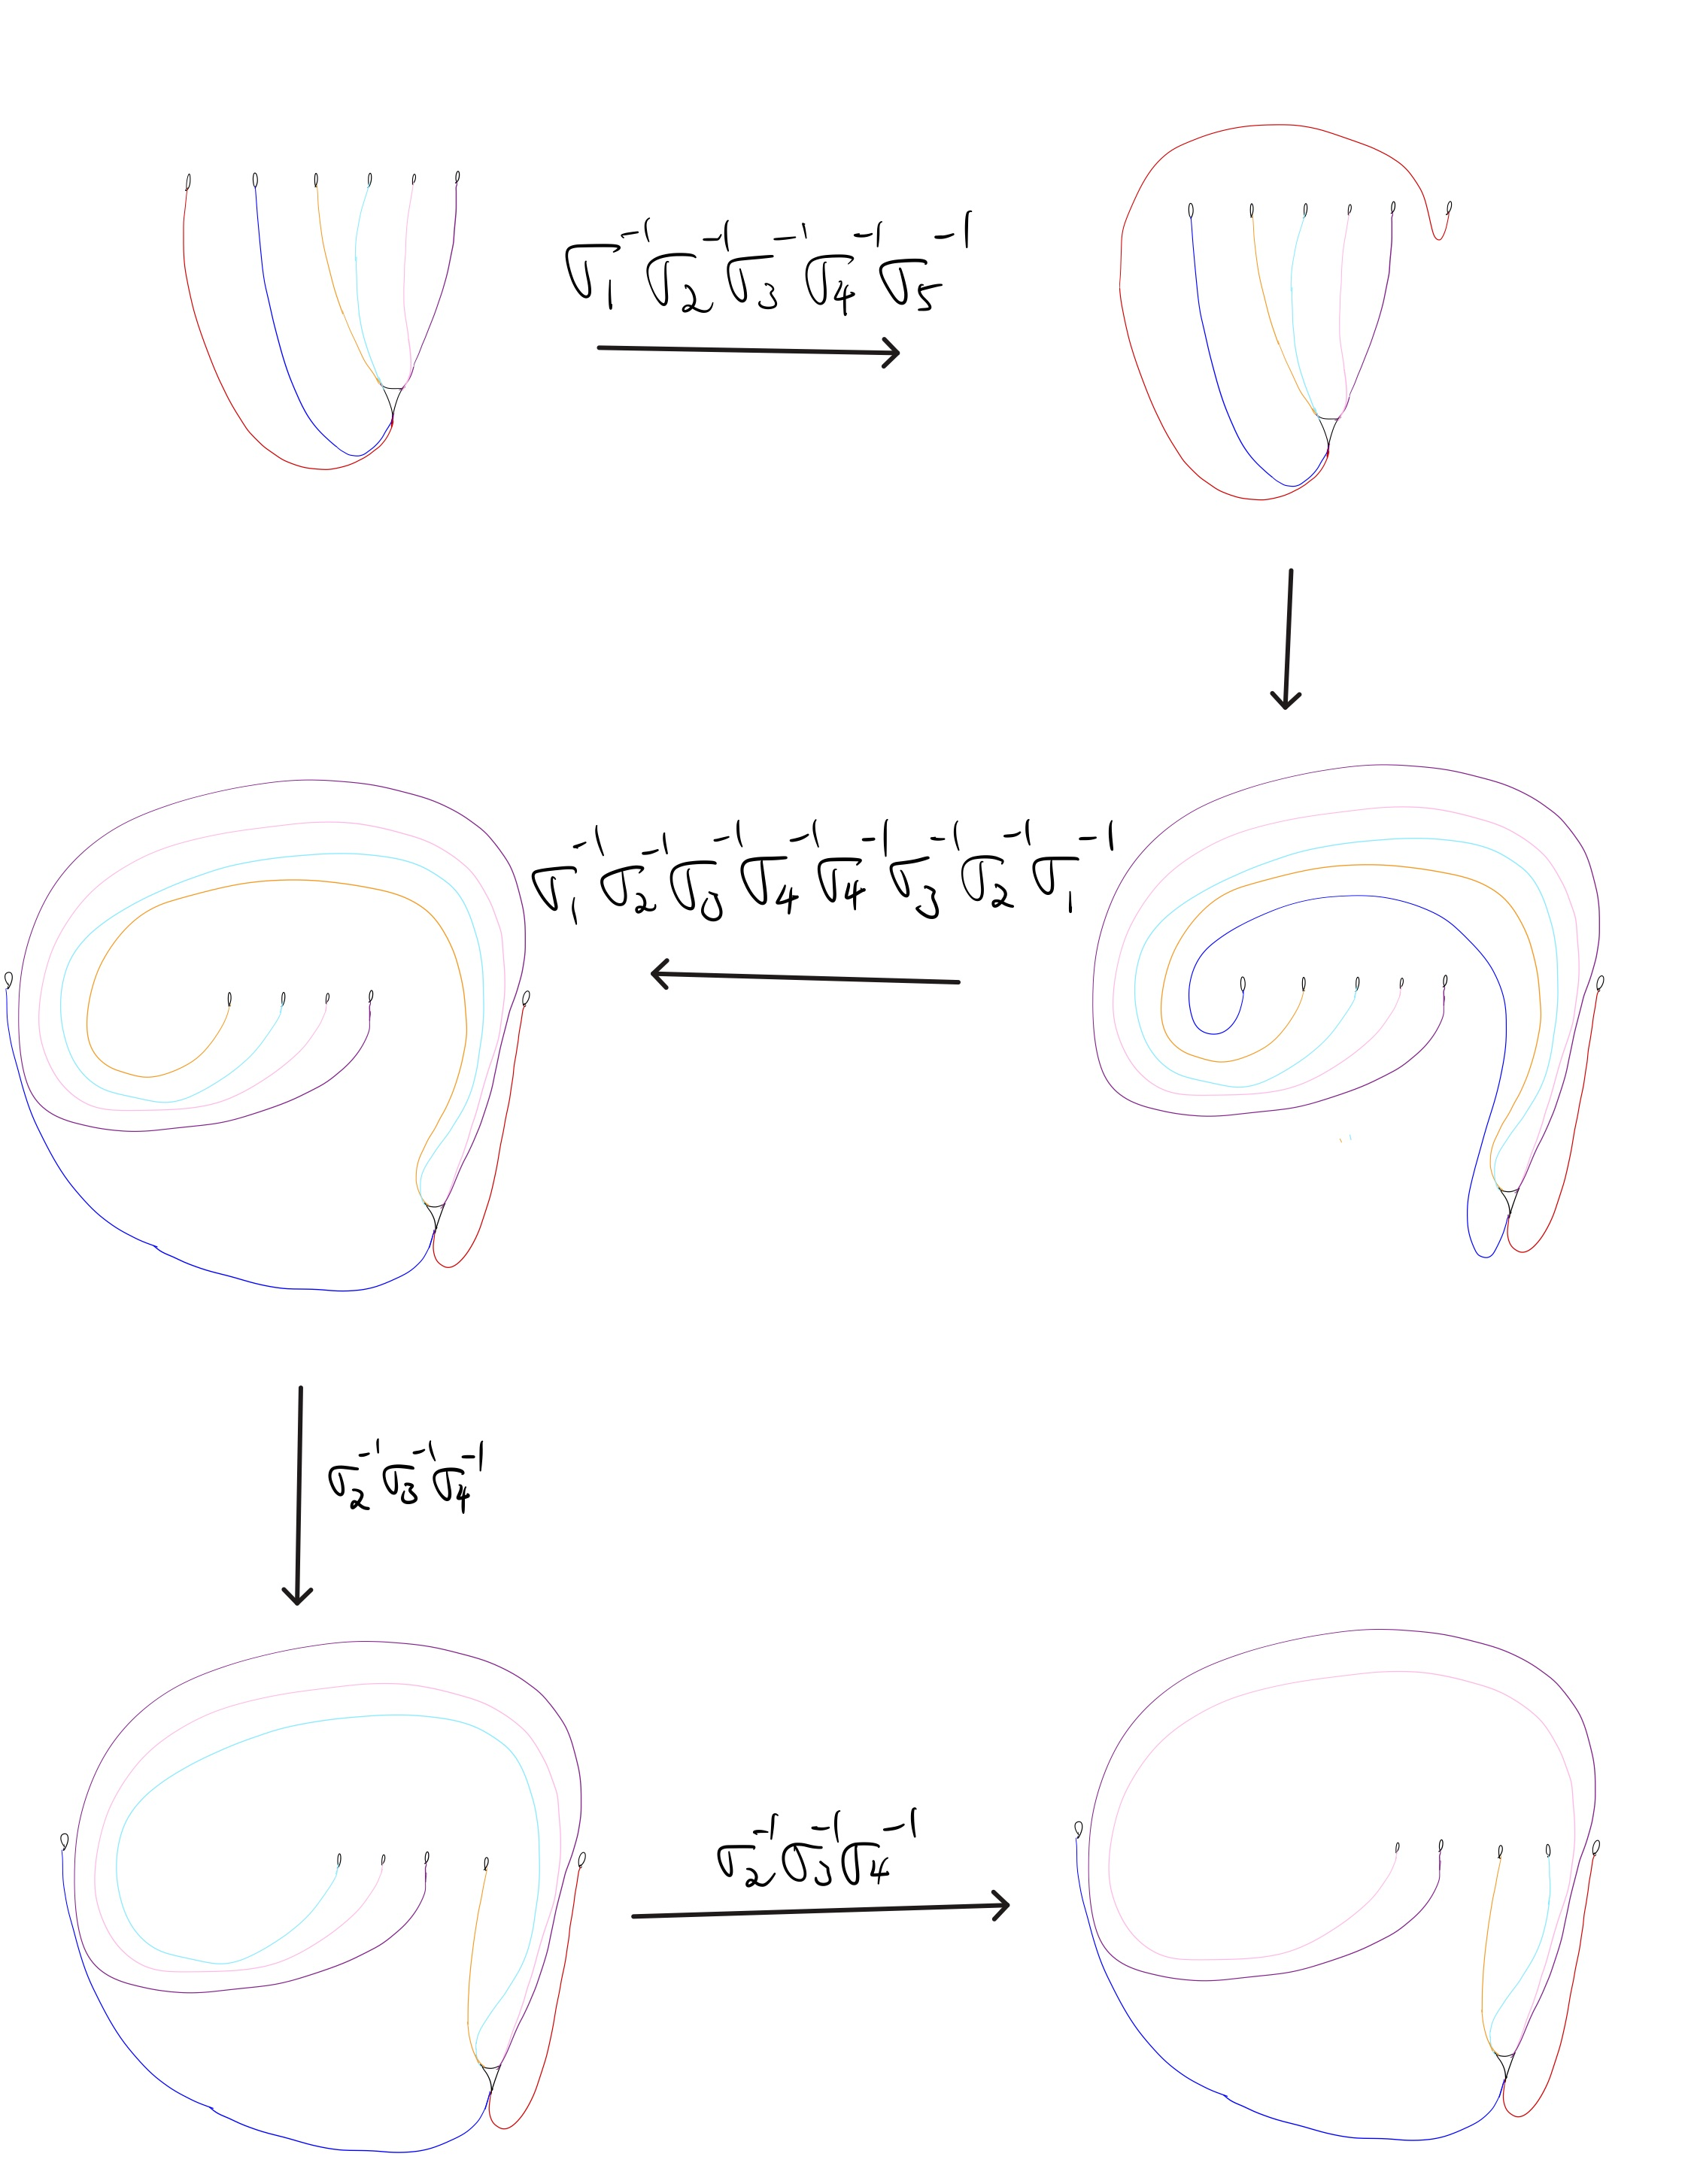
\includegraphics[width=\linewidth, height=0.45\textheight, keepaspectratio]{figures_braid/figures_candelabra/H-1.jpg}\\
    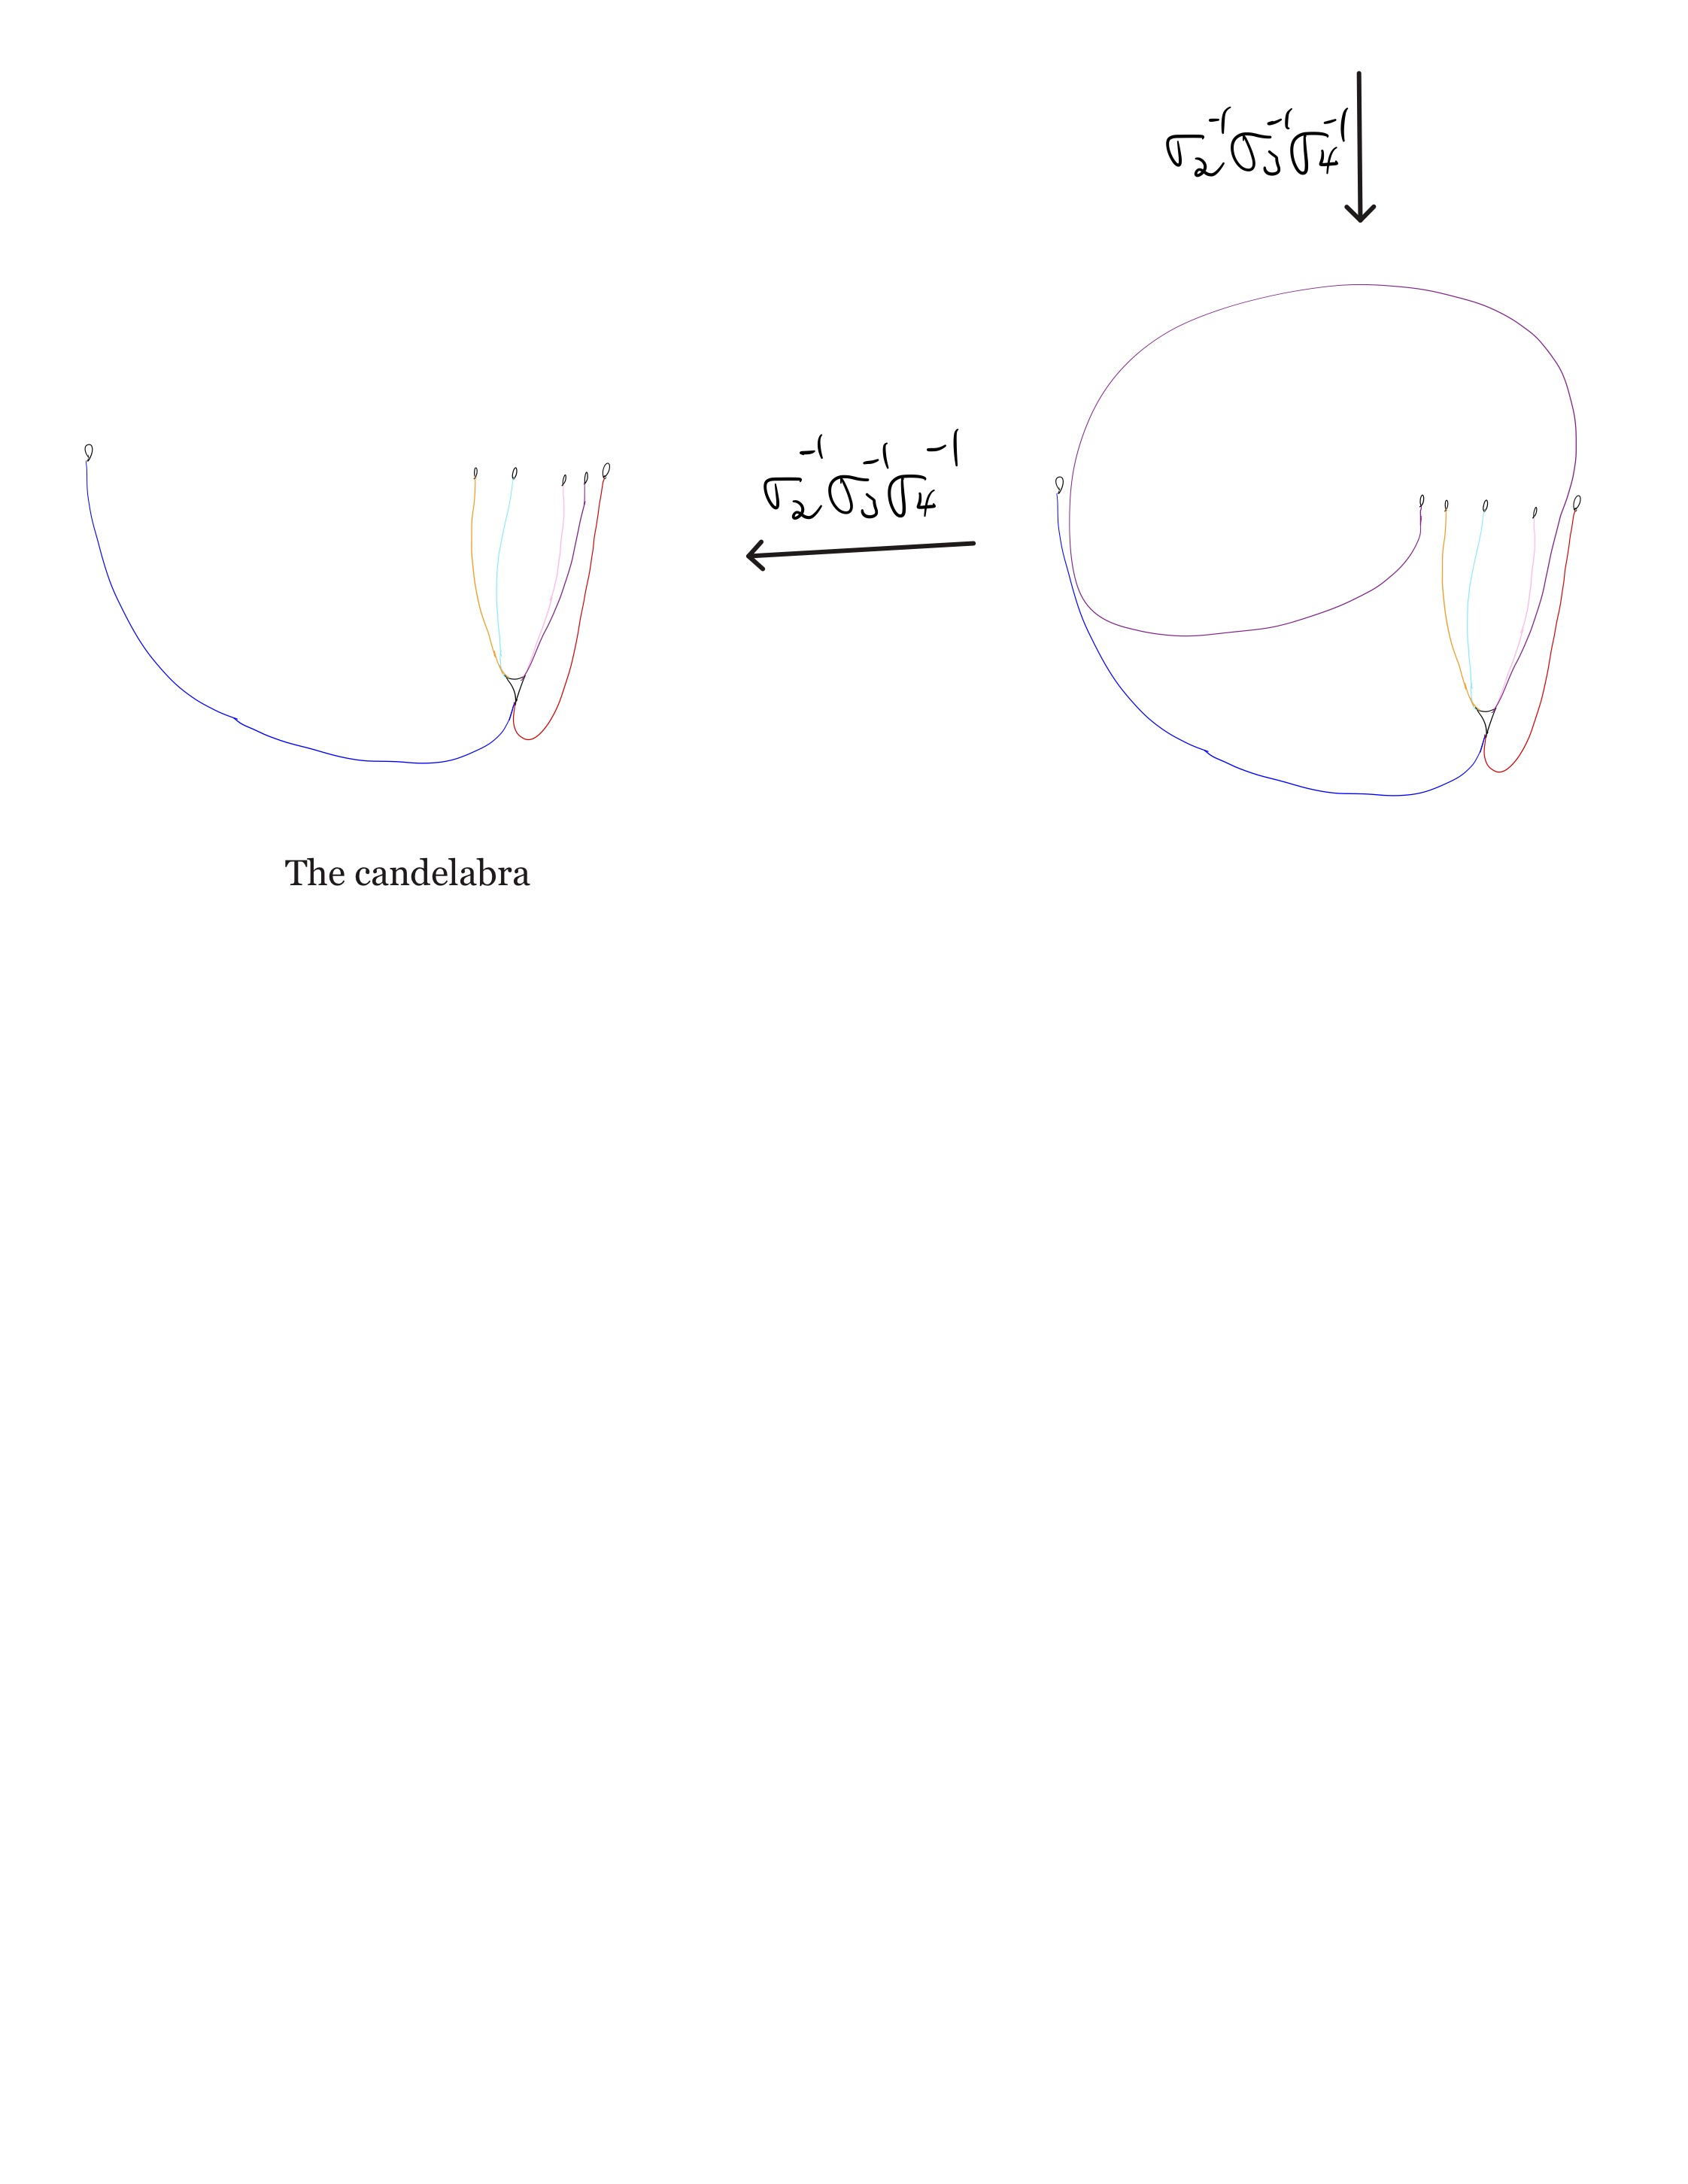
\includegraphics[width=\linewidth, height=0.45\textheight, keepaspectratio]{figures_braid/figures_candelabra/H-2.jpg}
    \caption{This sequence shows the inverse of the braid $H$ can be thought of as swinging the right-most arm of the Candelabra all the way to the left.}
    \label{fig:candelabra_braid_H_main}
\end{figure*}

\clearpage

\section{Candidate 1}\label{sec:braid G}
The inverse of the following braid, which we call $G$, carries Candidate Train Track Map 1 of the Candelabra train track:

\begin{flushleft}
$\displaystyle G = \allowbreak\sigma_{3}^{-1}\allowbreak\sigma_{4}^{-1}\allowbreak\sigma_{2}^{-1}\allowbreak\sigma_{3}^{-1}\allowbreak\sigma_{1}^{-1}\allowbreak\sigma_{2}^{-1}\allowbreak\sigma_{3}^{-1}\allowbreak\sigma_{4}^{-1}\allowbreak\sigma_{3}\allowbreak\sigma_{4}^{-1}\allowbreak\sigma_{5}^{-1}\allowbreak\sigma_{4}^{-1}\allowbreak\sigma_{3}^{-1}\allowbreak\sigma_{4}\allowbreak\sigma_{5}\allowbreak\sigma_{2}^{-1}\allowbreak\sigma_{1}^{-1}\allowbreak\sigma_{1}^{-1}\allowbreak\sigma_{2}^{-1}\allowbreak\sigma_{1}^{-1}\allowbreak\sigma_{1}^{-1} \cdot \allowbreak\sigma_{5}\allowbreak\sigma_{4}\allowbreak\sigma_{3}\allowbreak\sigma_{2}\allowbreak\sigma_{1}\allowbreak\sigma_{2}\allowbreak\sigma_{3}\allowbreak\sigma_{4}\allowbreak\sigma_{5}\allowbreak\sigma_{5}\allowbreak\sigma_{4}\allowbreak\sigma_{3}\allowbreak\sigma_{2}\allowbreak\sigma_{3}\allowbreak\sigma_{4}\allowbreak\sigma_{5}\allowbreak\sigma_{5}\allowbreak\sigma_{4}\allowbreak\sigma_{3}\allowbreak\sigma_{4}\allowbreak\sigma_{5}\allowbreak\sigma_{5}\allowbreak\sigma_{4}\allowbreak\sigma_{5}\allowbreak\sigma_{5}$
\end{flushleft}

This is shown in Figure \ref{fig:candelabra_braid_G}.

\begin{figure*}[p]
    \centering
    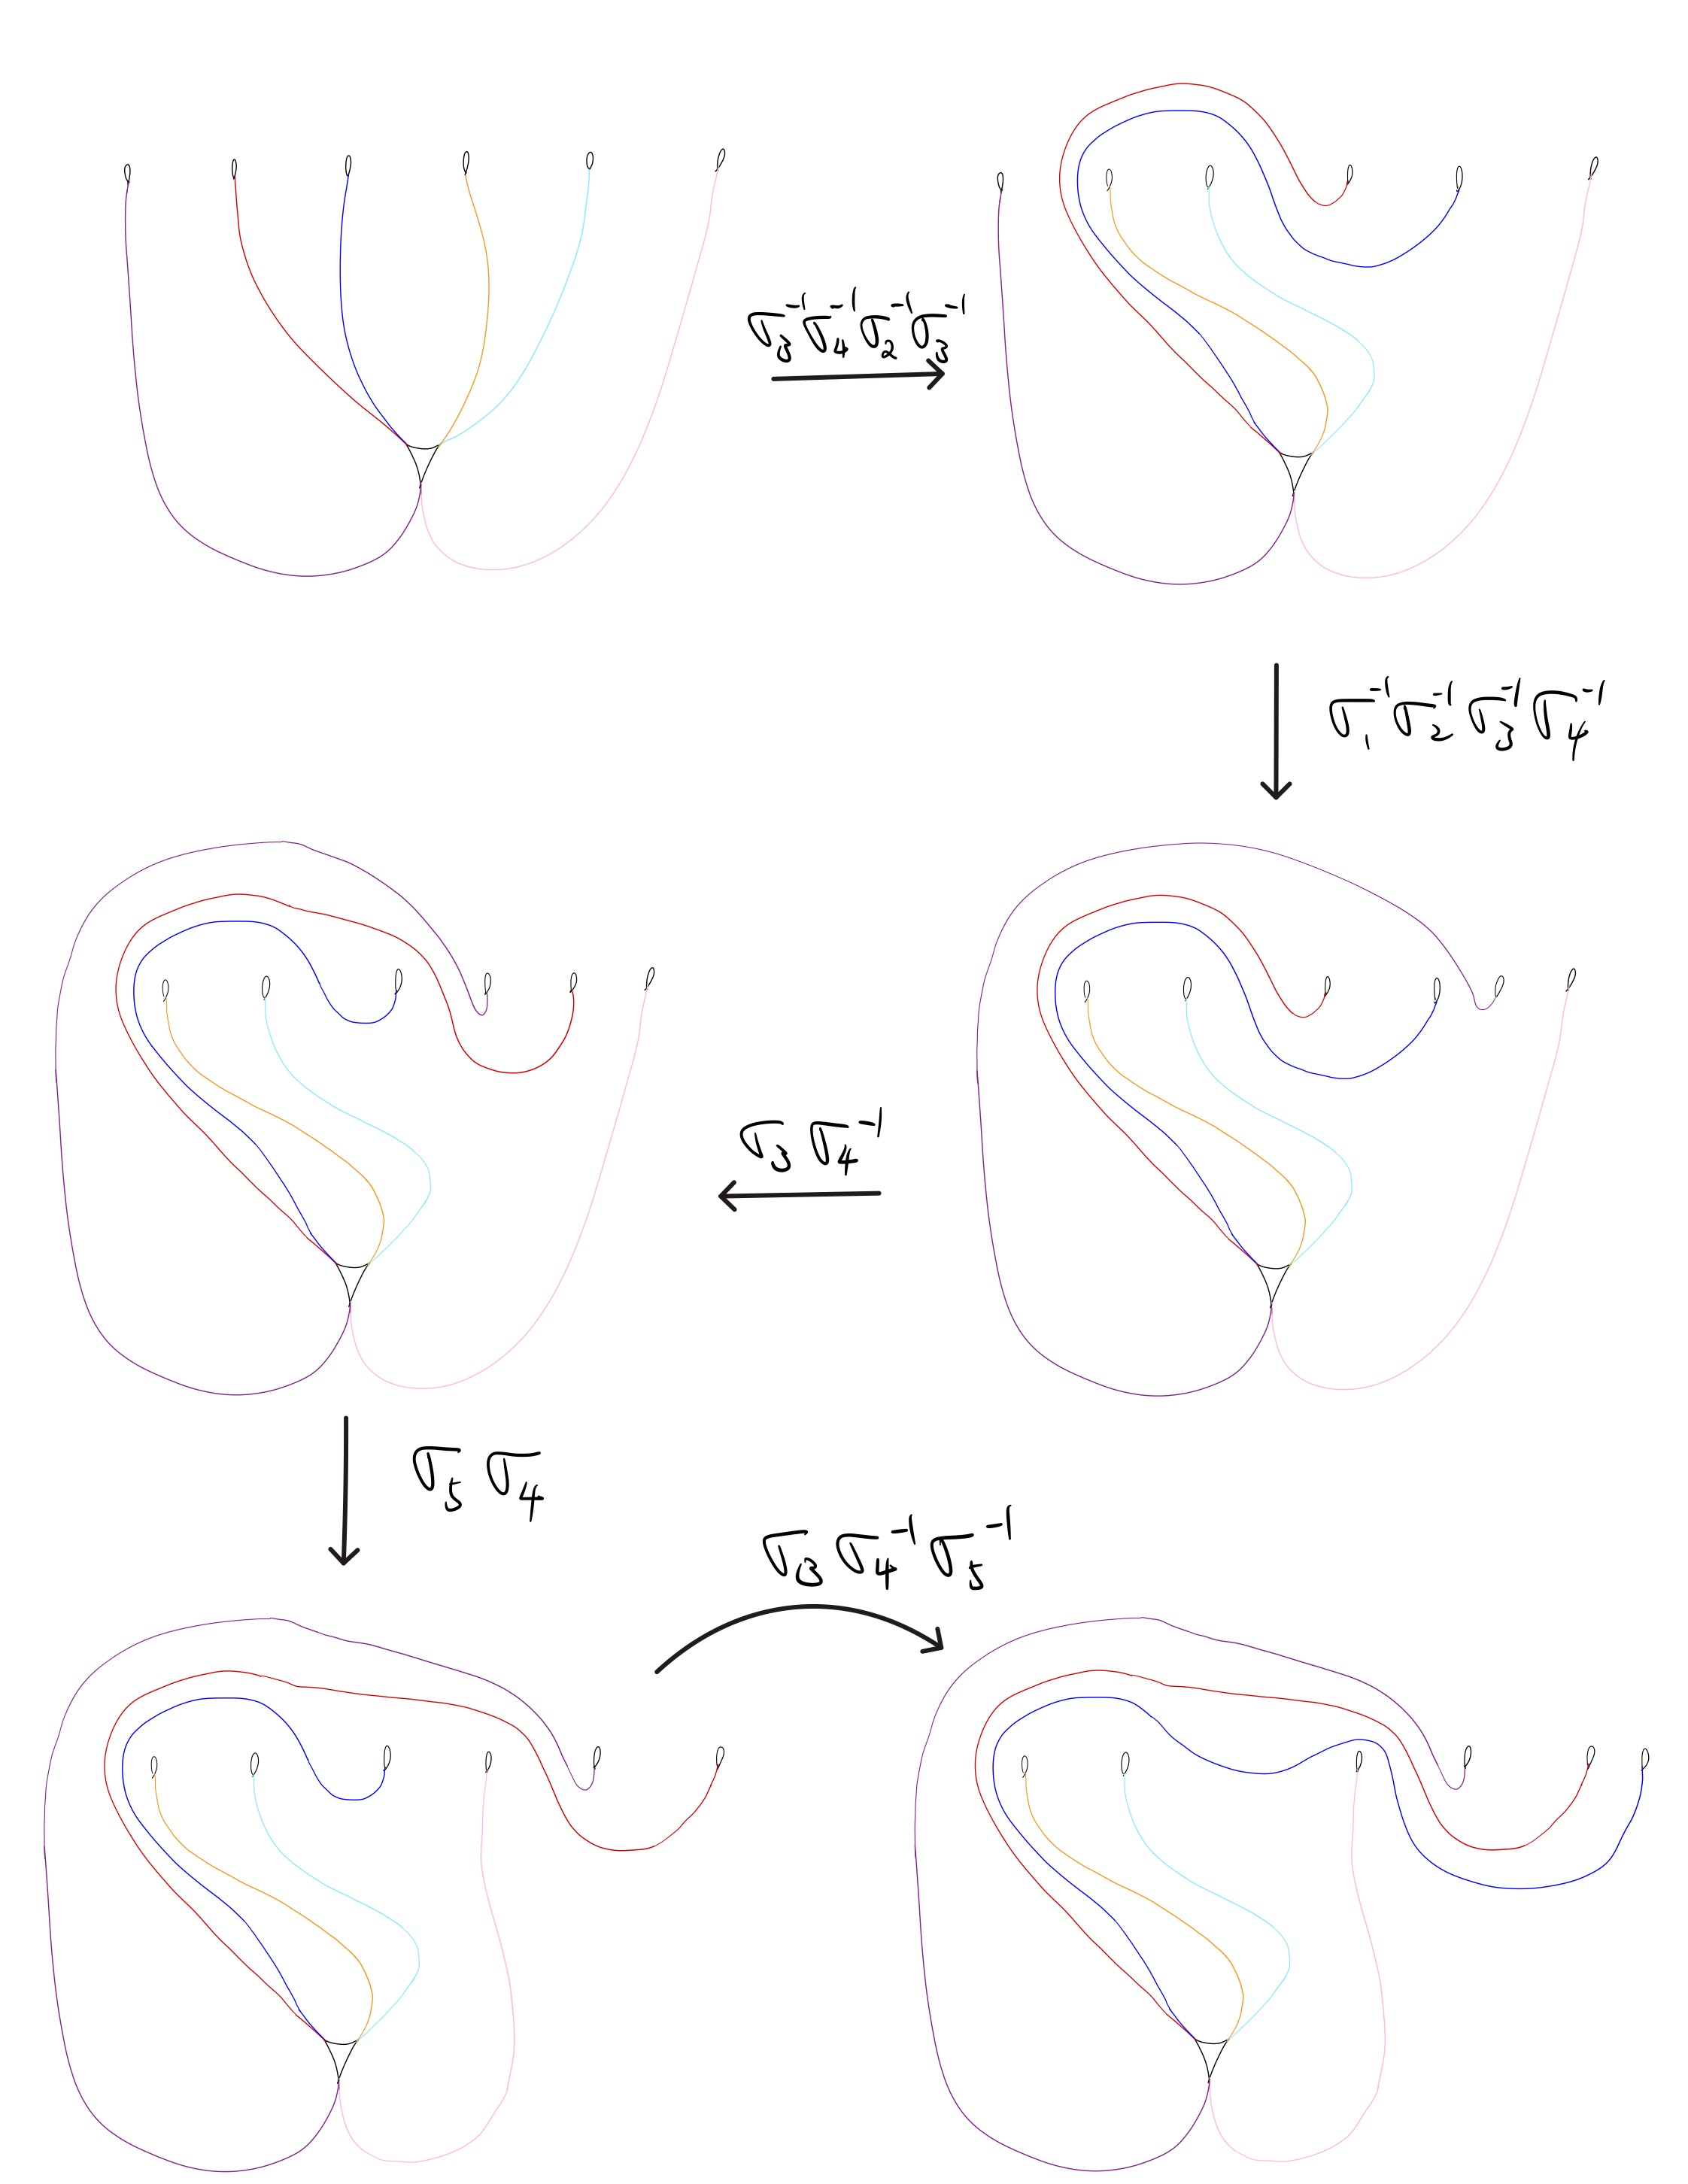
\includegraphics[width=\linewidth, height=0.45\textheight, keepaspectratio]{figures_braid/figures_candelabra/Candelabra Braid 1 NHT-2.jpg}\\
    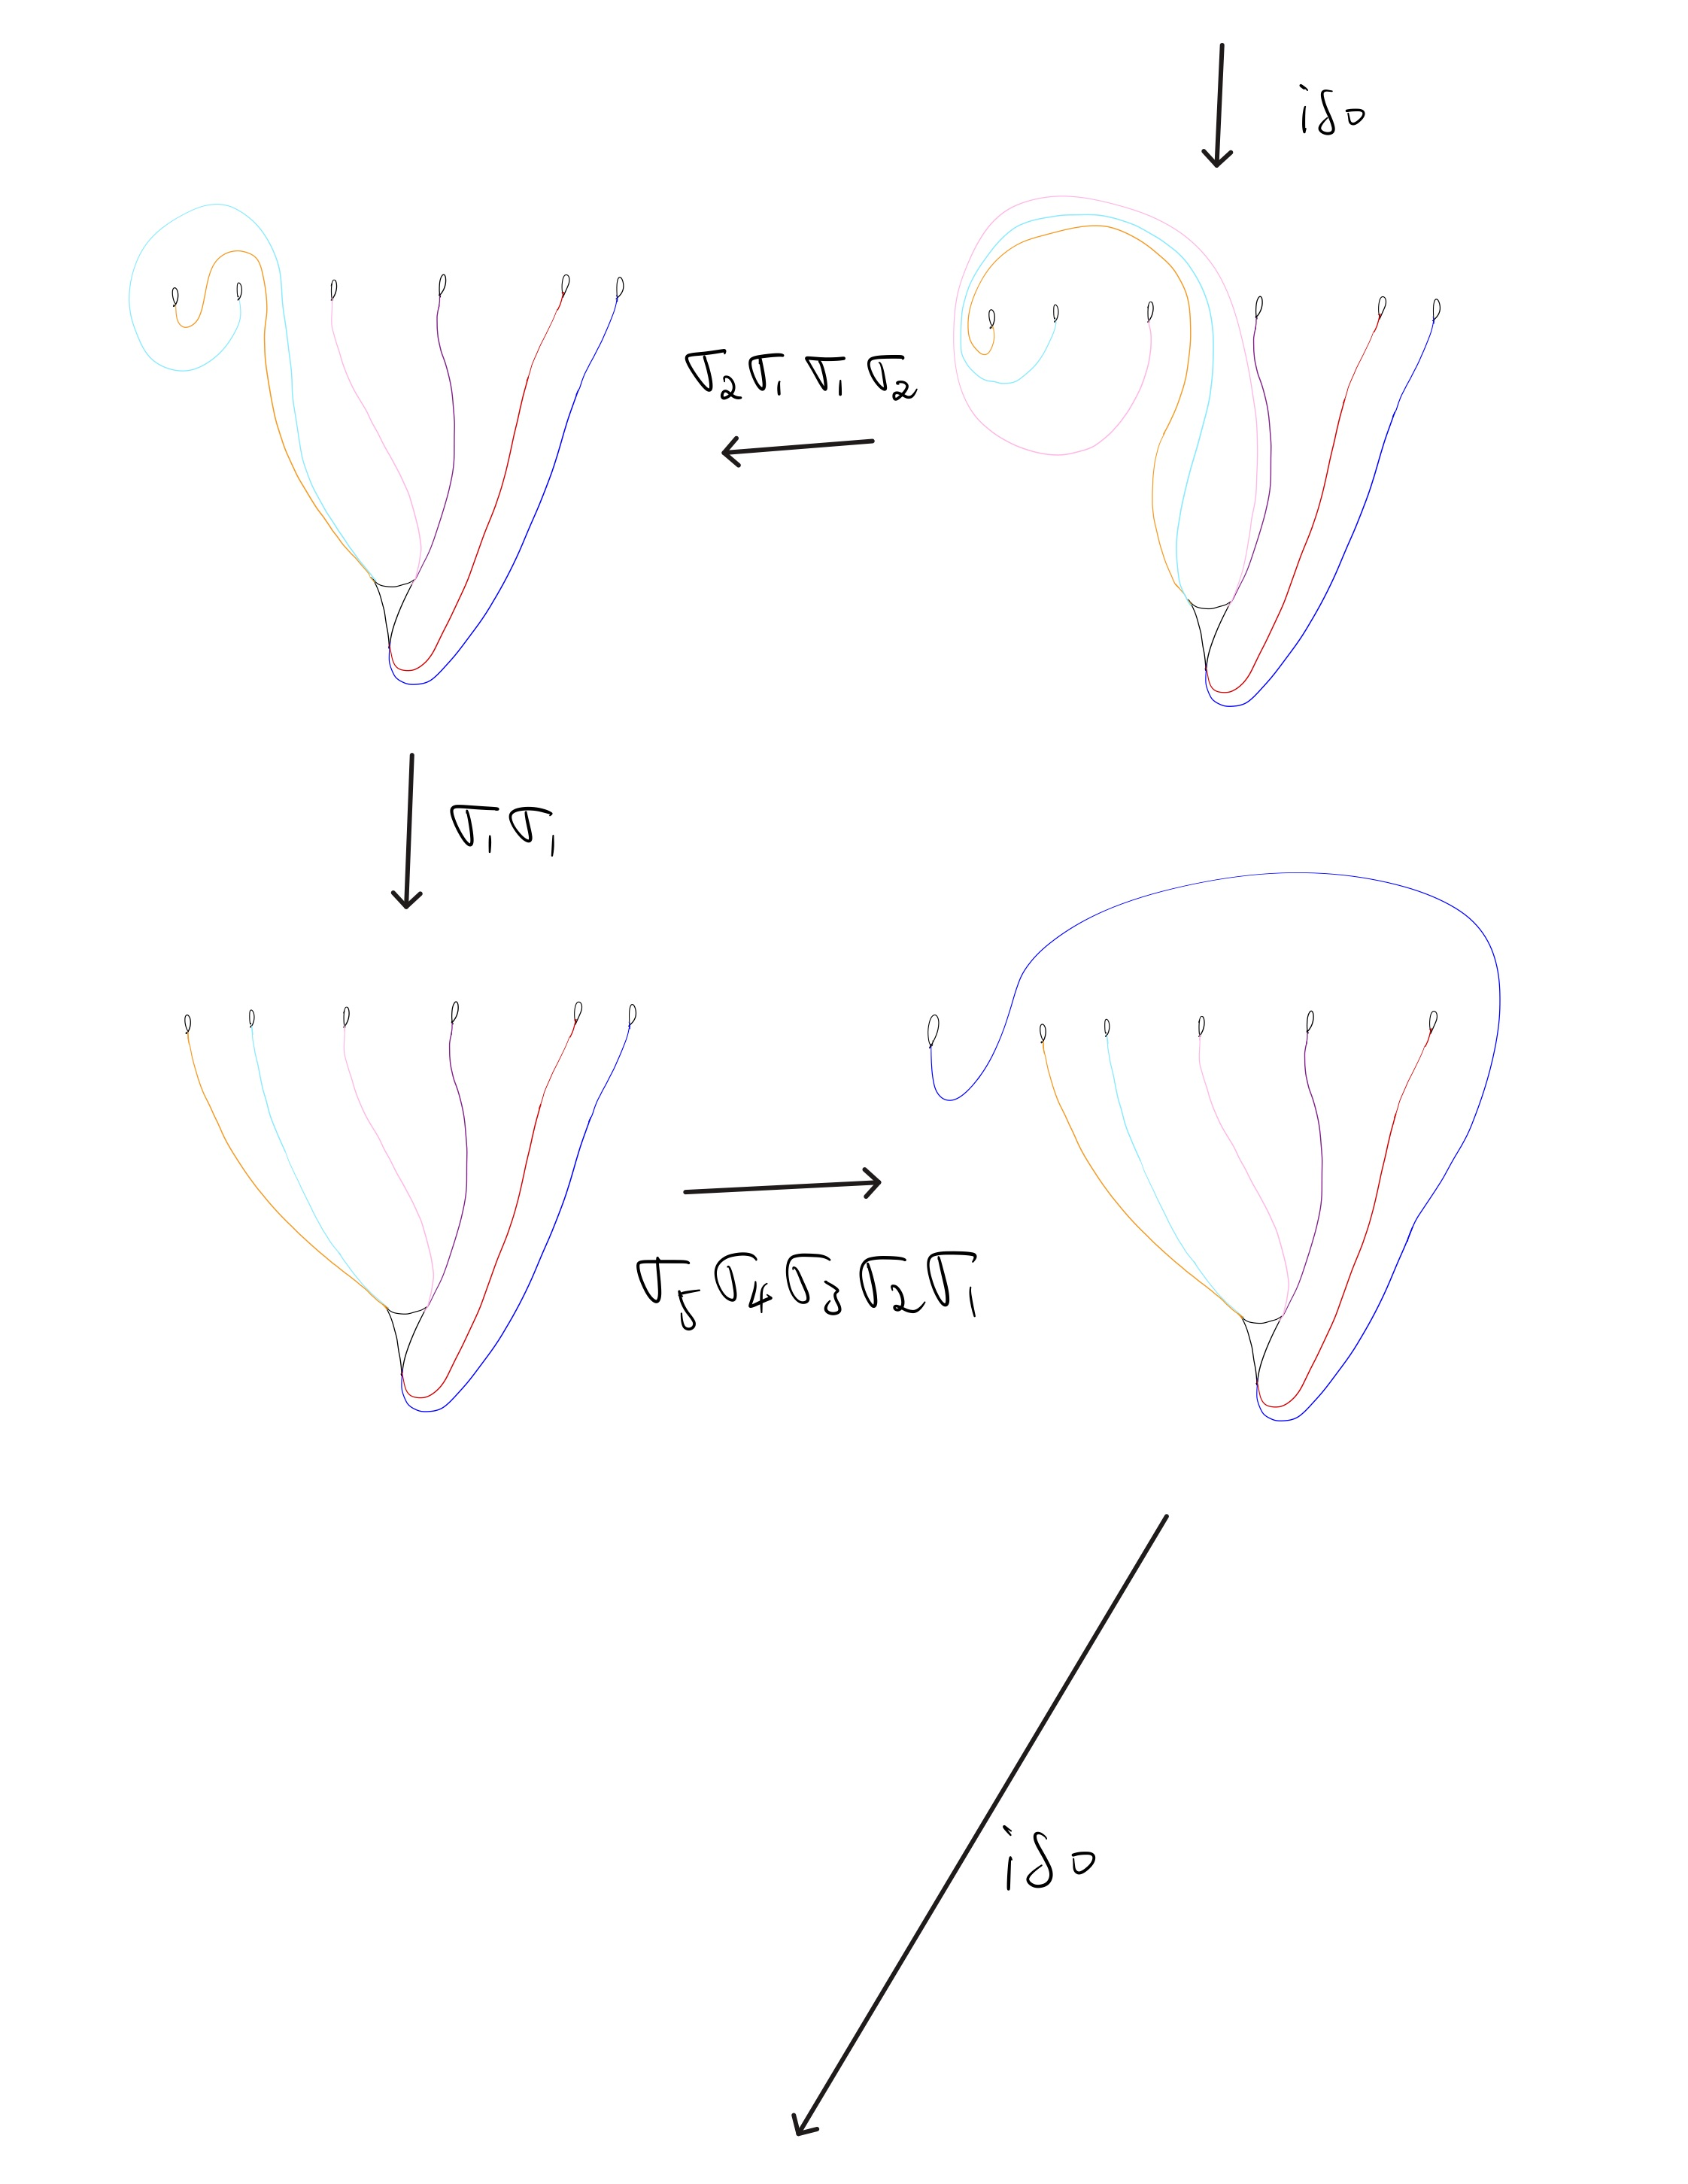
\includegraphics[width=\linewidth, height=0.45\textheight, keepaspectratio]{figures_braid/figures_candelabra/Candelabra Braid 1 NHT-3.jpg}
    \caption{This sequence shows the inverse of the braid $G$ carries Train Track Candidate 1.}
    \label{fig:candelabra_braid_G}
\end{figure*}

\begin{figure*}[p]
    \ContinuedFloat
    \centering
    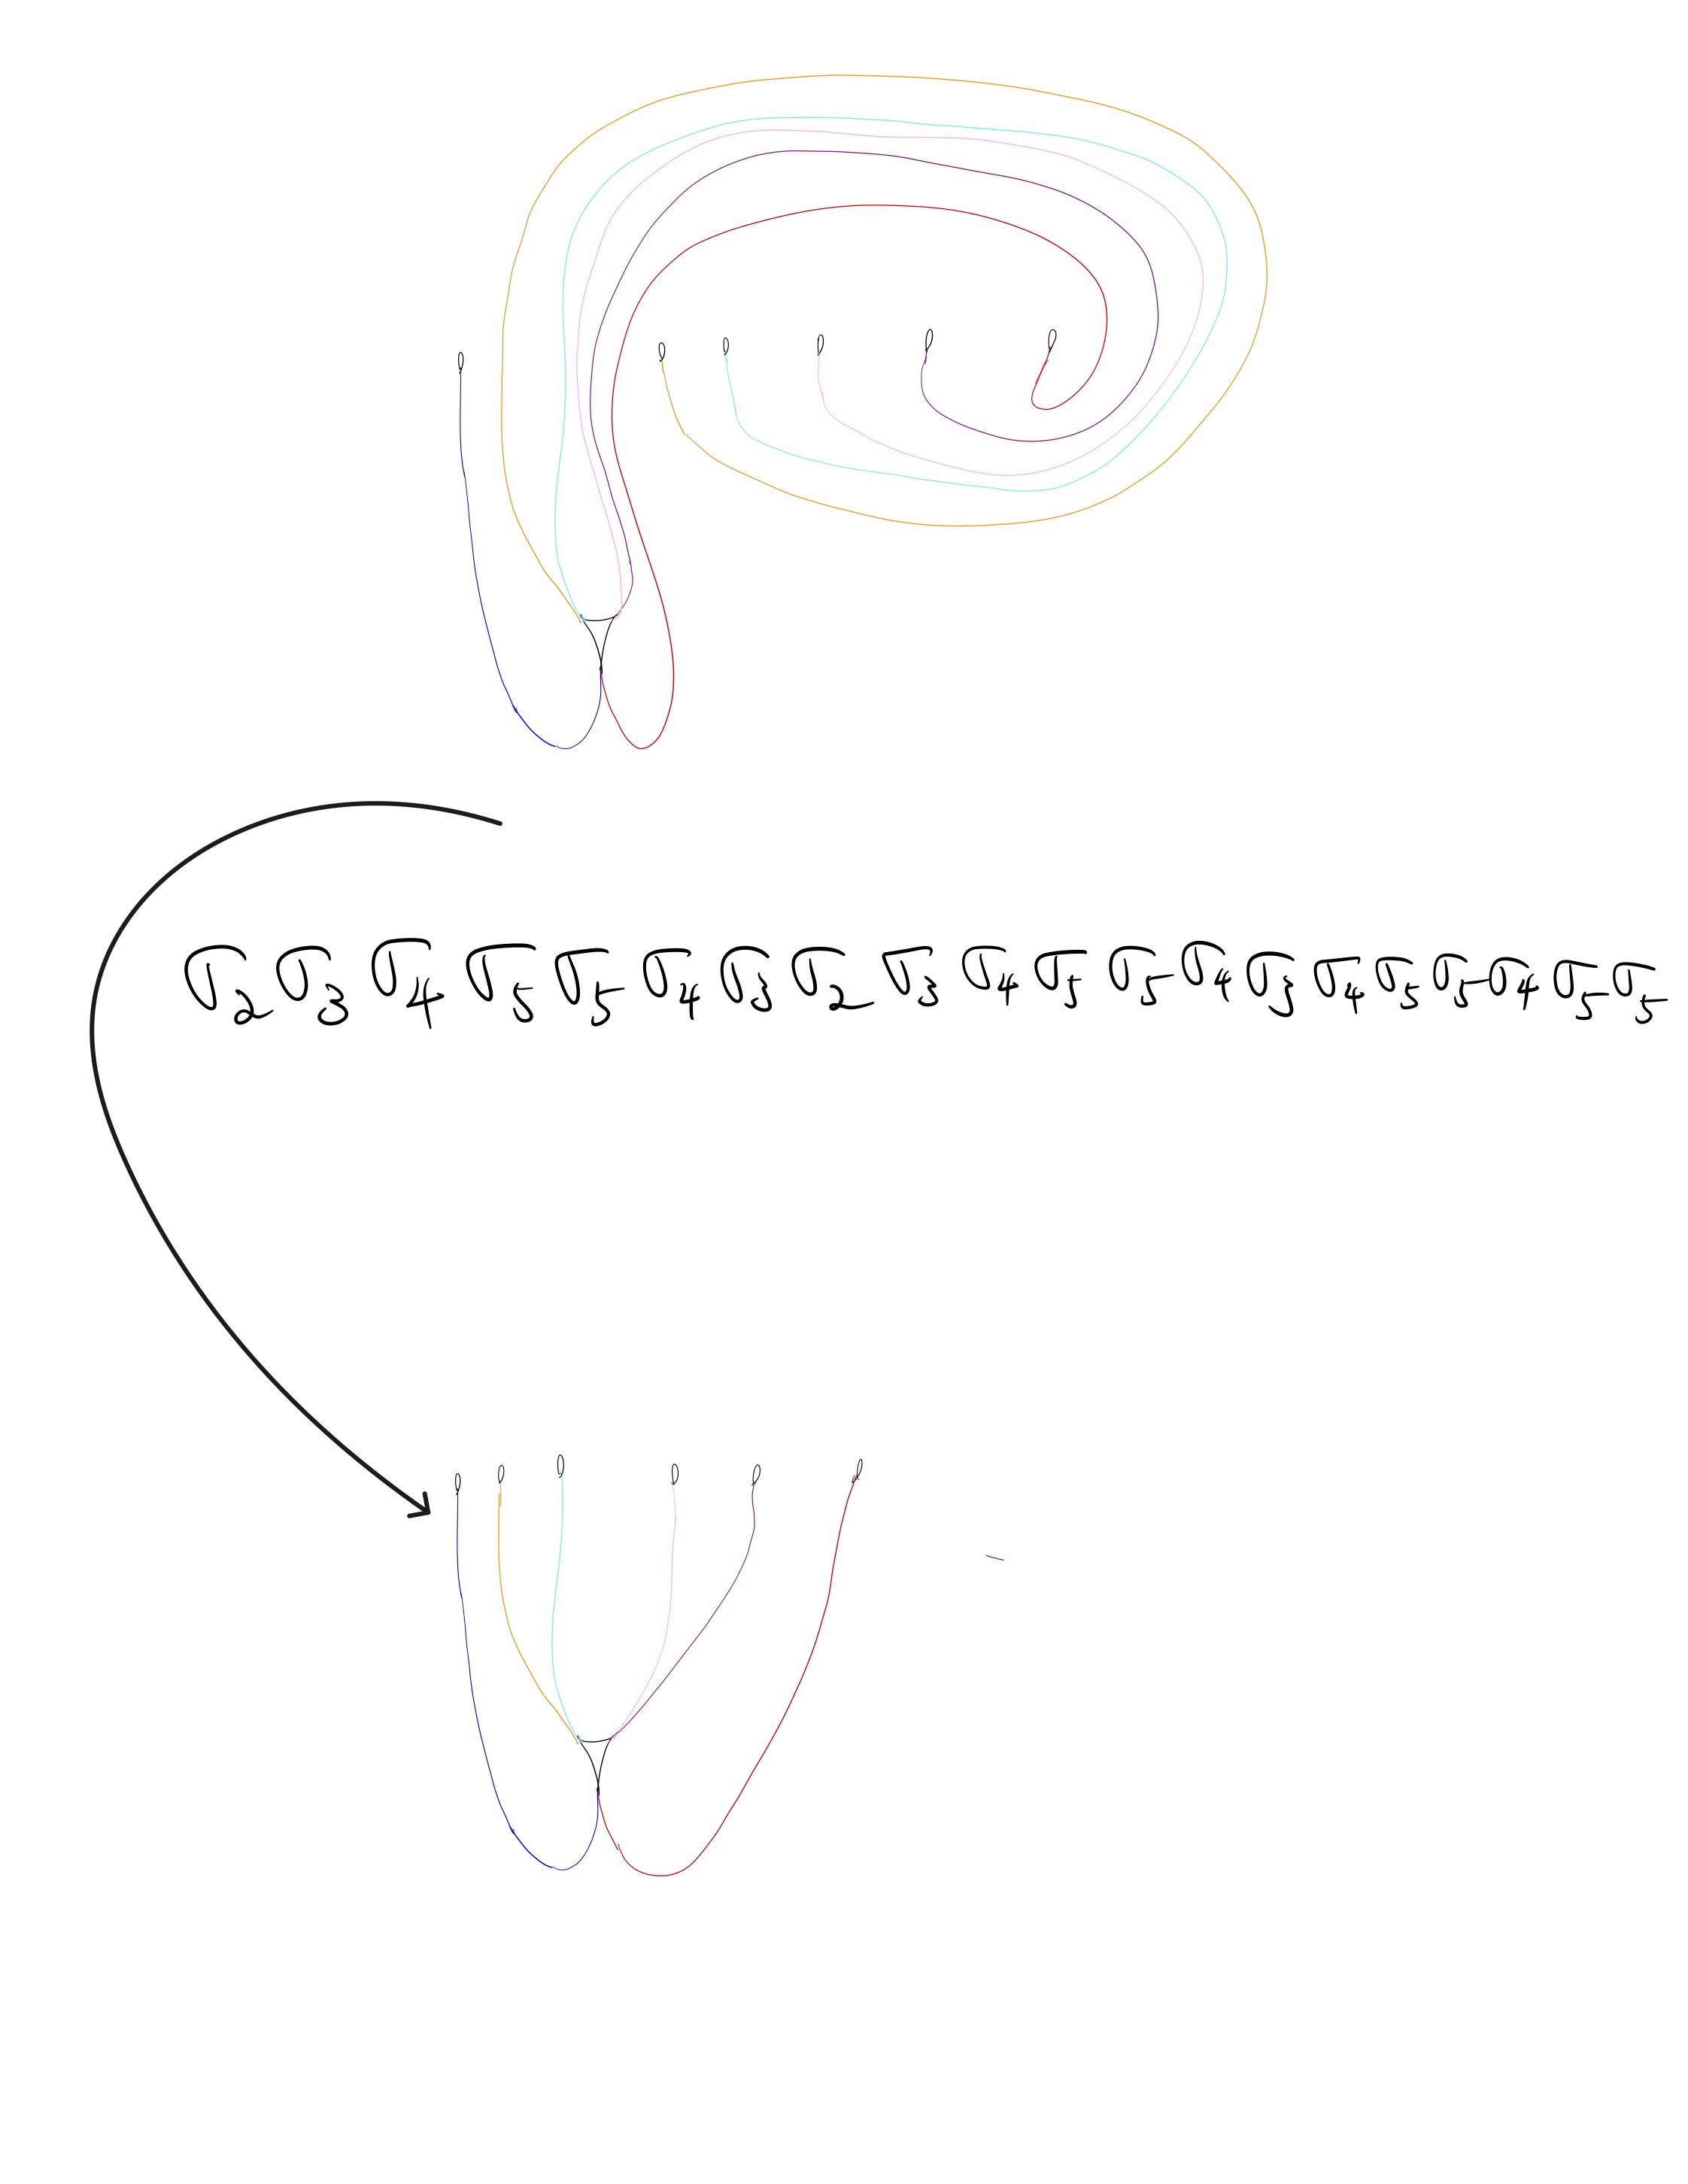
\includegraphics[width=\linewidth, height=0.45\textheight, keepaspectratio]{figures_braid/figures_candelabra/Candelabra Braid 1 NHT-4.jpg}
    \caption[]{This sequence shows the inverse of the braid $G$ carries Train Track Candidate 1 (continued).}
\end{figure*}

\clearpage

\section{Candidate 2}
Train Track Map Candidate Family 2 of the Candelabra train track is shown in Figure \ref{fig:candelabra_braid_b2_map}. Note there is twisting between $\fbr$ and $\fbb$. See \ref{Jehu} for details.

\begin{figure*}[ht]
    \centering
    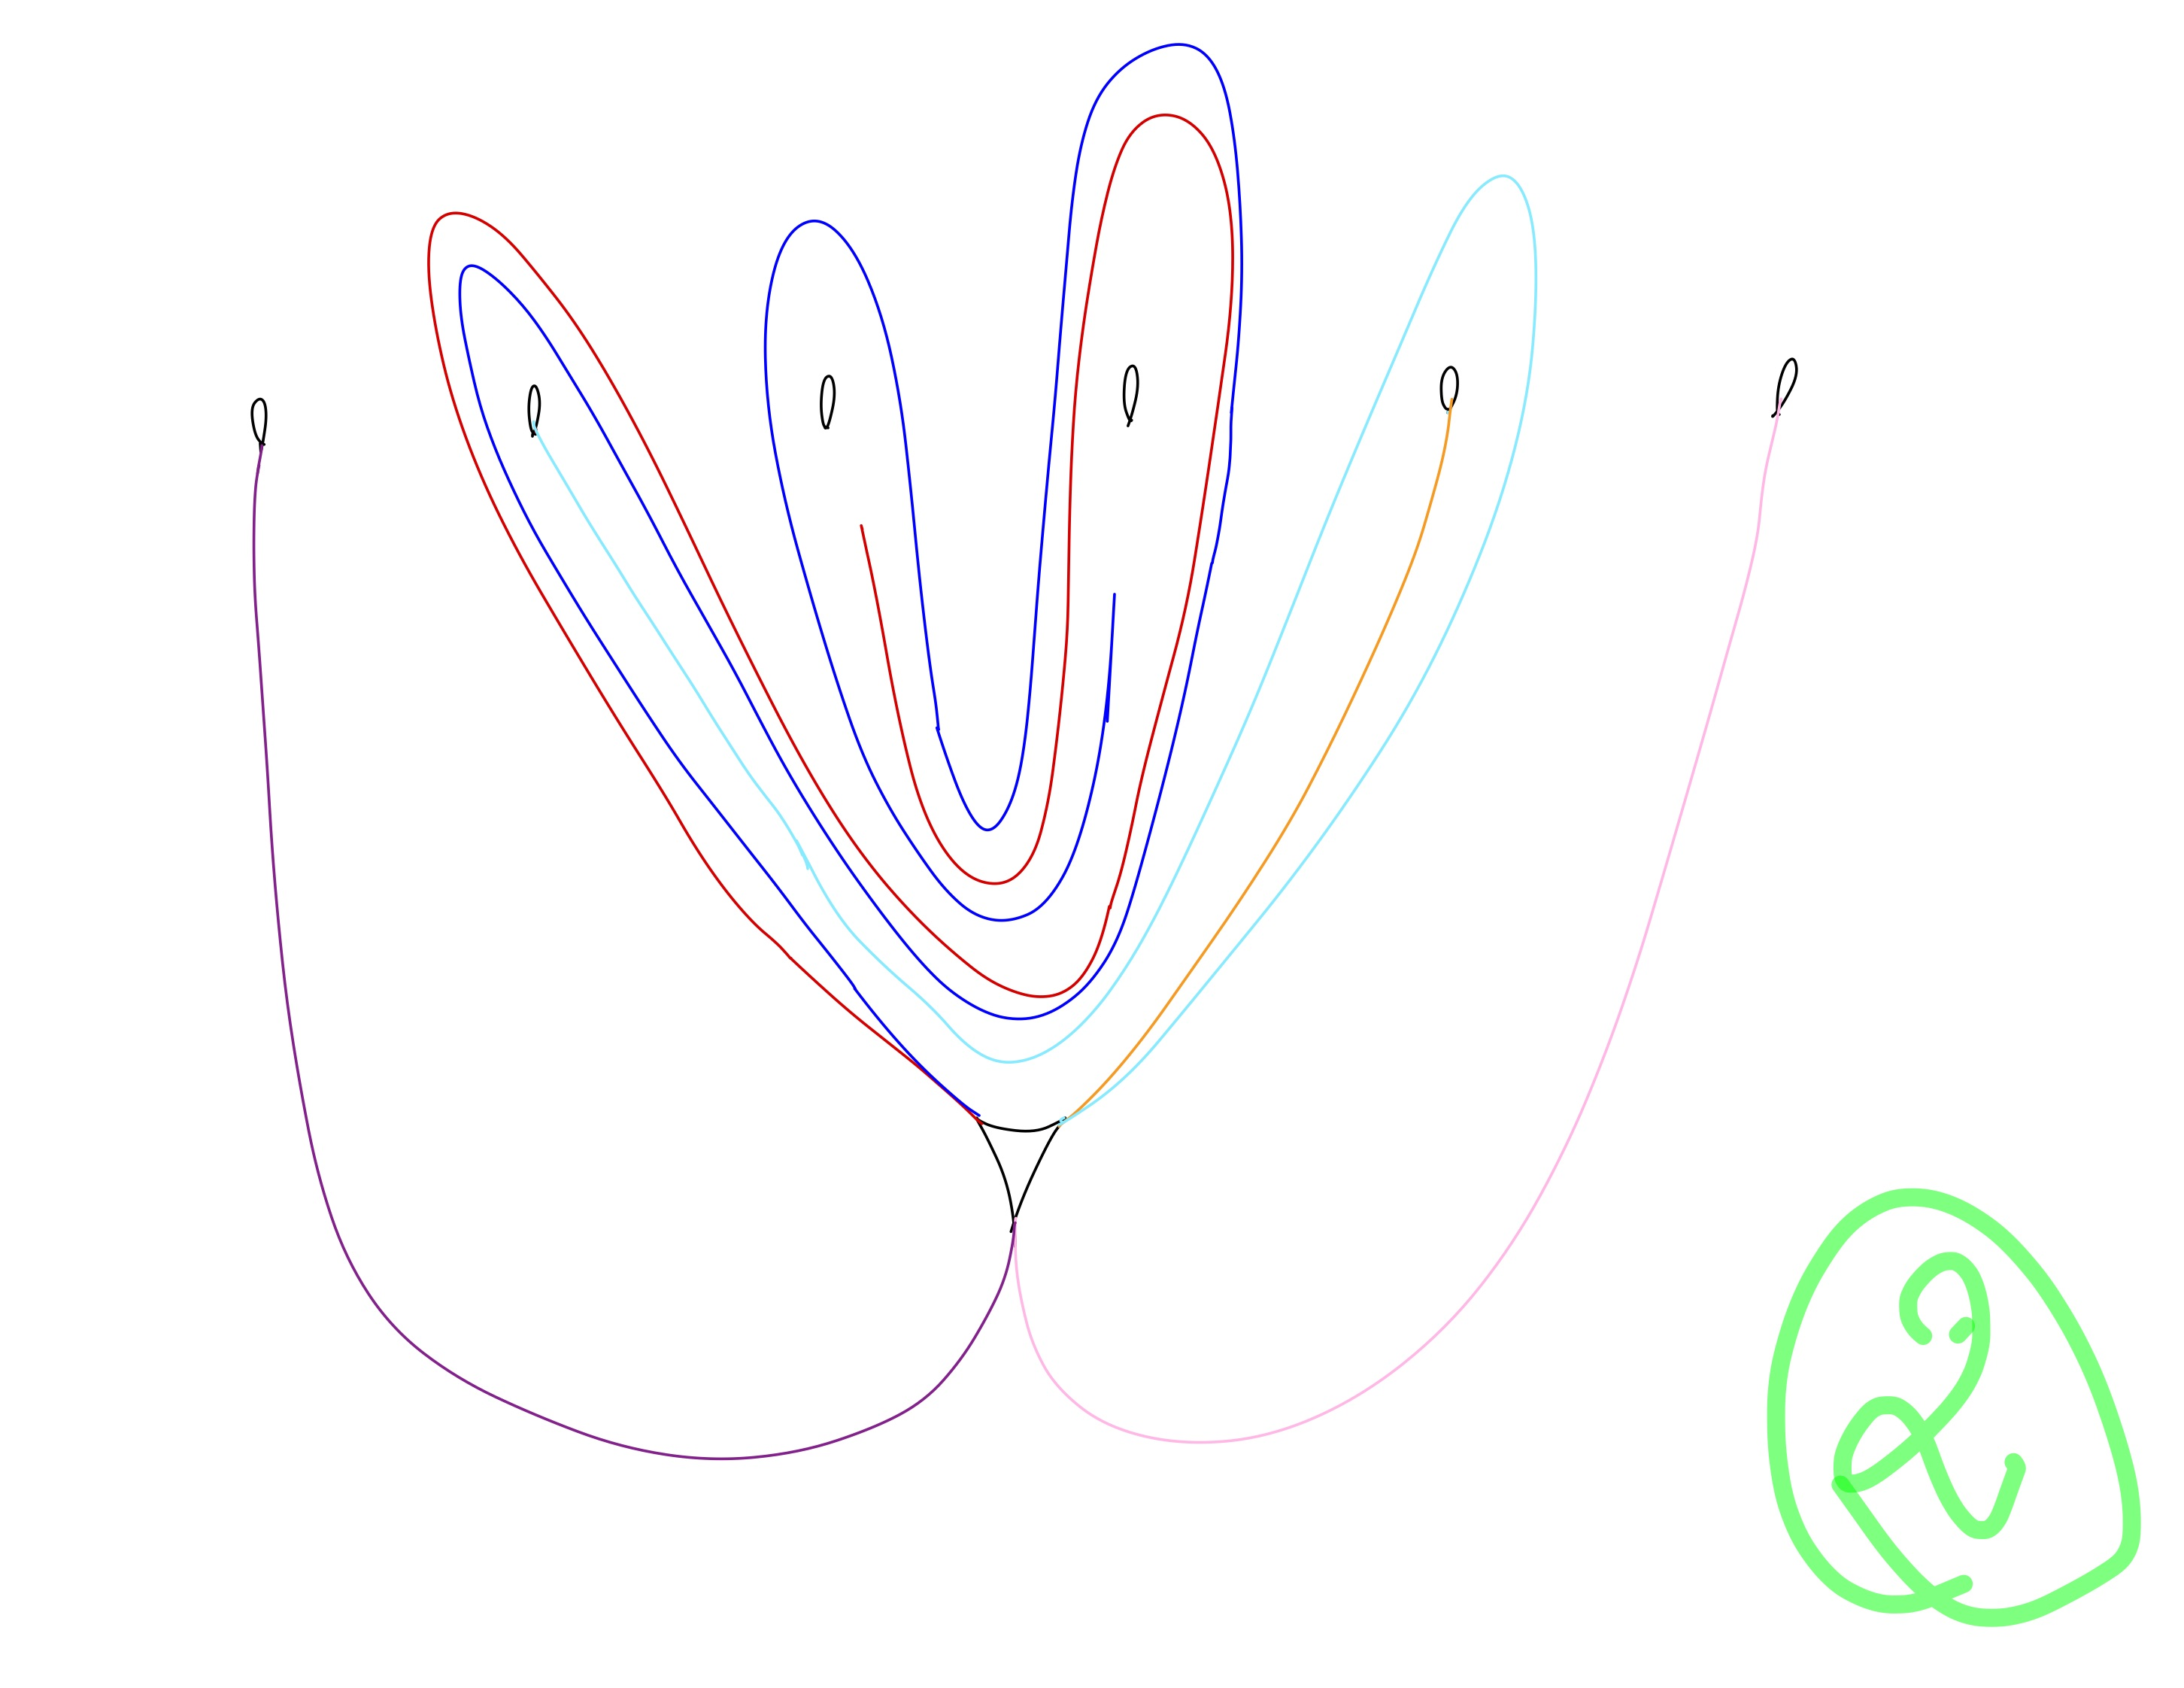
\includegraphics[width=\linewidth, height=0.45\textheight, keepaspectratio]{figures_braid/figures_candelabra/Candelabra Braid 2 Jehu-1.jpg}
    \caption{Train Track Map Candidate Family 2 of the Candelabra.}
    \label{fig:candelabra_braid_b2_map}
\end{figure*}

The inverse of the following braid, which we call $G$, carries this family of train track maps:
\[
b_2^c = \sigma_4^k\sigma_2^{-1}\sigma_3^{-1}\sigma_4 \circ G
\]
where $G$ is the braid of Section \ref{sec:braid G}, and $k\geq 1$ ($k\in \mathbb{Z}$) is the twisting parameter. This is shown in Figure \ref{fig:candelabra_braid_b2}.

\begin{figure*}[p]
    \centering
    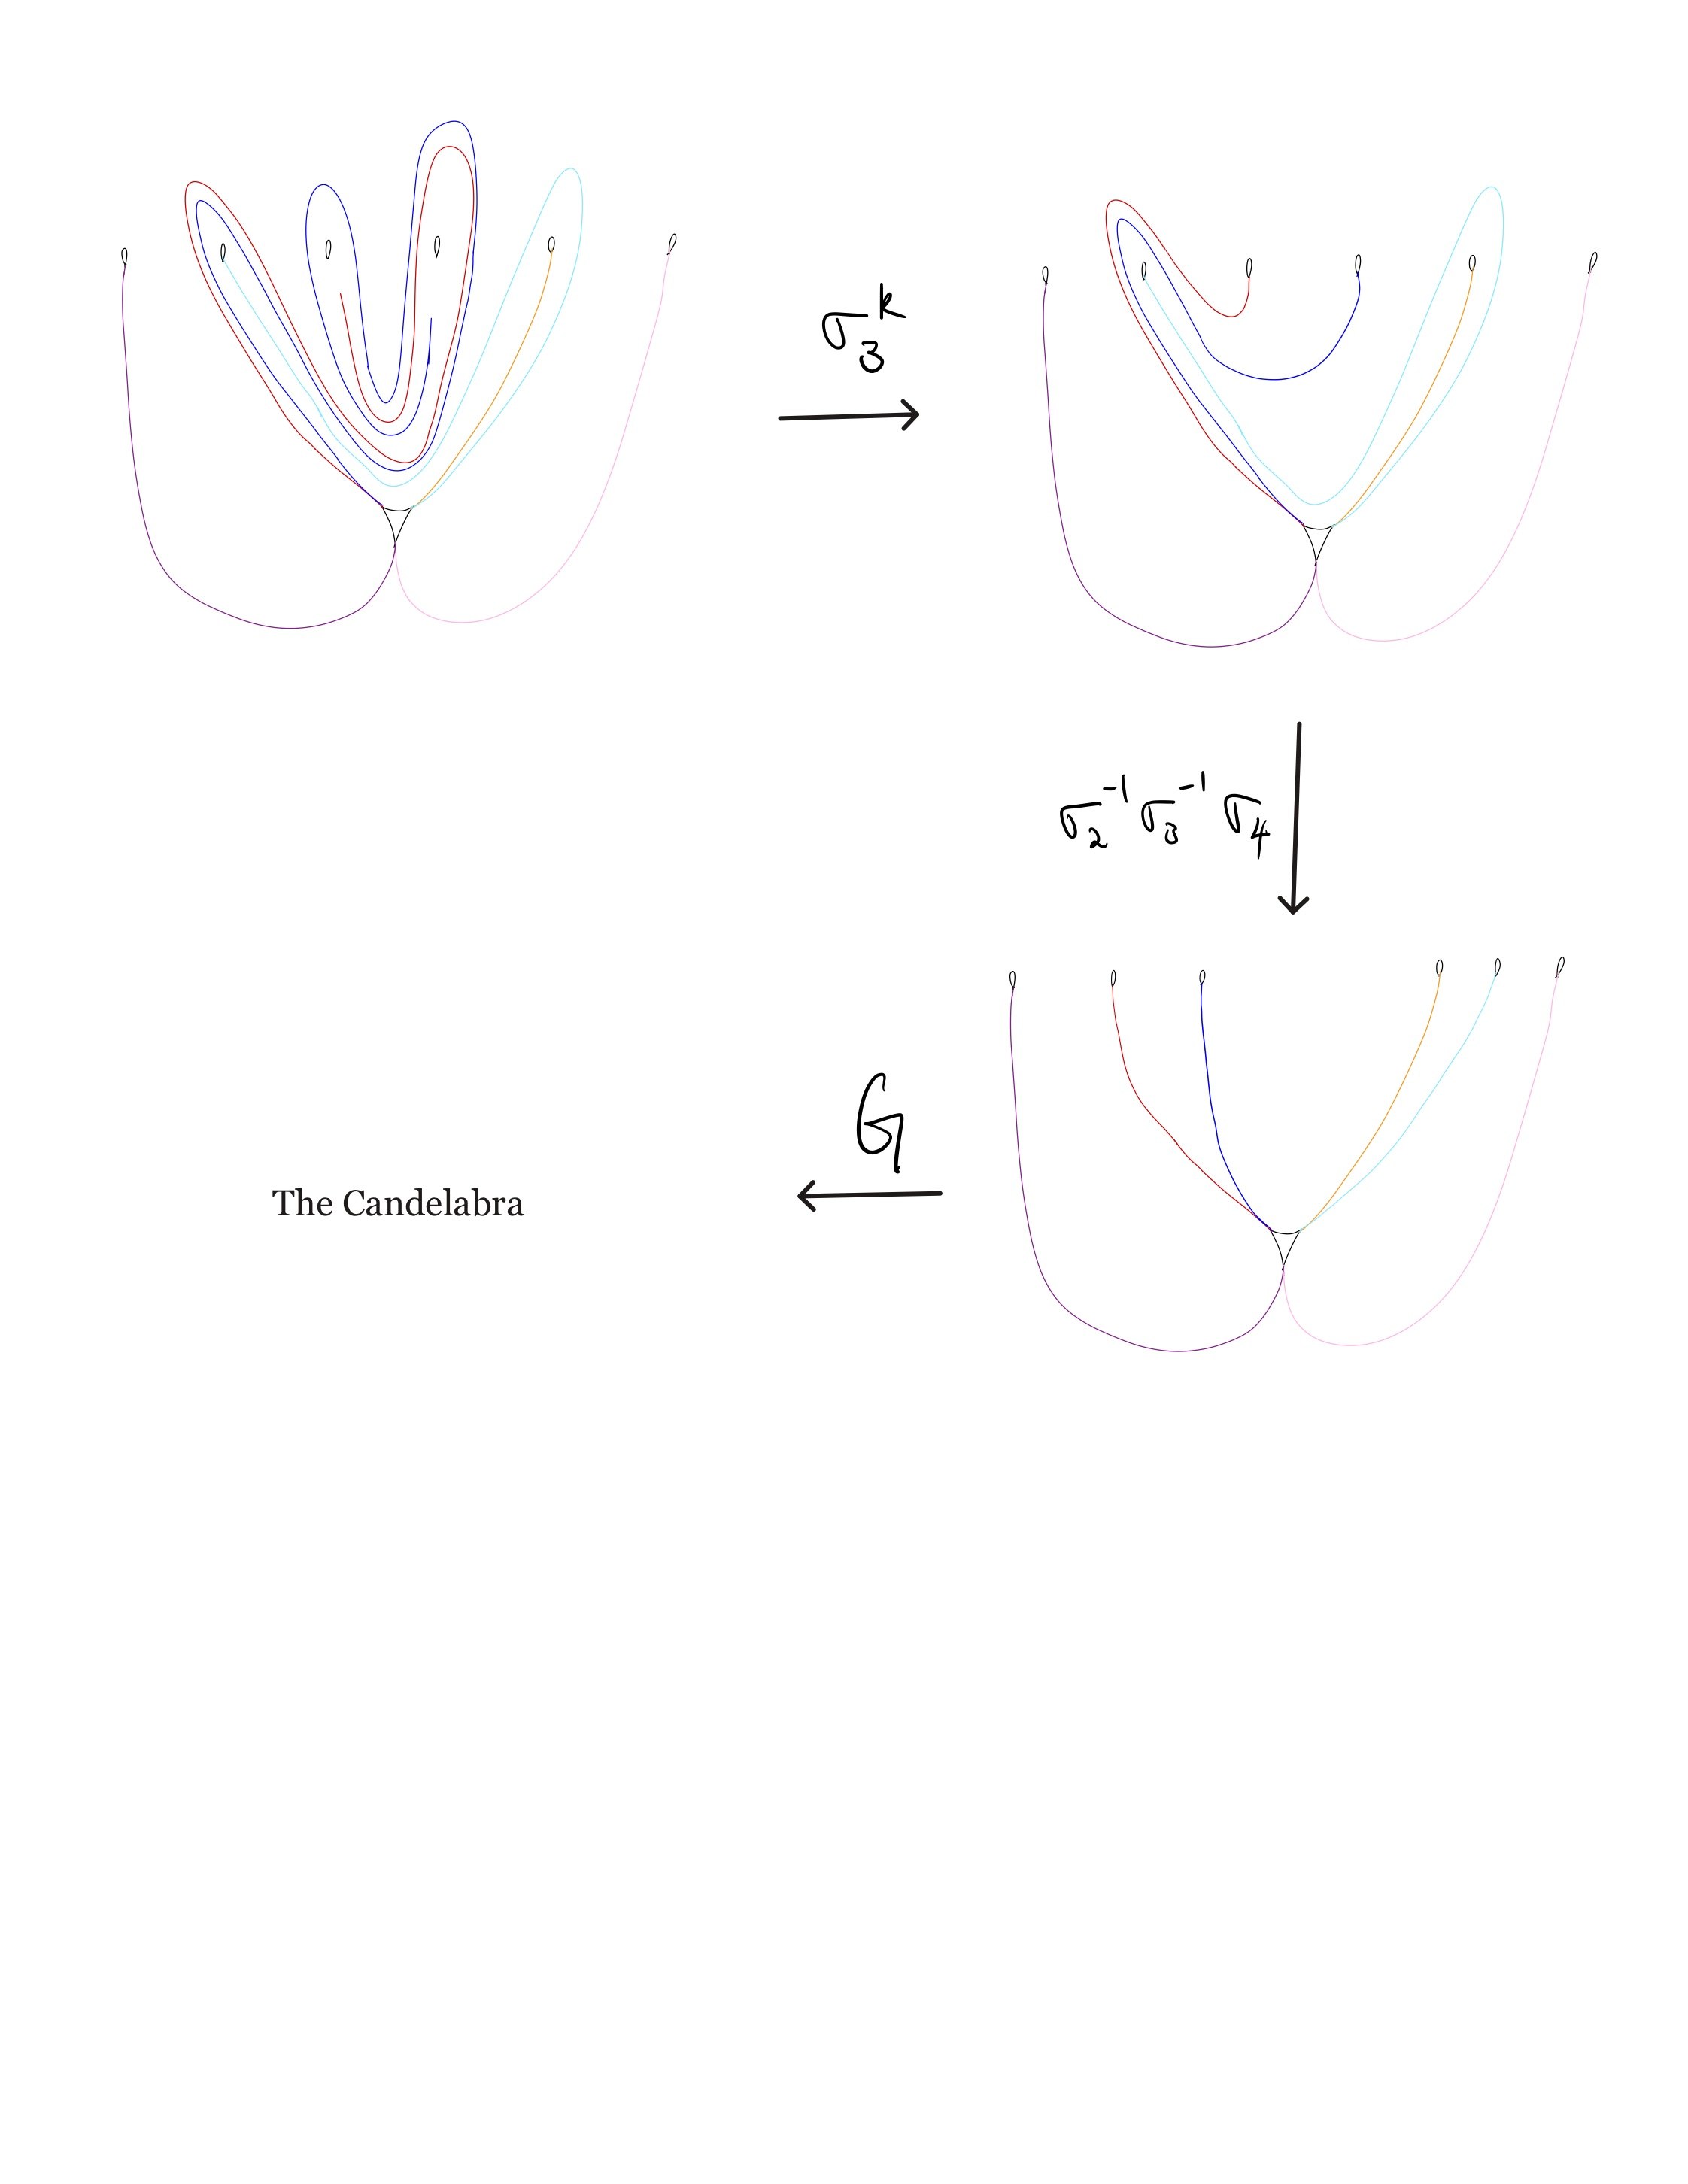
\includegraphics[width=\linewidth, height=0.45\textheight, keepaspectratio]{figures_braid/figures_candelabra/Candelabra Braid 2 Jehu-2.jpg}
    \caption{This sequence shows the inverse of the braid $b_2^c$ carries Train Track Candidate Family 2.}
    \label{fig:candelabra_braid_b2}
\end{figure*}

\clearpage

\section{Candidate Family 3}
Train Track Map Candidate Family 3 of the Candelabra train track is shown in Figure \ref{fig:candelabra_braid_b3_map}. Note there is twisting between $\fbs$ and $\fbo$. See \ref{Dindle} for details.

\begin{figure*}[ht]
    \centering
    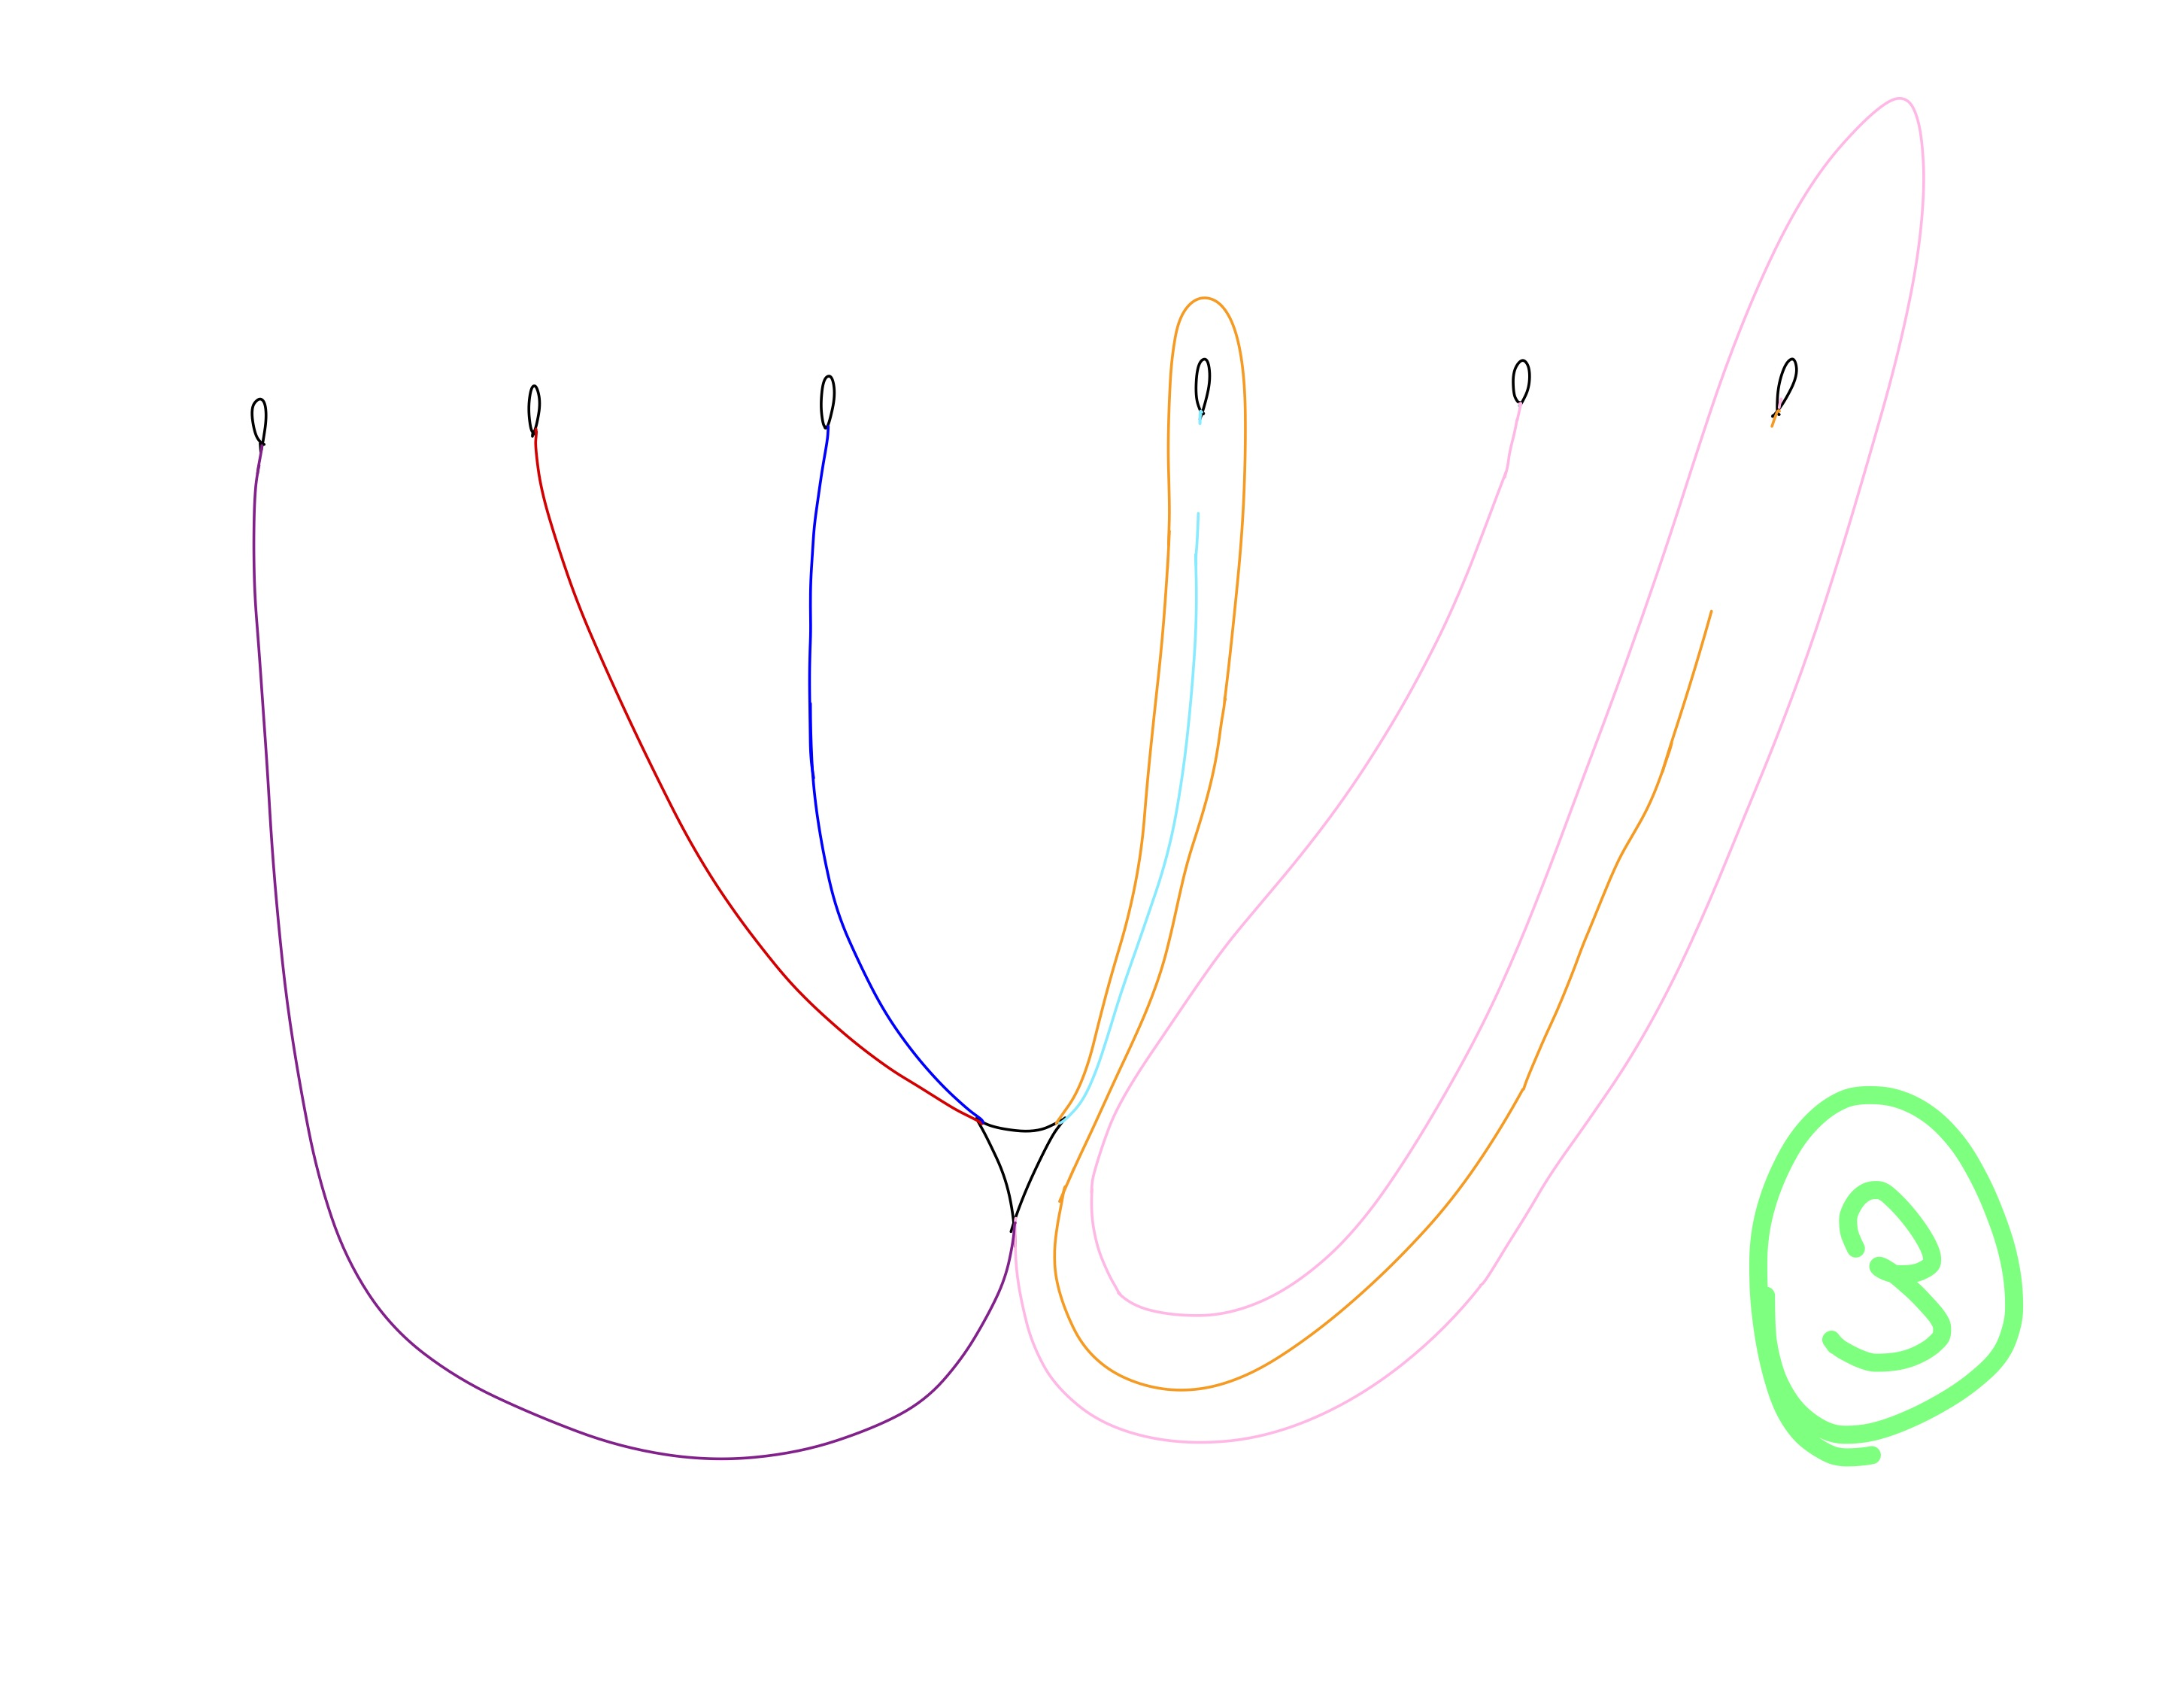
\includegraphics[width=\linewidth, height=0.45\textheight, keepaspectratio]{figures_braid/figures_candelabra/Candelabra Braid 3 Dindle-1.jpg}
    \caption{Train Track Map Candidate Family 3 of the Candelabra.}
    \label{fig:candelabra_braid_b3_map}
\end{figure*}

The inverse of the following braid carries this family of train track maps:
\[
b_3^c = \sigma_5 (\sigma_4^{-1})^k \circ G
\]
where $G$ is the braid of Section \ref{sec:braid G}, and $k\geq 1$ ($k\in \mathbb{Z}$) is the twisting parameter. This is shown in Figure \ref{fig:candelabra_braid_b3}

\begin{figure*}[p]
    \centering
    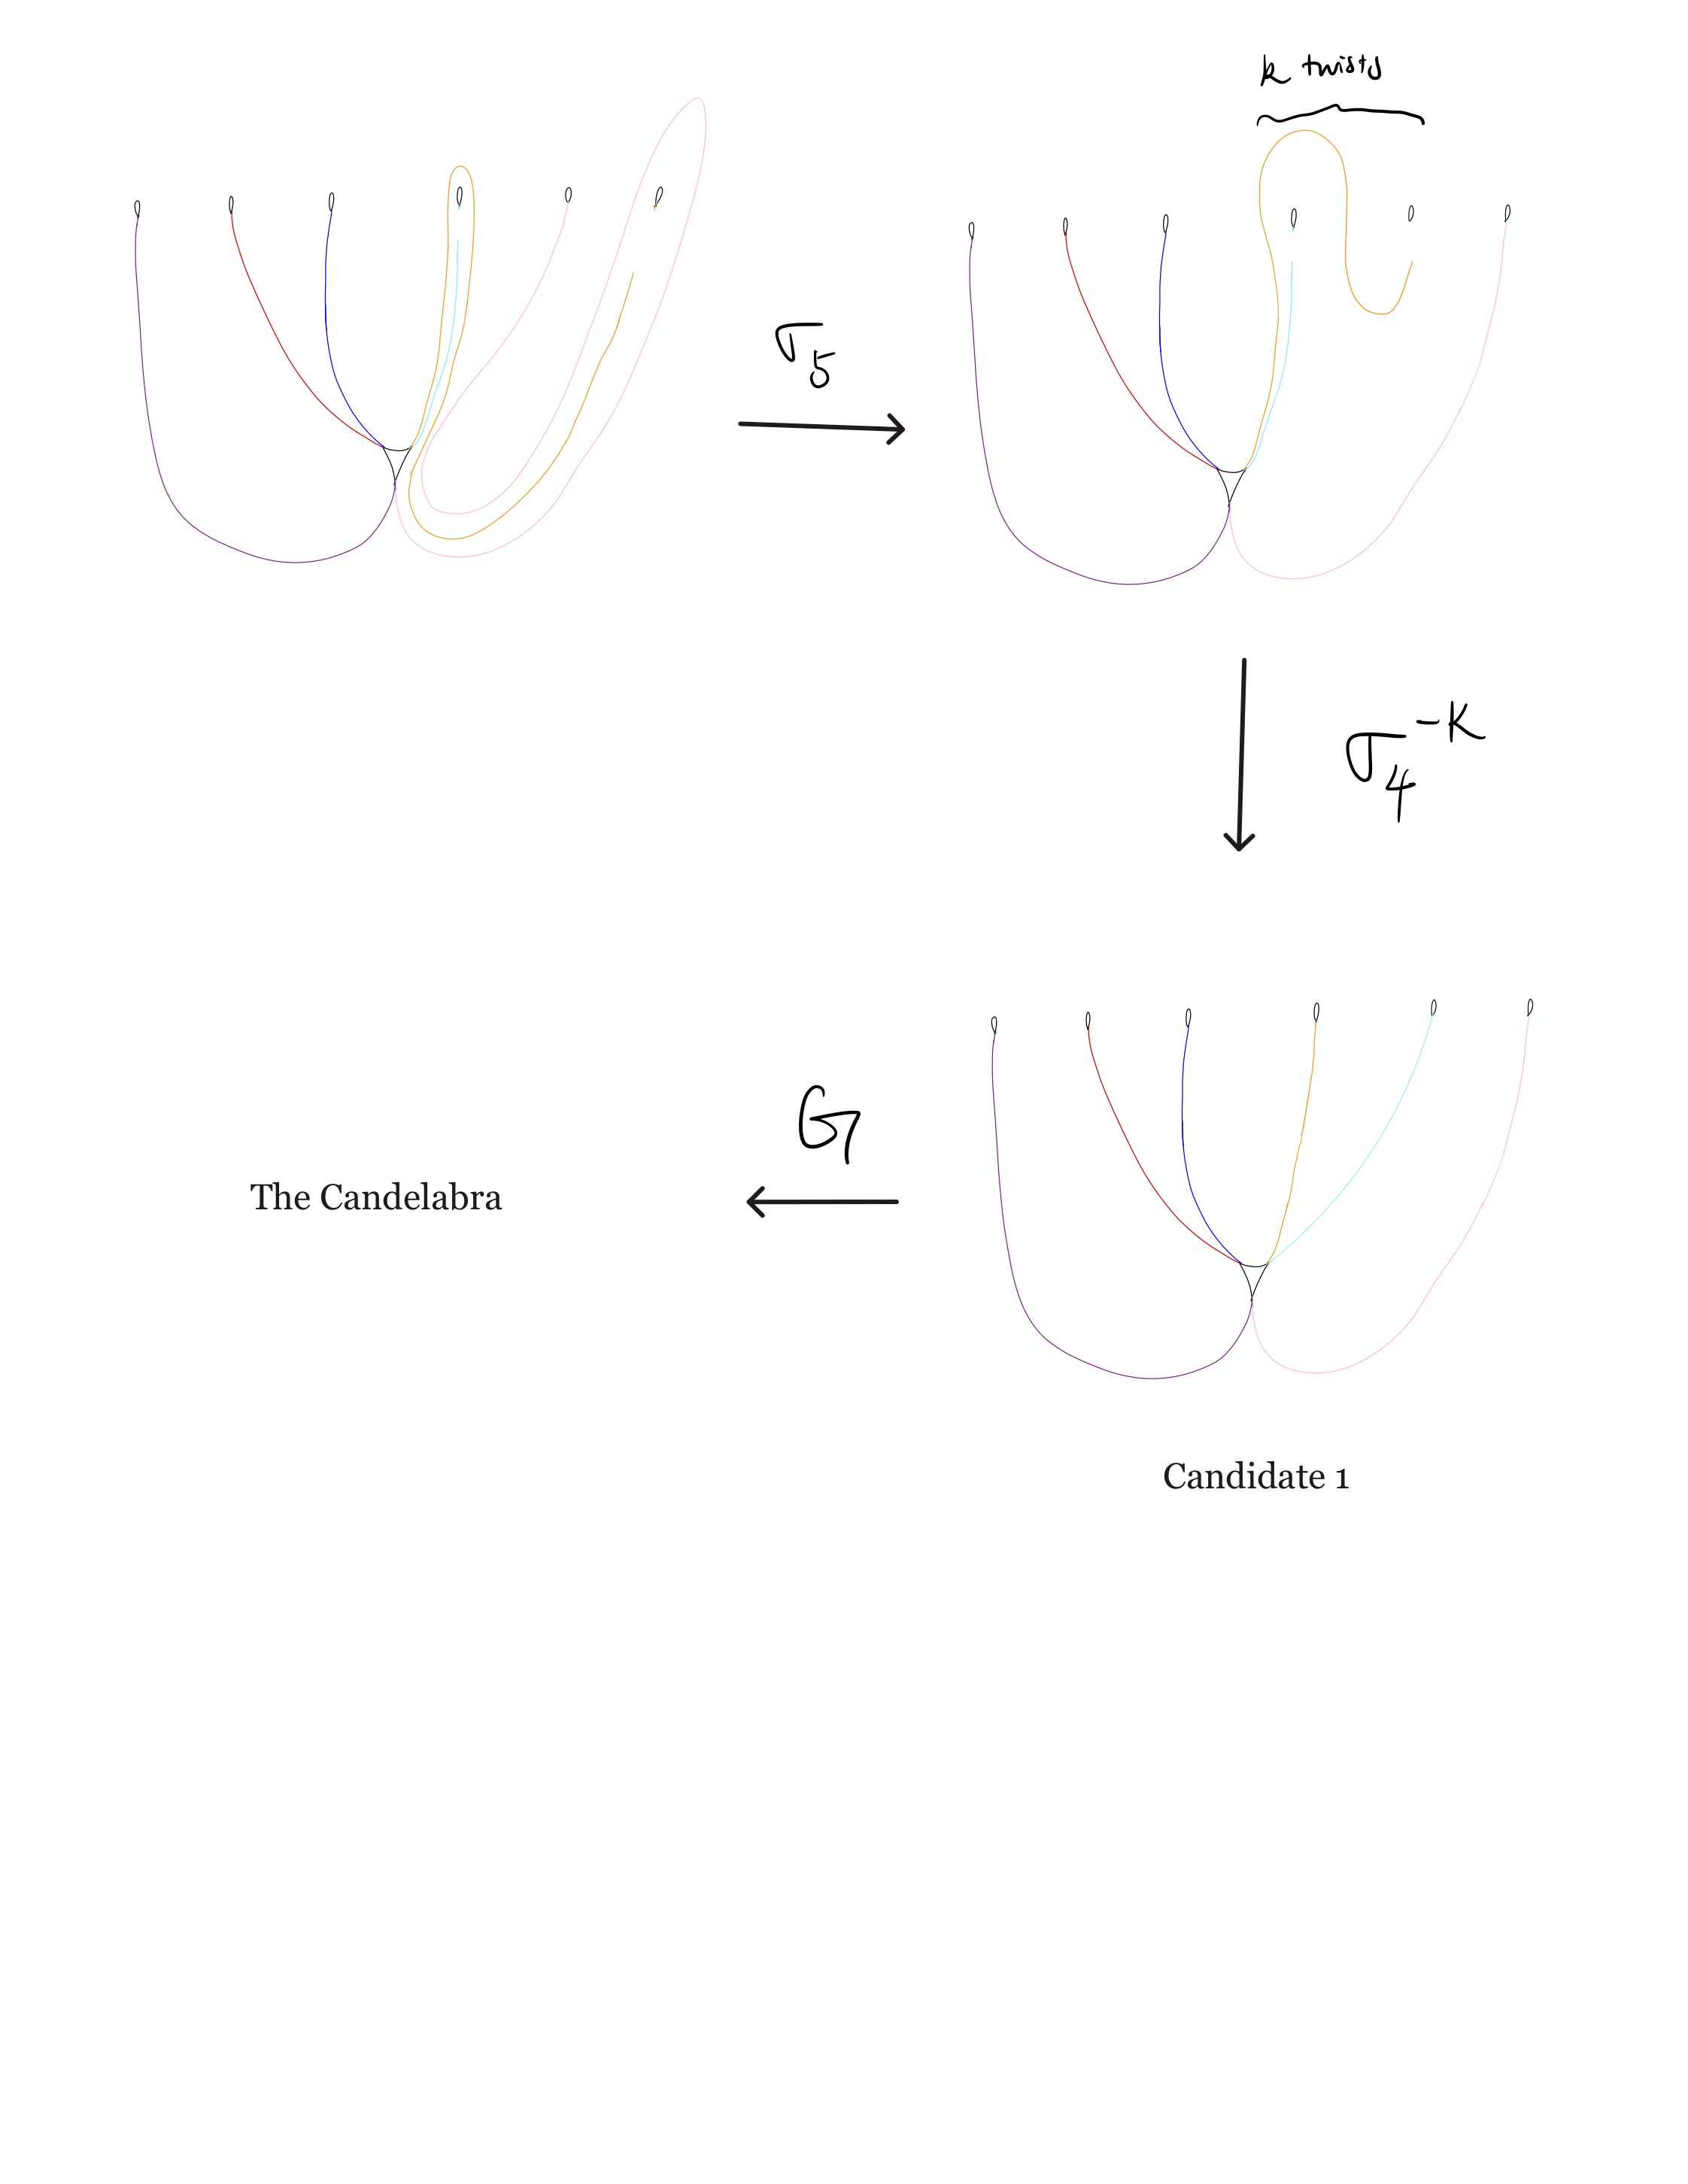
\includegraphics[width=\linewidth, height=0.45\textheight, keepaspectratio]{figures_braid/figures_candelabra/Candelabra Braid 3 Dindle-2.jpg}
    \caption{This sequence shows the inverse of the braid $b_3^c$ carries Train Track Candidate Family 3.}
    \label{fig:candelabra_braid_b3}
\end{figure*}

\clearpage

\section{Candidate Family 4}
Train Track Map Candidate Family 4 of the Candelabra train track is shown in Figure \ref{fig:candelabra_braid_b4_map}. Note there is twisting between $\fbo$ and $\fbi$. See \ref{Keffel} for details.

\begin{figure*}[ht]
    \centering
    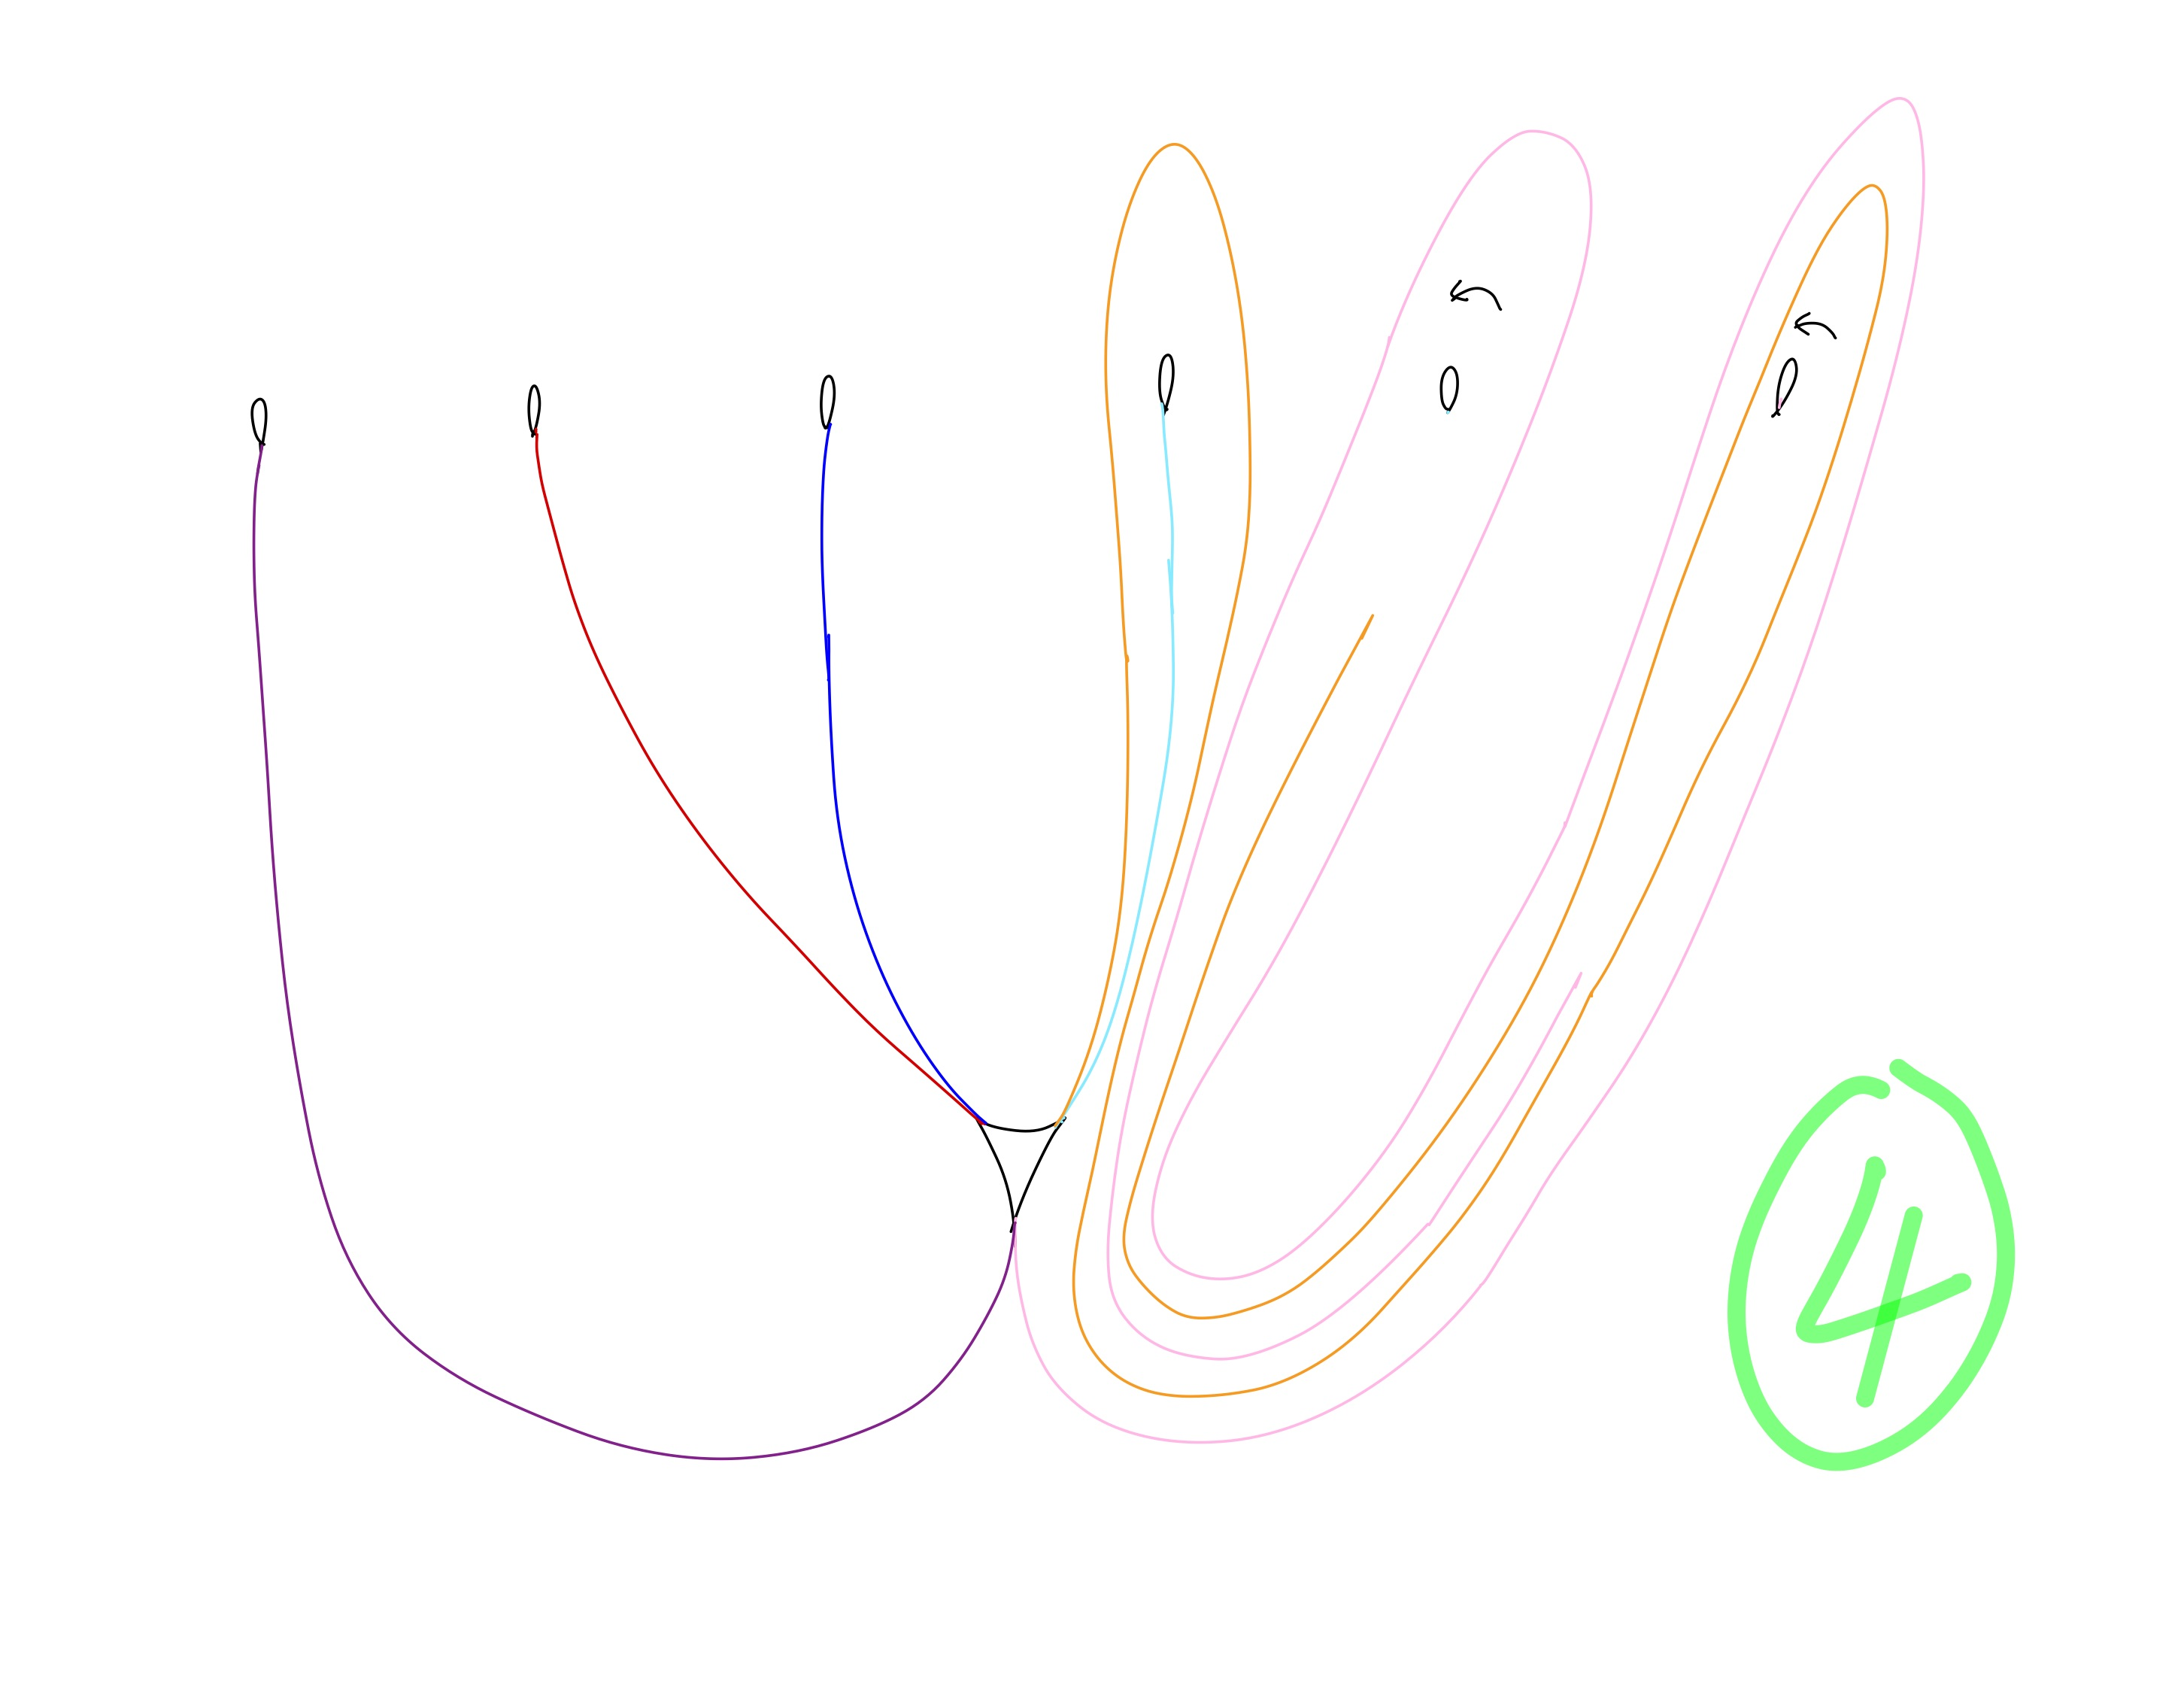
\includegraphics[width=\linewidth, height=0.45\textheight, keepaspectratio]{figures_braid/figures_candelabra/Candelabra Braid 4 Keffel-1.jpg}
    \caption{Train Track Map Candidate Family 4 of the Candelabra.}
    \label{fig:candelabra_braid_b4_map}
\end{figure*}

The inverse of the following braid carries this family of train track maps:
\[
b_4^c = (\sigma_5^{-1})^k \sigma_4 \circ G
\]
where $G$ is the braid of Section \ref{sec:braid G}, and $k\geq 1$ ($k\in \mathbb{Z}$) is the twisting parameter. This is shown in Figure \ref{fig:candelabra_braid_b4}

\begin{figure*}[p]
    \centering
    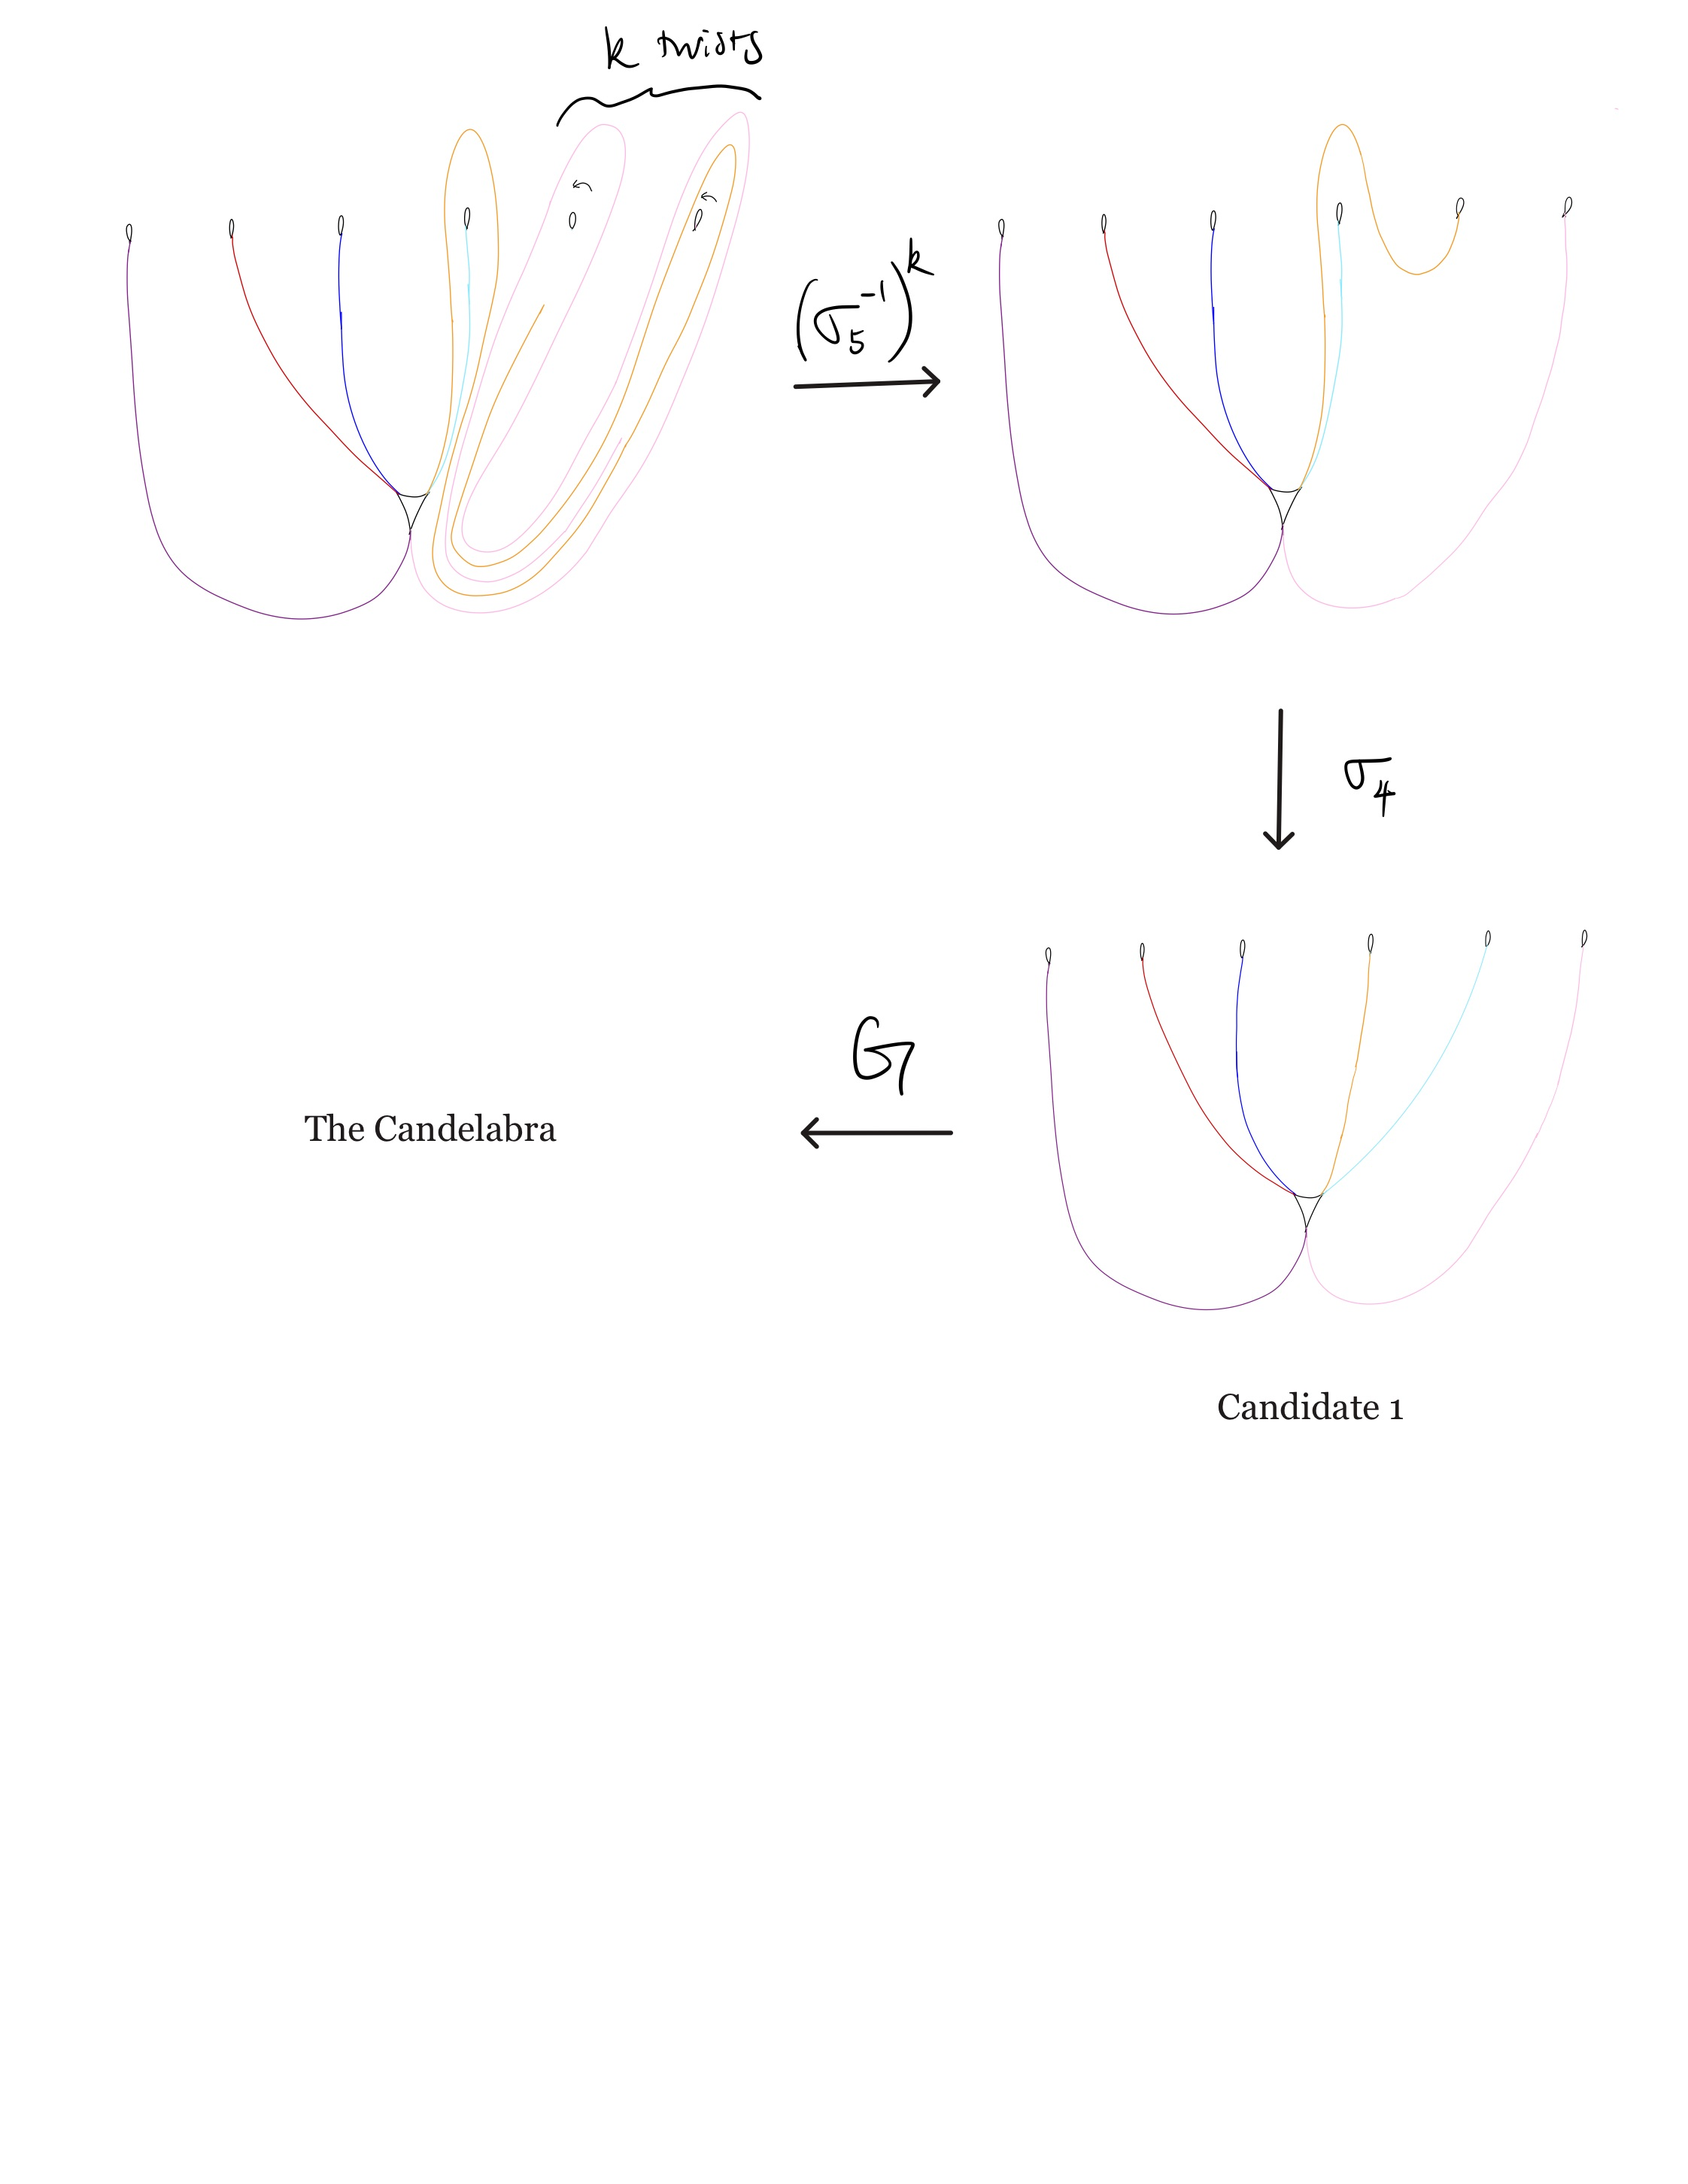
\includegraphics[width=\linewidth, height=0.45\textheight, keepaspectratio]{figures_braid/figures_candelabra/Candelabra Braid 4 Keffel-2.jpg}  
    \caption{This sequence shows the inverse of the braid $b_4^c$ carries Train Track Candidate Family 4.}
    \label{fig:candelabra_braid_b4}
\end{figure*}

\clearpage

\section{Candidate Family 5}
Train Track Map Candidate Family 5 of the Candelabra train track is shown in Figure \ref{fig:candelabra_braid_b5_map}. Note there is twisting among $\fbs$,$\fbi$, and $\fbo$. See \ref{Keffel} for details.

\begin{figure*}[ht]
    \centering
    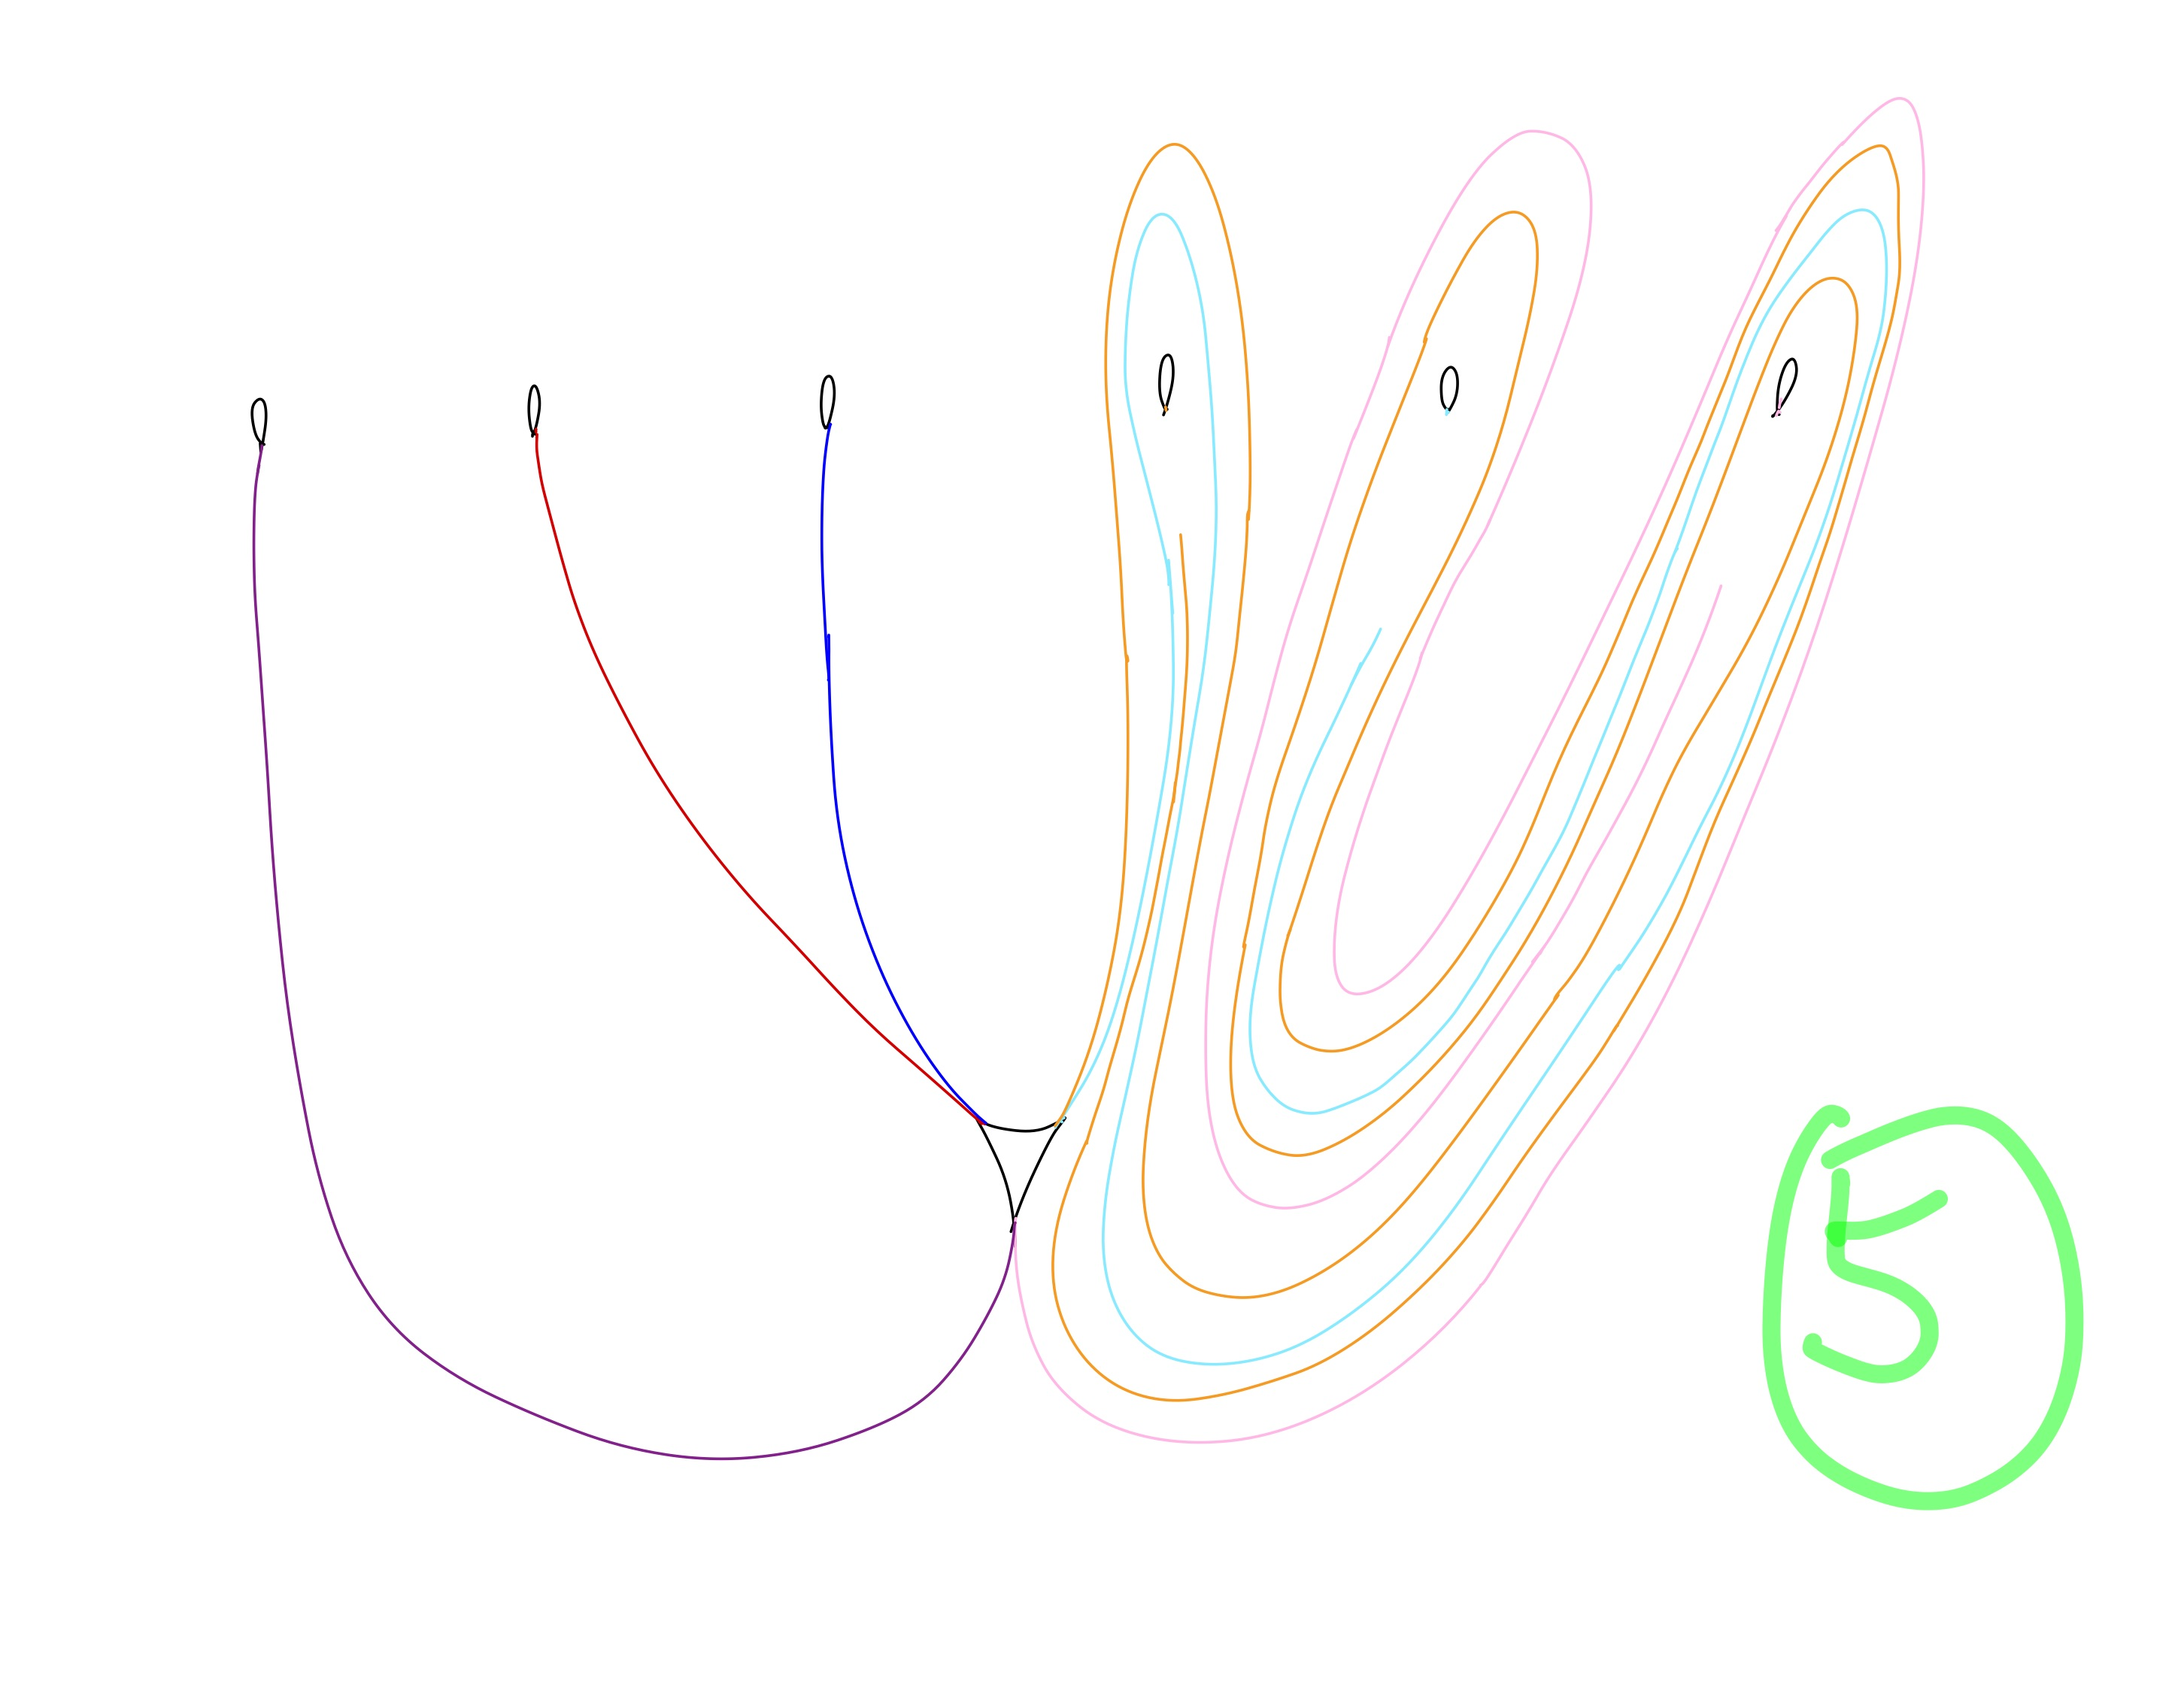
\includegraphics[width=\linewidth, height=0.45\textheight, keepaspectratio]{figures_braid/figures_candelabra/Candelabra Braid 5 Keffel-1.jpg}
    \caption{Train Track Map Candidate Family 5 of the Candelabra.}
    \label{fig:candelabra_braid_b5_map}
\end{figure*}

The inverse of the following braid carries this family of train track maps:
\[
b_5^c = (\sigma_5^{-1})^k\sigma_4^m\sigma_4^{-1} \circ G
\]
where $G$ is the braid of Section \ref{sec:braid G}, and $k,m \geq 1$ ($k,m \in \mathbb{Z}$) are the twisting parameters. This is shown in Figure \ref{fig:candelabra_braid_b5}

\begin{figure*}[p]
    \centering
    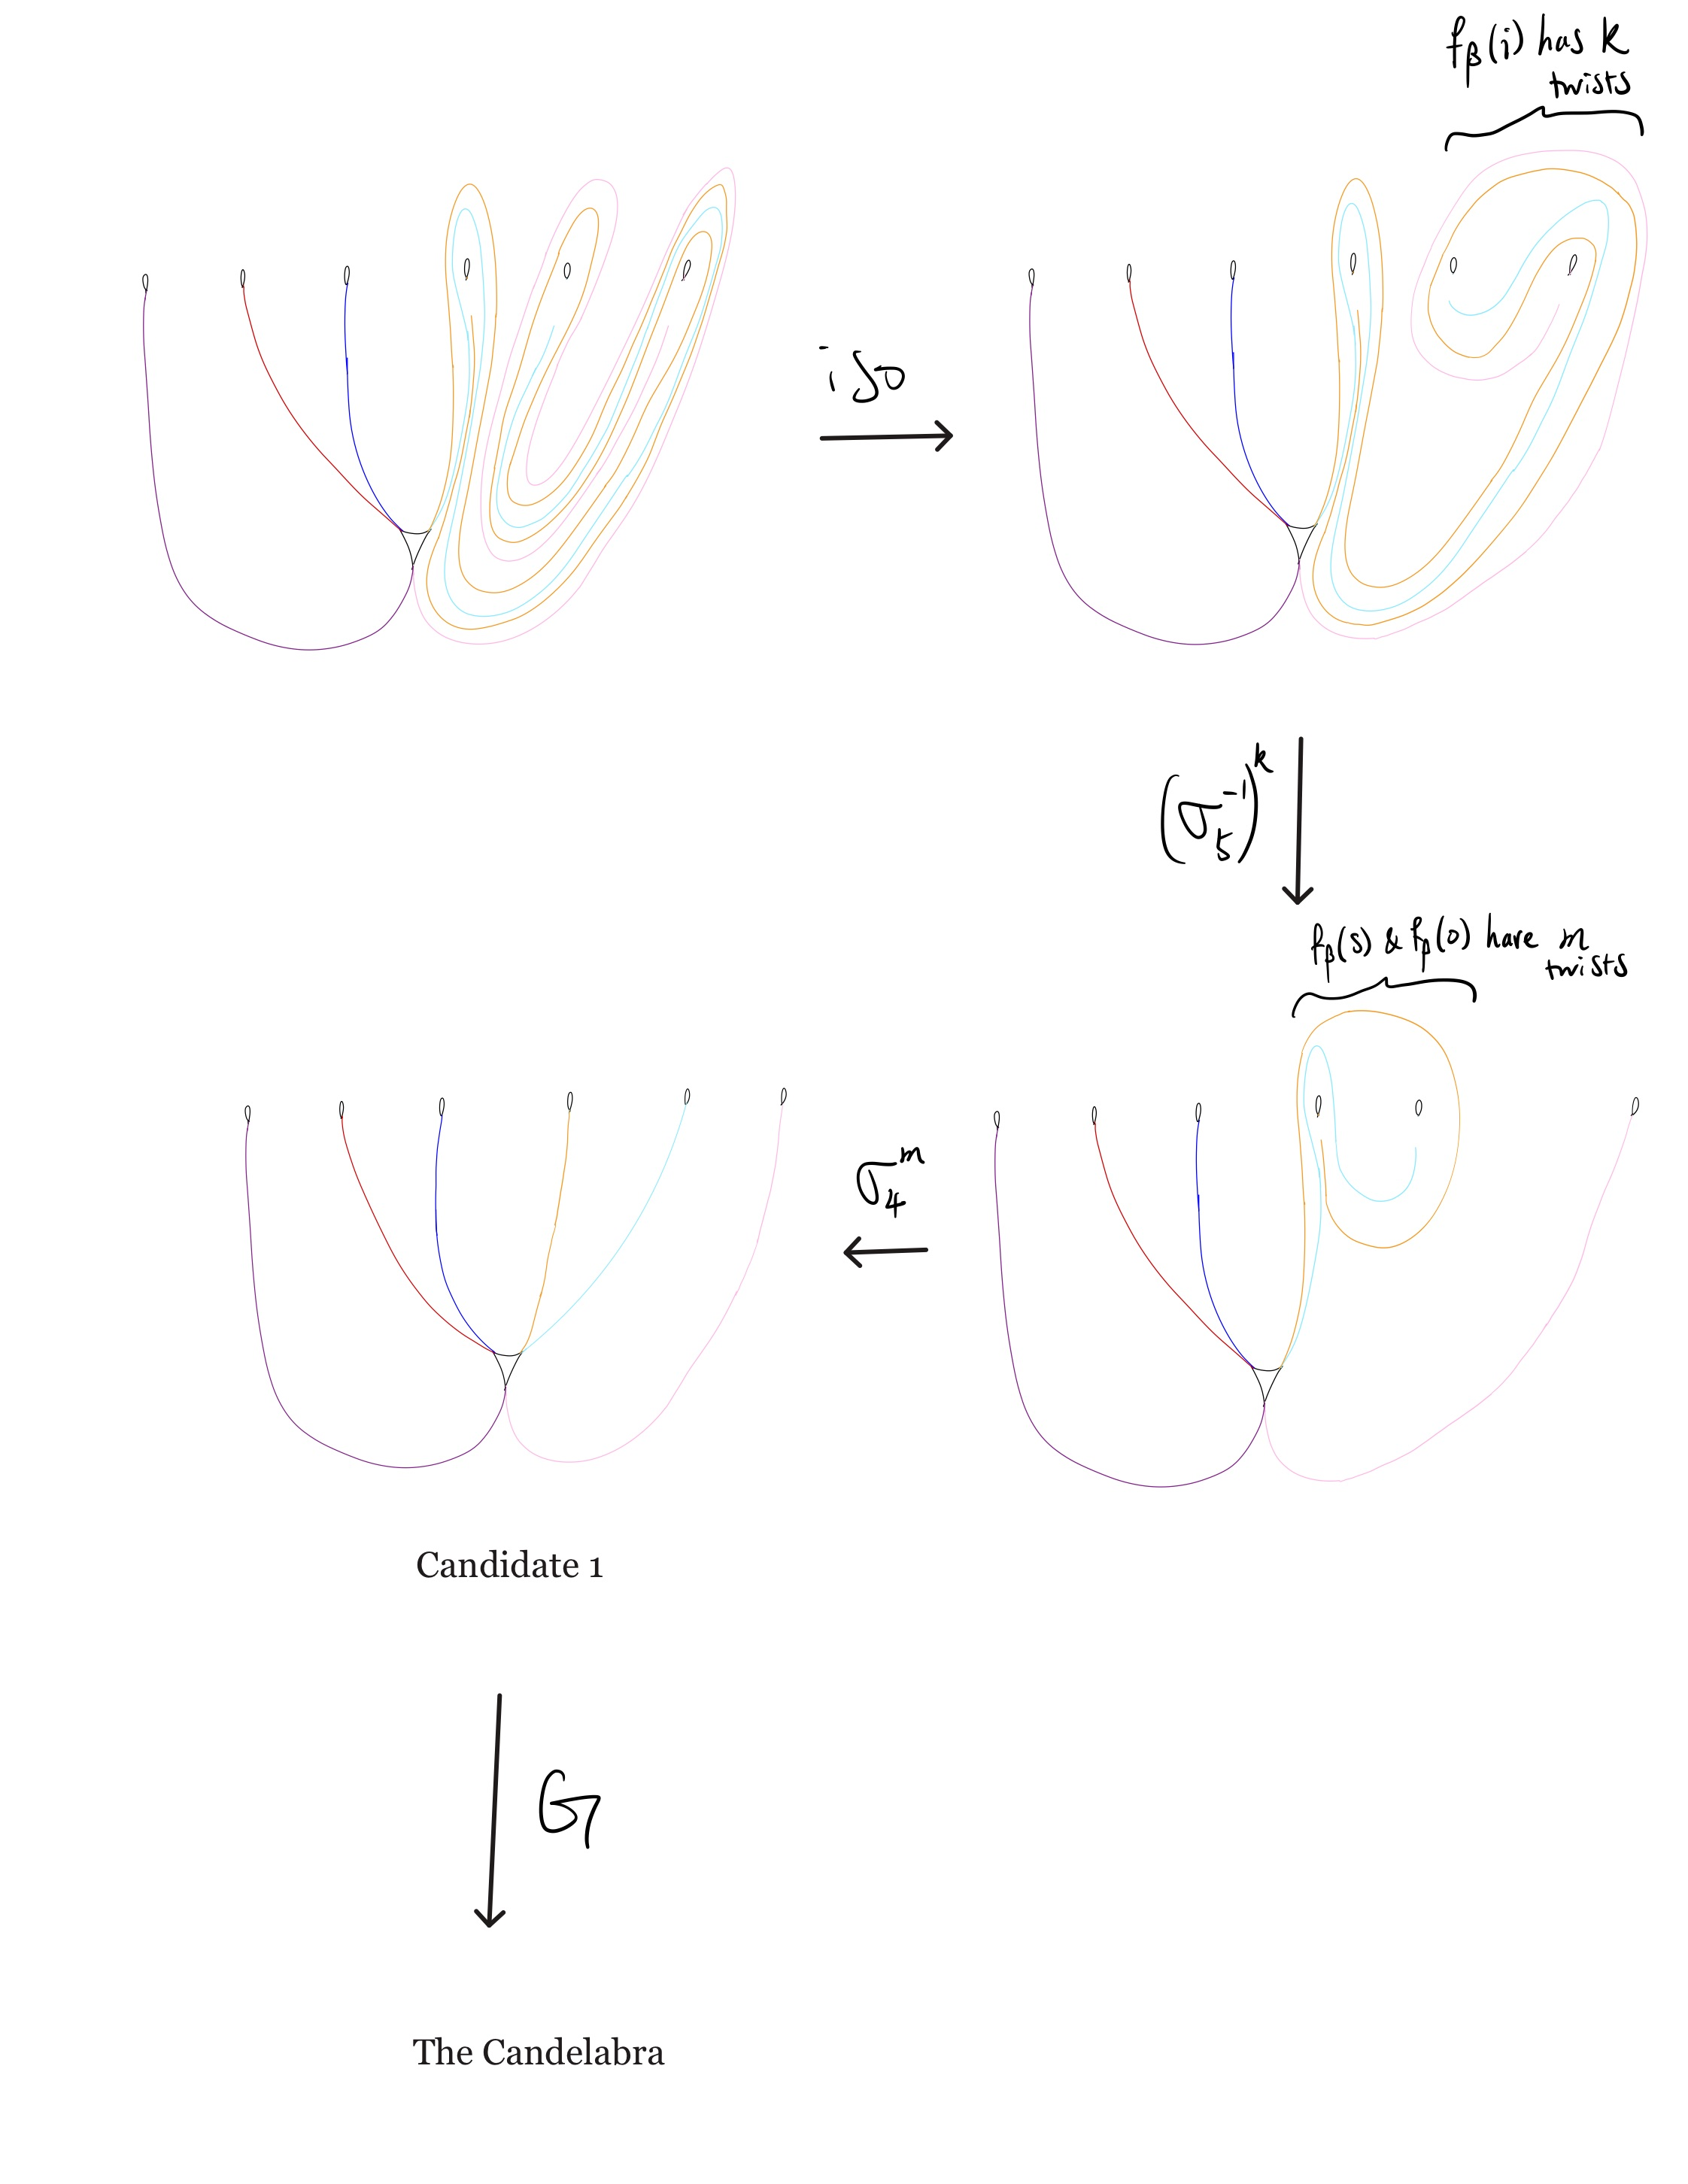
\includegraphics[width=\linewidth, height=0.45\textheight, keepaspectratio]{figures_braid/figures_candelabra/Candelabra Braid 5 Keffel-2.jpg}
    \caption{This sequence shows the inverse of the braid $b_5^c$ carries Train Track Candidate Family 5.}
    \label{fig:candelabra_braid_b5}
\end{figure*}

\clearpage

\section{Candidate Family 6}
Train Track Map Candidate Family 6 of the Candelabra train track is shown in Figure \ref{fig:candelabra_braid_b6_map}. Note there is twisting between $\fbb$ and $\fbr$. See \ref{Epigone} for details.

\begin{figure*}[ht]
    \centering
    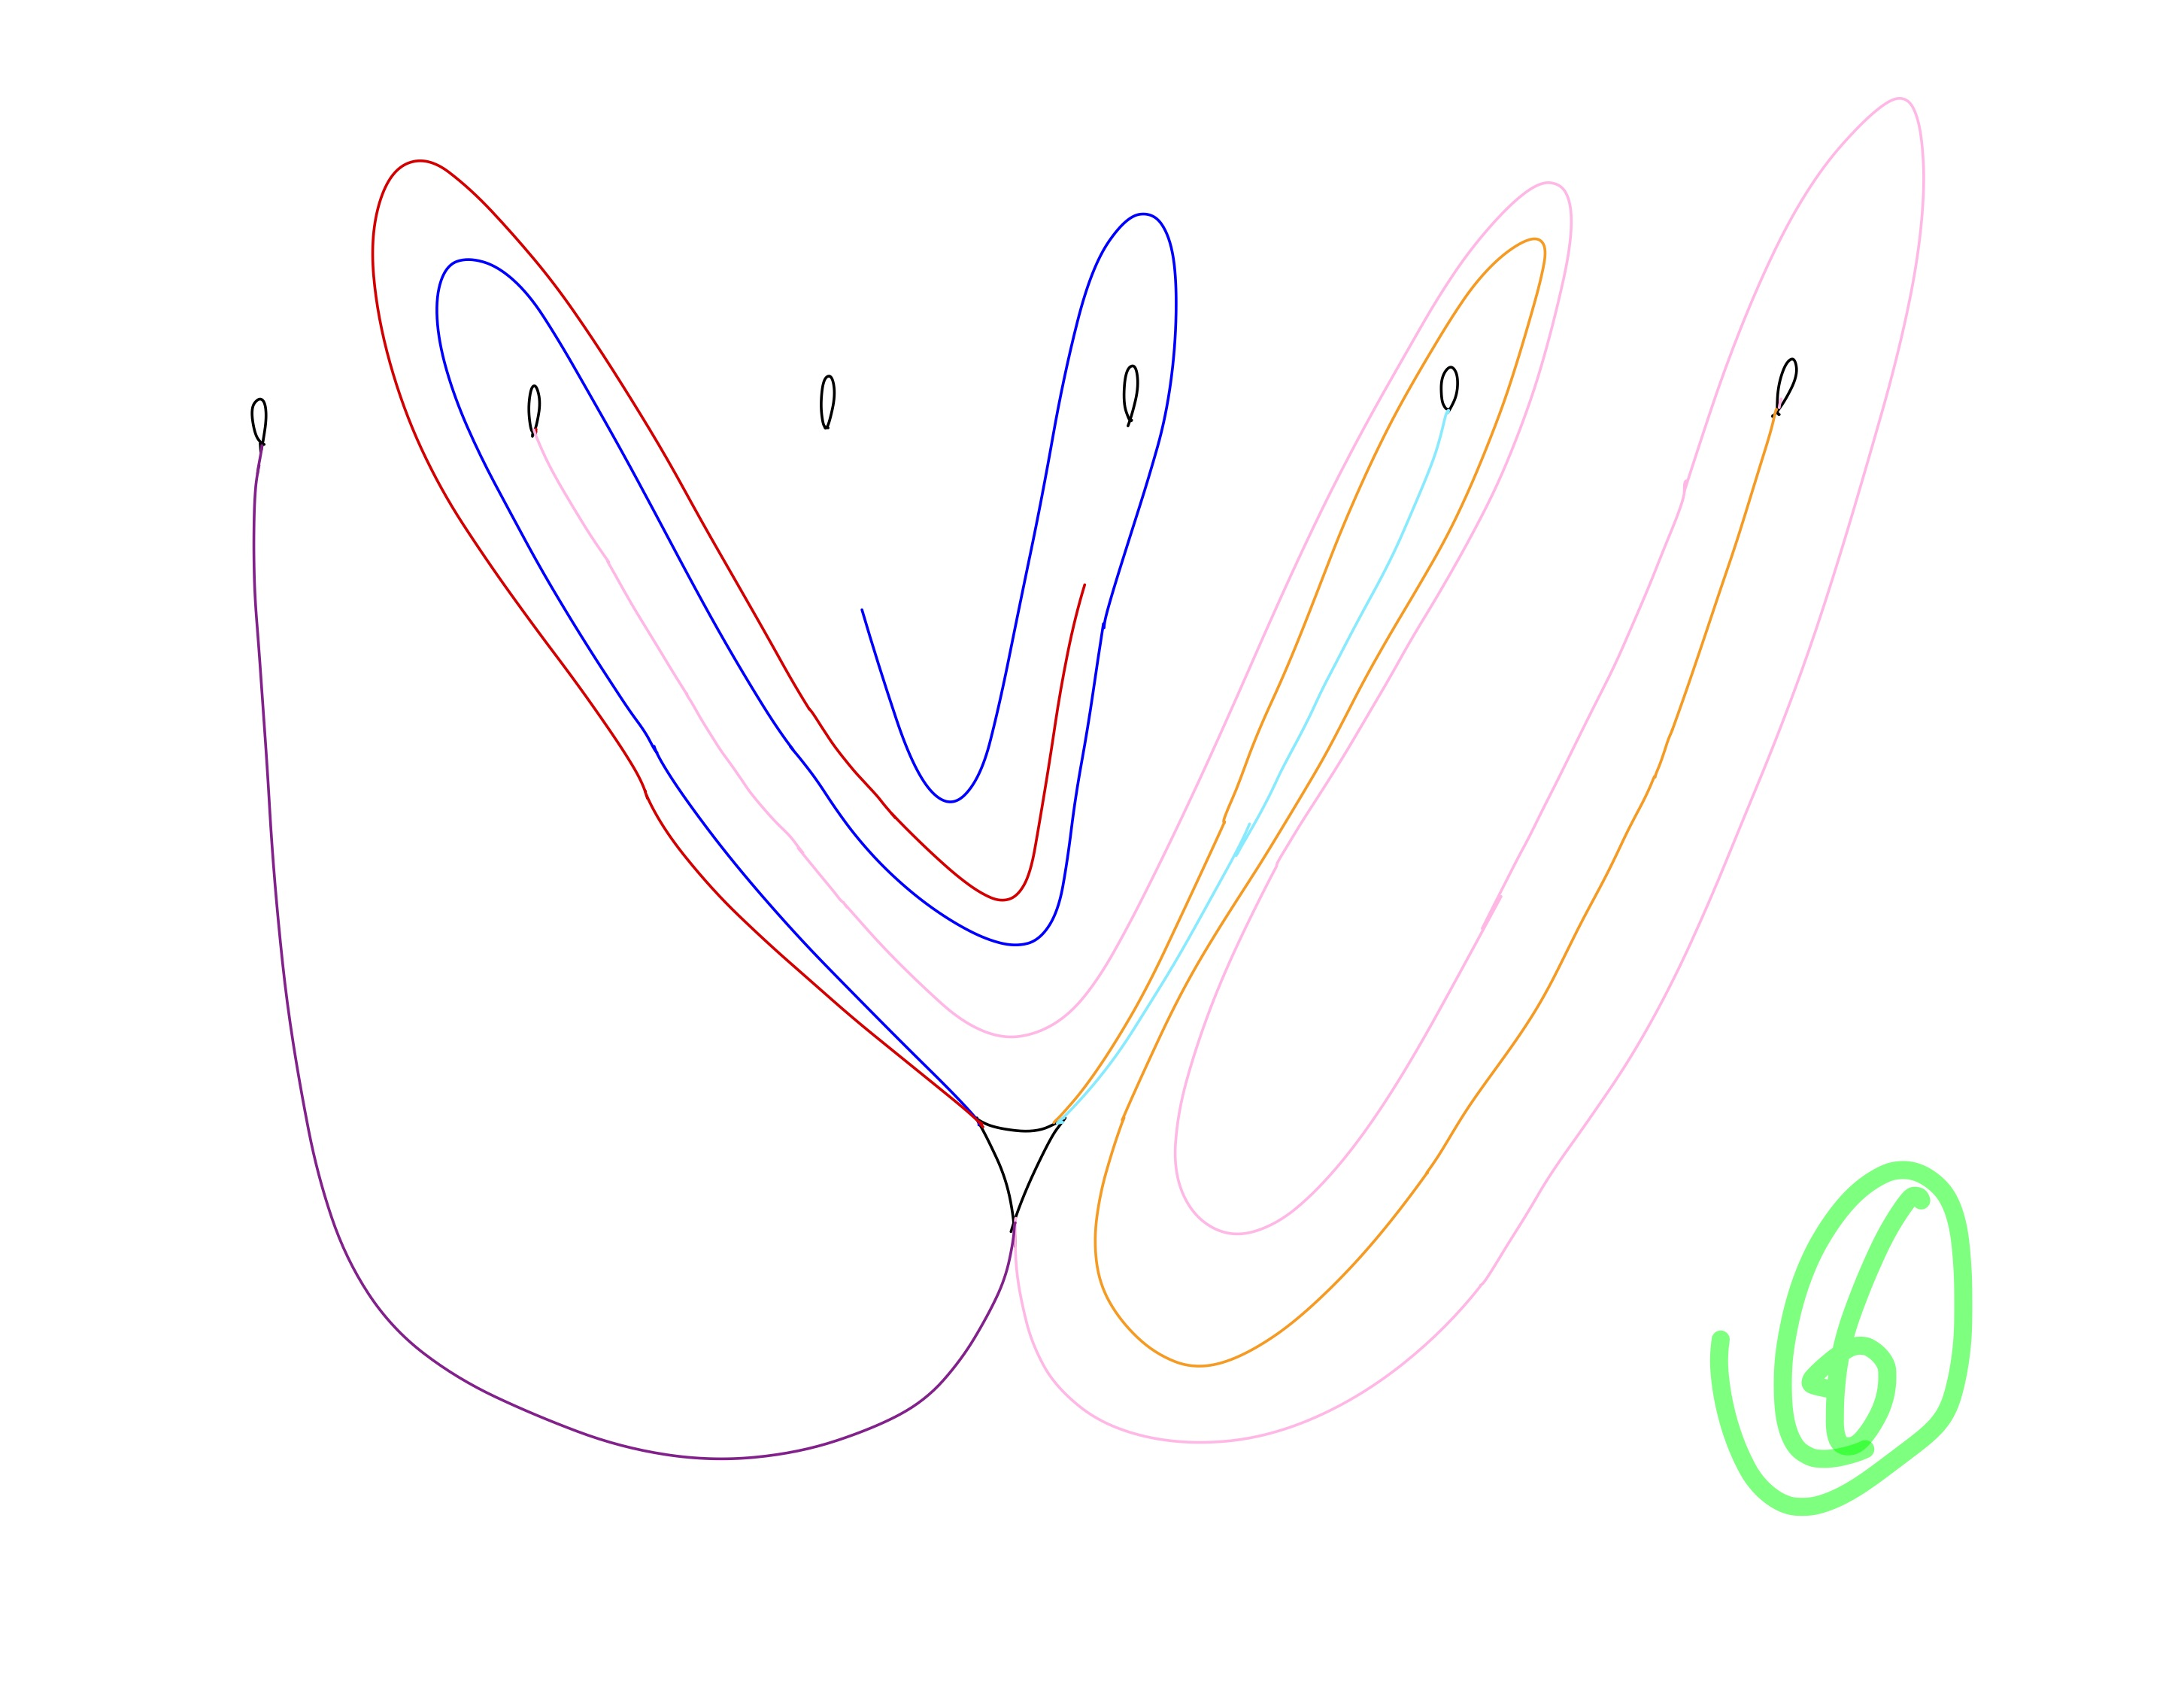
\includegraphics[width=\linewidth, height=0.45\textheight, keepaspectratio]{figures_braid/figures_candelabra/Candelabra Braid 6 Epigone-1.jpg}
    \caption{Train Track Map Candidate Family 6 of the Candelabra.}
    \label{fig:candelabra_braid_b6_map}
\end{figure*}

The inverse of the following braid carries this family of train track maps:
\[
b_6^c = (\sigma_{3}^{-1})^k \sigma_{2} \sigma_{3} \sigma_{4}^{-1} \sigma_{5}^{-1} \sigma_{4} \circ G
\]
where $G$ is the braid of Section \ref{sec:braid G}, and $k\geq 1$ ($k\in \mathbb{Z}$) is the twisting parameter. This is shown in Figure \ref{fig:candelabra_braid_b6}

\begin{figure*}[p]
    \centering
    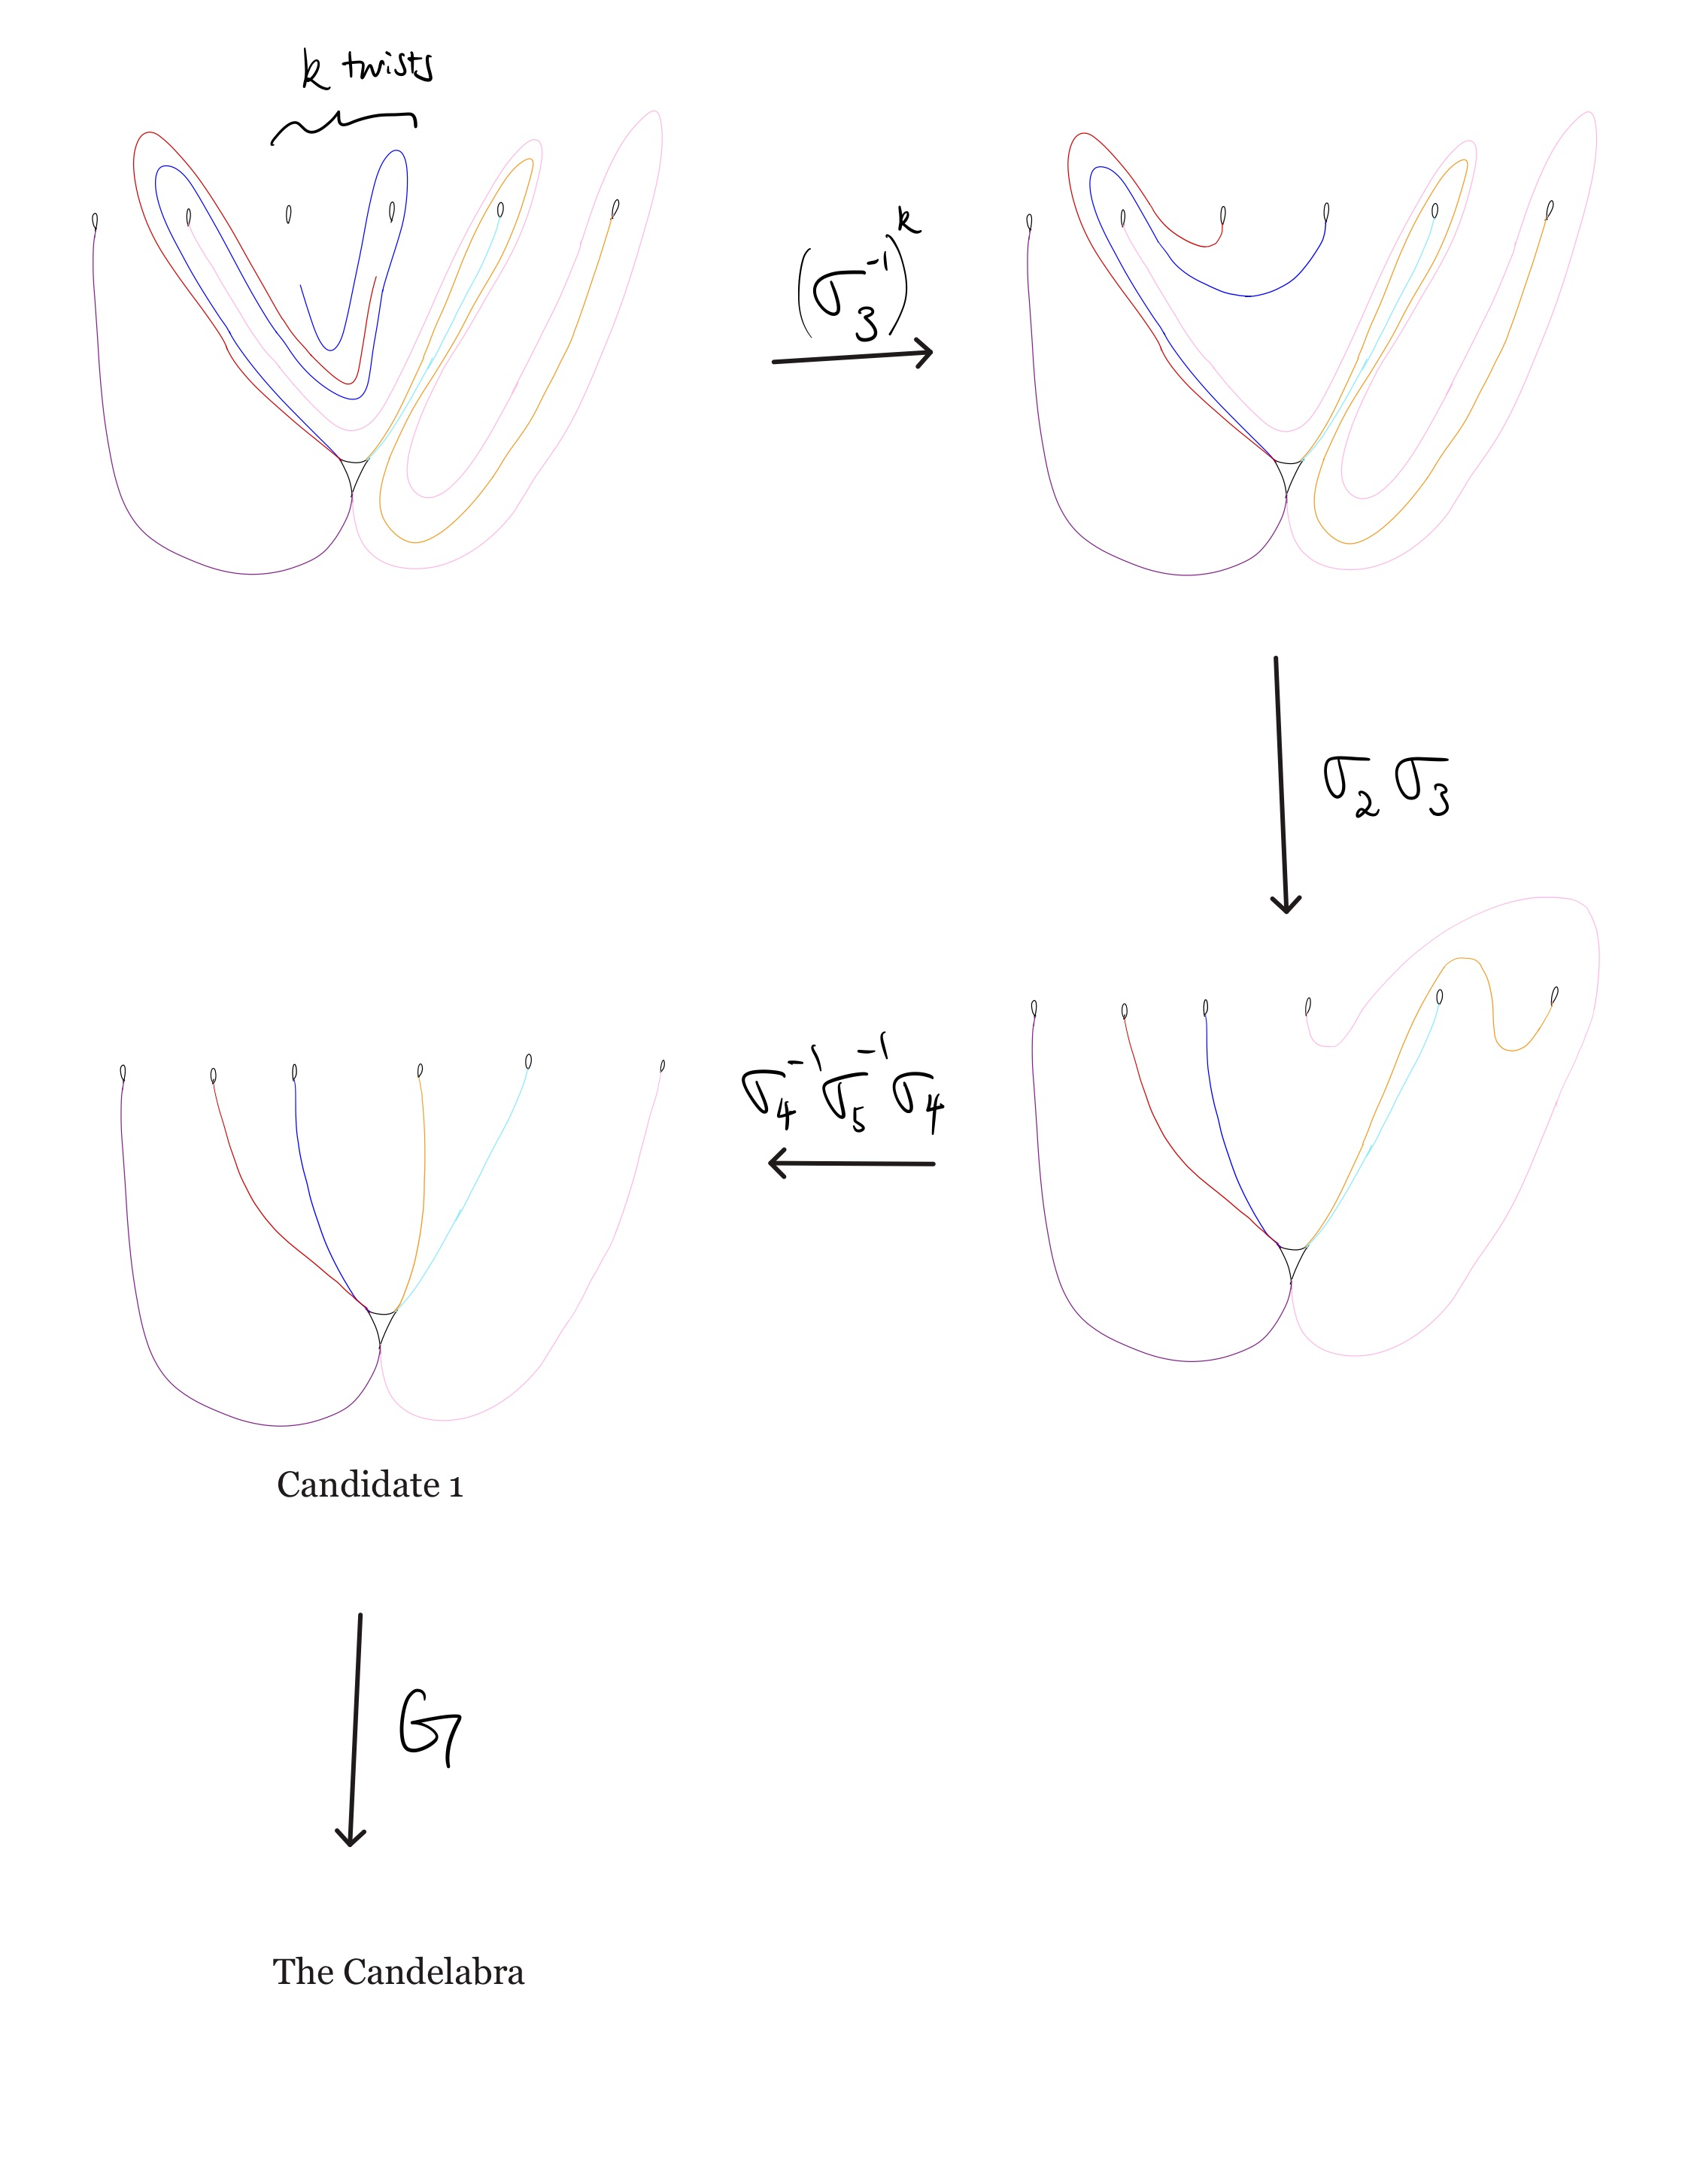
\includegraphics[width=\linewidth, height=0.45\textheight, keepaspectratio]{figures_braid/figures_candelabra/Candelabra Braid 6 Epigone-2.jpg}
    \caption{This sequence shows the inverse of the braid $b_6^c$ carries Train Track Candidate Family 6.}
    \label{fig:candelabra_braid_b6}
\end{figure*}

\clearpage

\section{Candidate Family 7}
Train Track Map Candidate Family 7 of the Candelabra train track is shown in Figure \ref{fig:candelabra_braid_b7_map}. Note there is twisting between $\fbb$ and $\fbr$, and twisting between $\fbo$ and $\fbs$. See \ref{Farrago} for details.

\begin{figure*}[ht]
    \centering
    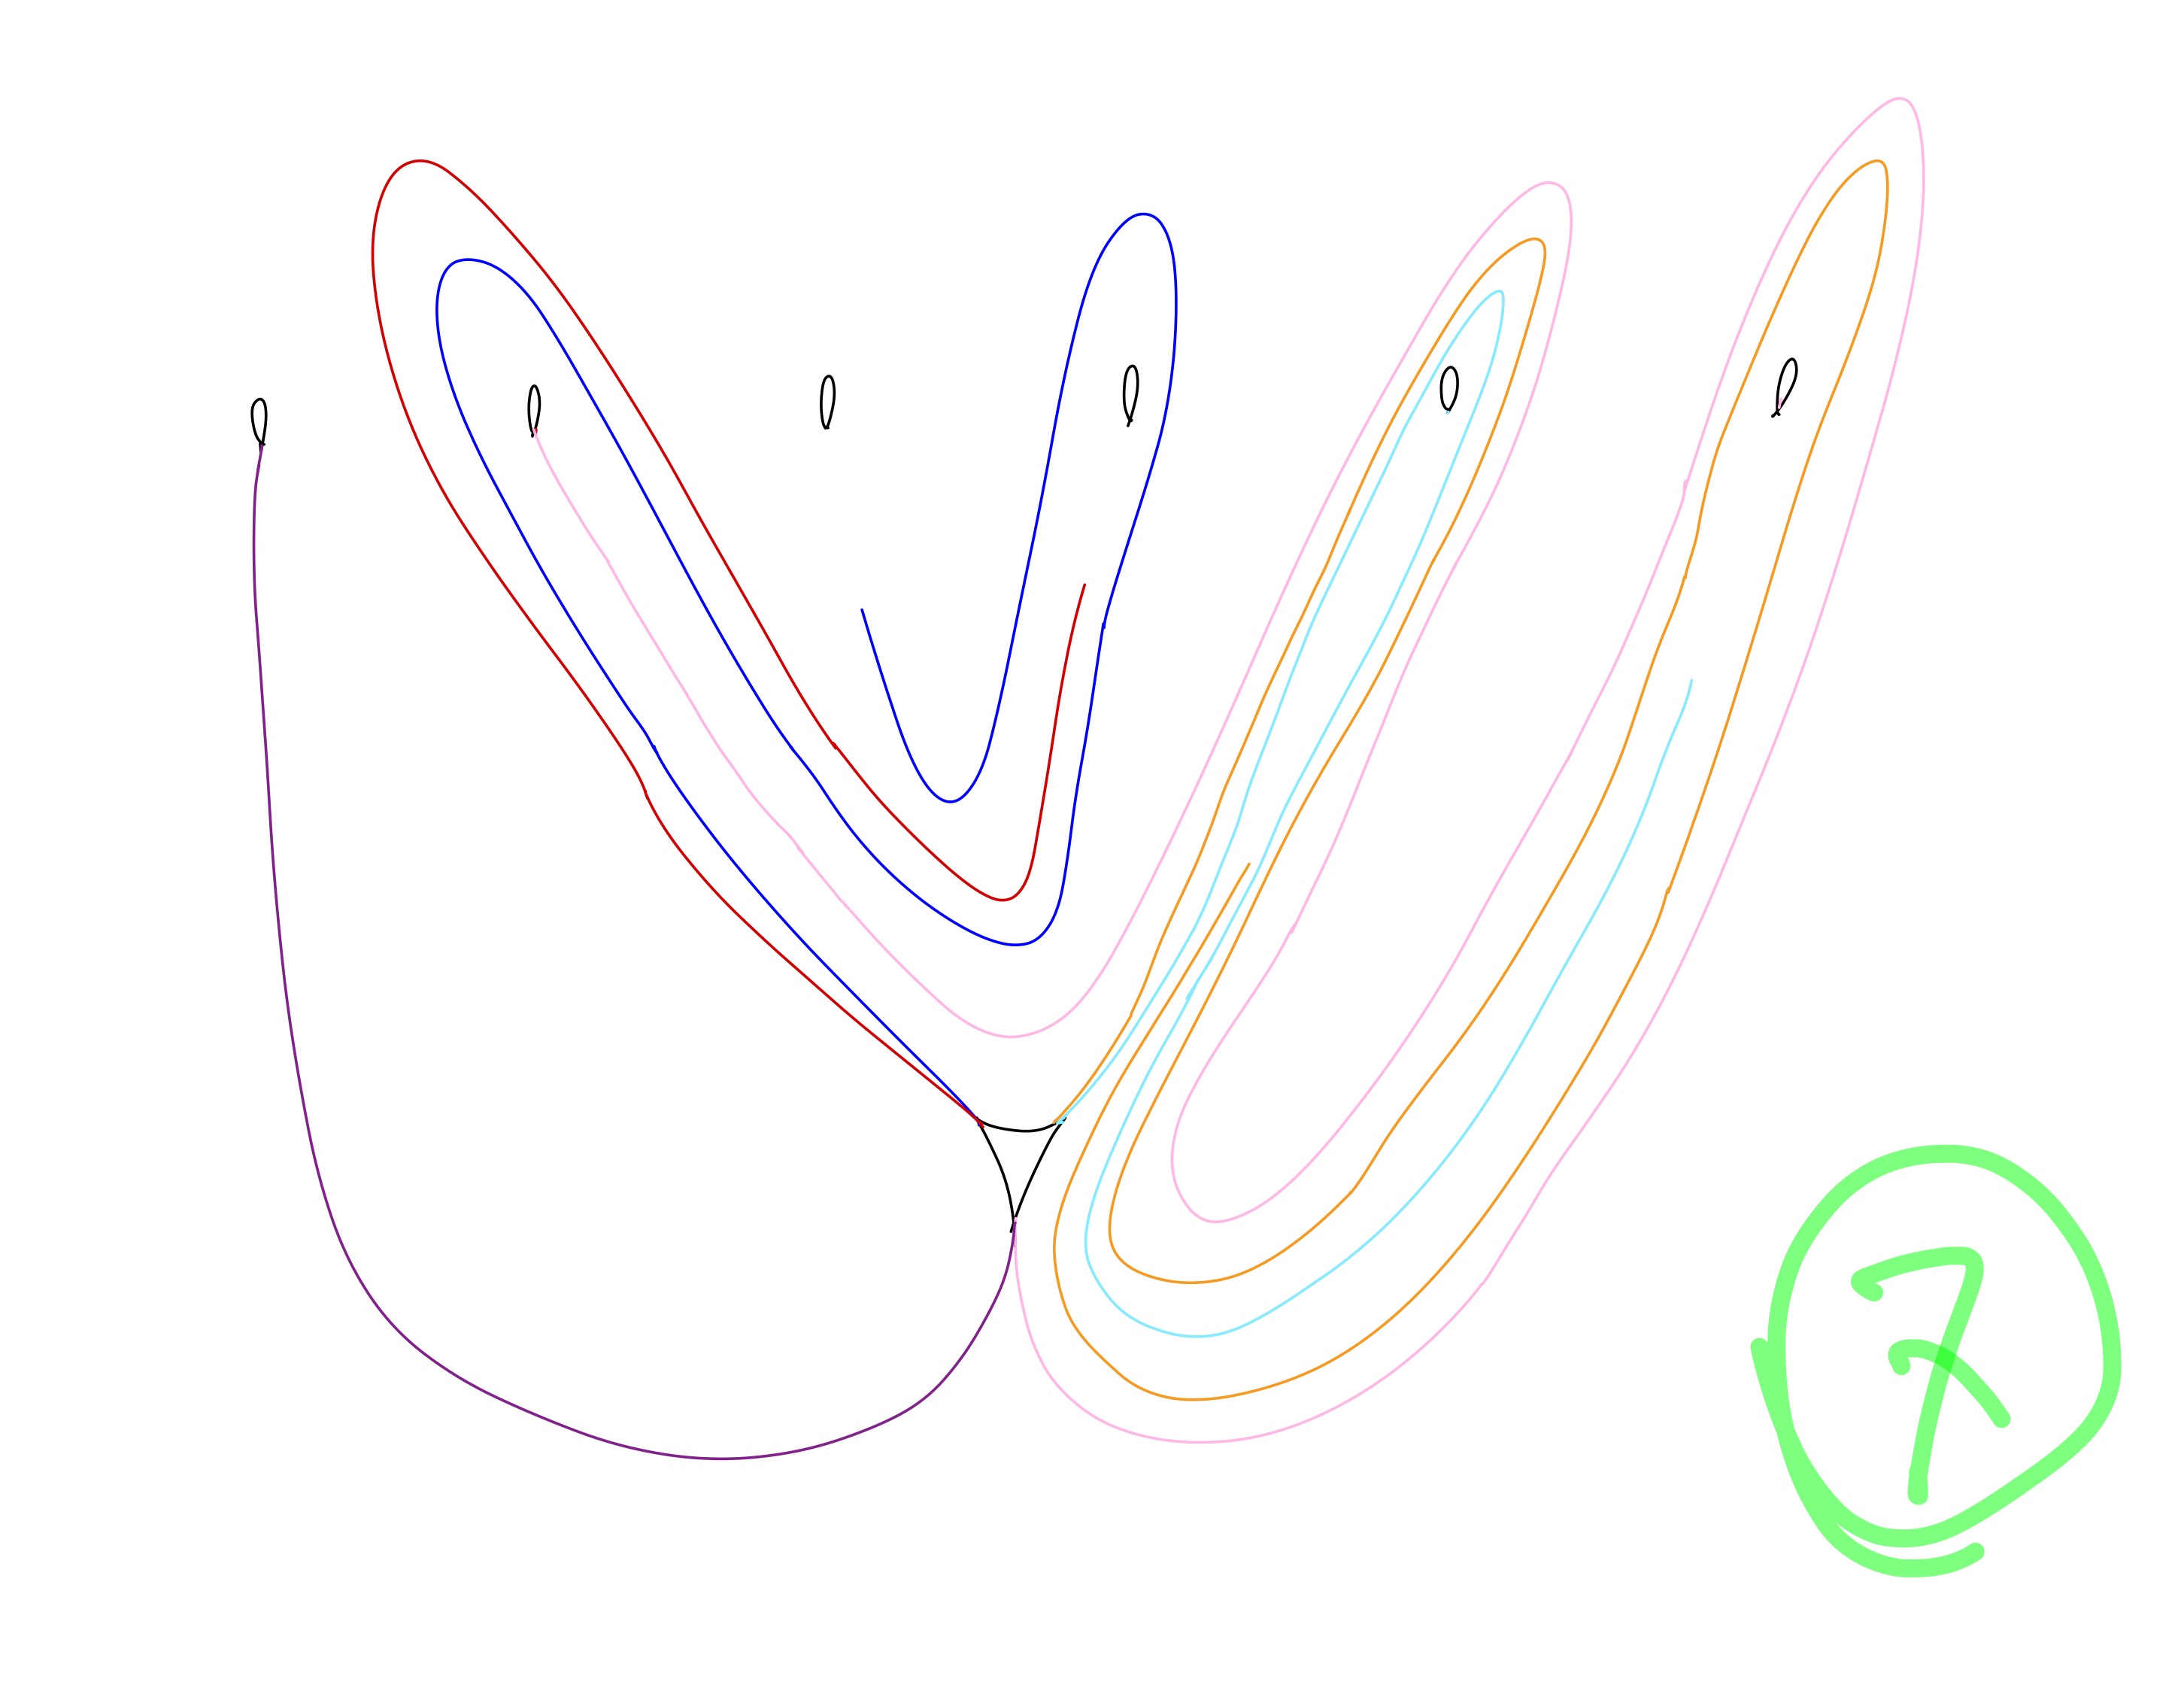
\includegraphics[width=\linewidth, height=0.45\textheight, keepaspectratio]{figures_braid/figures_candelabra/Candelabra Braid 7_Farrago-1.jpg}
    \caption{Train Track Map Candidate Family 7 of the Candelabra.}
    \label{fig:candelabra_braid_b7_map}
\end{figure*}

The inverse of the following braid carries this family of train track maps:
\[
b_7^c = (\sigma_{3}^{-1})^k \sigma_{2} \sigma_{3} \sigma_{4}^{-1} \sigma_{5}^{-1} \sigma_{4}^m \circ G
\]
where $G$ is the braid of Section \ref{sec:braid G}, and $k,m\geq 1$ ($k,m\in \mathbb{Z}$) are the twisting parameters. This is shown in Figure \ref{fig:candelabra_braid_b7}

\begin{figure*}[p]
    \centering
    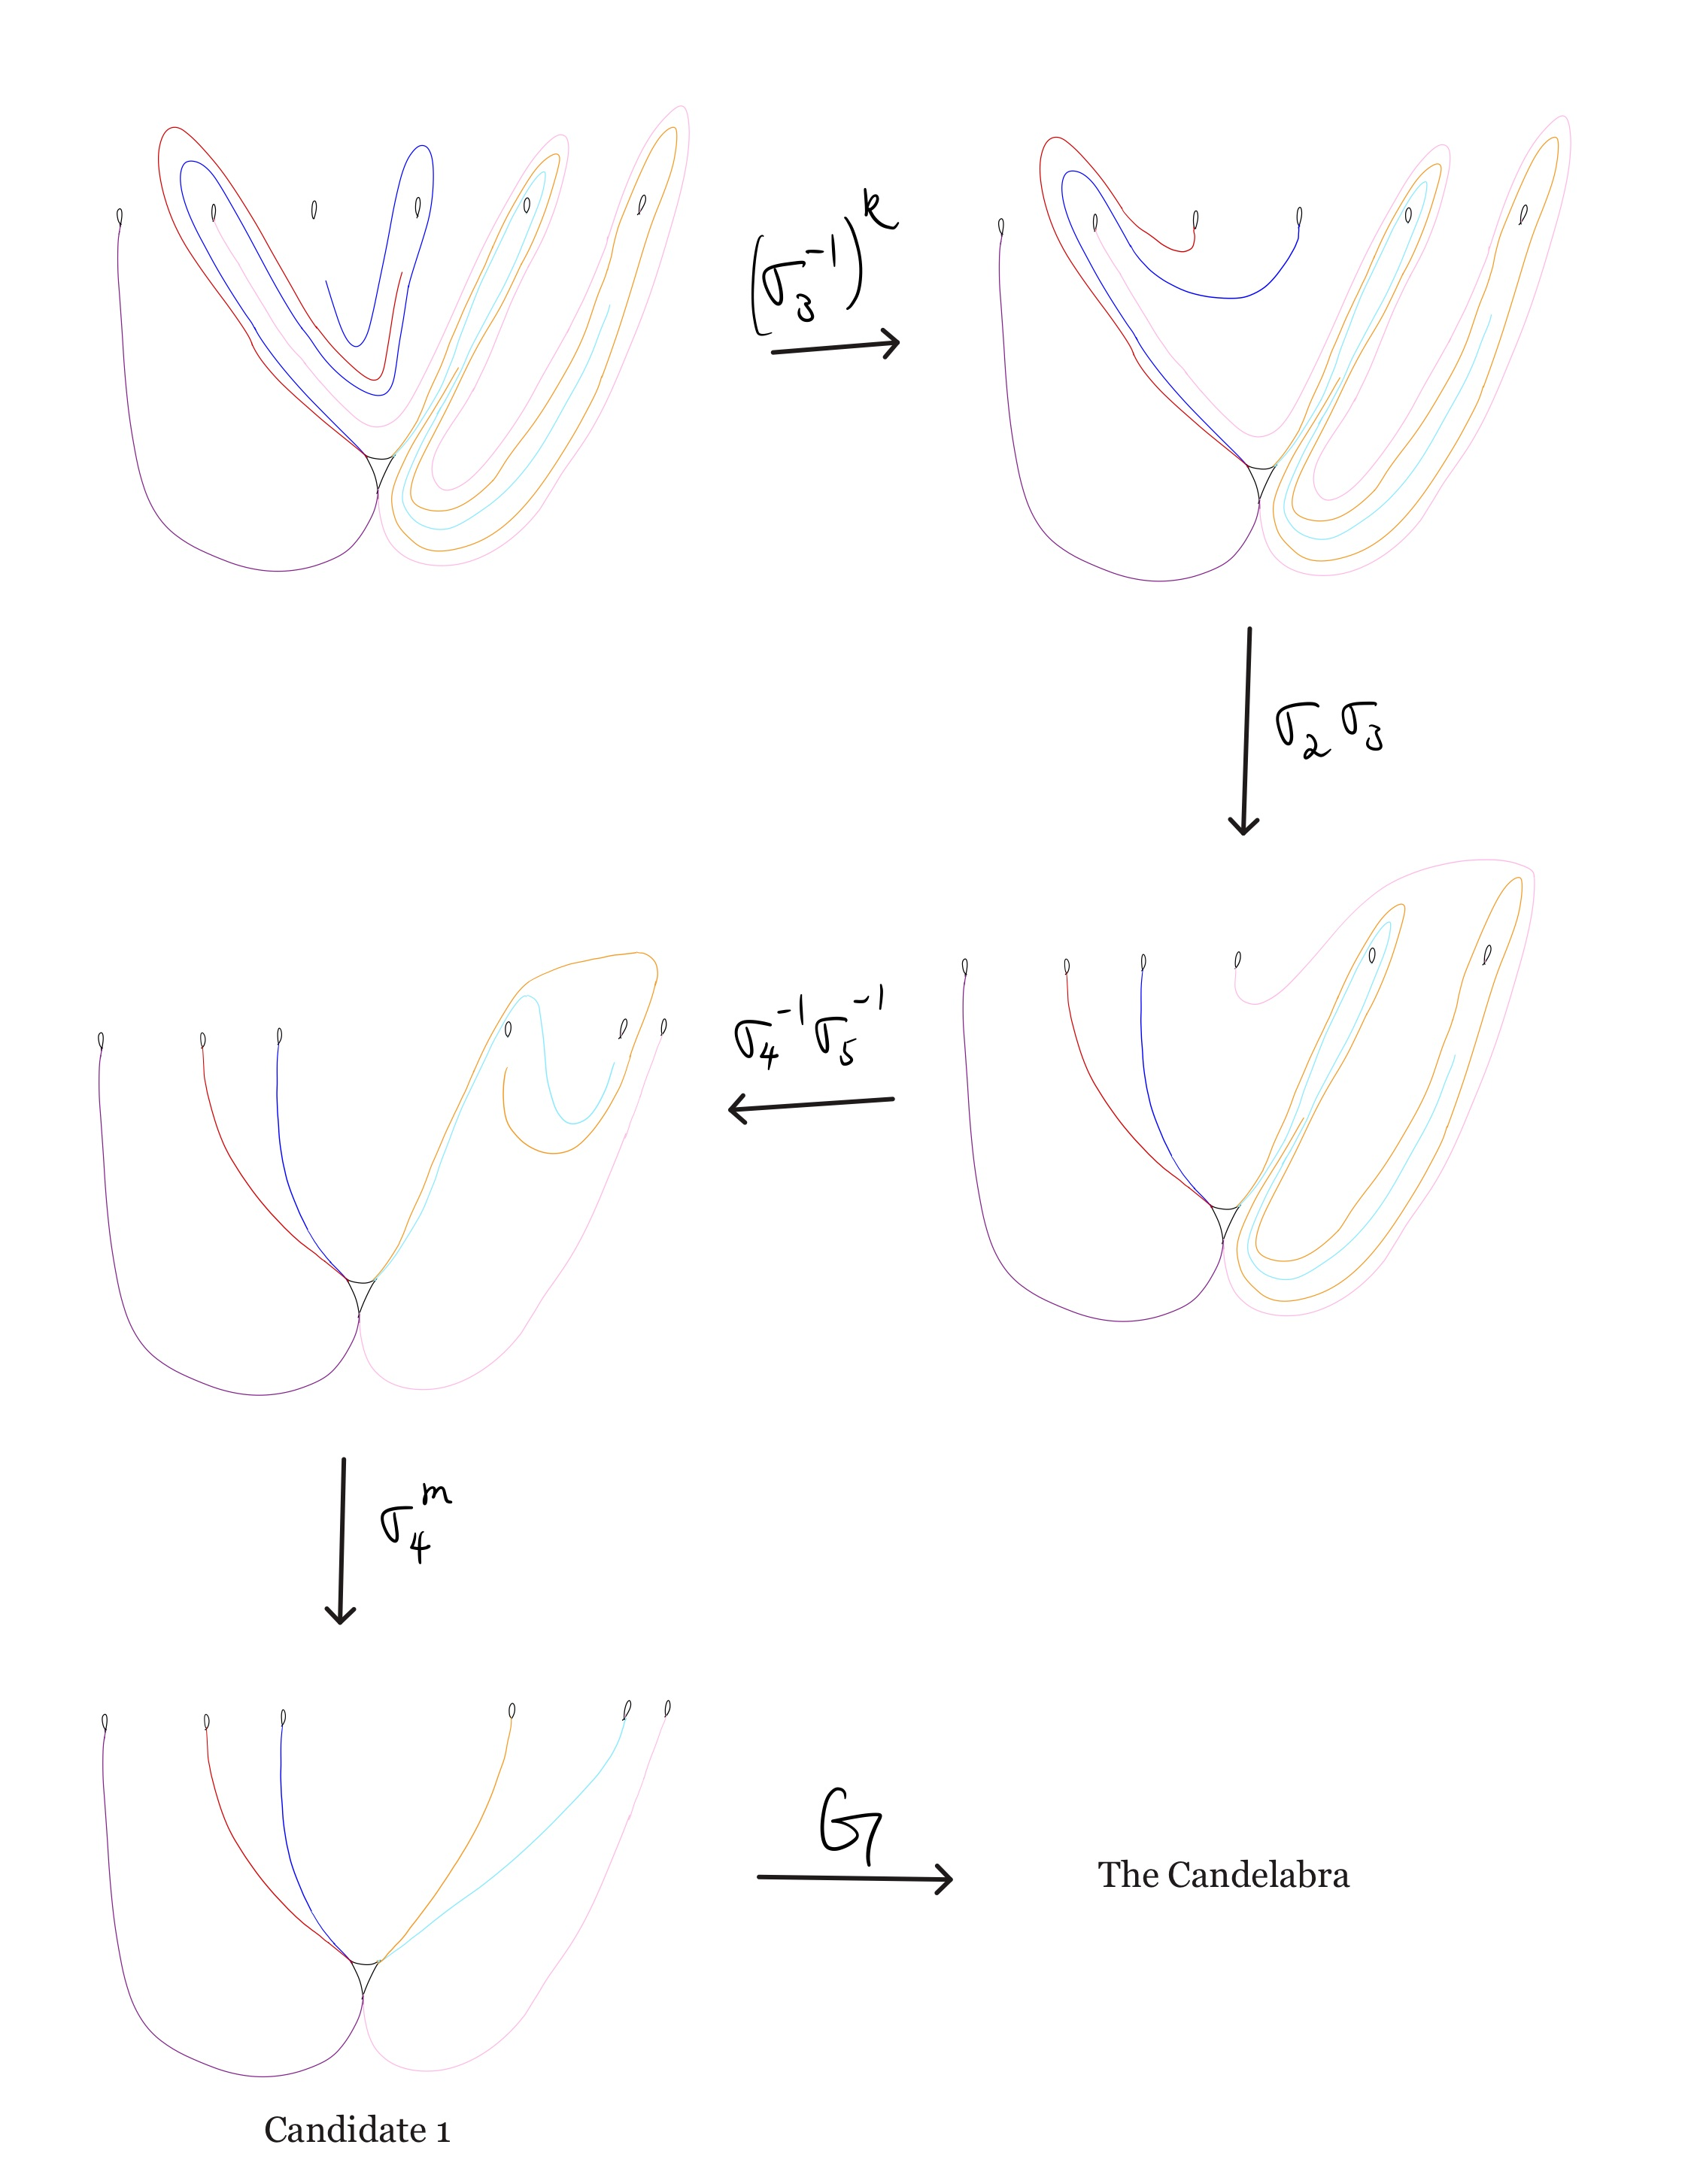
\includegraphics[width=\linewidth, height=0.45\textheight, keepaspectratio]{figures_braid/figures_candelabra/Candelabra Braid 7_Farrago-2.jpg}
    \caption{This sequence shows the inverse of the braid $b_7^c$ carries Train Track Candidate Family 7.}
    \label{fig:candelabra_braid_b7}
\end{figure*}

\clearpage


\section{Candidate Family 8}
Train Track Map Candidate Family 8 of the Candelabra train track is shown in Figure \ref{fig:candelabra_braid_b8_map}. Note there is twisting between $\fbo$ and $\fbs$. See \ref{Jumbuck} for details.

\begin{figure*}[ht]
    \centering
    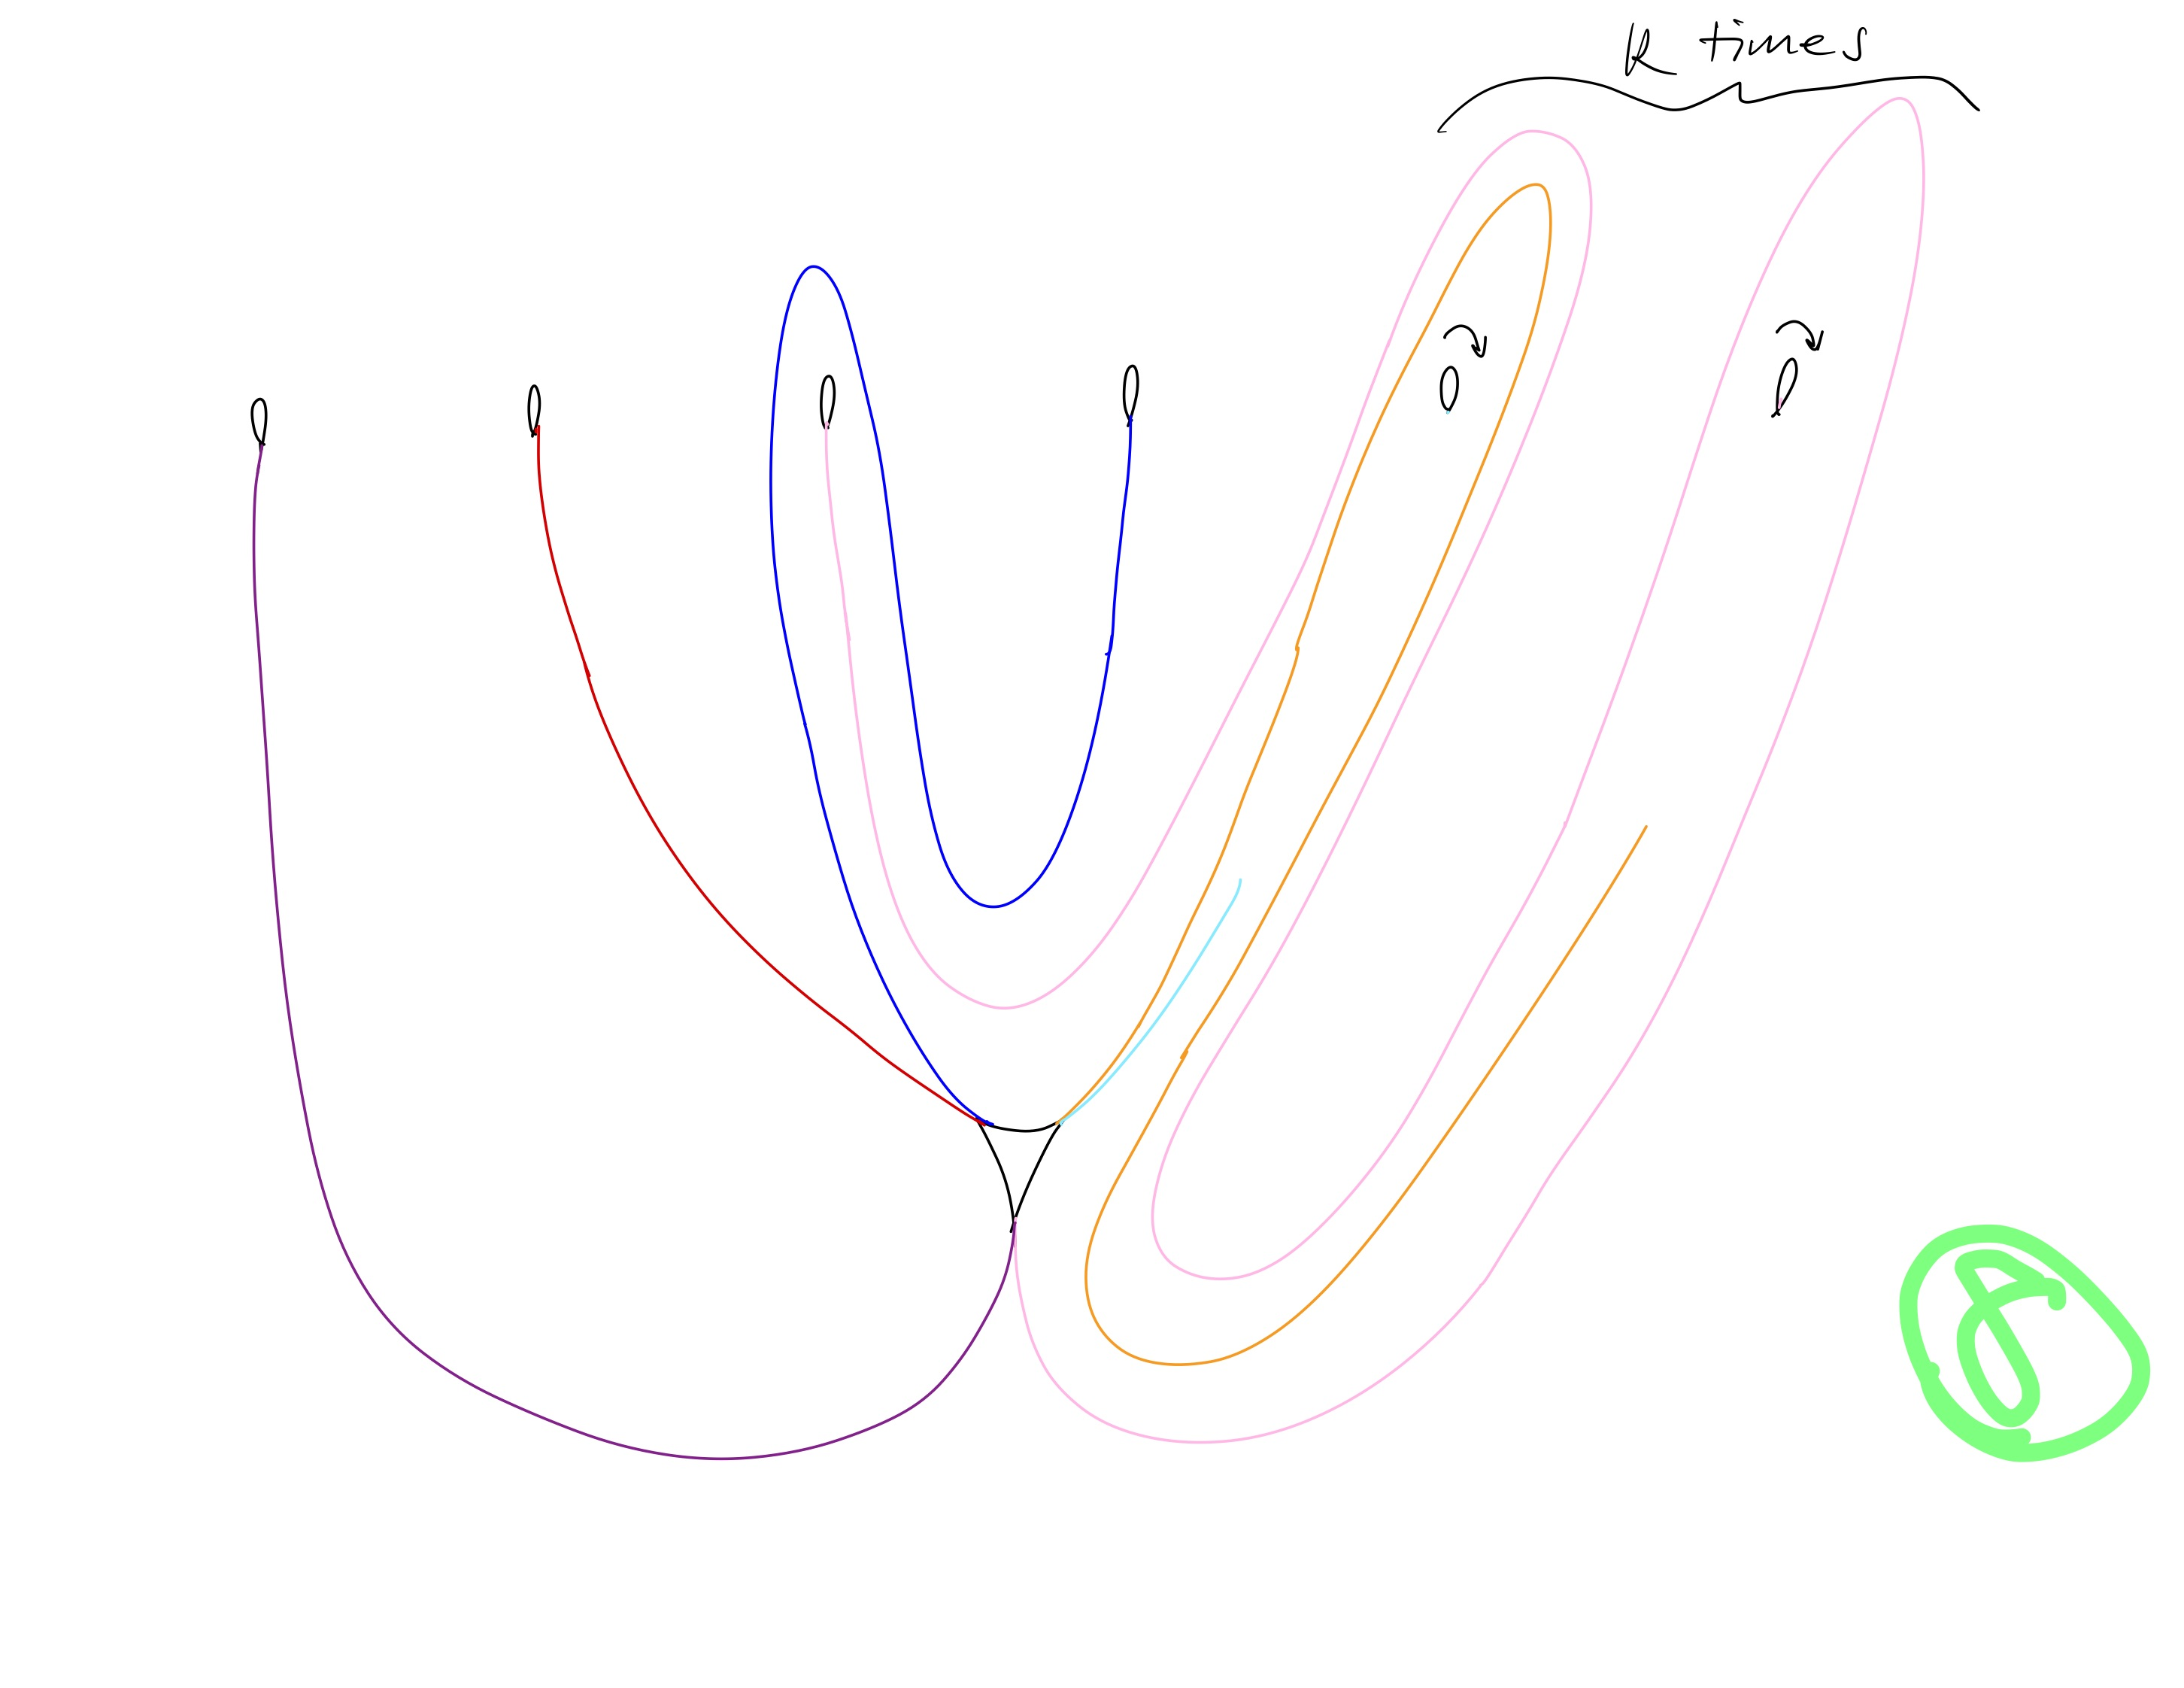
\includegraphics[width=\linewidth, height=0.45\textheight, keepaspectratio]{figures_braid/figures_candelabra/Candelabra Braid 8 Jumbuck-1.jpg}
    \caption{Train Track Map Candidate Family 8 of the Candelabra.}
    \label{fig:candelabra_braid_b8_map}
\end{figure*}

The inverse of the following braid carries this family of train track maps:
\[
b_8^c = \sigma_{5}^k \sigma_{3} \sigma_{4}^{-1} \sigma_{5}^{-1} \circ G
\]
where $G$ is the braid of Section \ref{sec:braid G}, and $k\geq 1$ ($k\in \mathbb{Z}$) is the twisting parameter. This is shown in Figure \ref{fig:candelabra_braid_b8}

\begin{figure*}[p]
    \centering
    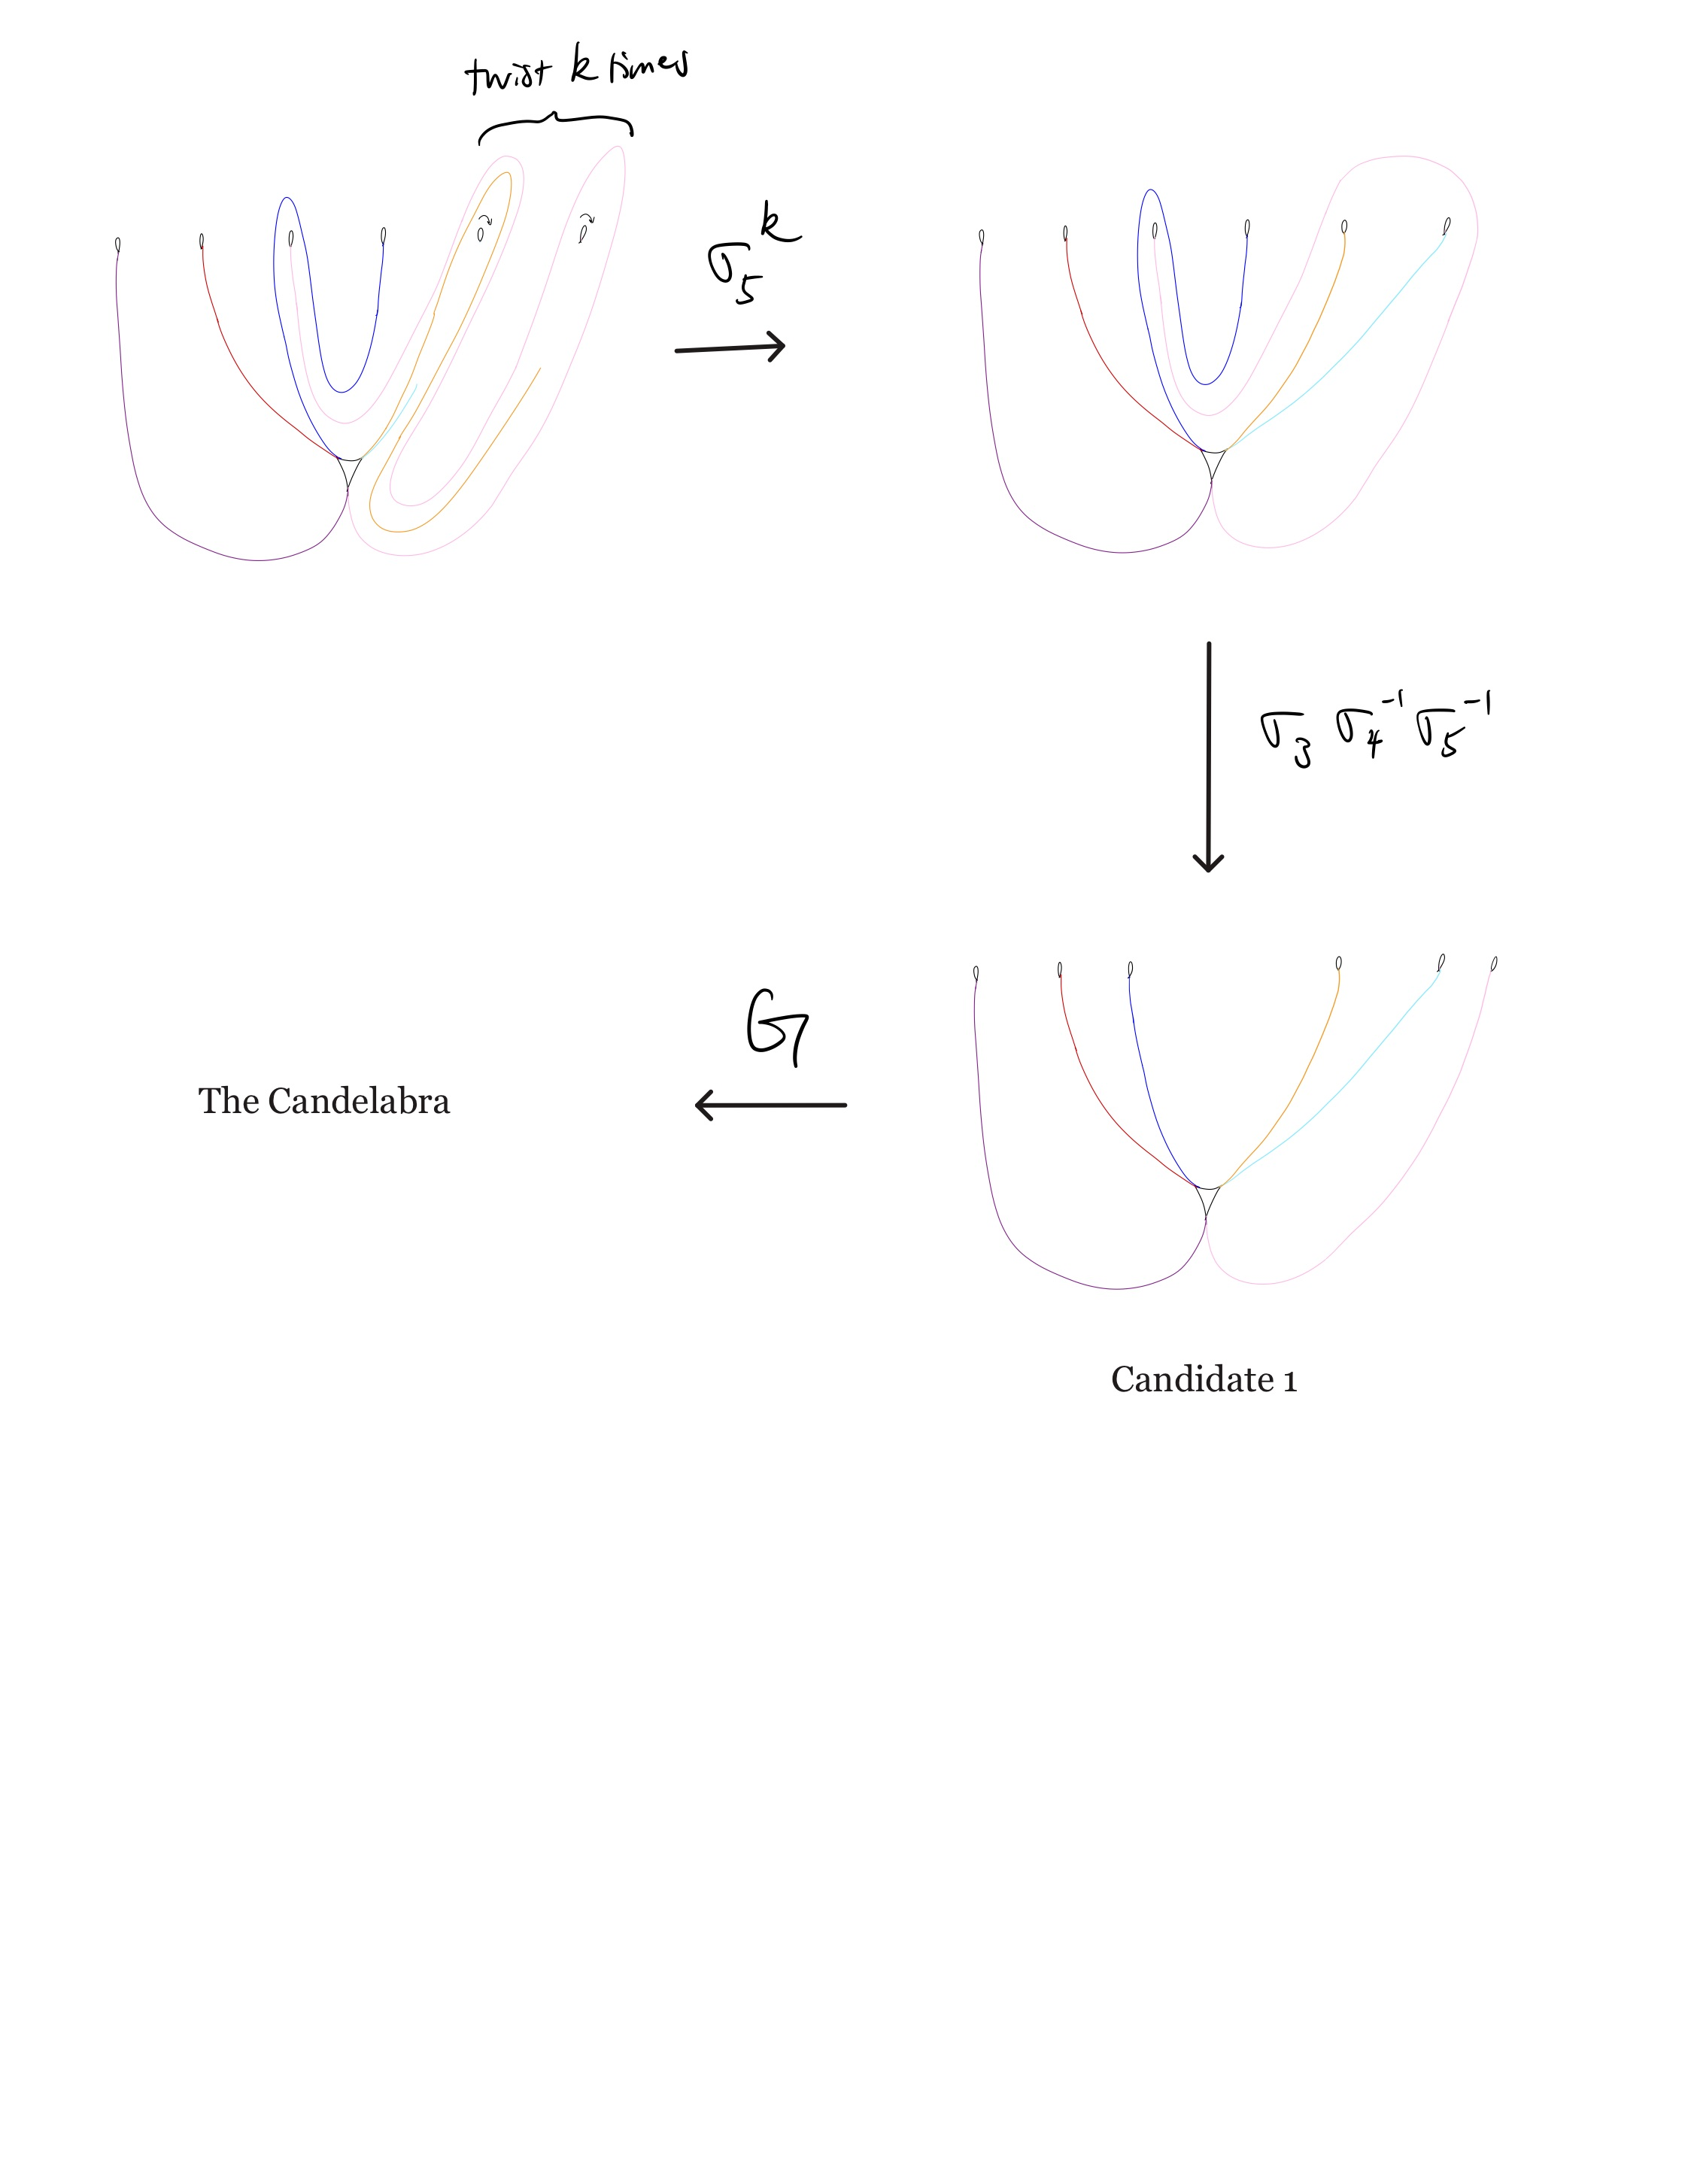
\includegraphics[width=\linewidth, height=0.45\textheight, keepaspectratio]{figures_braid/figures_candelabra/Candelabra Braid 8 Jumbuck-2.jpg}
    \caption{This sequence shows the inverse of the braid $b_8^c$ carries Train Track Candidate Family 8.}
    \label{fig:candelabra_braid_b8}
\end{figure*}

\clearpage


\section{Candidate Family 9}
Train Track Map Candidate Family 9 of the Candelabra train track is shown in Figure \ref{fig:candelabra_braid_b9_map}. Note there is twisting among $\fbi$, $\fbo$ and $\fbs$. See \ref{Nithing} for details.

\begin{figure*}[ht]
    \centering
    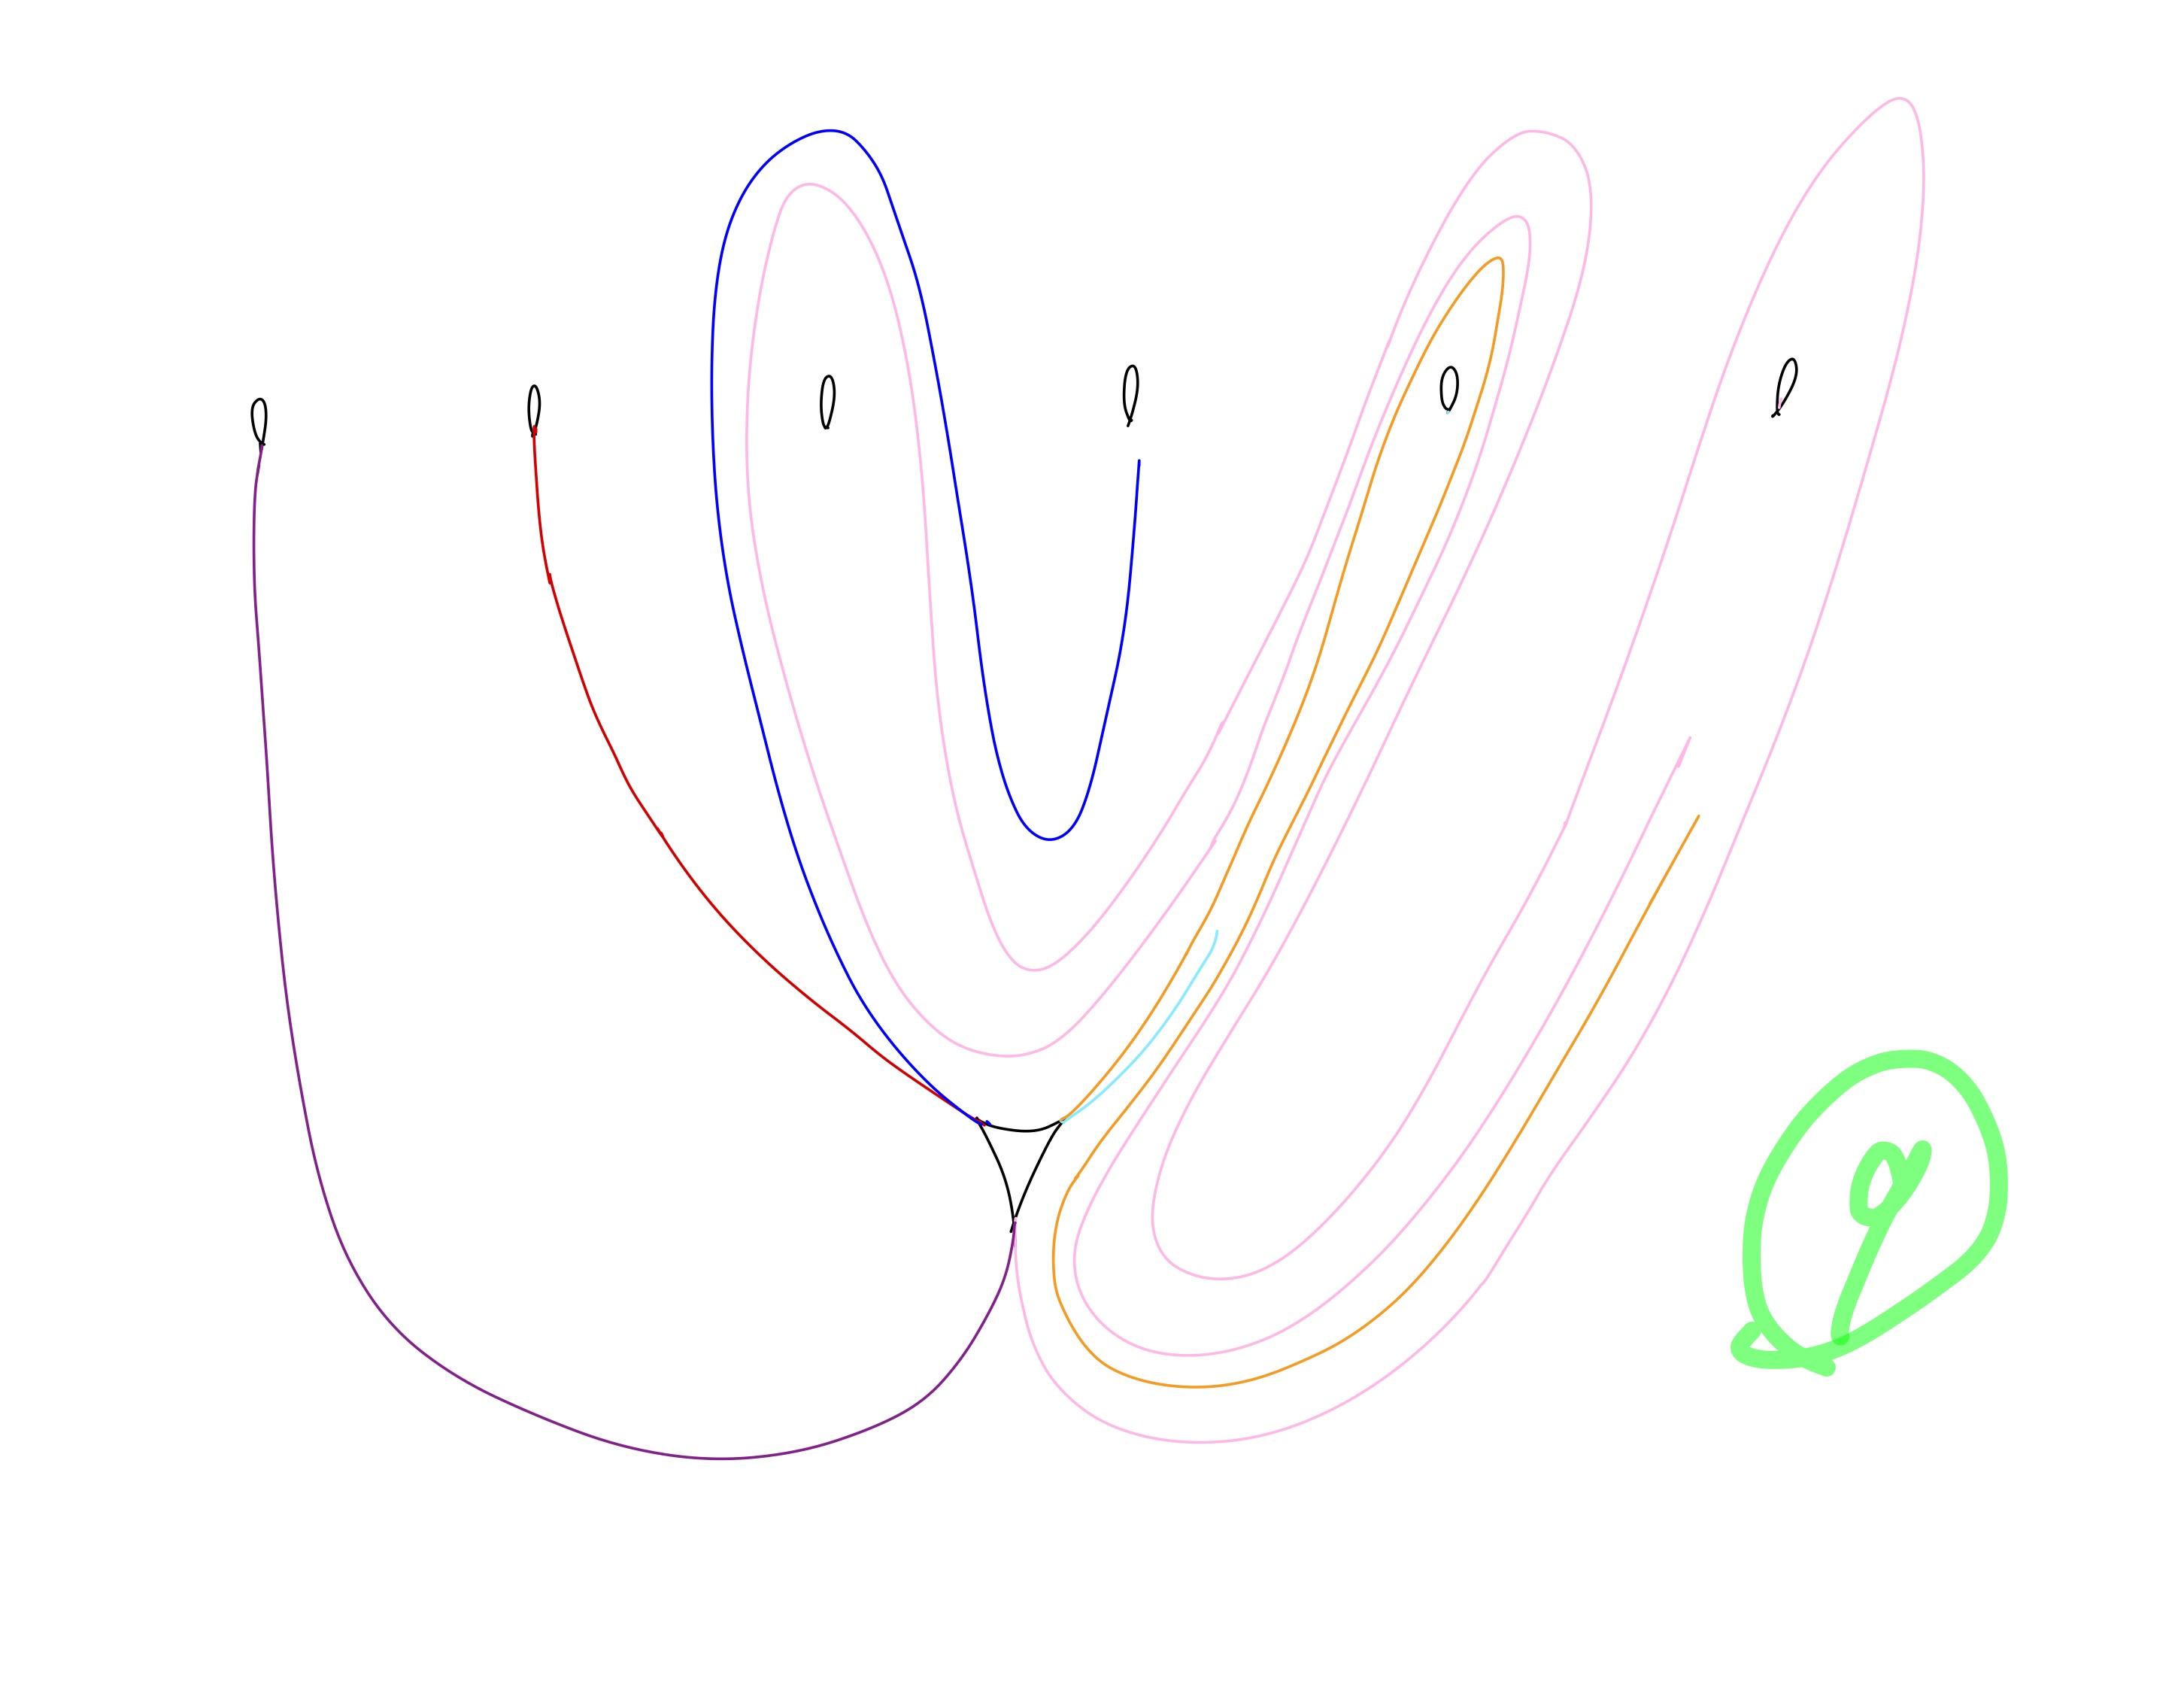
\includegraphics[width=\linewidth, height=0.45\textheight, keepaspectratio]{figures_braid/figures_candelabra/Candelabra Braid 9 Nithing-1.jpg}
    \caption{Train Track Map Candidate Family 9 of the Candelabra.}
    \label{fig:candelabra_braid_b9_map}
\end{figure*}

The inverse of the following braid carries this family of train track maps:
\[
b_9^c = \sigma_{5}^m \sigma_{3} (\sigma_{4}^{-1})^k \sigma_{4}^{-1} \sigma_{5}^{-1} \circ G
\]
where $G$ is the braid of Section \ref{sec:braid G}, and $k,m\geq 1$ ($k,m\in \mathbb{Z}$) are the twisting parameters. This is shown in Figure \ref{fig:candelabra_braid_b9}

\begin{figure*}[p]
    \centering
    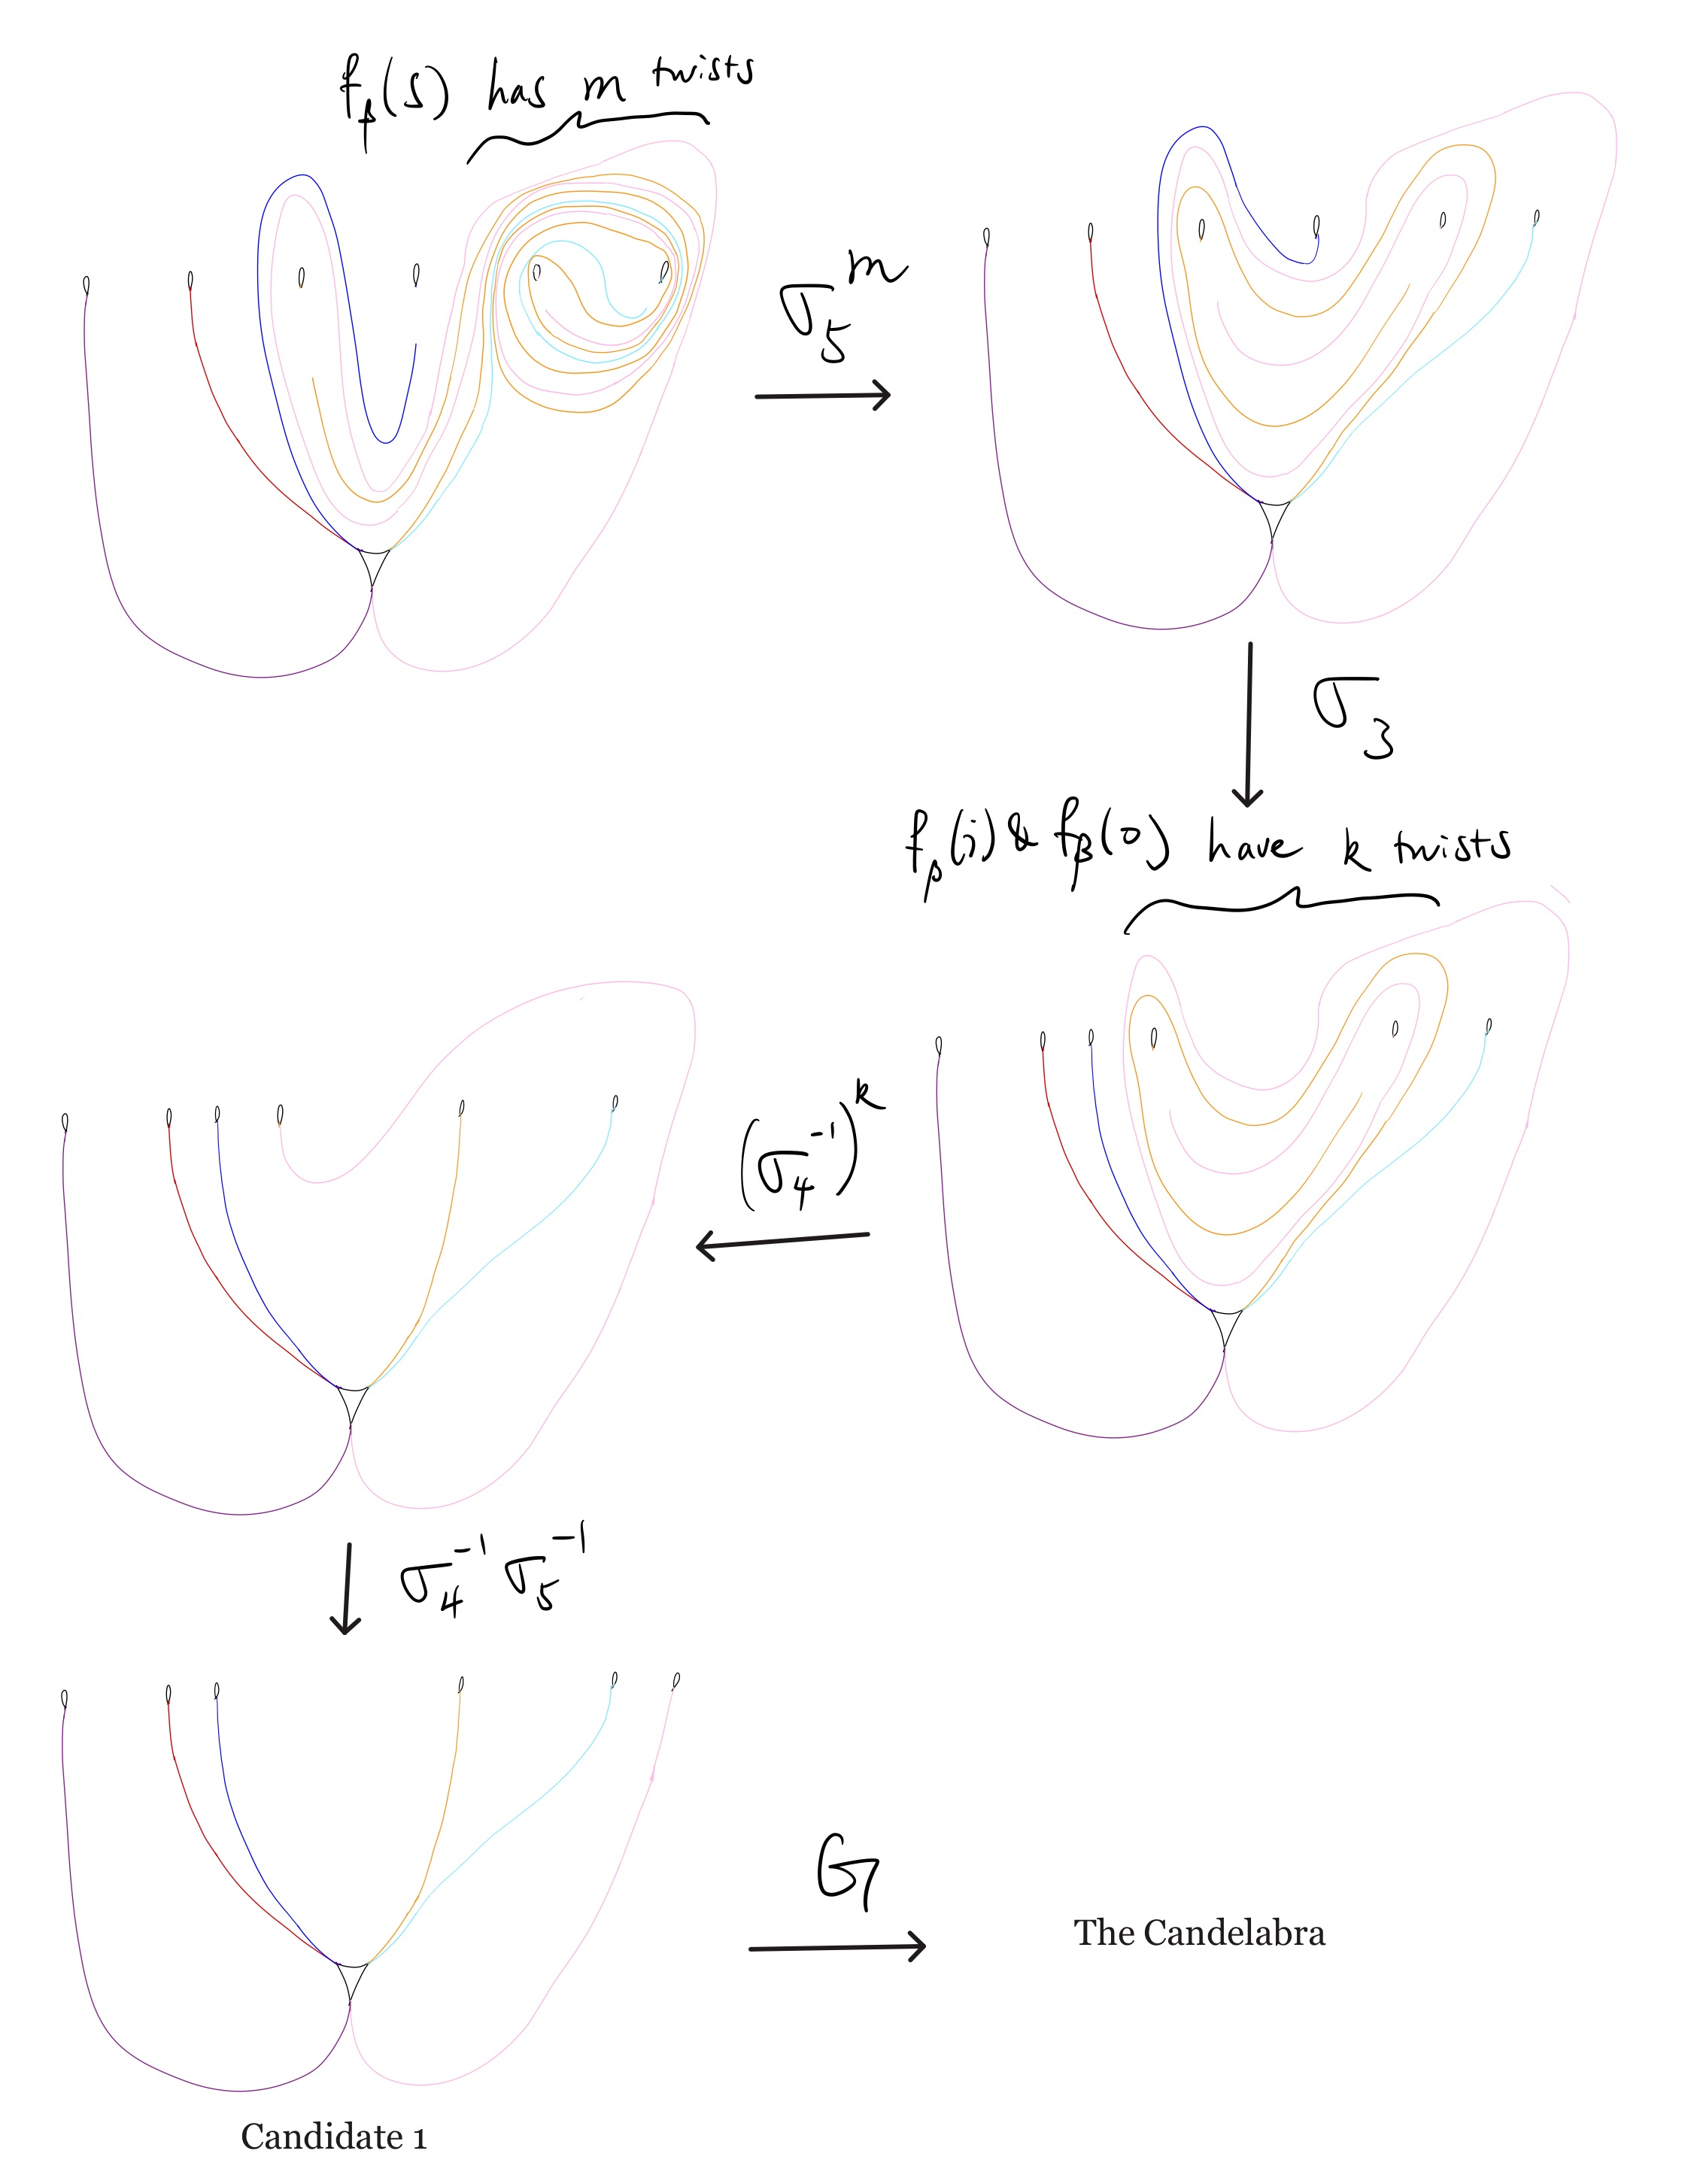
\includegraphics[width=\linewidth, height=0.45\textheight, keepaspectratio]{figures_braid/figures_candelabra/Candelabra Braid 9 Nithing-2.jpg}
    \caption{This sequence shows the inverse of the braid $b_9^c$ carries Train Track Candidate Family 9.}
    \label{fig:candelabra_braid_b9}
\end{figure*}

\clearpage

\section{Candidate Family 10}
Train Track Map Candidate Family 10 of the Candelabra train track is shown in Figure \ref{fig:candelabra_braid_b10_map}. Note there is twisting between $\fbo$ and $\fbs$. See \ref{Chouse} for details.

\begin{figure*}[ht]
    \centering
    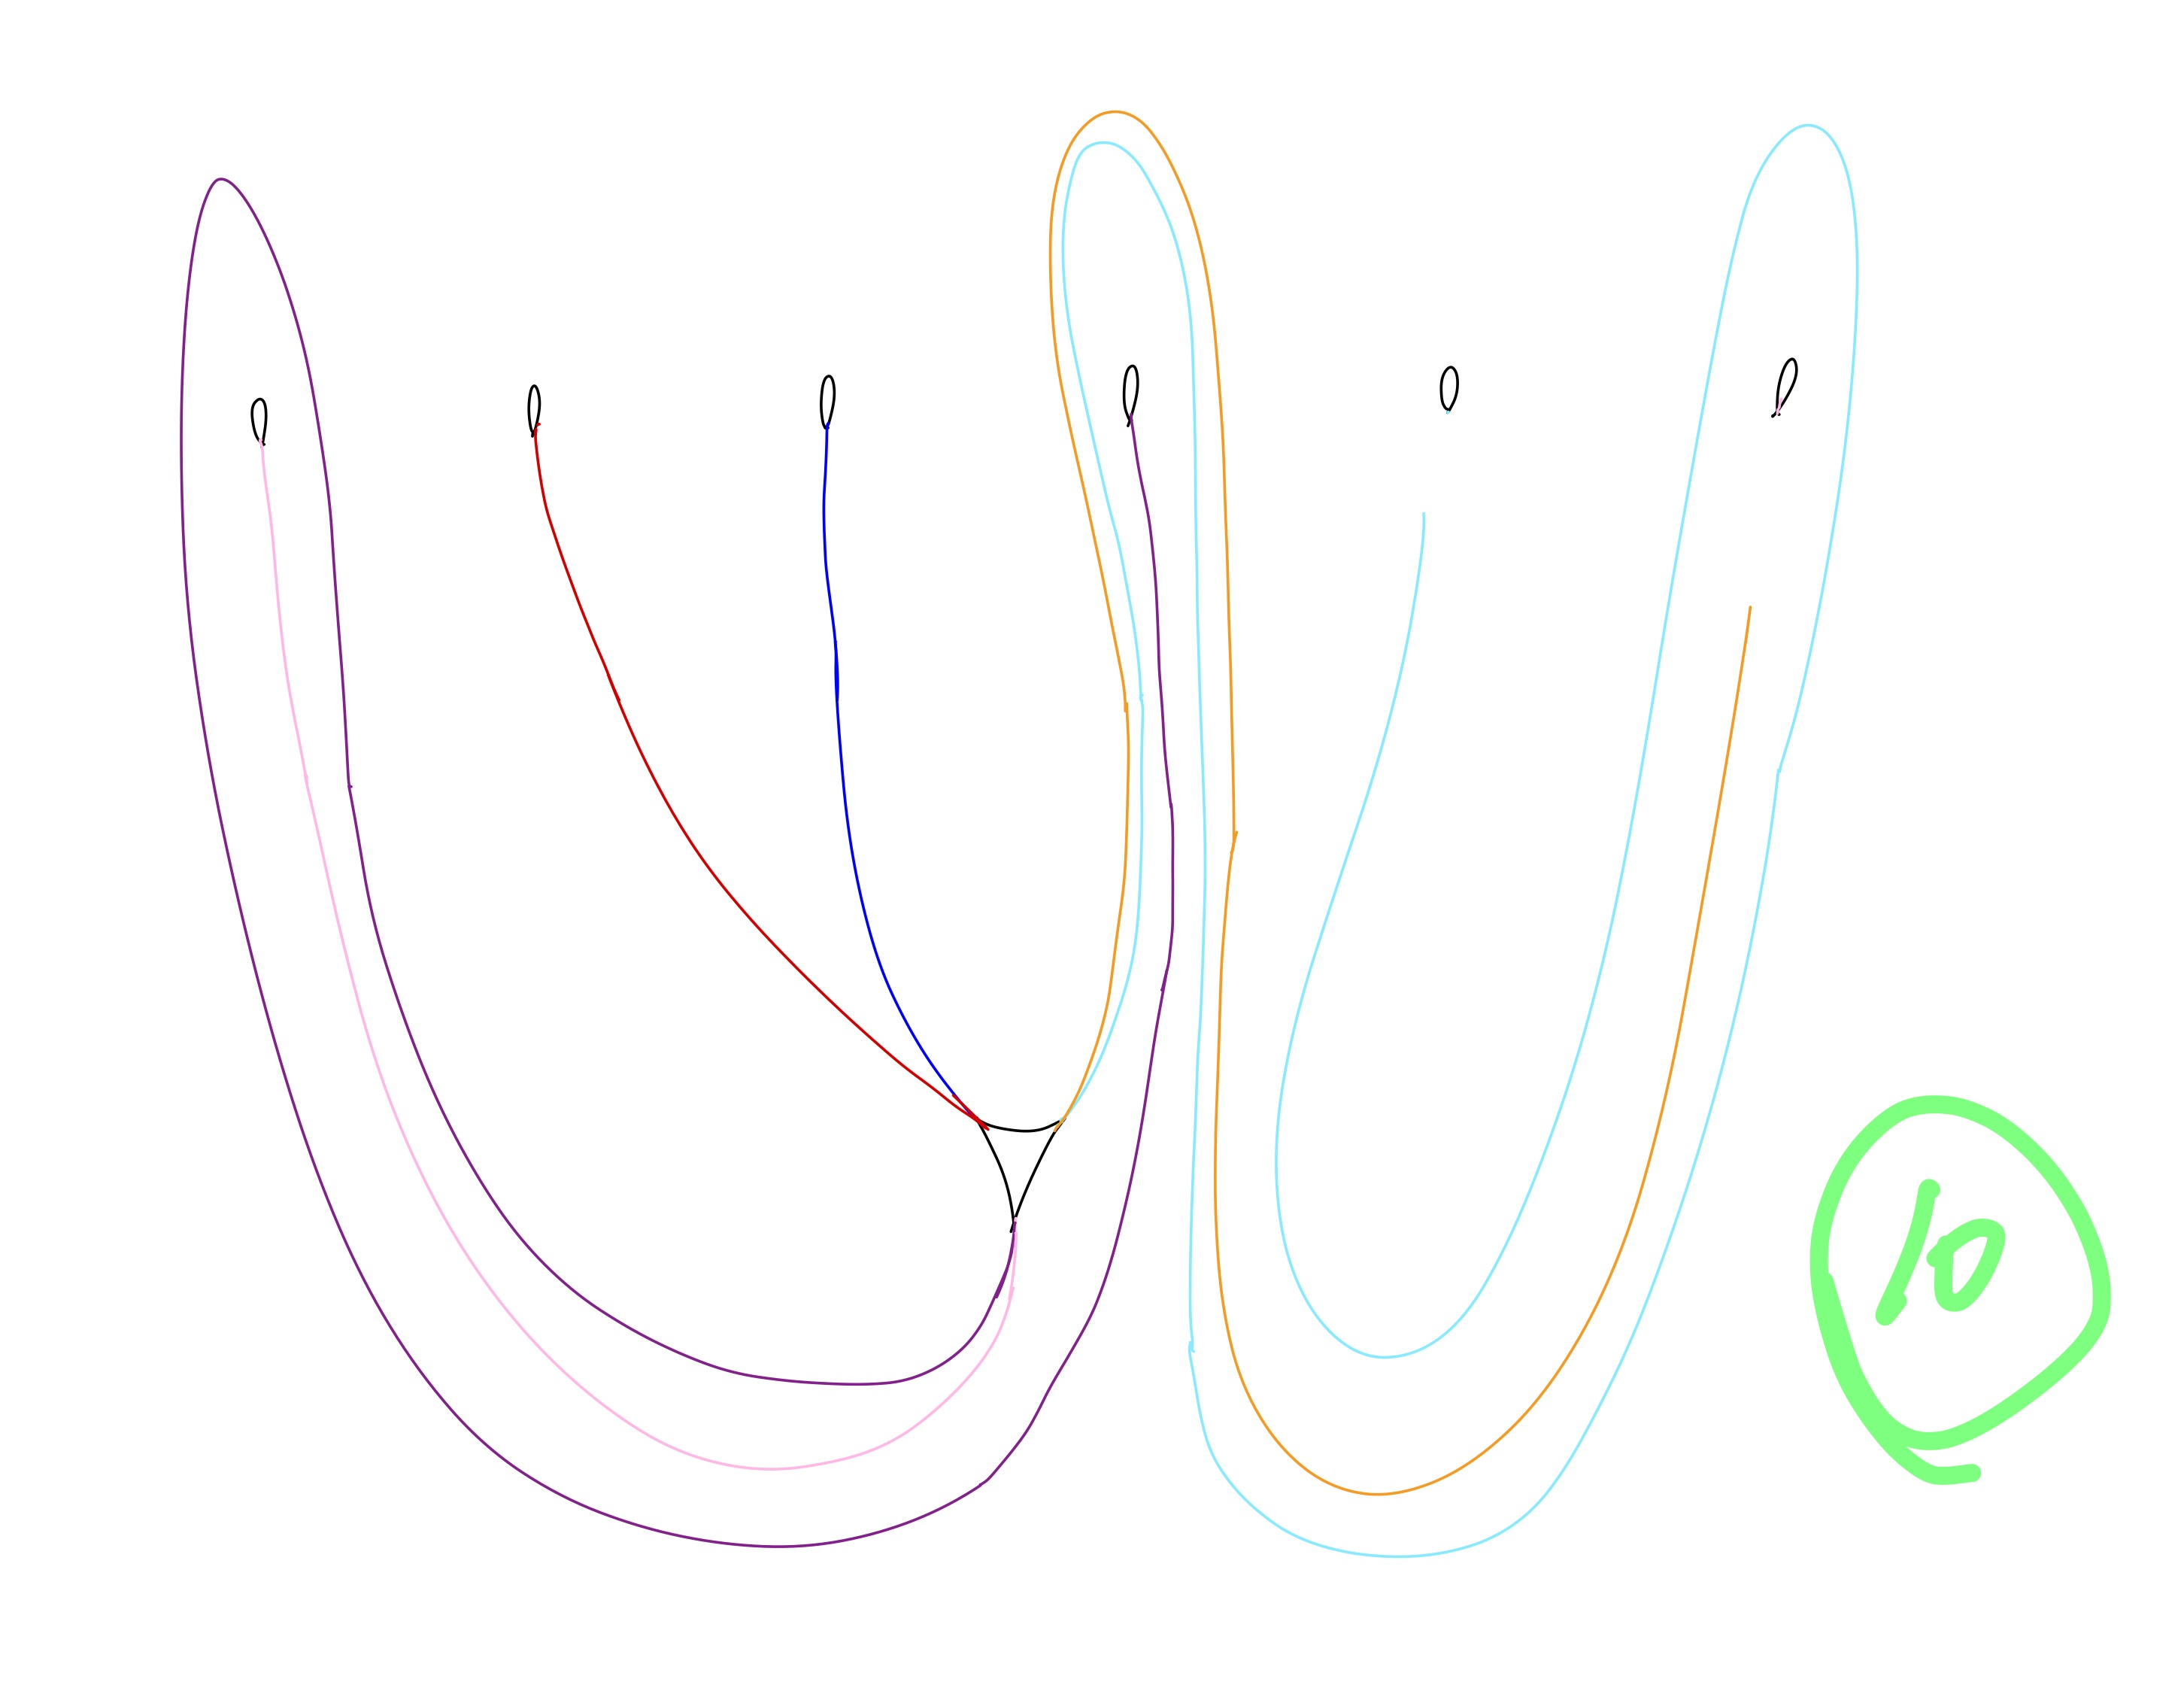
\includegraphics[width=\linewidth, height=0.45\textheight, keepaspectratio]{figures_braid/figures_candelabra/Candelabra Braid 10 Chouse-1.jpg}
    \caption{Train Track Map Candidate Family 10 of the Candelabra.}
    \label{fig:candelabra_braid_b10_map}
\end{figure*}

For this and subsequent candidates, we define the auxiliary braid $F$:
\begin{flushleft}
$\displaystyle F = \allowbreak\sigma_{5}\allowbreak\sigma_{4}\allowbreak\sigma_{3}\allowbreak\sigma_{2}\allowbreak\sigma_{1}\allowbreak\sigma_{2}\allowbreak\sigma_{3}\allowbreak\sigma_{4}\allowbreak\sigma_{5}\allowbreak\sigma_{5}\allowbreak\sigma_{4}\allowbreak\sigma_{3}\allowbreak\sigma_{2}\allowbreak\sigma_{3}\allowbreak\sigma_{4}\allowbreak\sigma_{5}\allowbreak\sigma_{5}\allowbreak\sigma_{4}\allowbreak\sigma_{3}\allowbreak\sigma_{4}\allowbreak\sigma_{5}\allowbreak\sigma_{5}\allowbreak\sigma_{4}\allowbreak\sigma_{5}\allowbreak\sigma_{5}$
\end{flushleft}

The inverse of the following braid carries this family of train track maps:
\[
b_{10}^c = (\sigma_{5}^{-1})^k \sigma_{4} \sigma_{5} \sigma_{1} \sigma_{2} \sigma_{3} \sigma_{4} \circ F \circ G
\]
where $G$ is the braid of Section \ref{sec:braid G}, and $k\geq 1$ ($k\in \mathbb{Z}$) is the twisting parameter. This is shown in Figure \ref{fig:candelabra_braid_b10}.

\begin{figure*}[p]
    \centering
    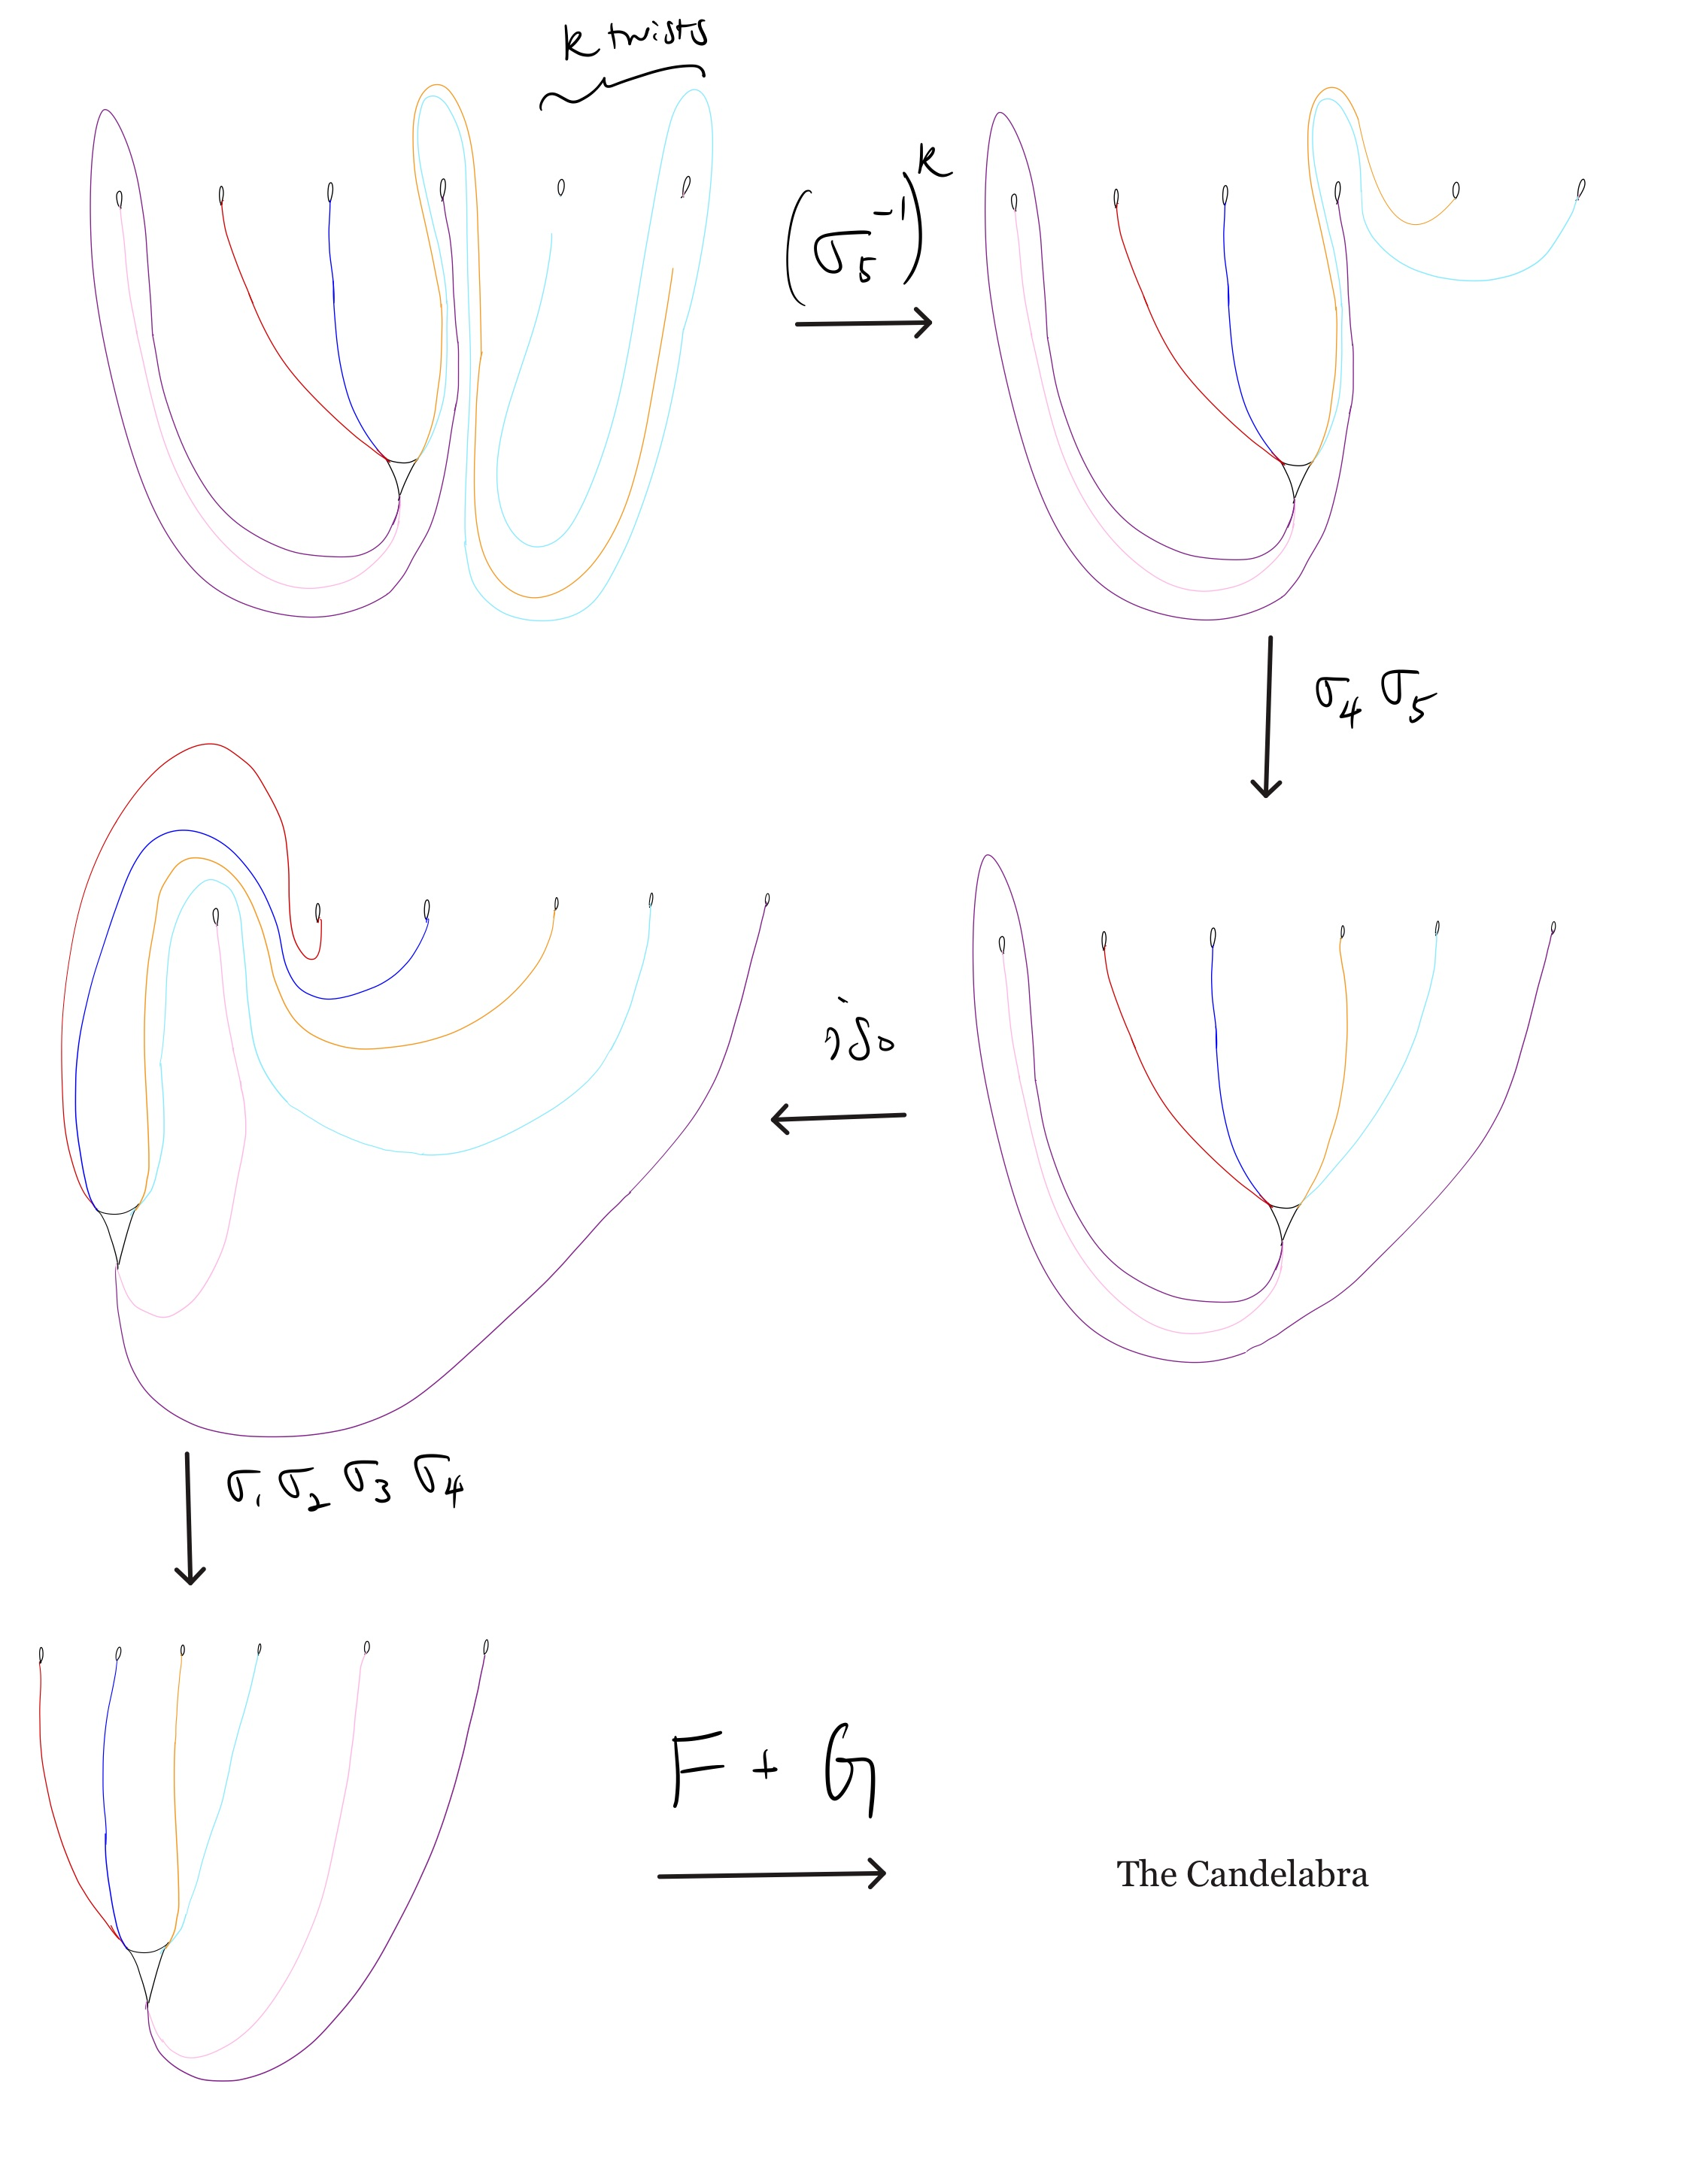
\includegraphics[width=\linewidth, height=0.45\textheight, keepaspectratio]{figures_braid/figures_candelabra/Candelabra Braid 10 Chouse-2.jpg}
    \caption{This sequence shows the inverse of the braid $b_{10}^c$ carries Train Track Candidate Family 10.}
    \label{fig:candelabra_braid_b10}
\end{figure*}

\clearpage

\section{Candidate Family 11}
Train Track Map Candidate Family 11 of the Candelabra train track is shown in Figure \ref{fig:candelabra_braid_b11_map}. Note there is twisting among $\fbp$, $\fbo$ and $\fbs$. See \ref{Fardel} for details.

\begin{figure*}[ht]
    \centering
    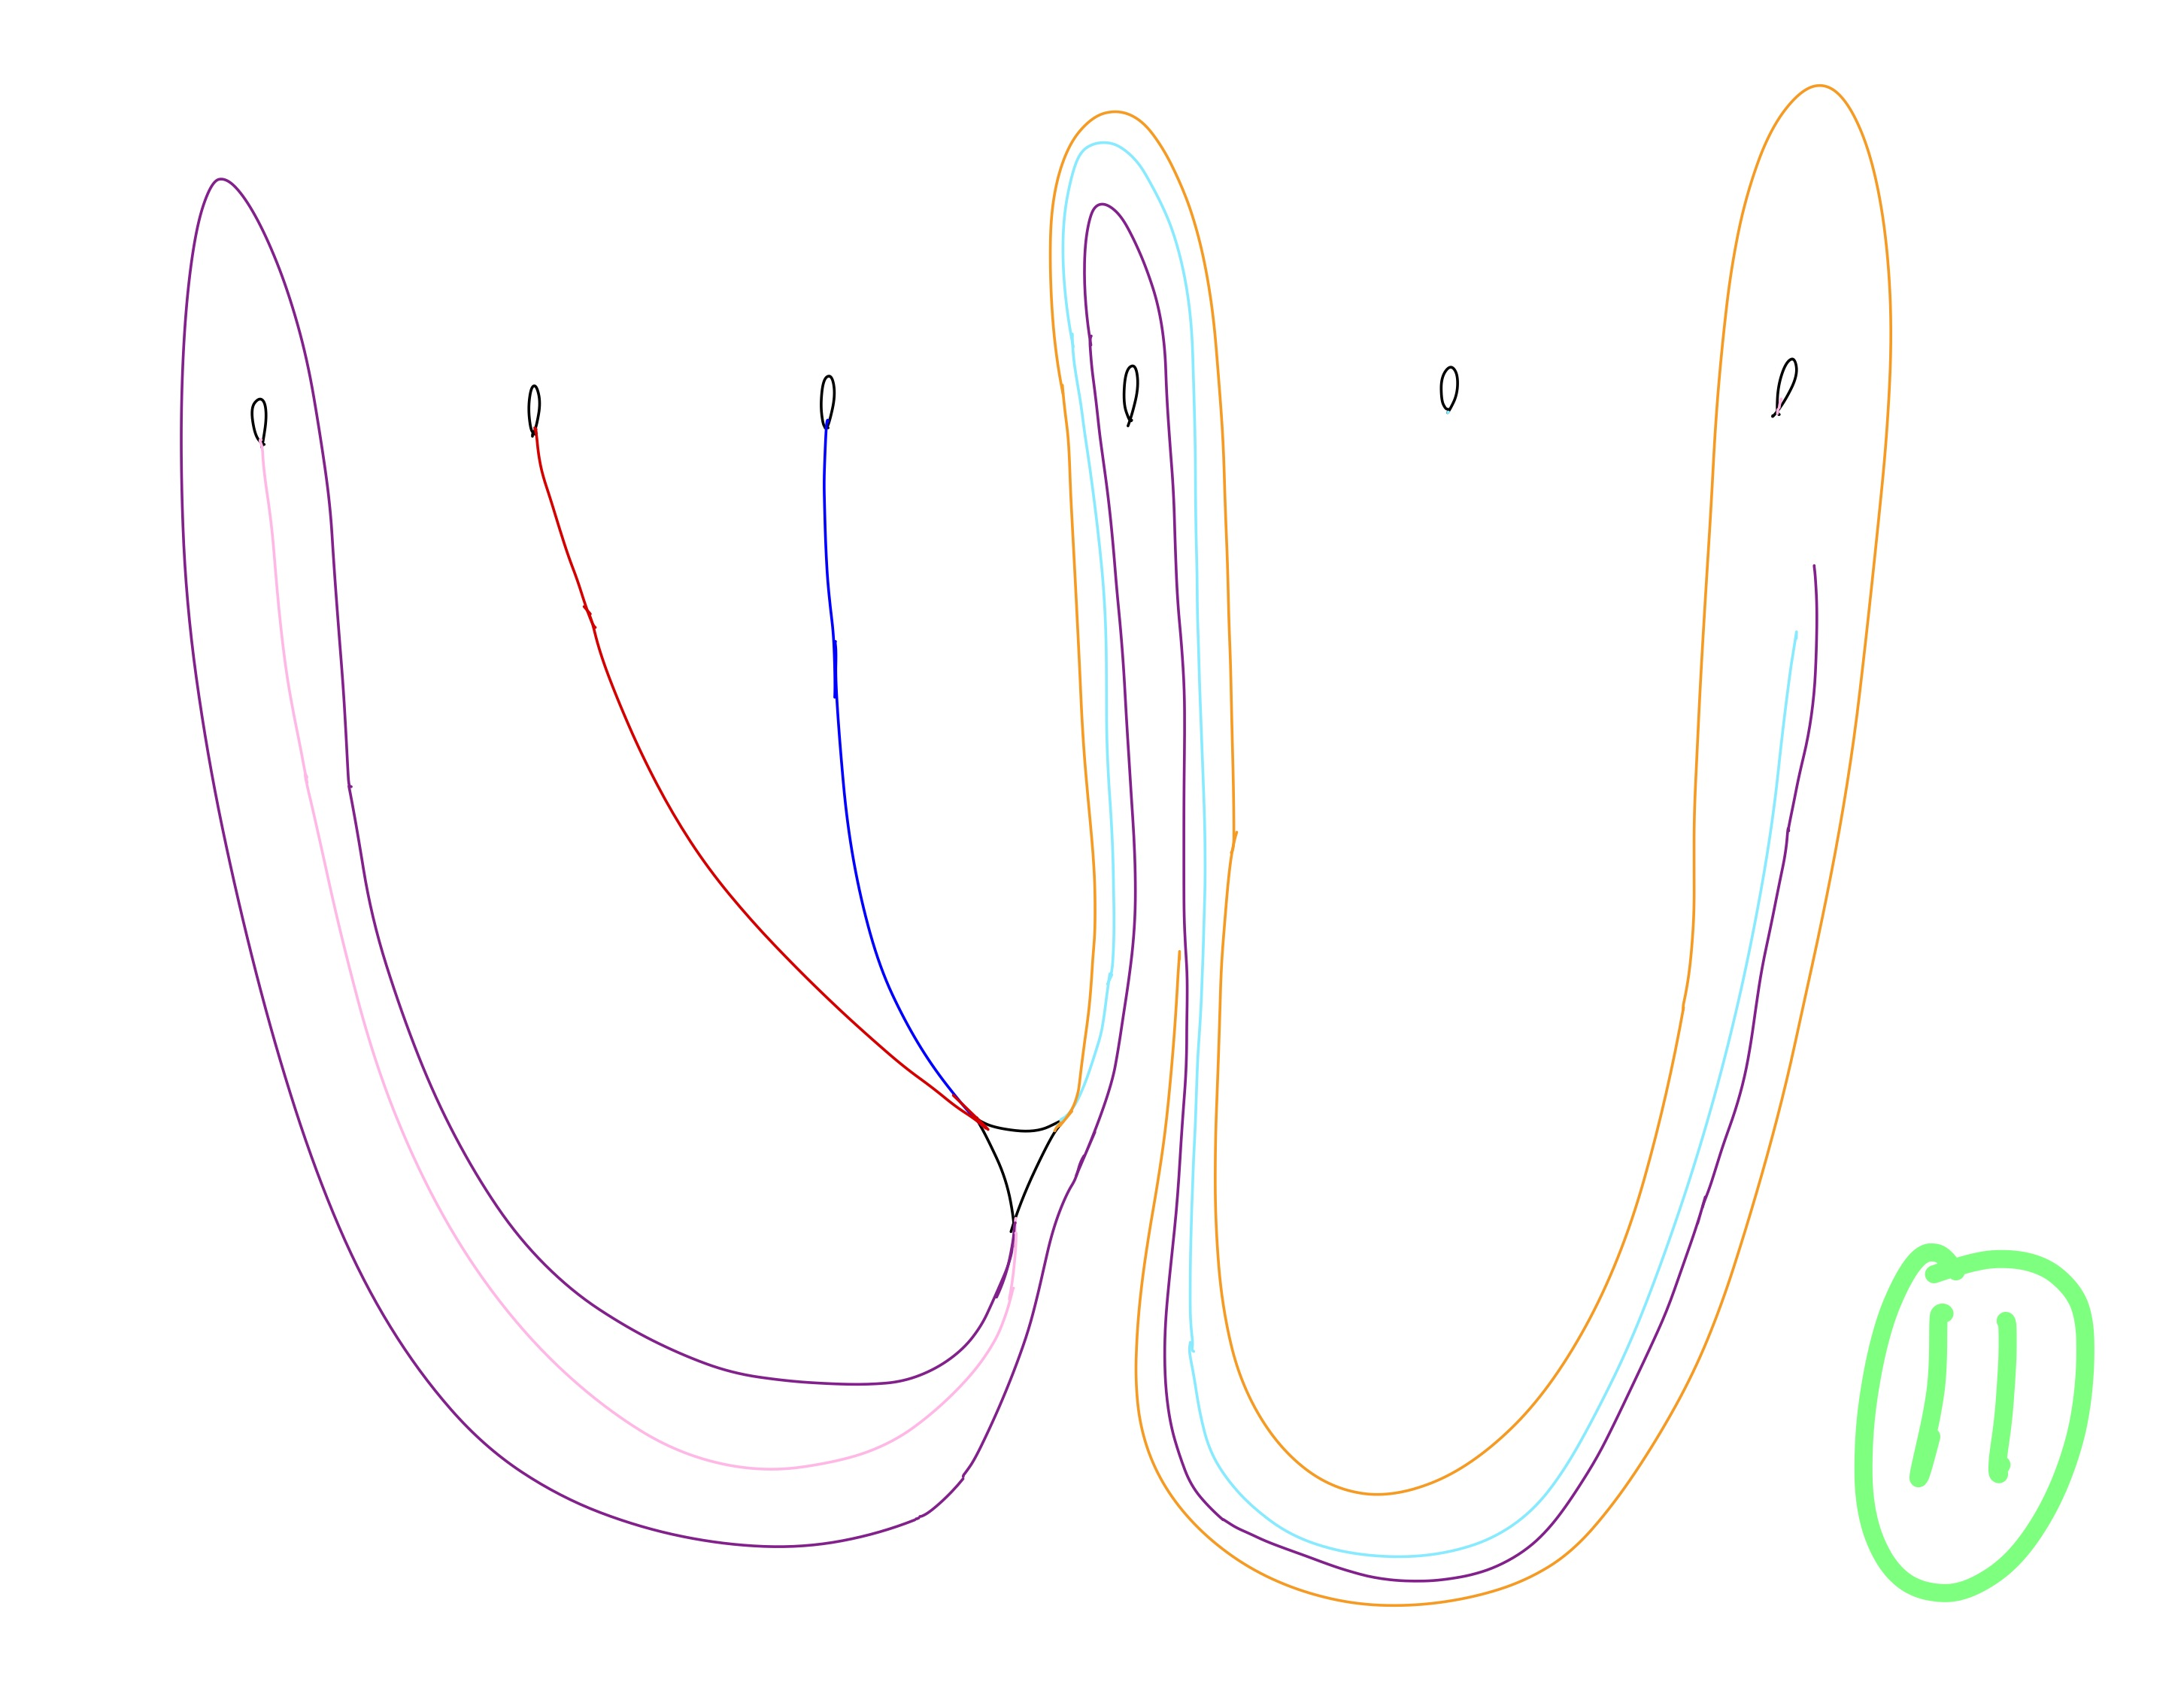
\includegraphics[width=\linewidth, height=0.45\textheight, keepaspectratio]{figures_braid/figures_candelabra/Candelabra Braid 11 Fardel-1.jpg}
    \caption{Train Track Map Candidate Family 11 of the Candelabra.}
    \label{fig:candelabra_braid_b11_map}
\end{figure*}

The inverse of the following braid carries this family of train track maps:
\[
b_{11}^c = \sigma_4 \sigma_5^m \sigma_4^k \sigma_{1} \sigma_{2} \sigma_{3} \sigma_{4} \circ F \circ G
\]
where $G$ is the braid of Section \ref{sec:braid G}, and $k,m\geq 1$ ($k,m\in \mathbb{Z}$) are the twisting parameters. This is shown in Figure \ref{fig:candelabra_braid_b11}.

\begin{figure*}[p]
    \centering
    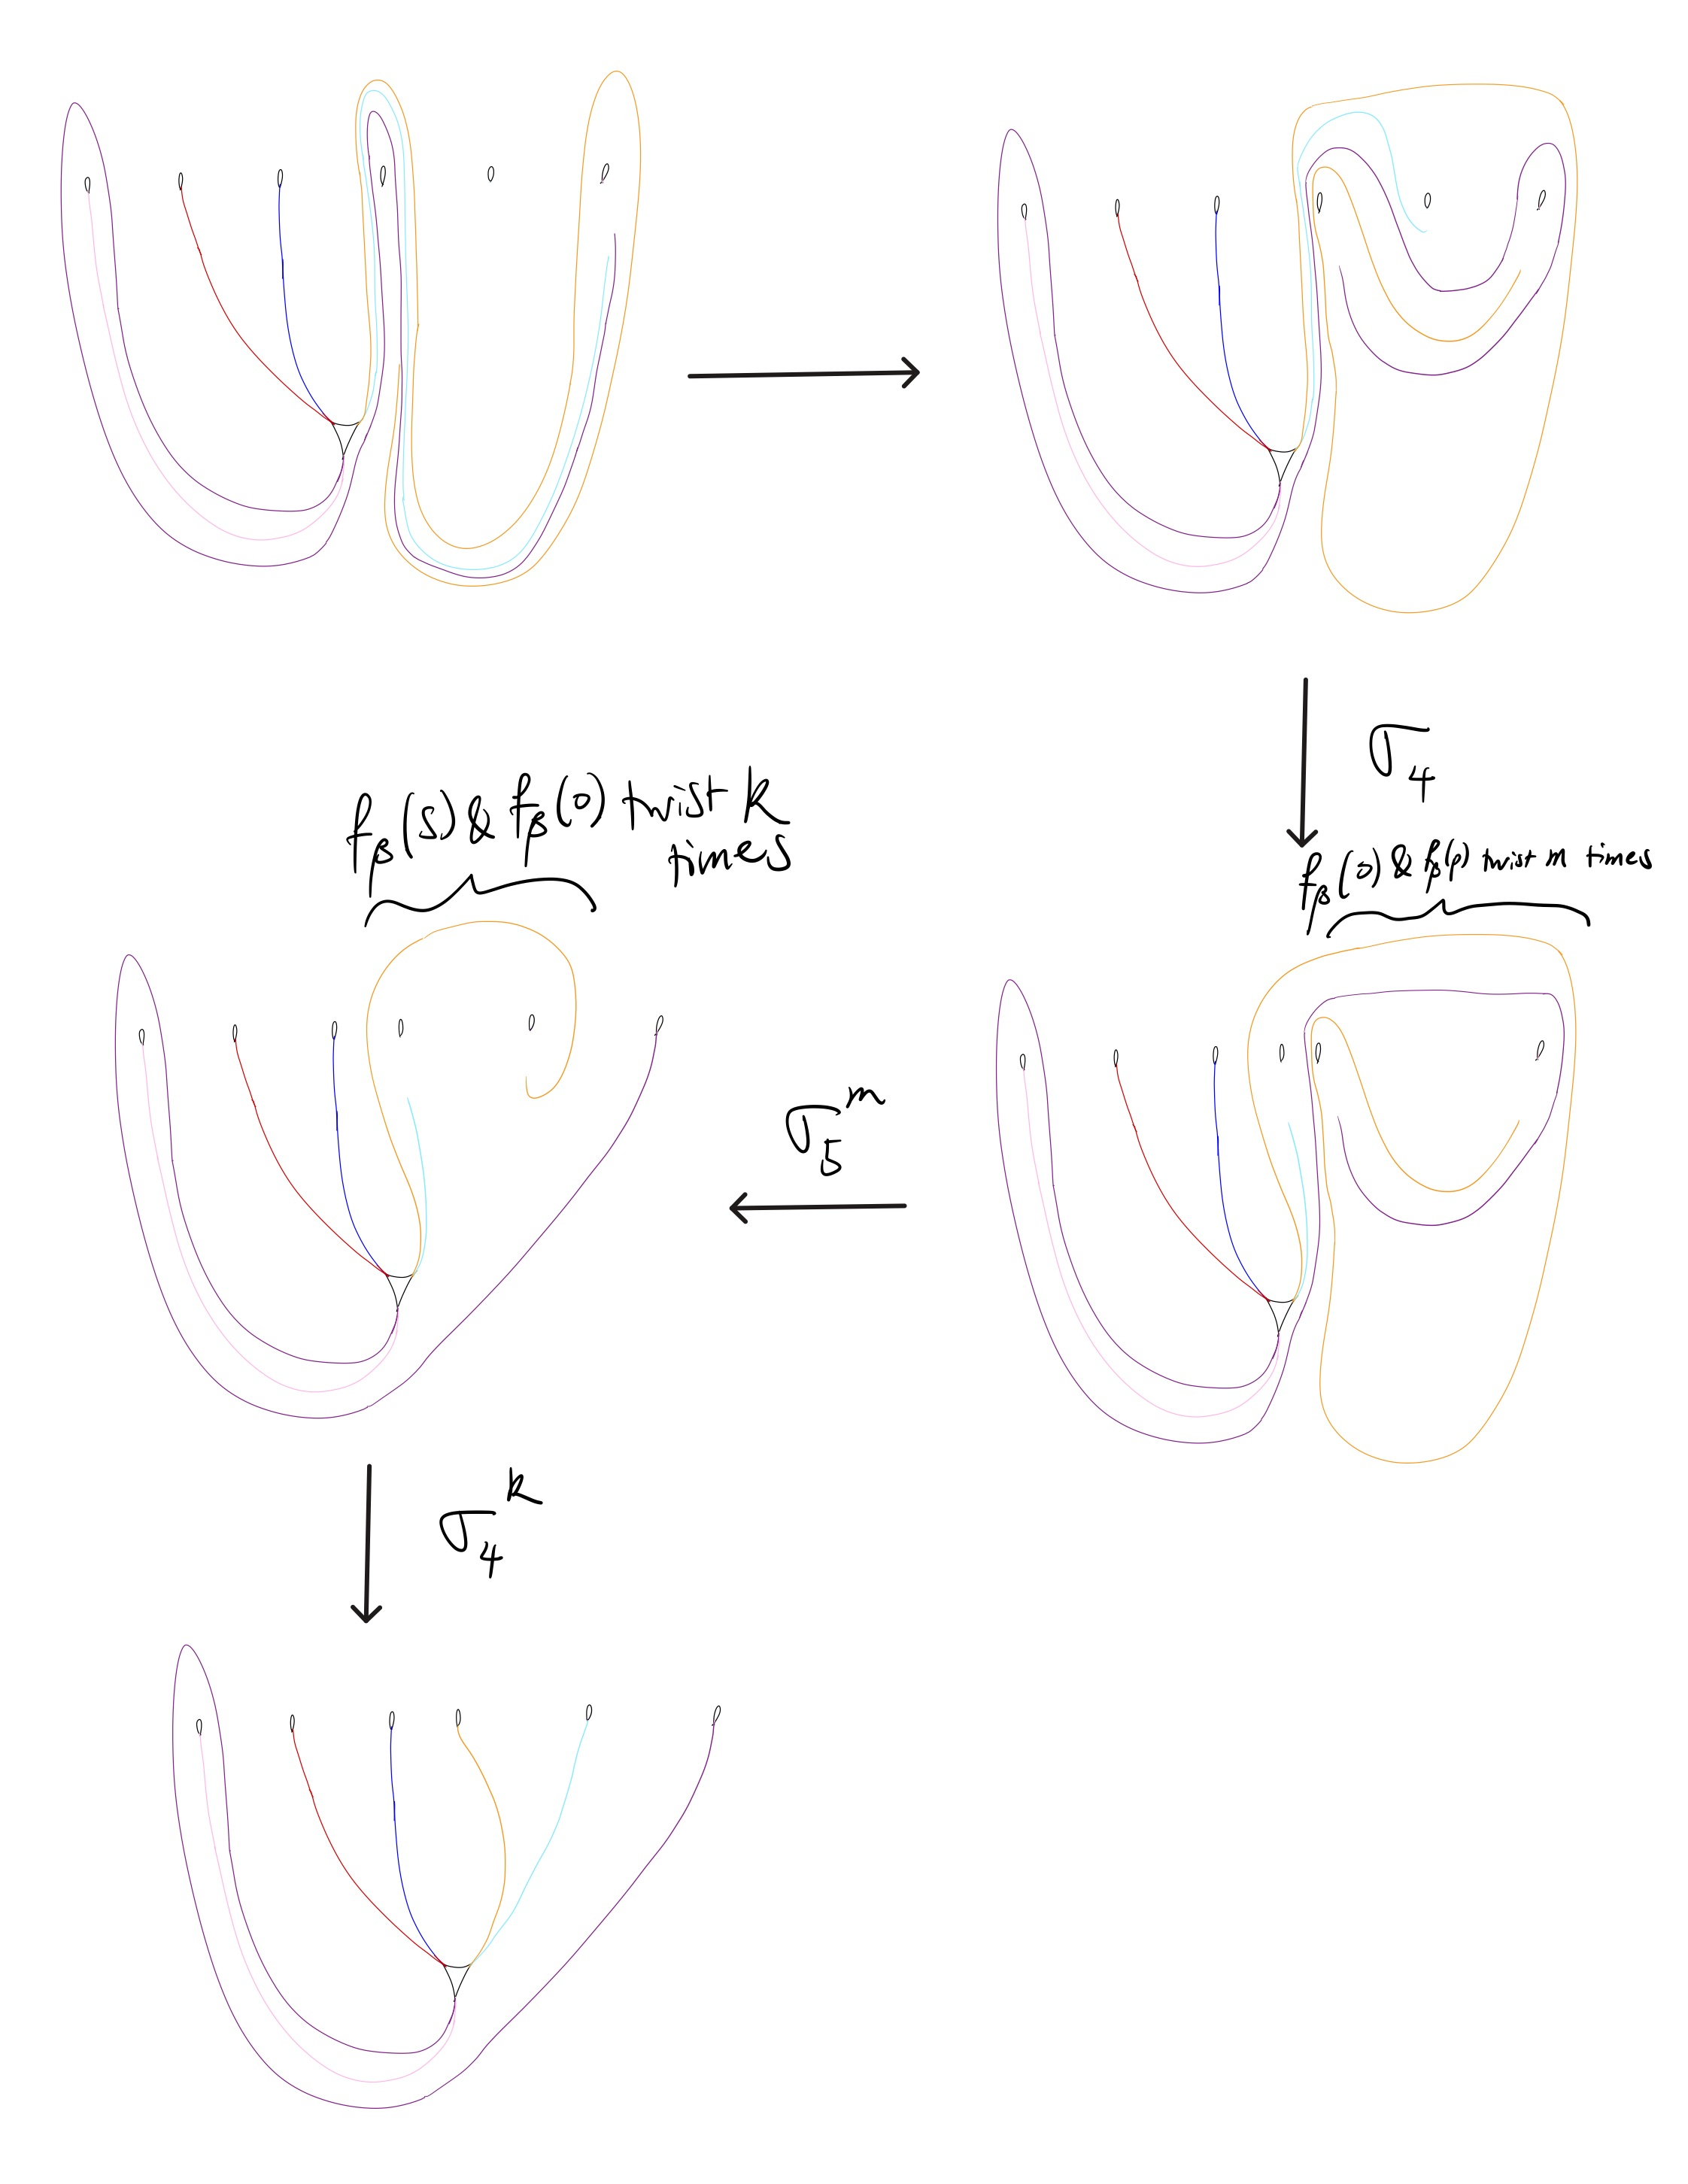
\includegraphics[width=\linewidth, height=0.45\textheight, keepaspectratio]{figures_braid/figures_candelabra/Candelabra Braid 11 Fardel-2.jpg}\\
    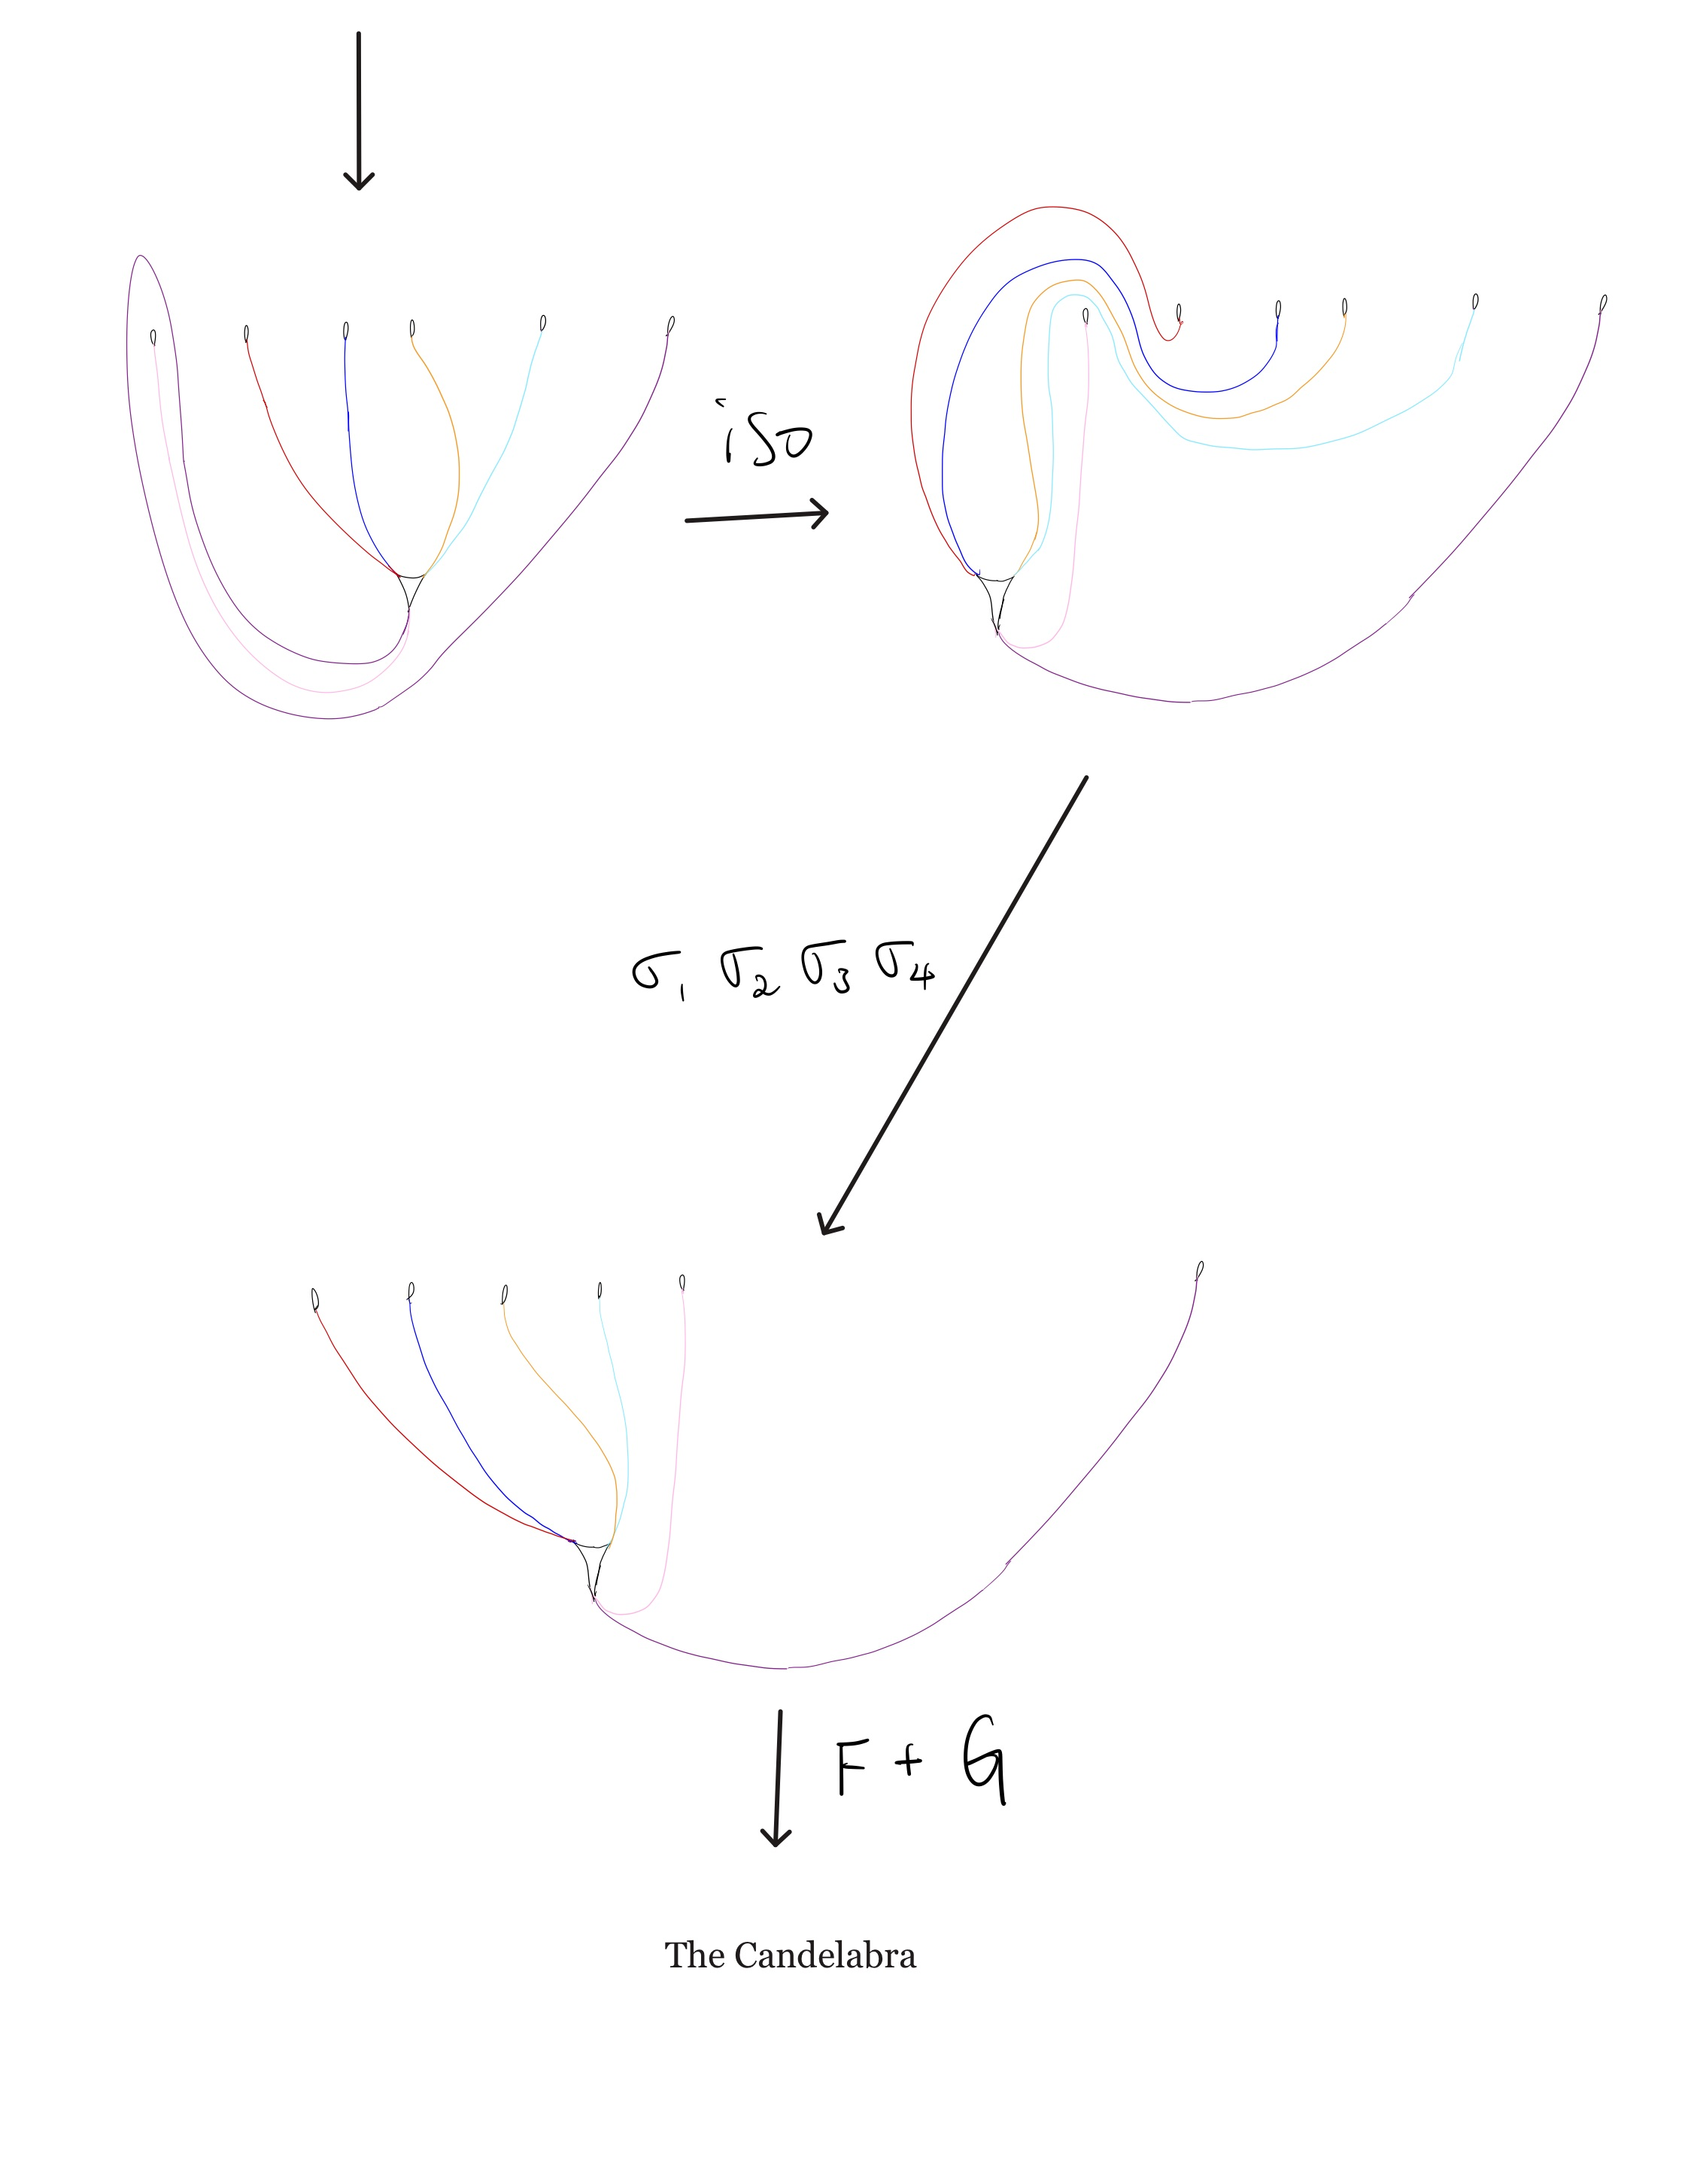
\includegraphics[width=\linewidth, height=0.45\textheight, keepaspectratio]{figures_braid/figures_candelabra/Candelabra Braid 11 Fardel-3.jpg}   
    \caption{This sequence shows the inverse of the braid $b_{11}^c$ carries Train Track Candidate Family 11.}
    \label{fig:candelabra_braid_b11}
\end{figure*}

\clearpage
\section{Candidate Family 12}
Train Track Map Candidate Family 12 of the Candelabra train track is shown in Figure \ref{fig:candelabra_braid_b12_map}. Note there is twisting between $\fbo$ and $\fbs$. See \ref{Tantivy} for details.

\begin{figure*}[ht]
    \centering
    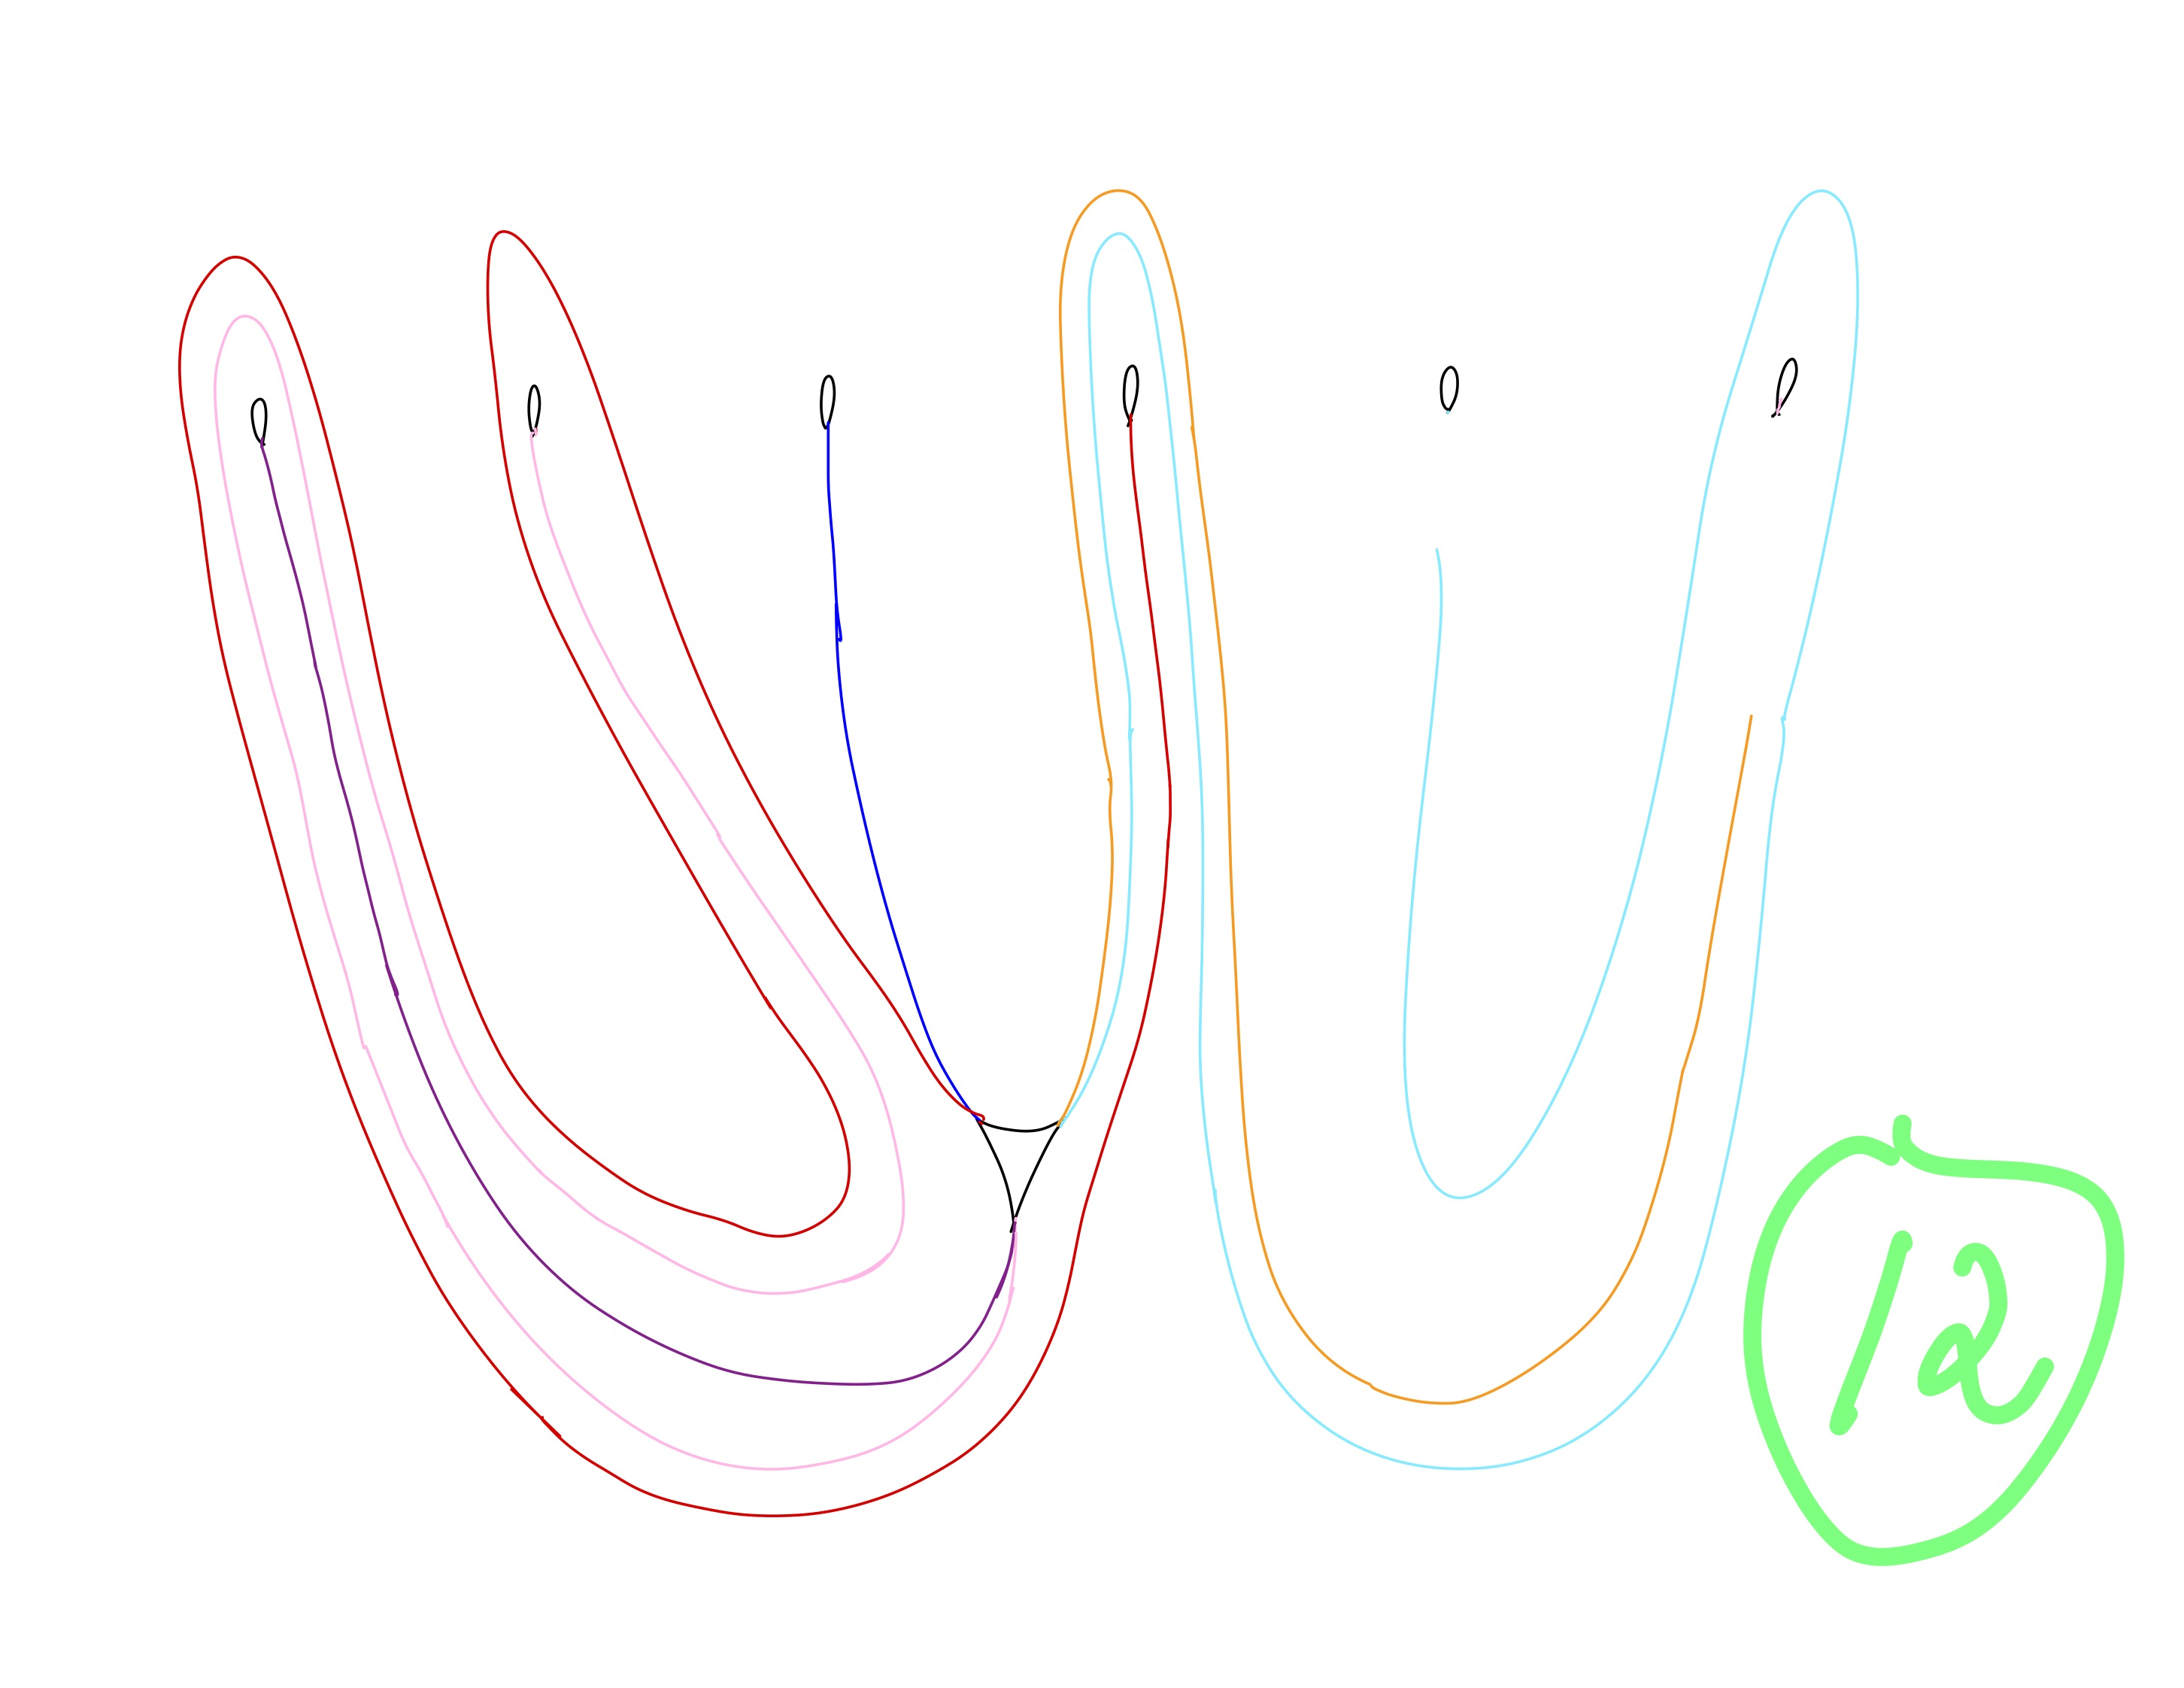
\includegraphics[width=\linewidth, height=0.45\textheight, keepaspectratio]{figures_braid/figures_candelabra/Candelabra Braid 12 Tantivy-1.jpg}
    \caption{Train Track Map Candidate Family 12 of the Candelabra.}
    \label{fig:candelabra_braid_b12_map}
\end{figure*}

The inverse of the following braid carries this family of train track maps:
\[
b_{12}^c = (\sigma_{5}^{-1})^k \sigma_{4} \sigma_{5} \sigma_{1} \sigma_{2} \sigma_{1} \sigma_{3} \sigma_{2} \sigma_{4} \sigma_{3} \sigma_{4} \sigma_{4}
\]
where $k\geq 1$ ($k\in \mathbb{Z}$) is the twisting parameter. This is shown in Figure \ref{fig:candelabra_braid_b12}.

\begin{figure*}[p]
    \centering
    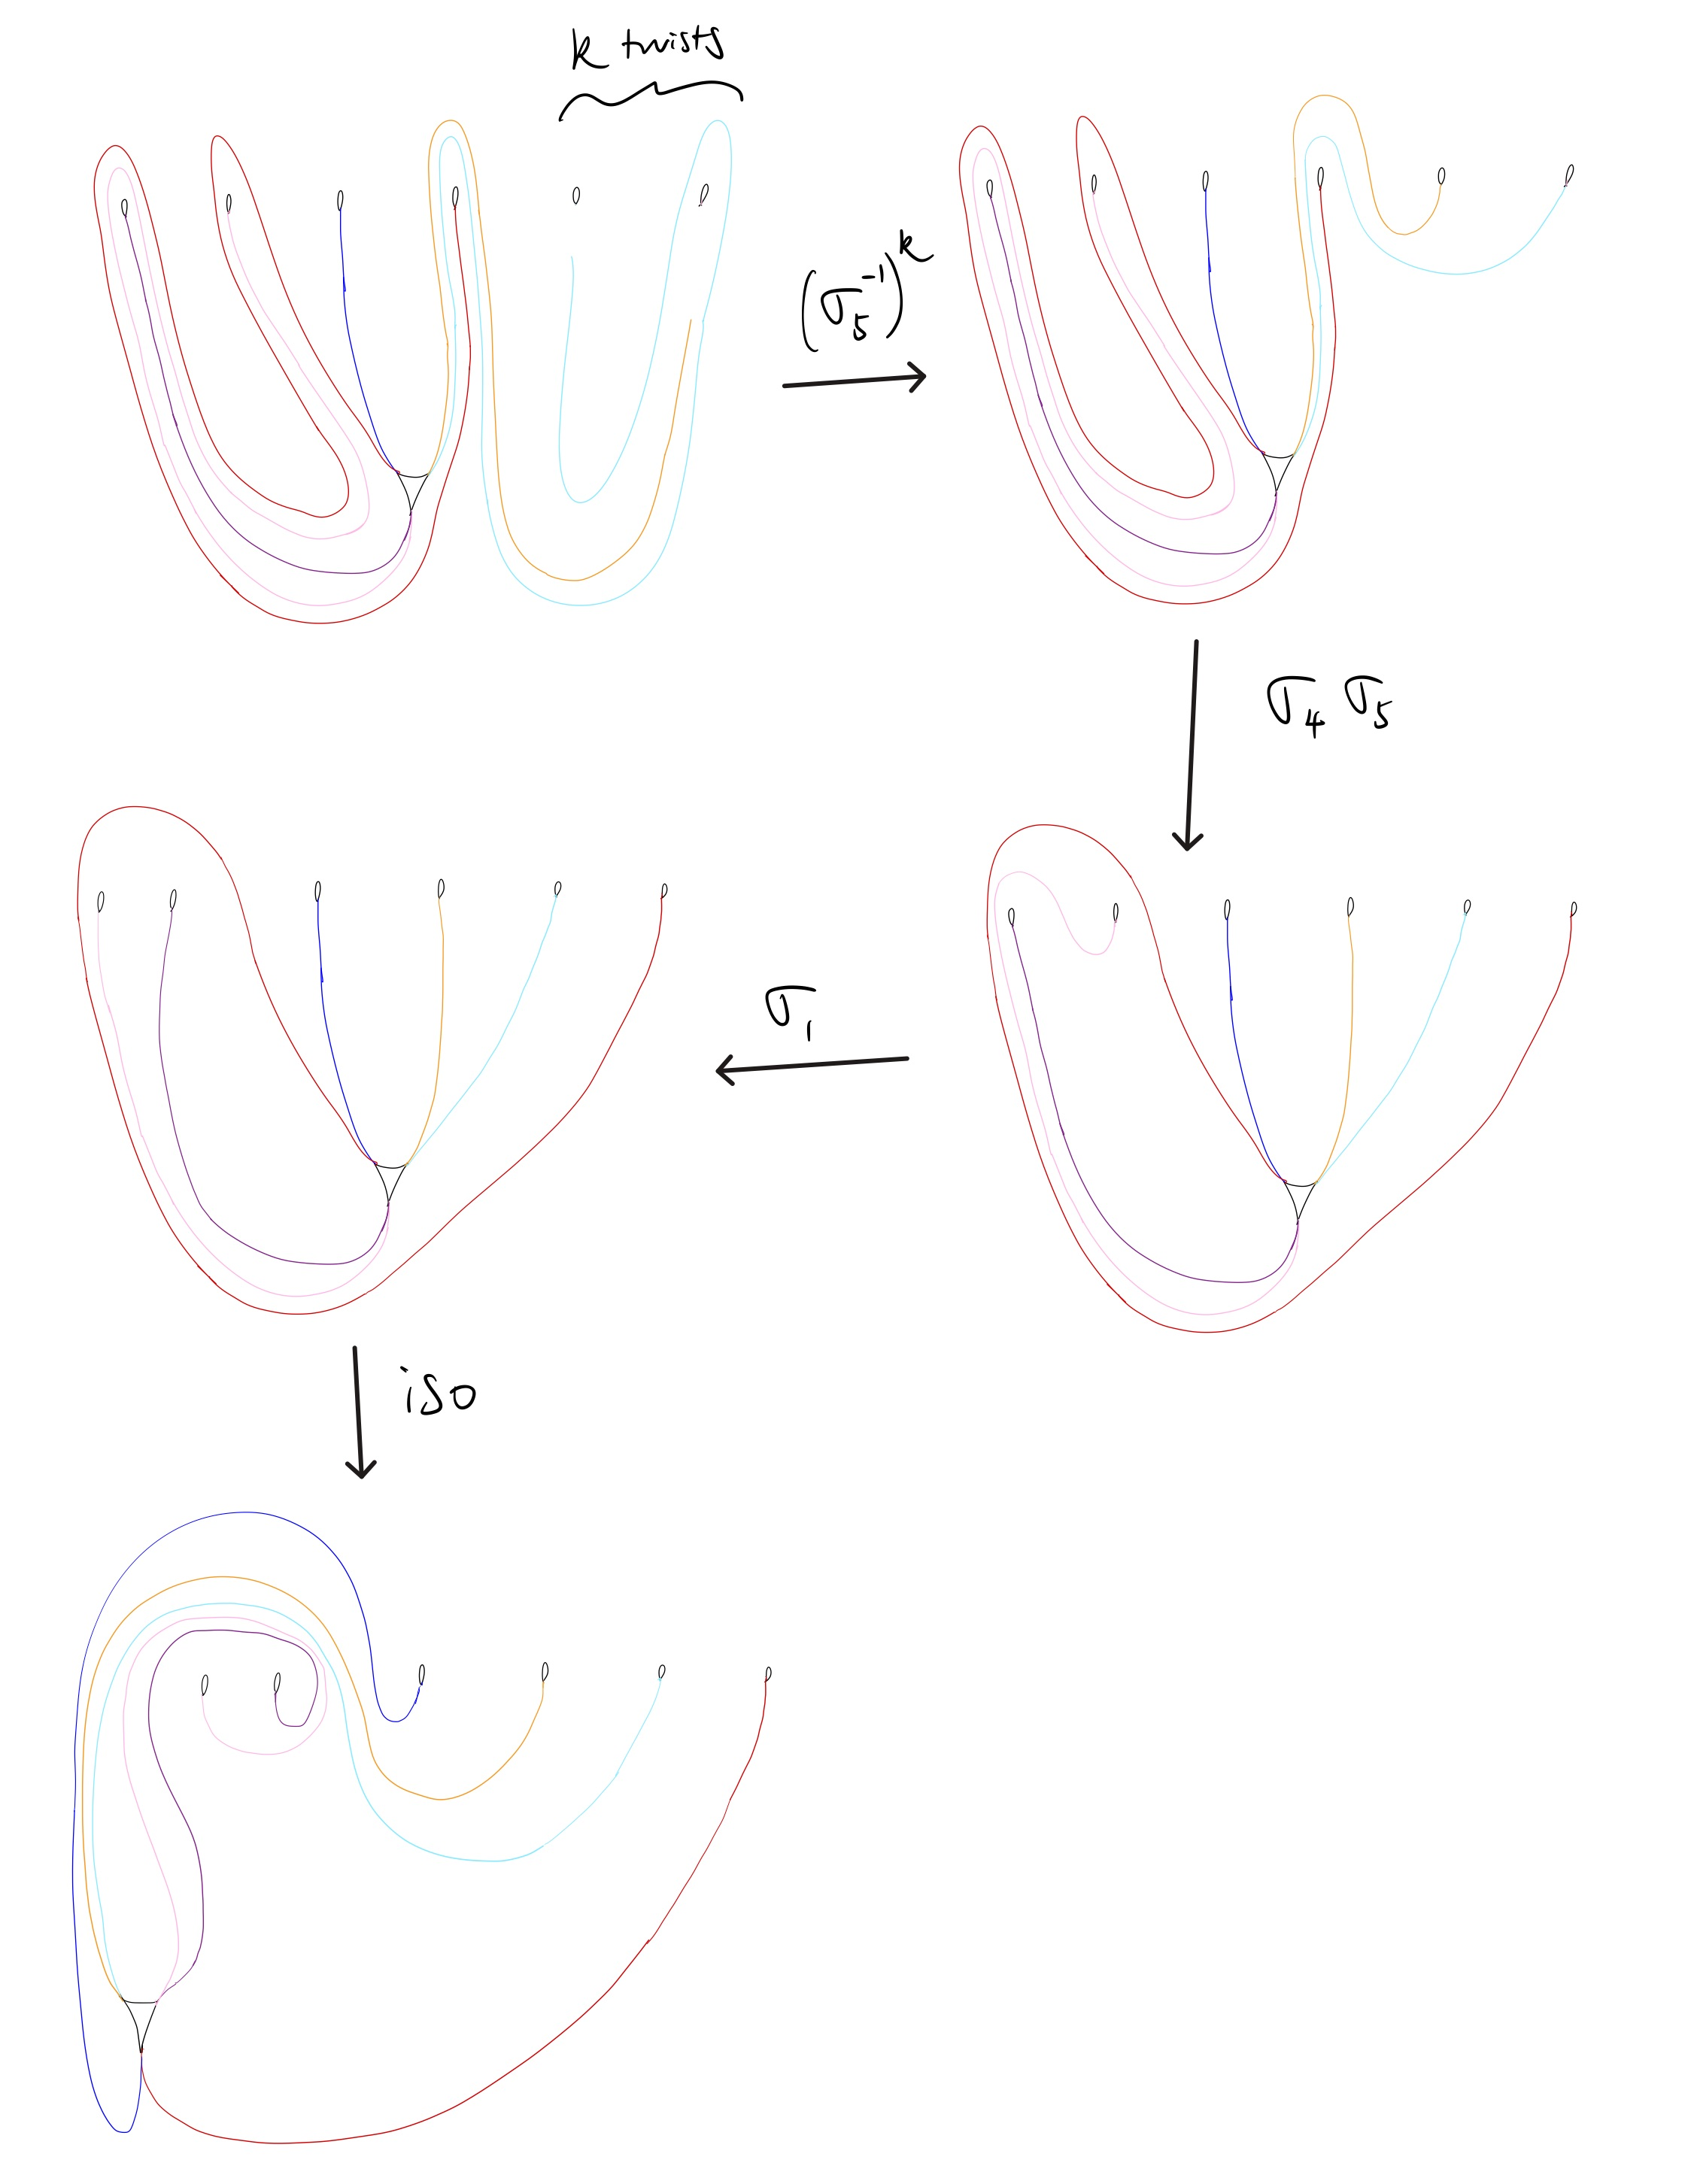
\includegraphics[width=\linewidth, height=0.45\textheight, keepaspectratio]{figures_braid/figures_candelabra/Candelabra Braid 12 Tantivy-2.jpg}\\
    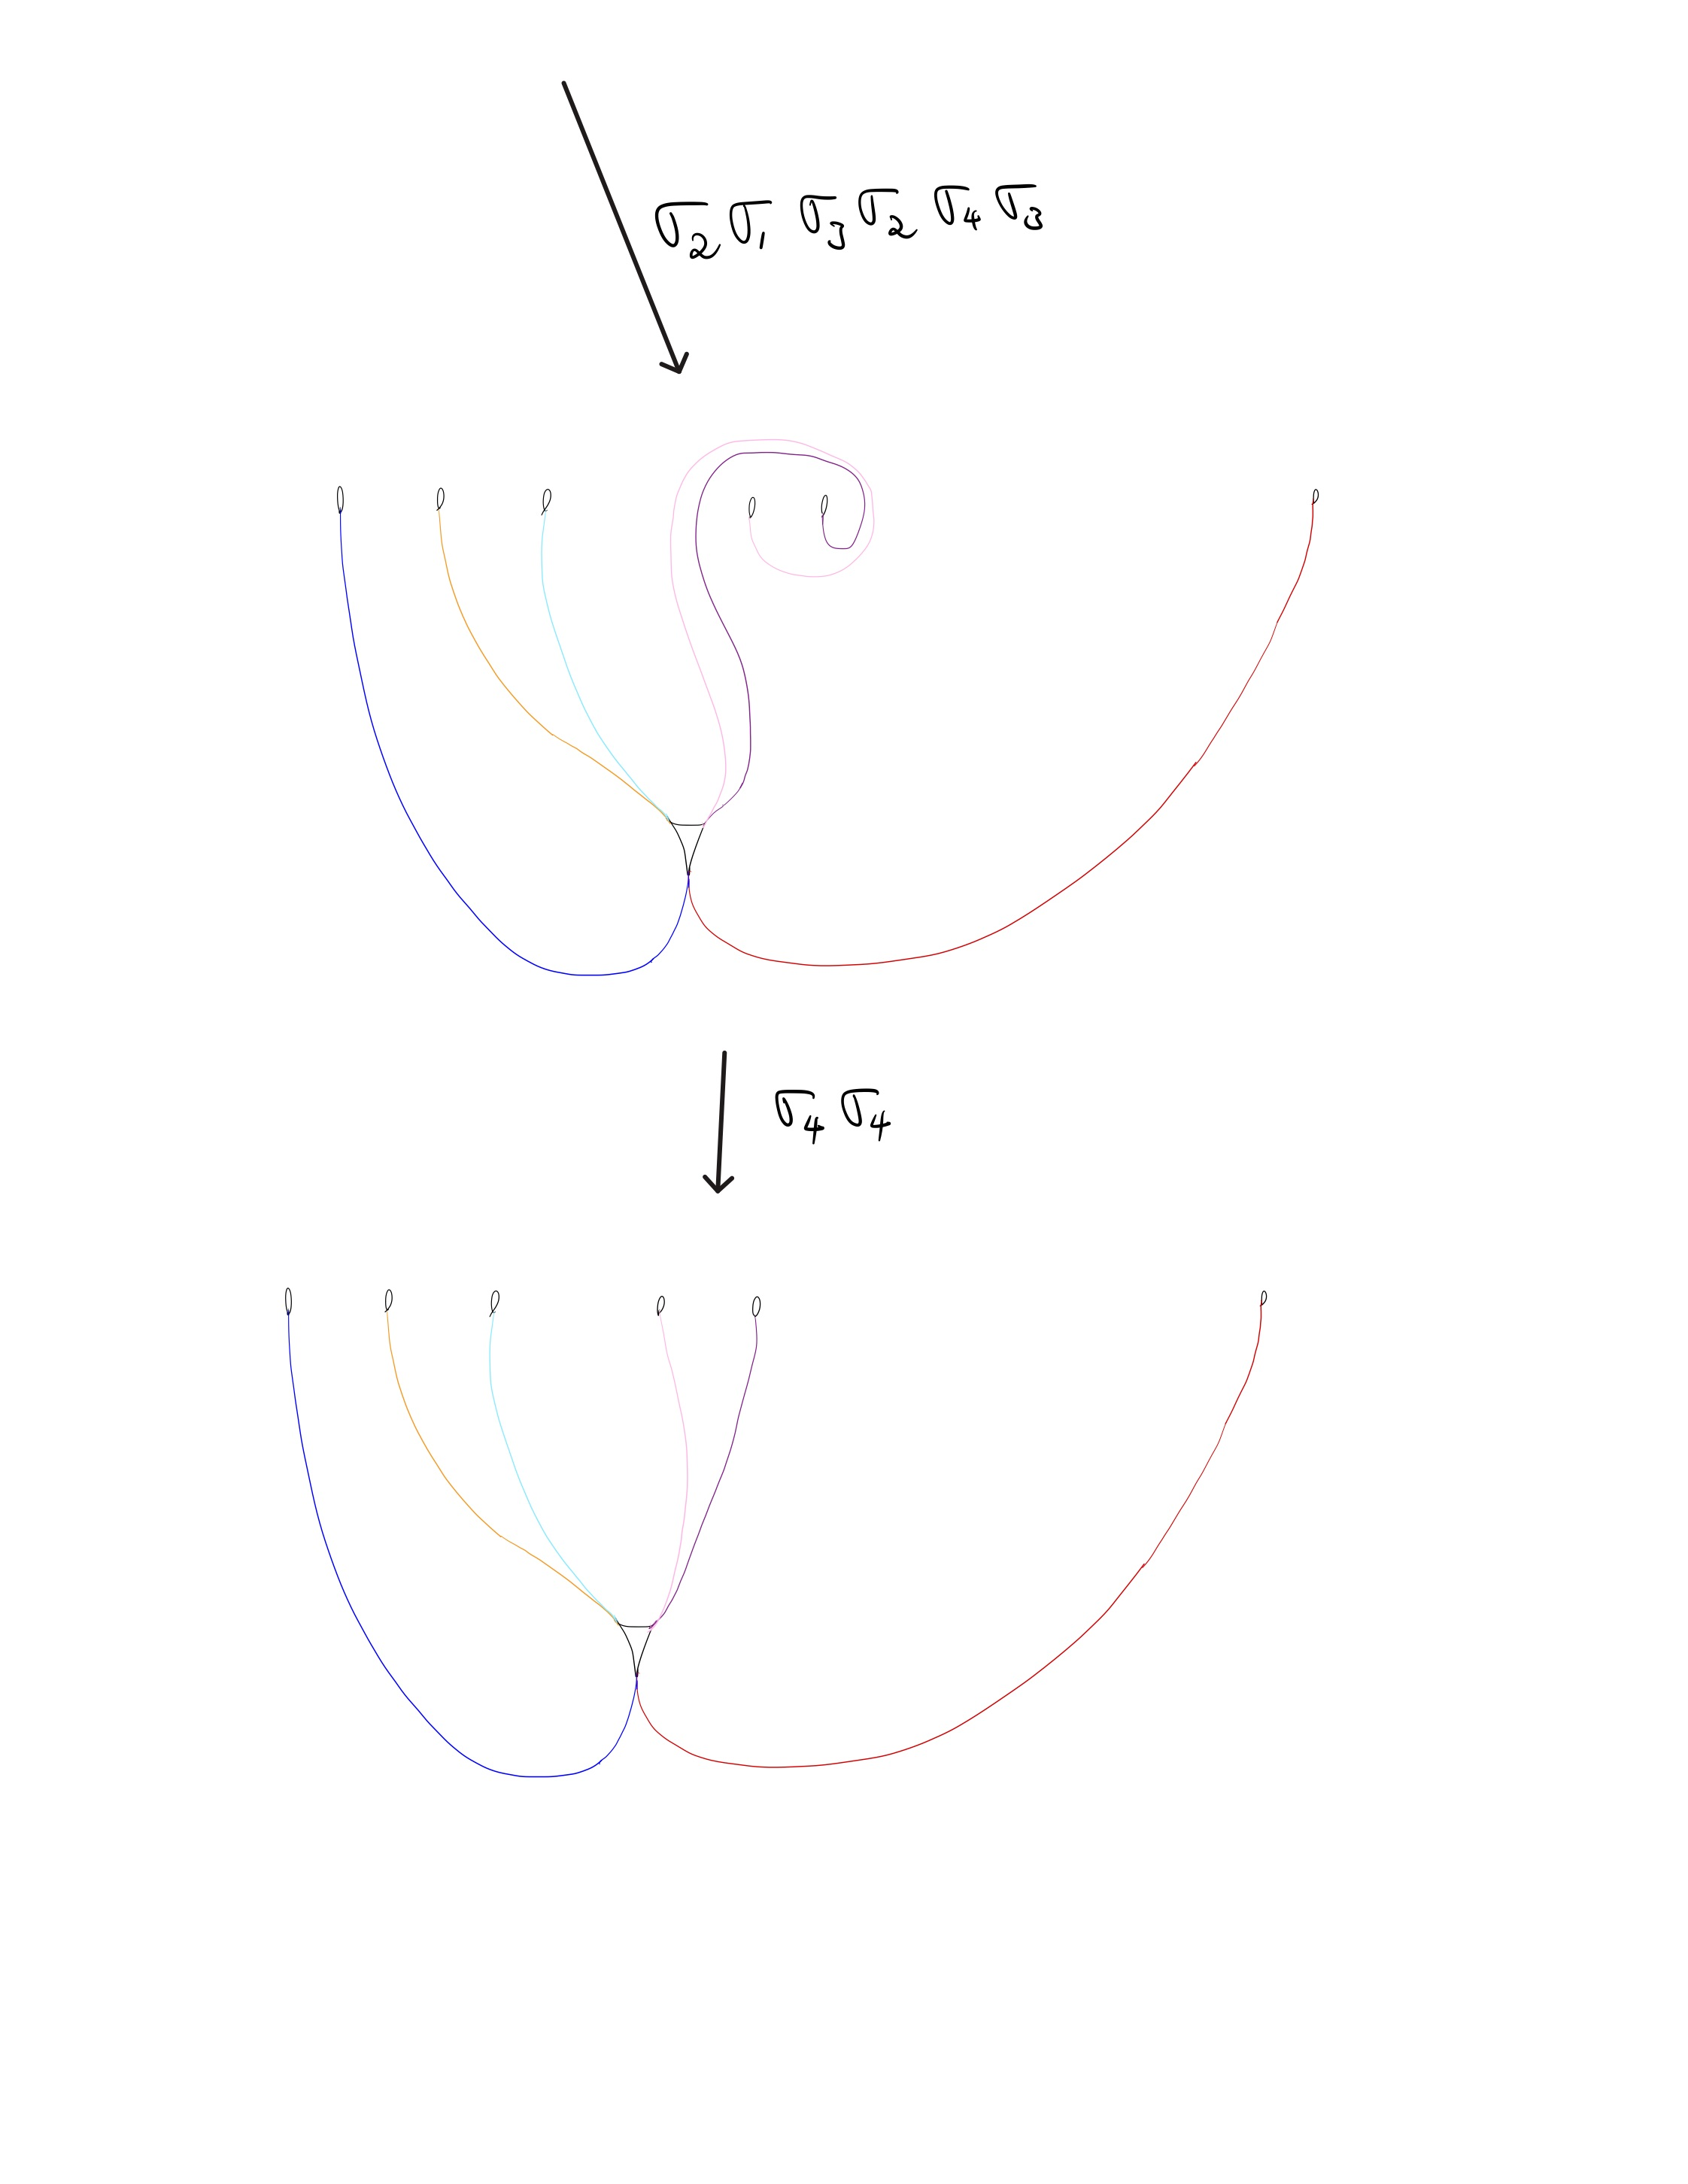
\includegraphics[width=\linewidth, height=0.45\textheight, keepaspectratio]{figures_braid/figures_candelabra/Candelabra Braid 12 Tantivy-3.jpg}   
    \caption{This sequence shows the inverse of the braid $b_{12}^c$ carries Train Track Candidate Family 12.}
    \label{fig:candelabra_braid_b12}
\end{figure*}

\clearpage

\section{Candidate 13}
Train Track Map Candidate 13 of the Candelabra train track is shown in Figure \ref{fig:candelabra_braid_b13_map}.

\begin{figure*}[ht]
    \centering
    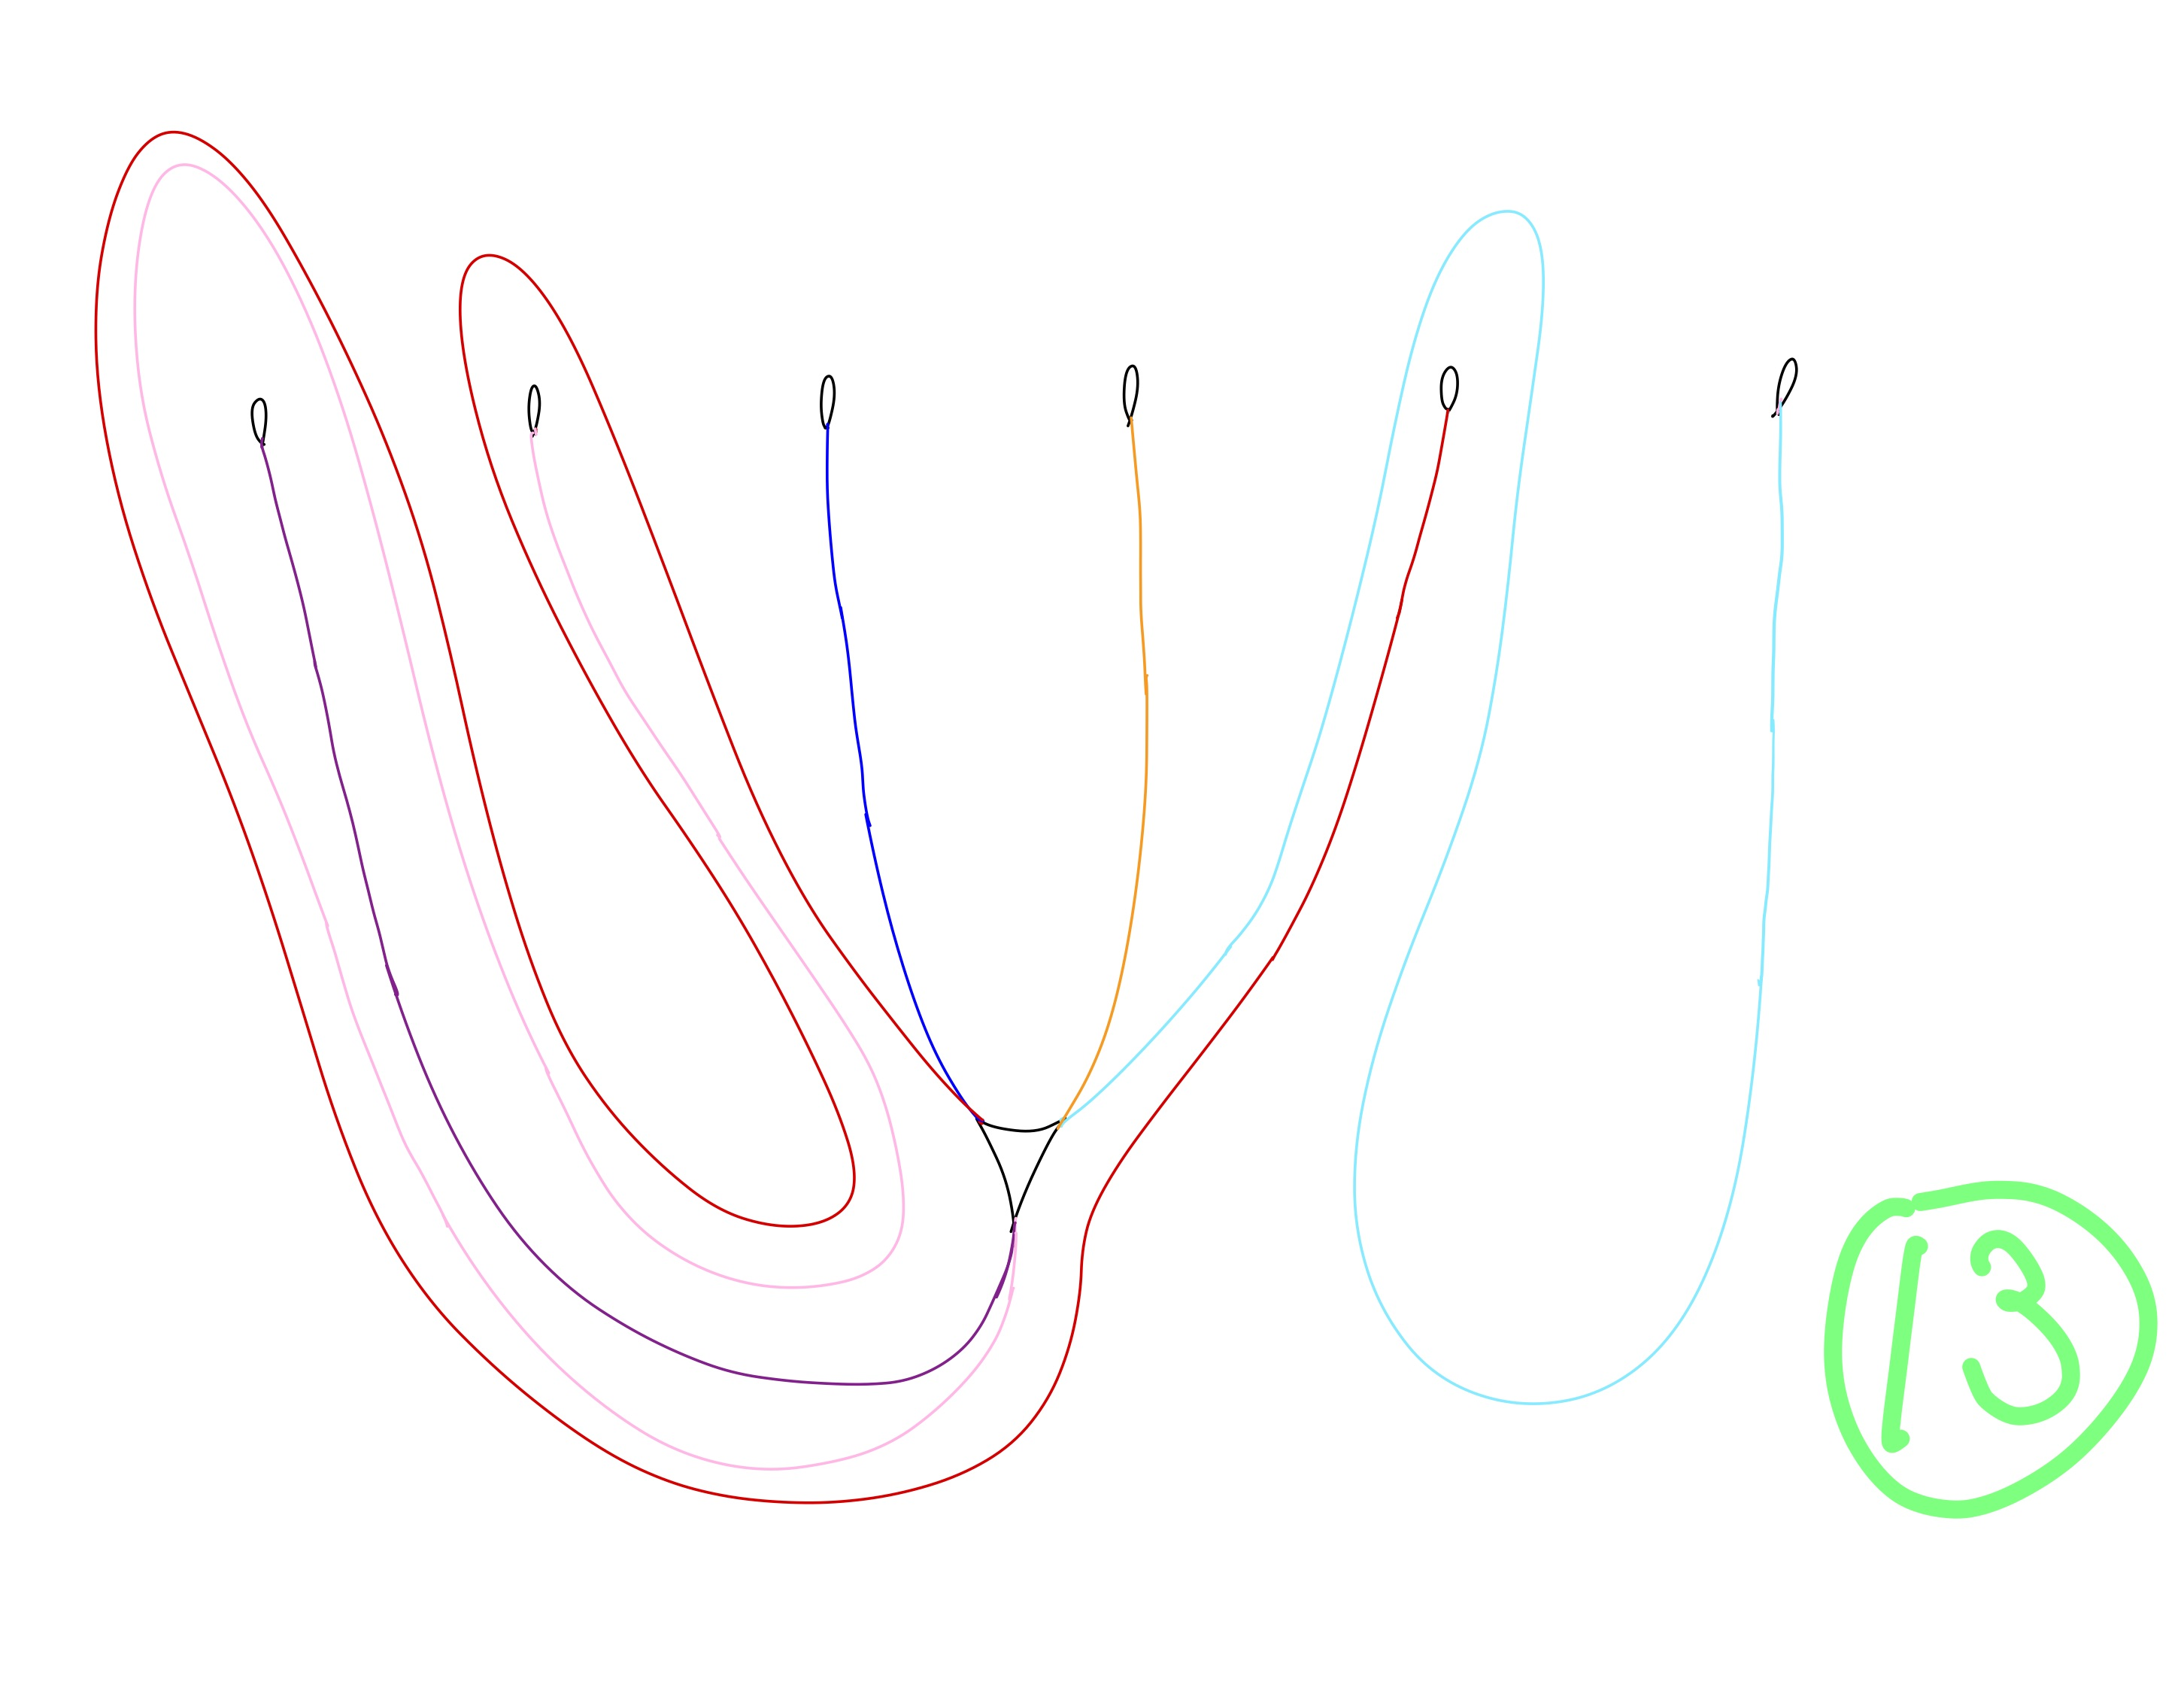
\includegraphics[width=\linewidth, height=0.45\textheight, keepaspectratio]{figures_braid/figures_candelabra/Candelabra Braid 13 Tantivy-1.jpg}
    \caption{Train Track Map Candidate 13 of the Candelabra.}
    \label{fig:candelabra_braid_b13_map}
\end{figure*}

The inverse of the following braid carries this train track map:
\[
b_{13}^c = \sigma_{5} \sigma_{1} \sigma_{2} \sigma_{1} \sigma_{3} \sigma_{2} \sigma_{4} \sigma_{3} \sigma_{4} \sigma_{4}
\]

This is shown in Figure \ref{fig:candelabra_braid_b13}.

\begin{figure*}[p]
    \centering
    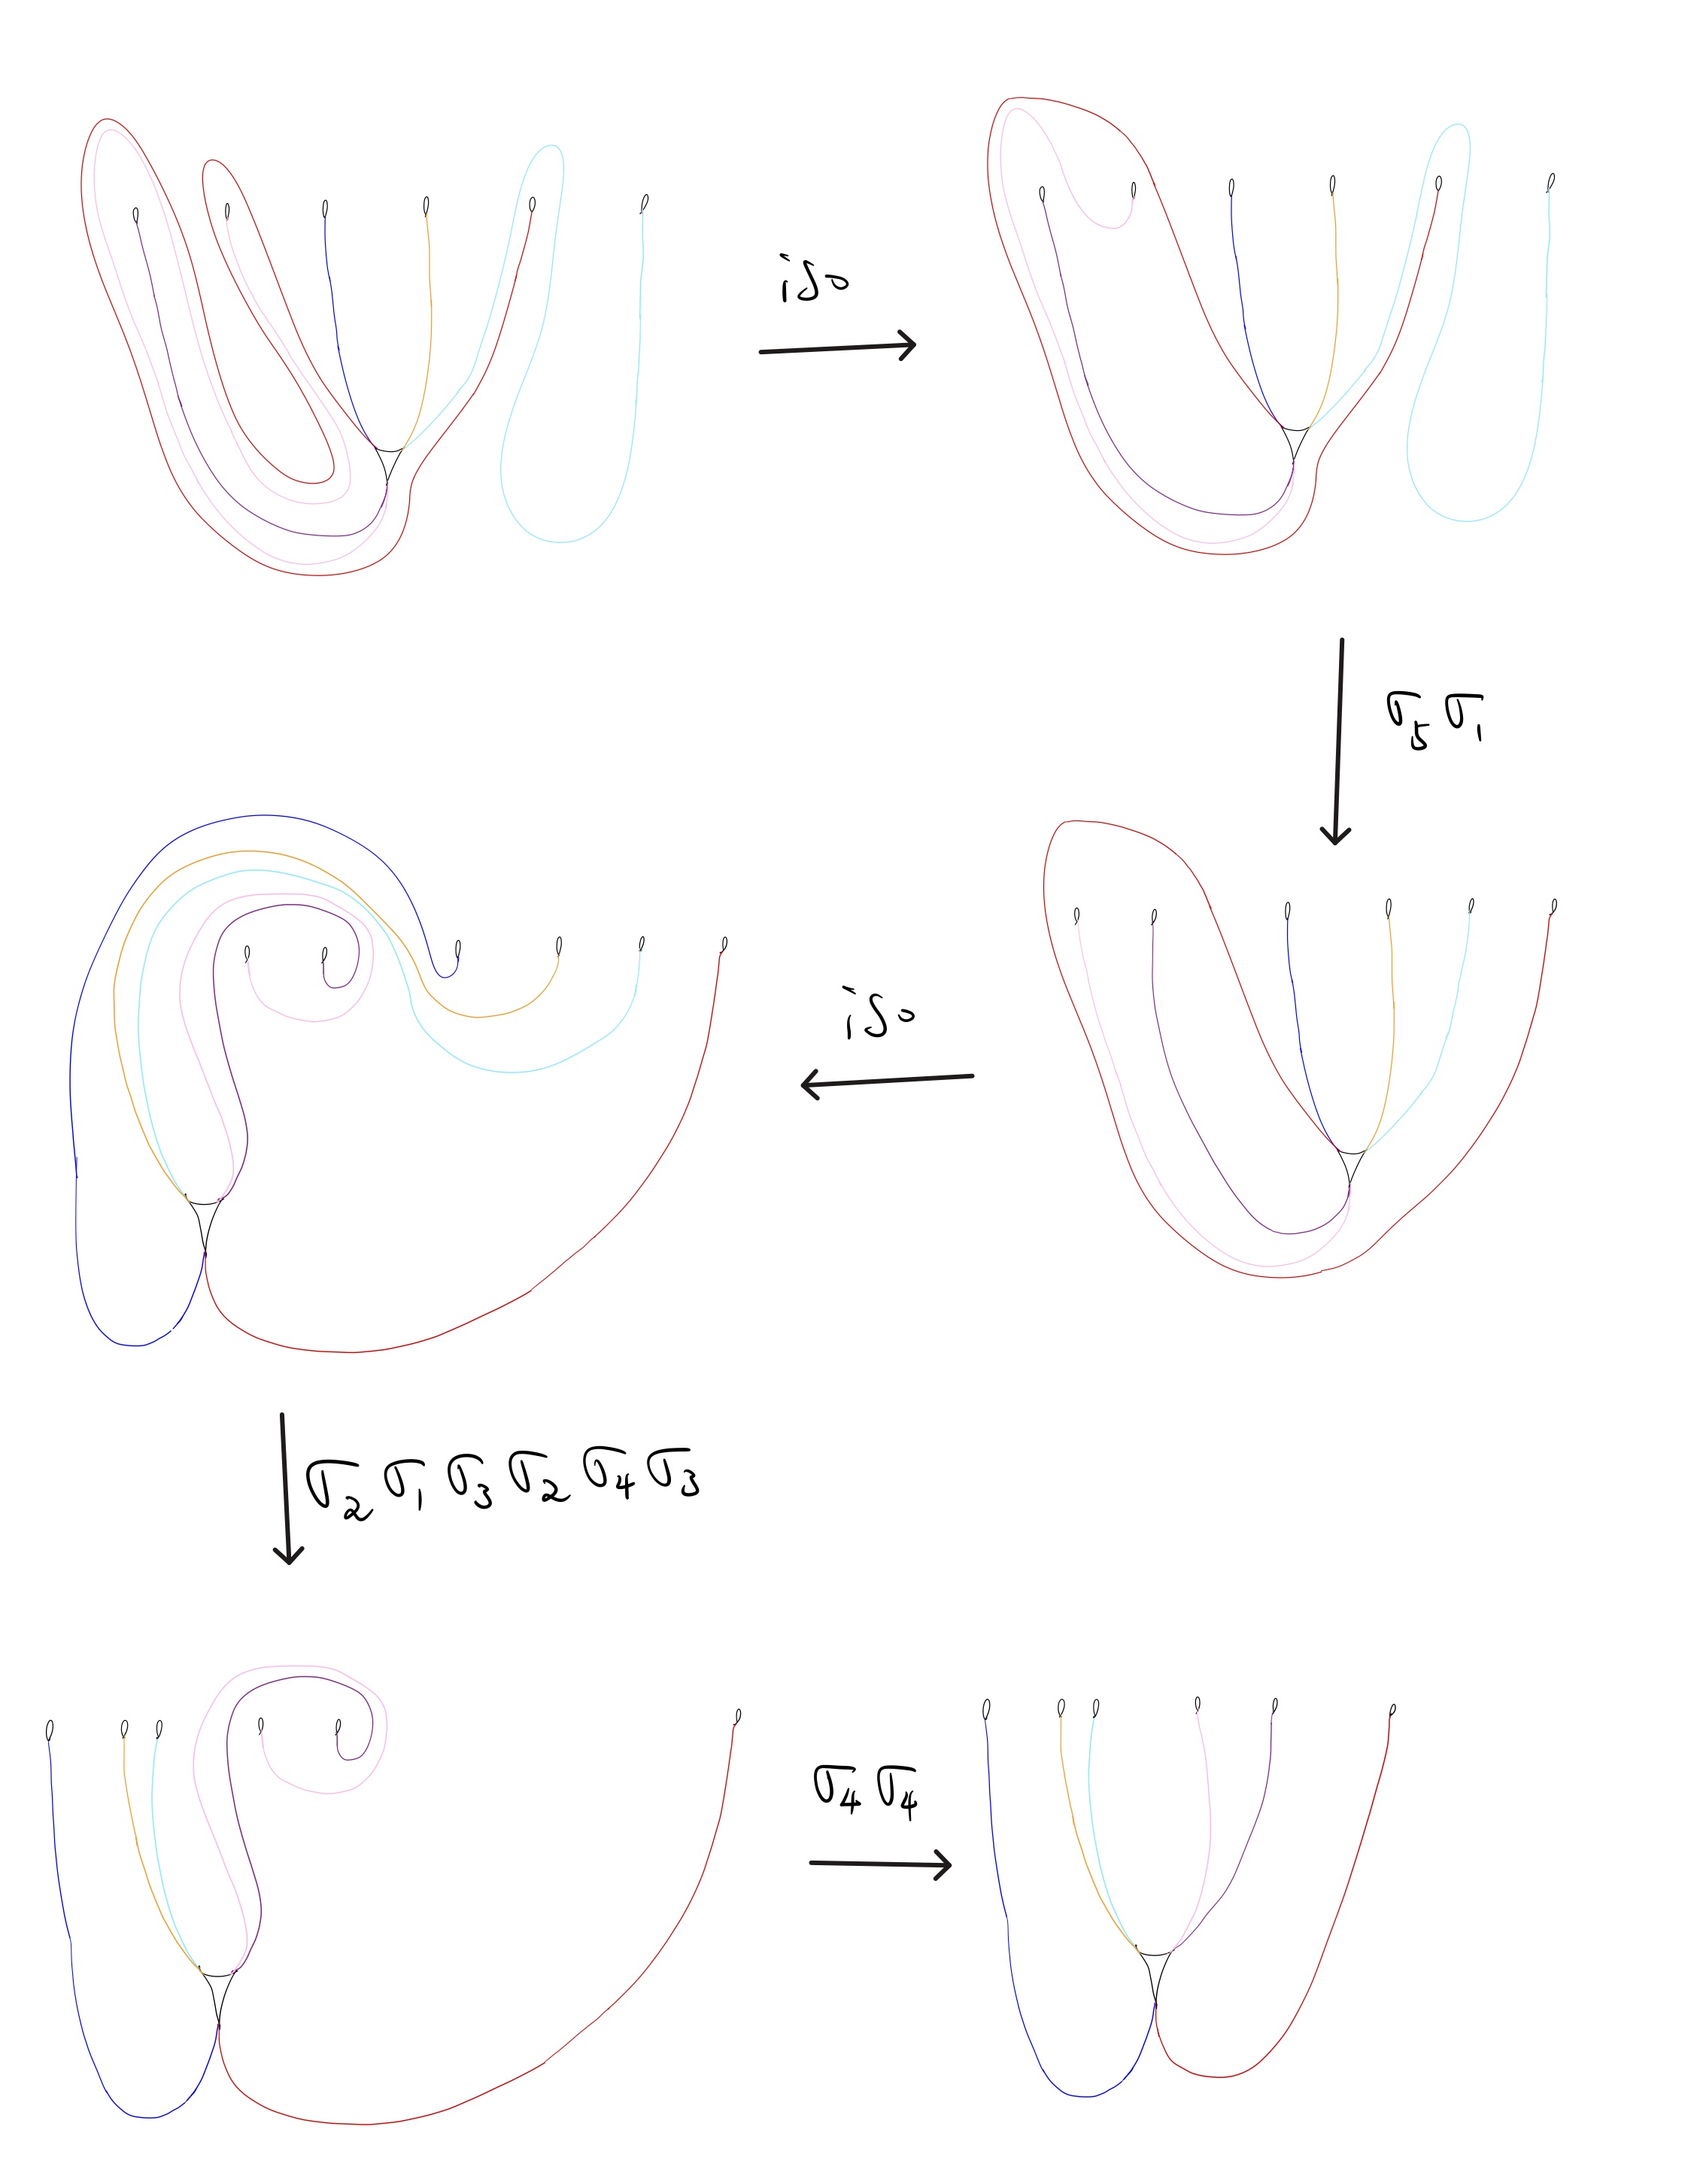
\includegraphics[width=\linewidth, height=0.45\textheight, keepaspectratio]{figures_braid/figures_candelabra/Candelabra Braid 13 Tantivy-2.jpg} 
    \caption{This sequence shows the inverse of the braid $b_{13}^c$ carries Train Track Map Candidate 13.}
    \label{fig:candelabra_braid_b13}
\end{figure*}

\clearpage

\section{Candidate Family 14}
Train Track Map Candidate Family 14 of the Candelabra train track is shown in Figure \ref{fig:candelabra_braid_b14_map}. Note there is twisting between $\fbo$ and $\fbs$; and twisting between $\fbr$ and $\fbb$. See \ref{Tantivy} for details.

\begin{figure*}[ht]
    \centering
    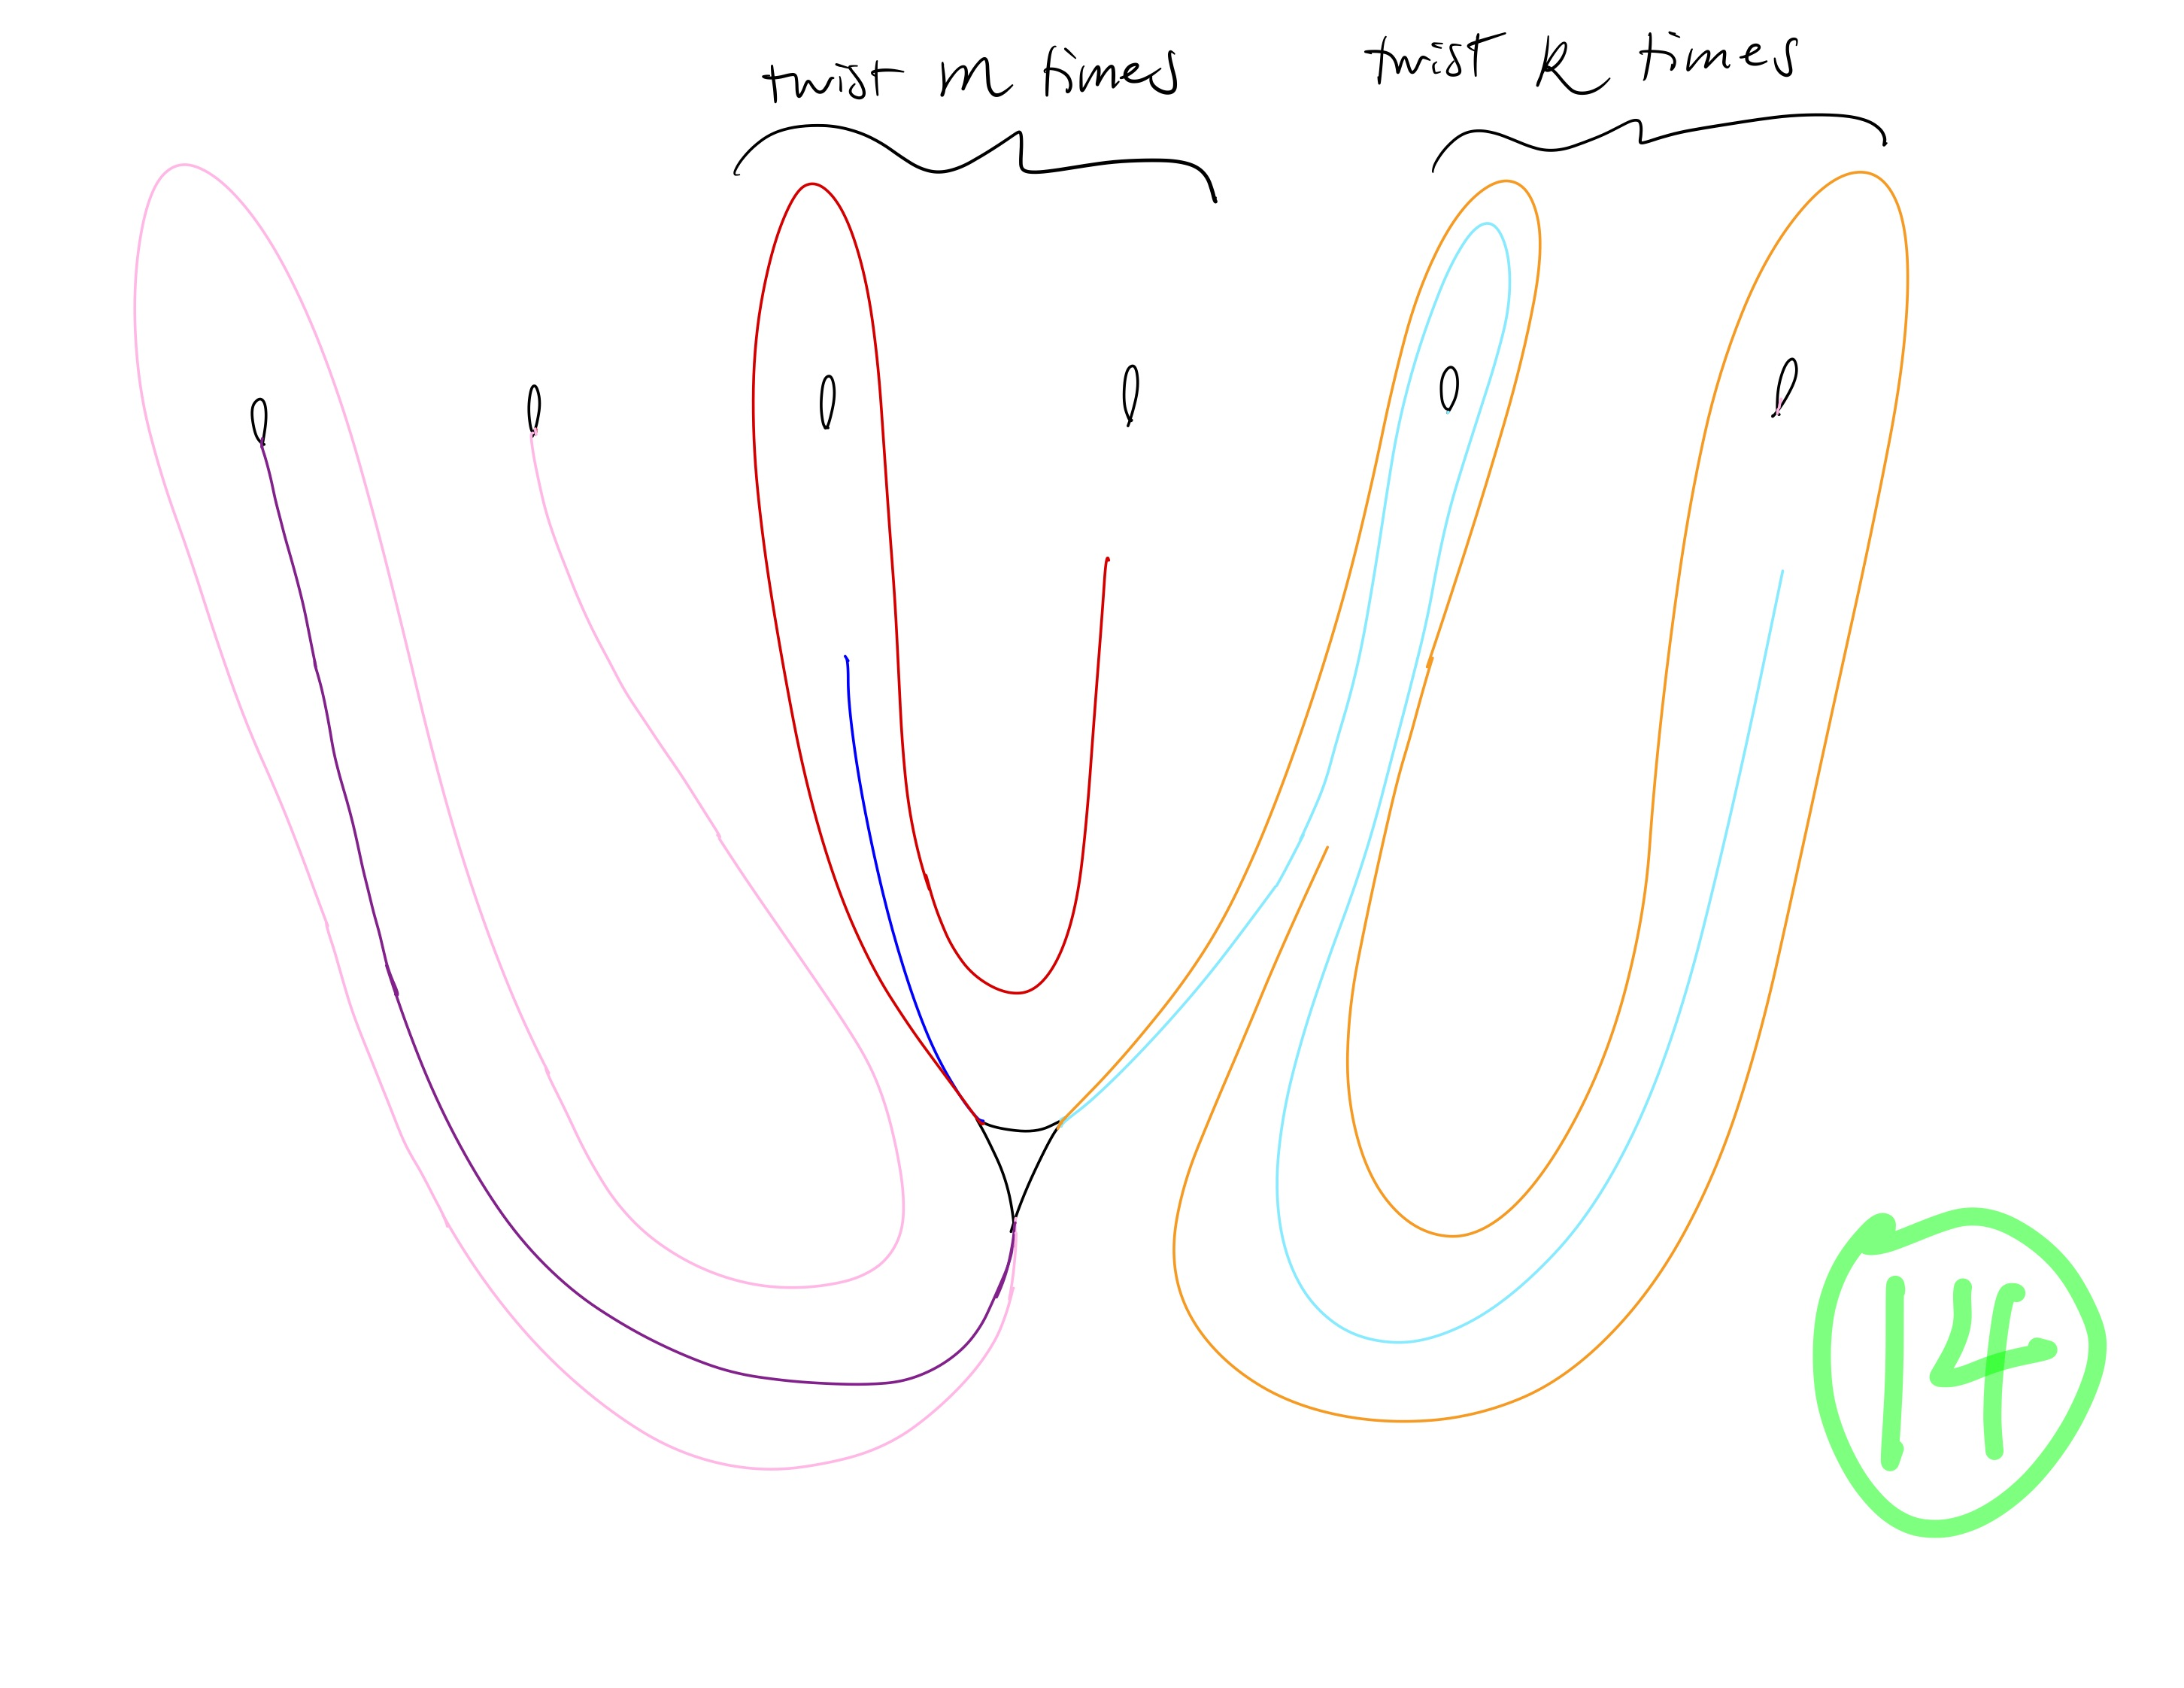
\includegraphics[width=\linewidth, height=0.45\textheight, keepaspectratio]{figures_braid/figures_candelabra/Candelabra Braid 14 Tantivy-1.jpg}
    \caption{Train Track Map Candidate Family 14 of the Candelabra.}
    \label{fig:candelabra_braid_b14_map}
\end{figure*}

The inverse of the following braid carries this family of train track maps:
\[
b_{14}^c = \sigma_{5}^k \sigma_{3}^m \sigma_{1} \sigma_{2} \sigma_{3} \sigma_{4} \circ F \circ G
\]
where $k,m\geq 1$ ($k,m\in \mathbb{Z}$) are the twisting parameters. This is shown in Figure \ref{fig:candelabra_braid_b14}.

\begin{figure*}[p]
    \centering
    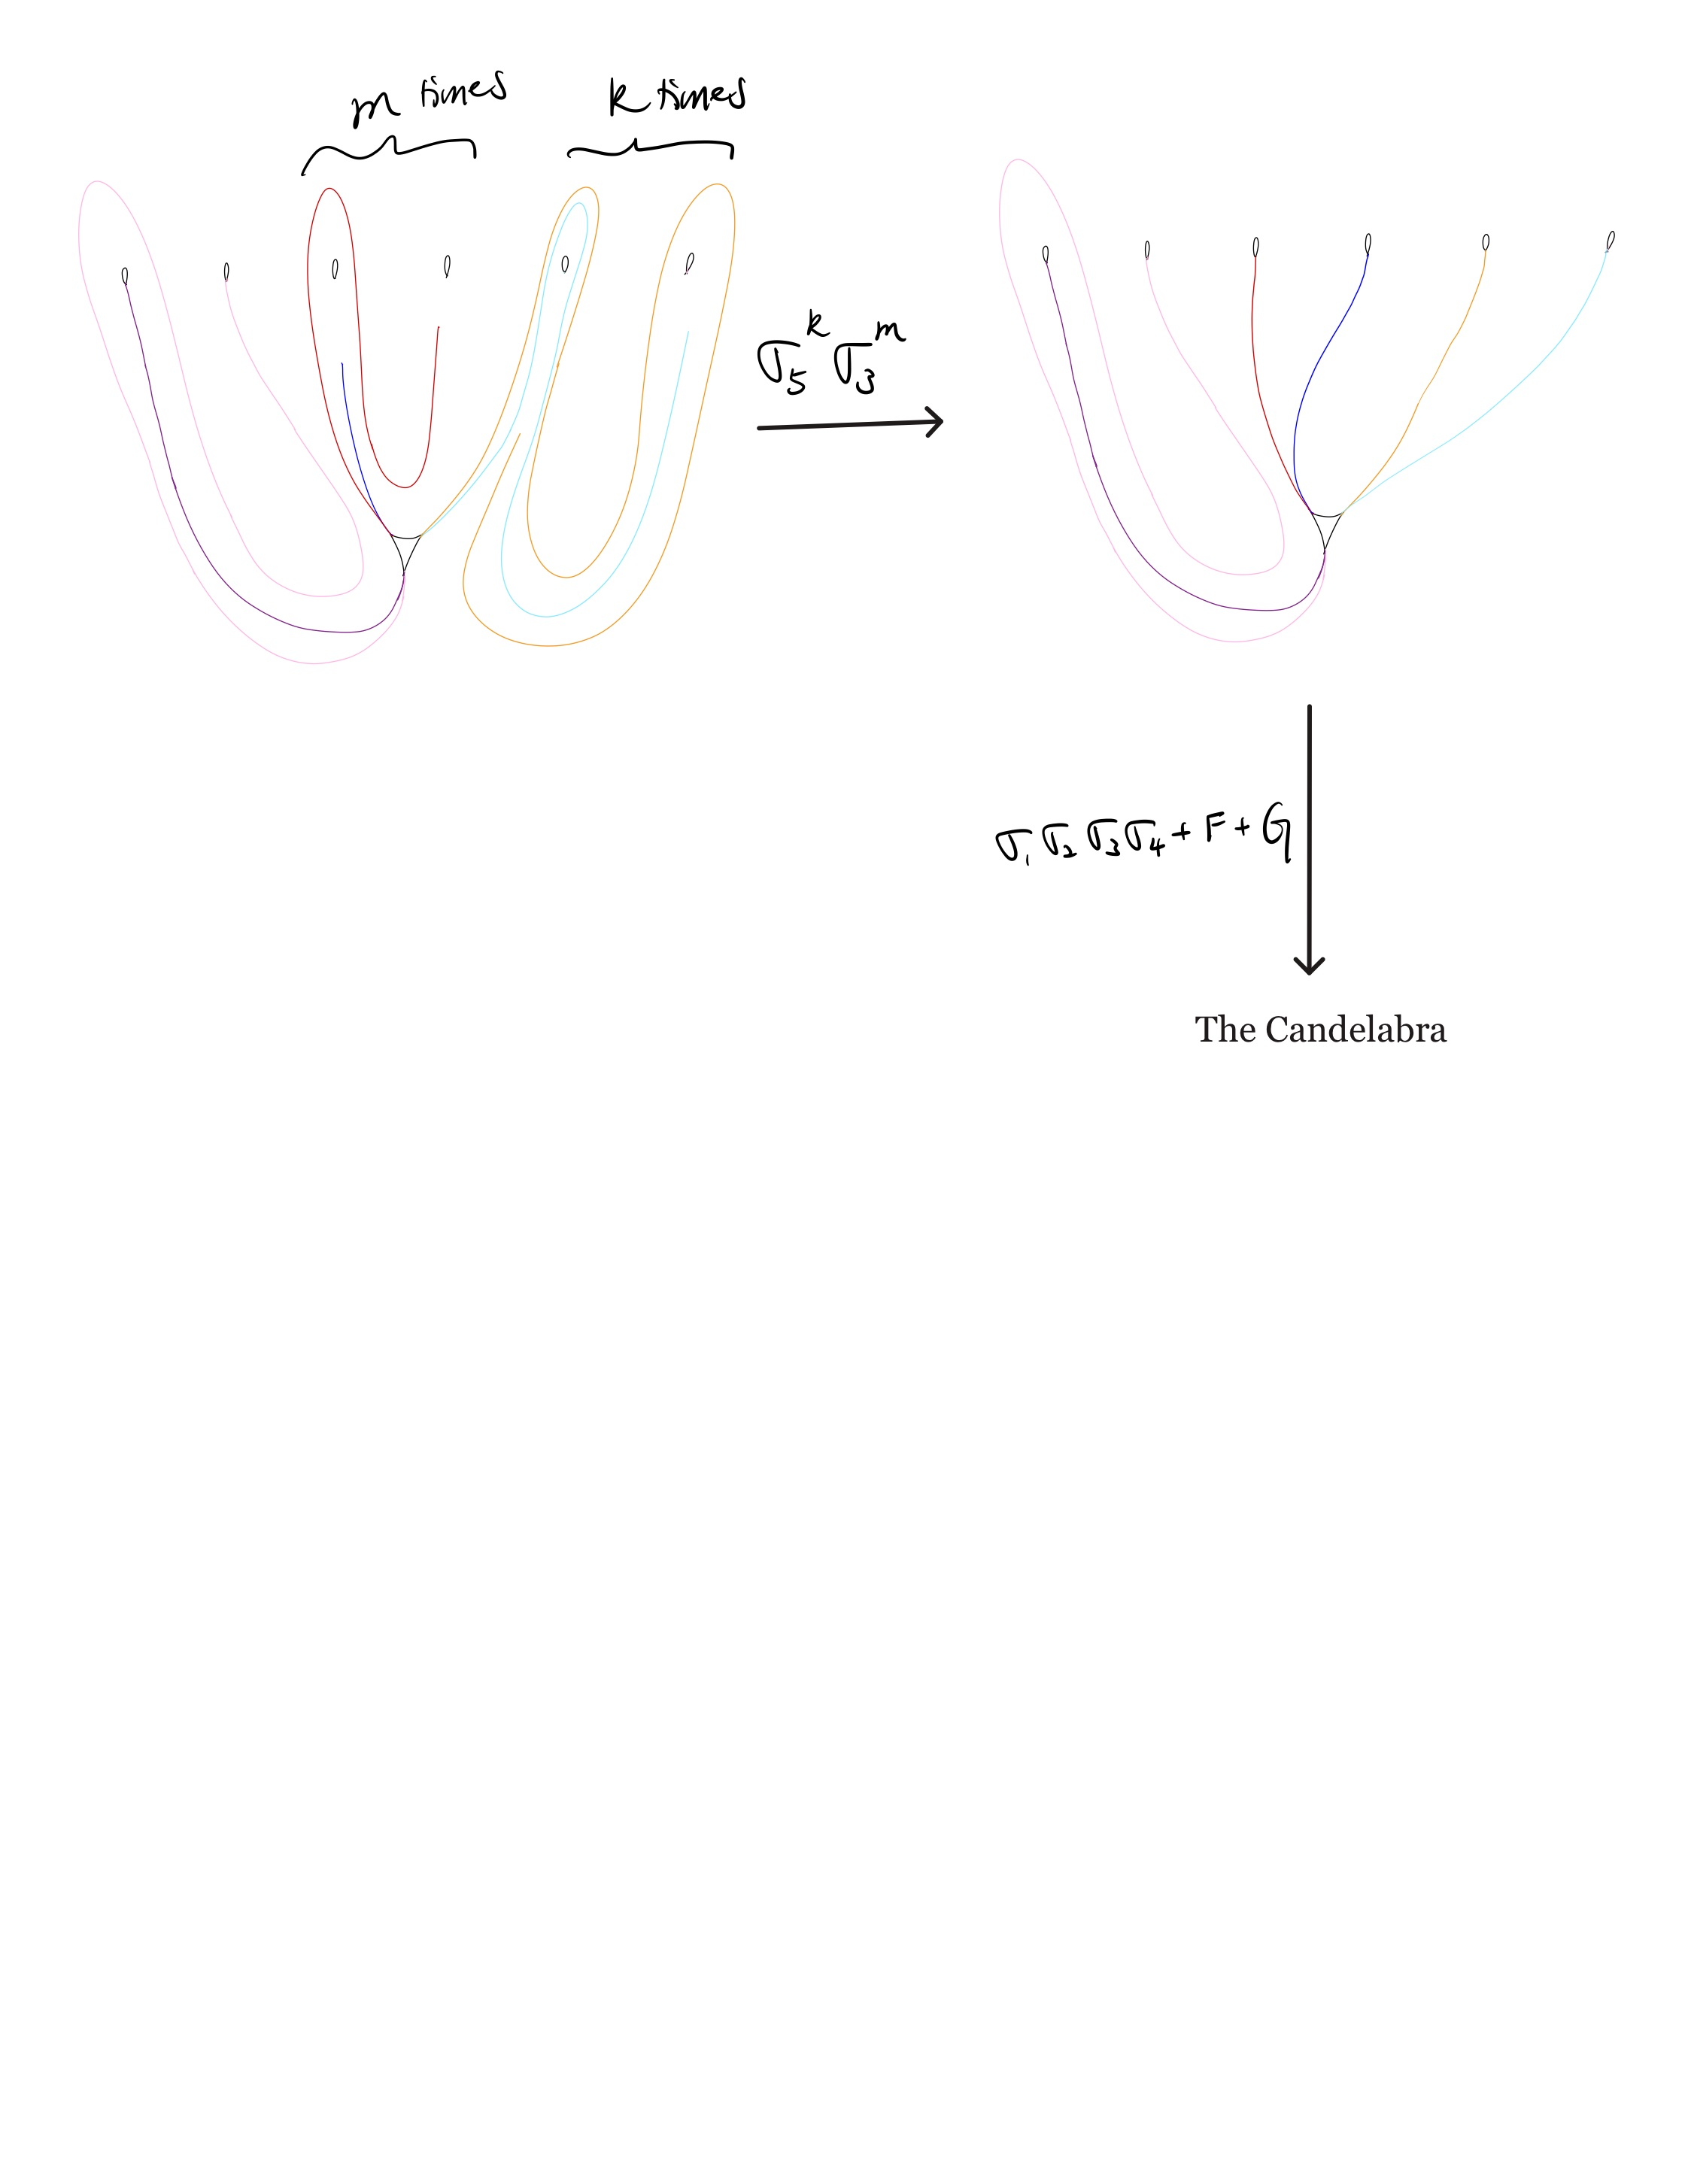
\includegraphics[width=\linewidth, height=0.45\textheight, keepaspectratio]{figures_braid/figures_candelabra/Candelabra Braid 14 Tantivy-2.jpg} 
    \caption{This sequence shows the inverse of the braid $b_{14}^c$ carries Train Track Candidate Family 14.}
    \label{fig:candelabra_braid_b14}
\end{figure*}

\clearpage

\section{Candidate Family 15}
Train Track Map Candidate Family 15 of the Candelabra train track is shown in Figure \ref{fig:candelabra_braid_b15_map}. Note there is twisting between $\fbi$ and $\fbr$. See \ref{Xiphias} for details.

\begin{figure*}[ht]
    \centering
    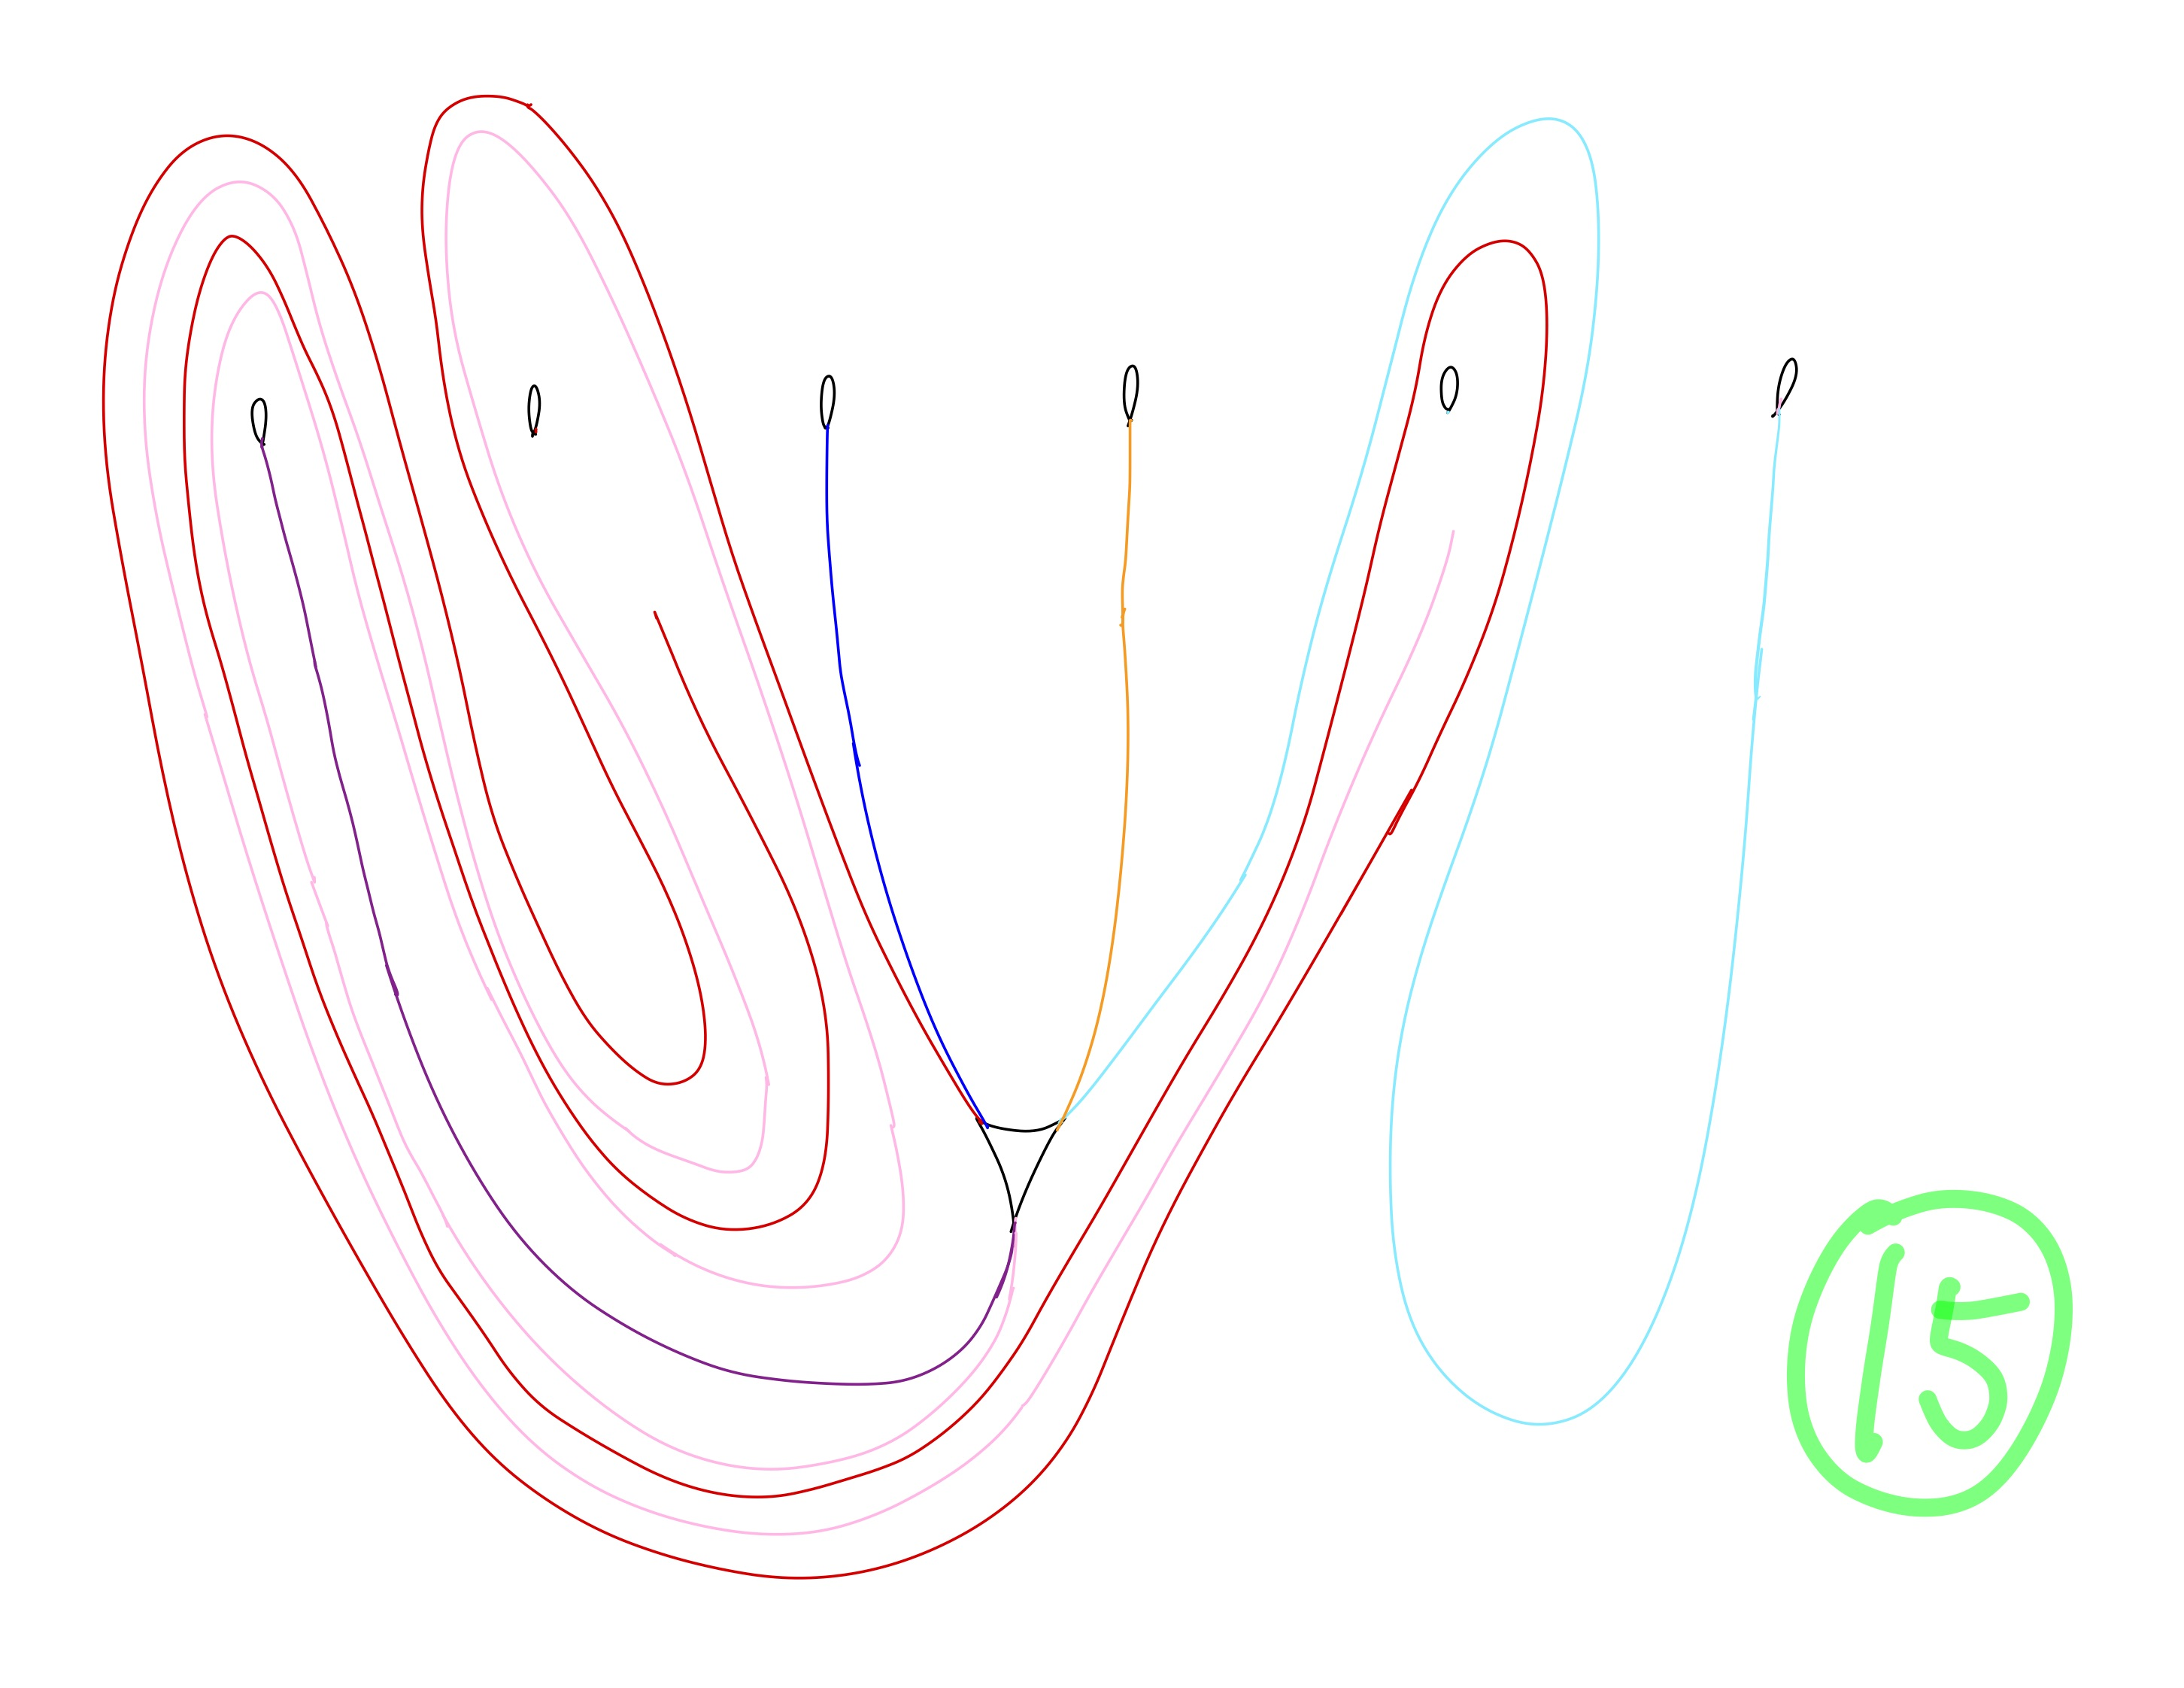
\includegraphics[width=\linewidth, height=0.45\textheight, keepaspectratio]{figures_braid/figures_candelabra/Candelabra Braid 15 Xiphias-1.jpg}
    \caption{Train Track Map Candidate Family 15 of the Candelabra.}
    \label{fig:candelabra_braid_b15_map}
\end{figure*}

The inverse of the following braid carries this family of train track maps:
\[
b_{15}^c = \sigma_{2} \sigma_{1} \sigma_{3} \sigma_{2} \sigma_{5} \sigma_{4} \sigma_{3} \sigma_{4} \sigma_{4} (\sigma_{5}^{-1})^k \sigma_{4}
\]
where $k\geq 1$ ($k\in \mathbb{Z}$) is the twisting parameter. This is shown in Figure \ref{fig:candelabra_braid_b15}.

\begin{figure*}[p]
    \centering
    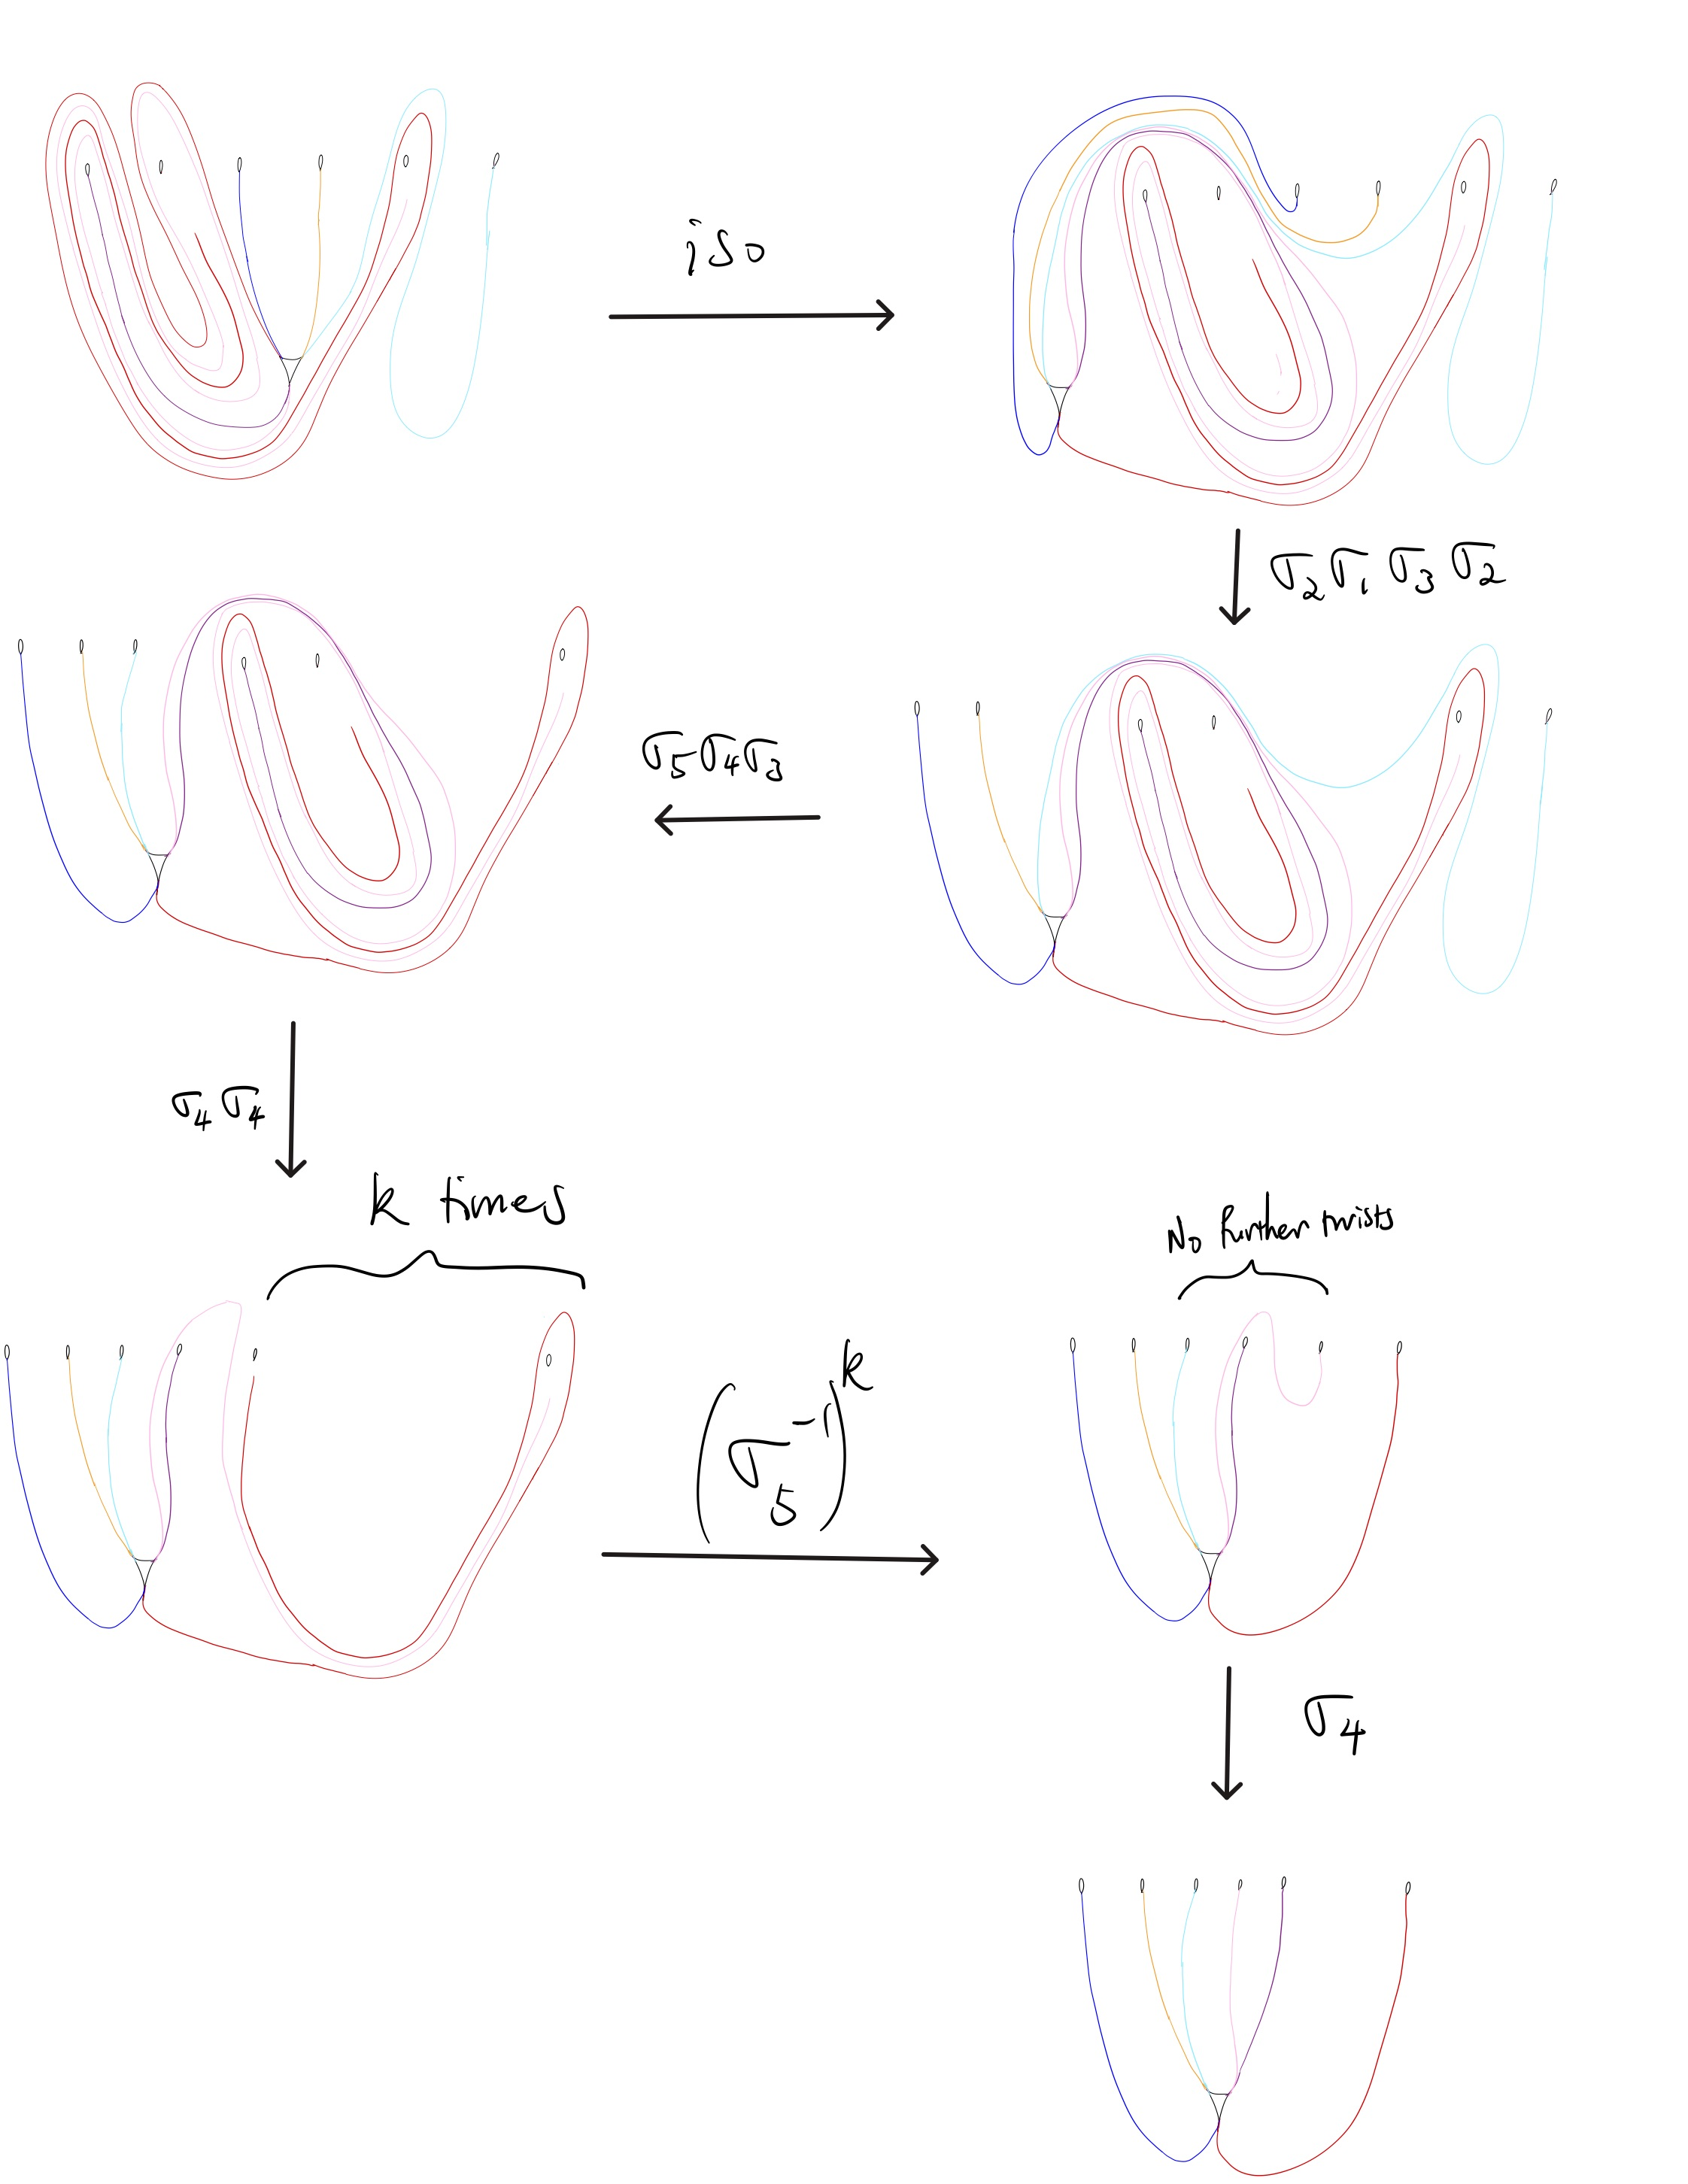
\includegraphics[width=\linewidth, height=0.45\textheight, keepaspectratio]{figures_braid/figures_candelabra/Candelabra Braid 15 Xiphias-2.jpg} 
    \caption{This sequence shows the inverse of the braid $b_{15}^c$ carries Train Track Candidate Family 15.}
    \label{fig:candelabra_braid_b15}
\end{figure*}

\clearpage

\section{Candidate Family 16}
Train Track Map Candidate Family 16 of the Candelabra train track is shown in Figure \ref{fig:candelabra_braid_b16_map}. Note there is twisting between $\fbp$ and $\fbi$; between $\fbr$ and $\fbb$; and between $\fbo$ and $\fbs$. See \ref{Kieve} for details.

\begin{figure*}[ht]
    \centering
    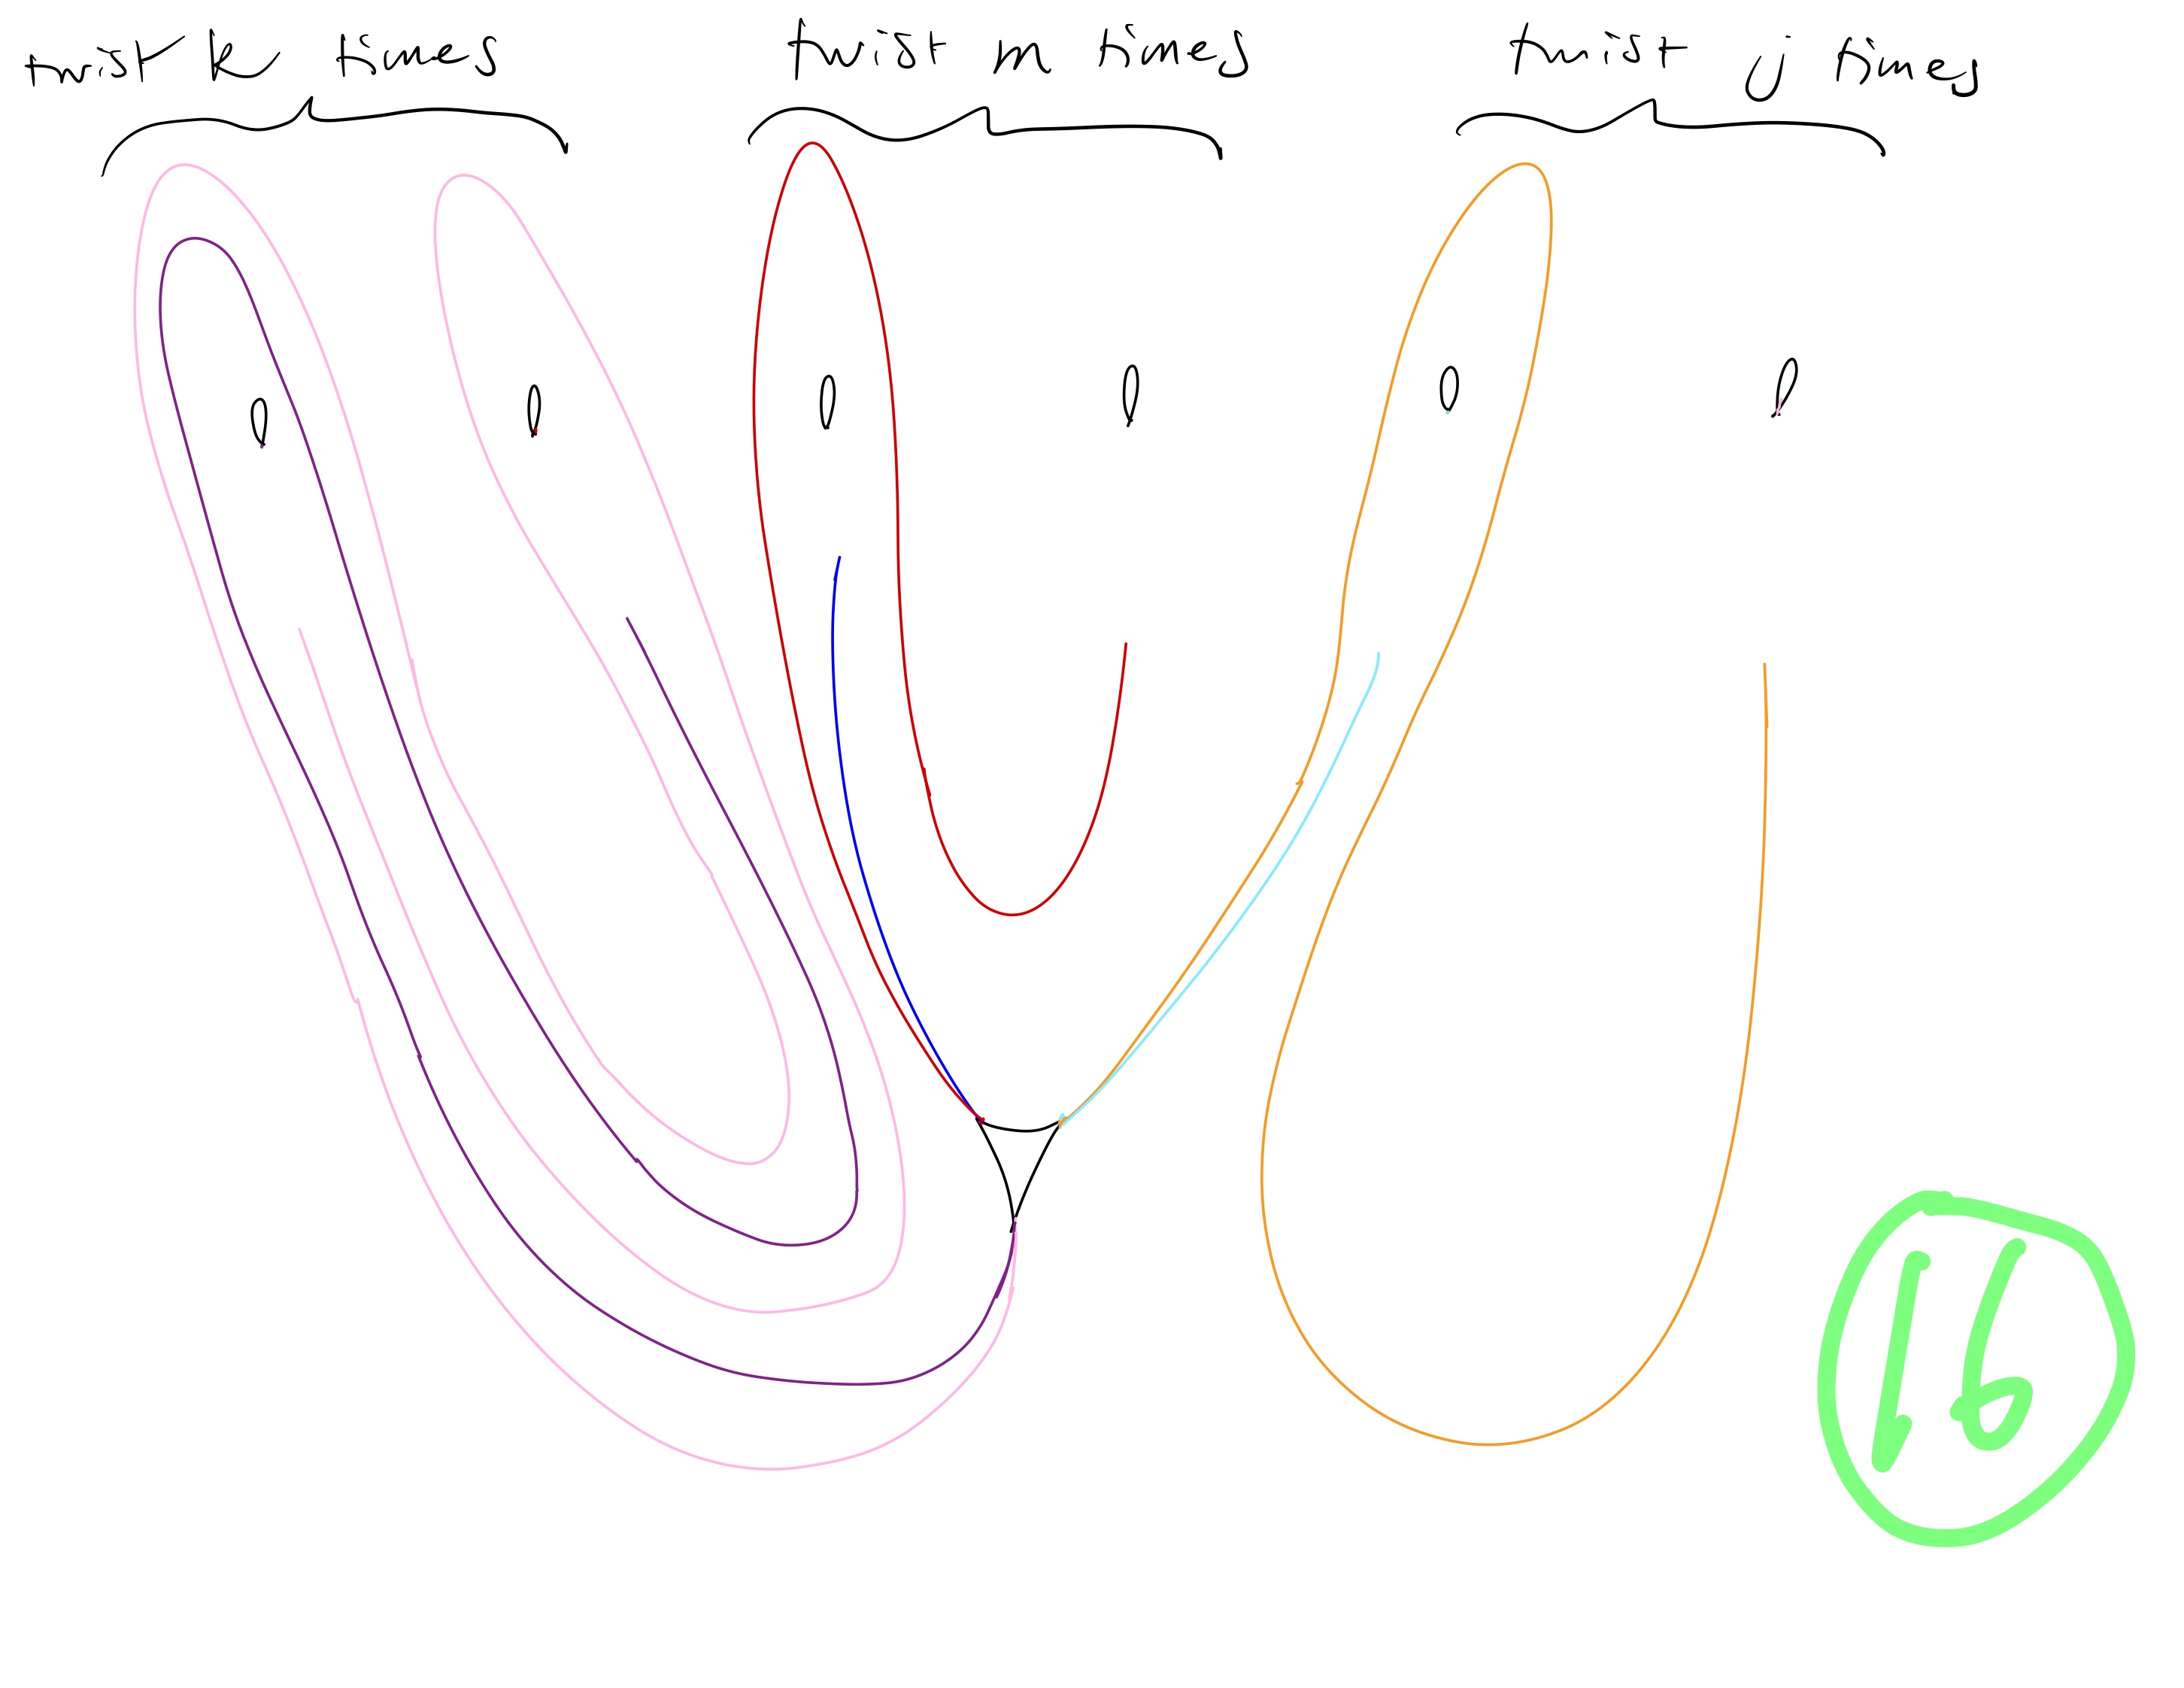
\includegraphics[width=\linewidth, height=0.45\textheight, keepaspectratio]{figures_braid/figures_candelabra/Candelabra Braid 16 Kieve-1.jpg}
    \caption{Train Track Map Candidate Family 16 of the Candelabra.}
    \label{fig:candelabra_braid_b16_map}
\end{figure*}

The inverse of the following braid carries this family of train track maps:
\[
b_{16}^c = \sigma_{5}^j \sigma_{3}^m \sigma_{1}^k \circ H \circ G
\]
where $k,m,j\geq 1$ ($k,m,j\in \mathbb{Z}$) are the twisting parameters. This is shown in Figure \ref{fig:candelabra_braid_b16}.

\begin{figure*}[p]
    \centering
    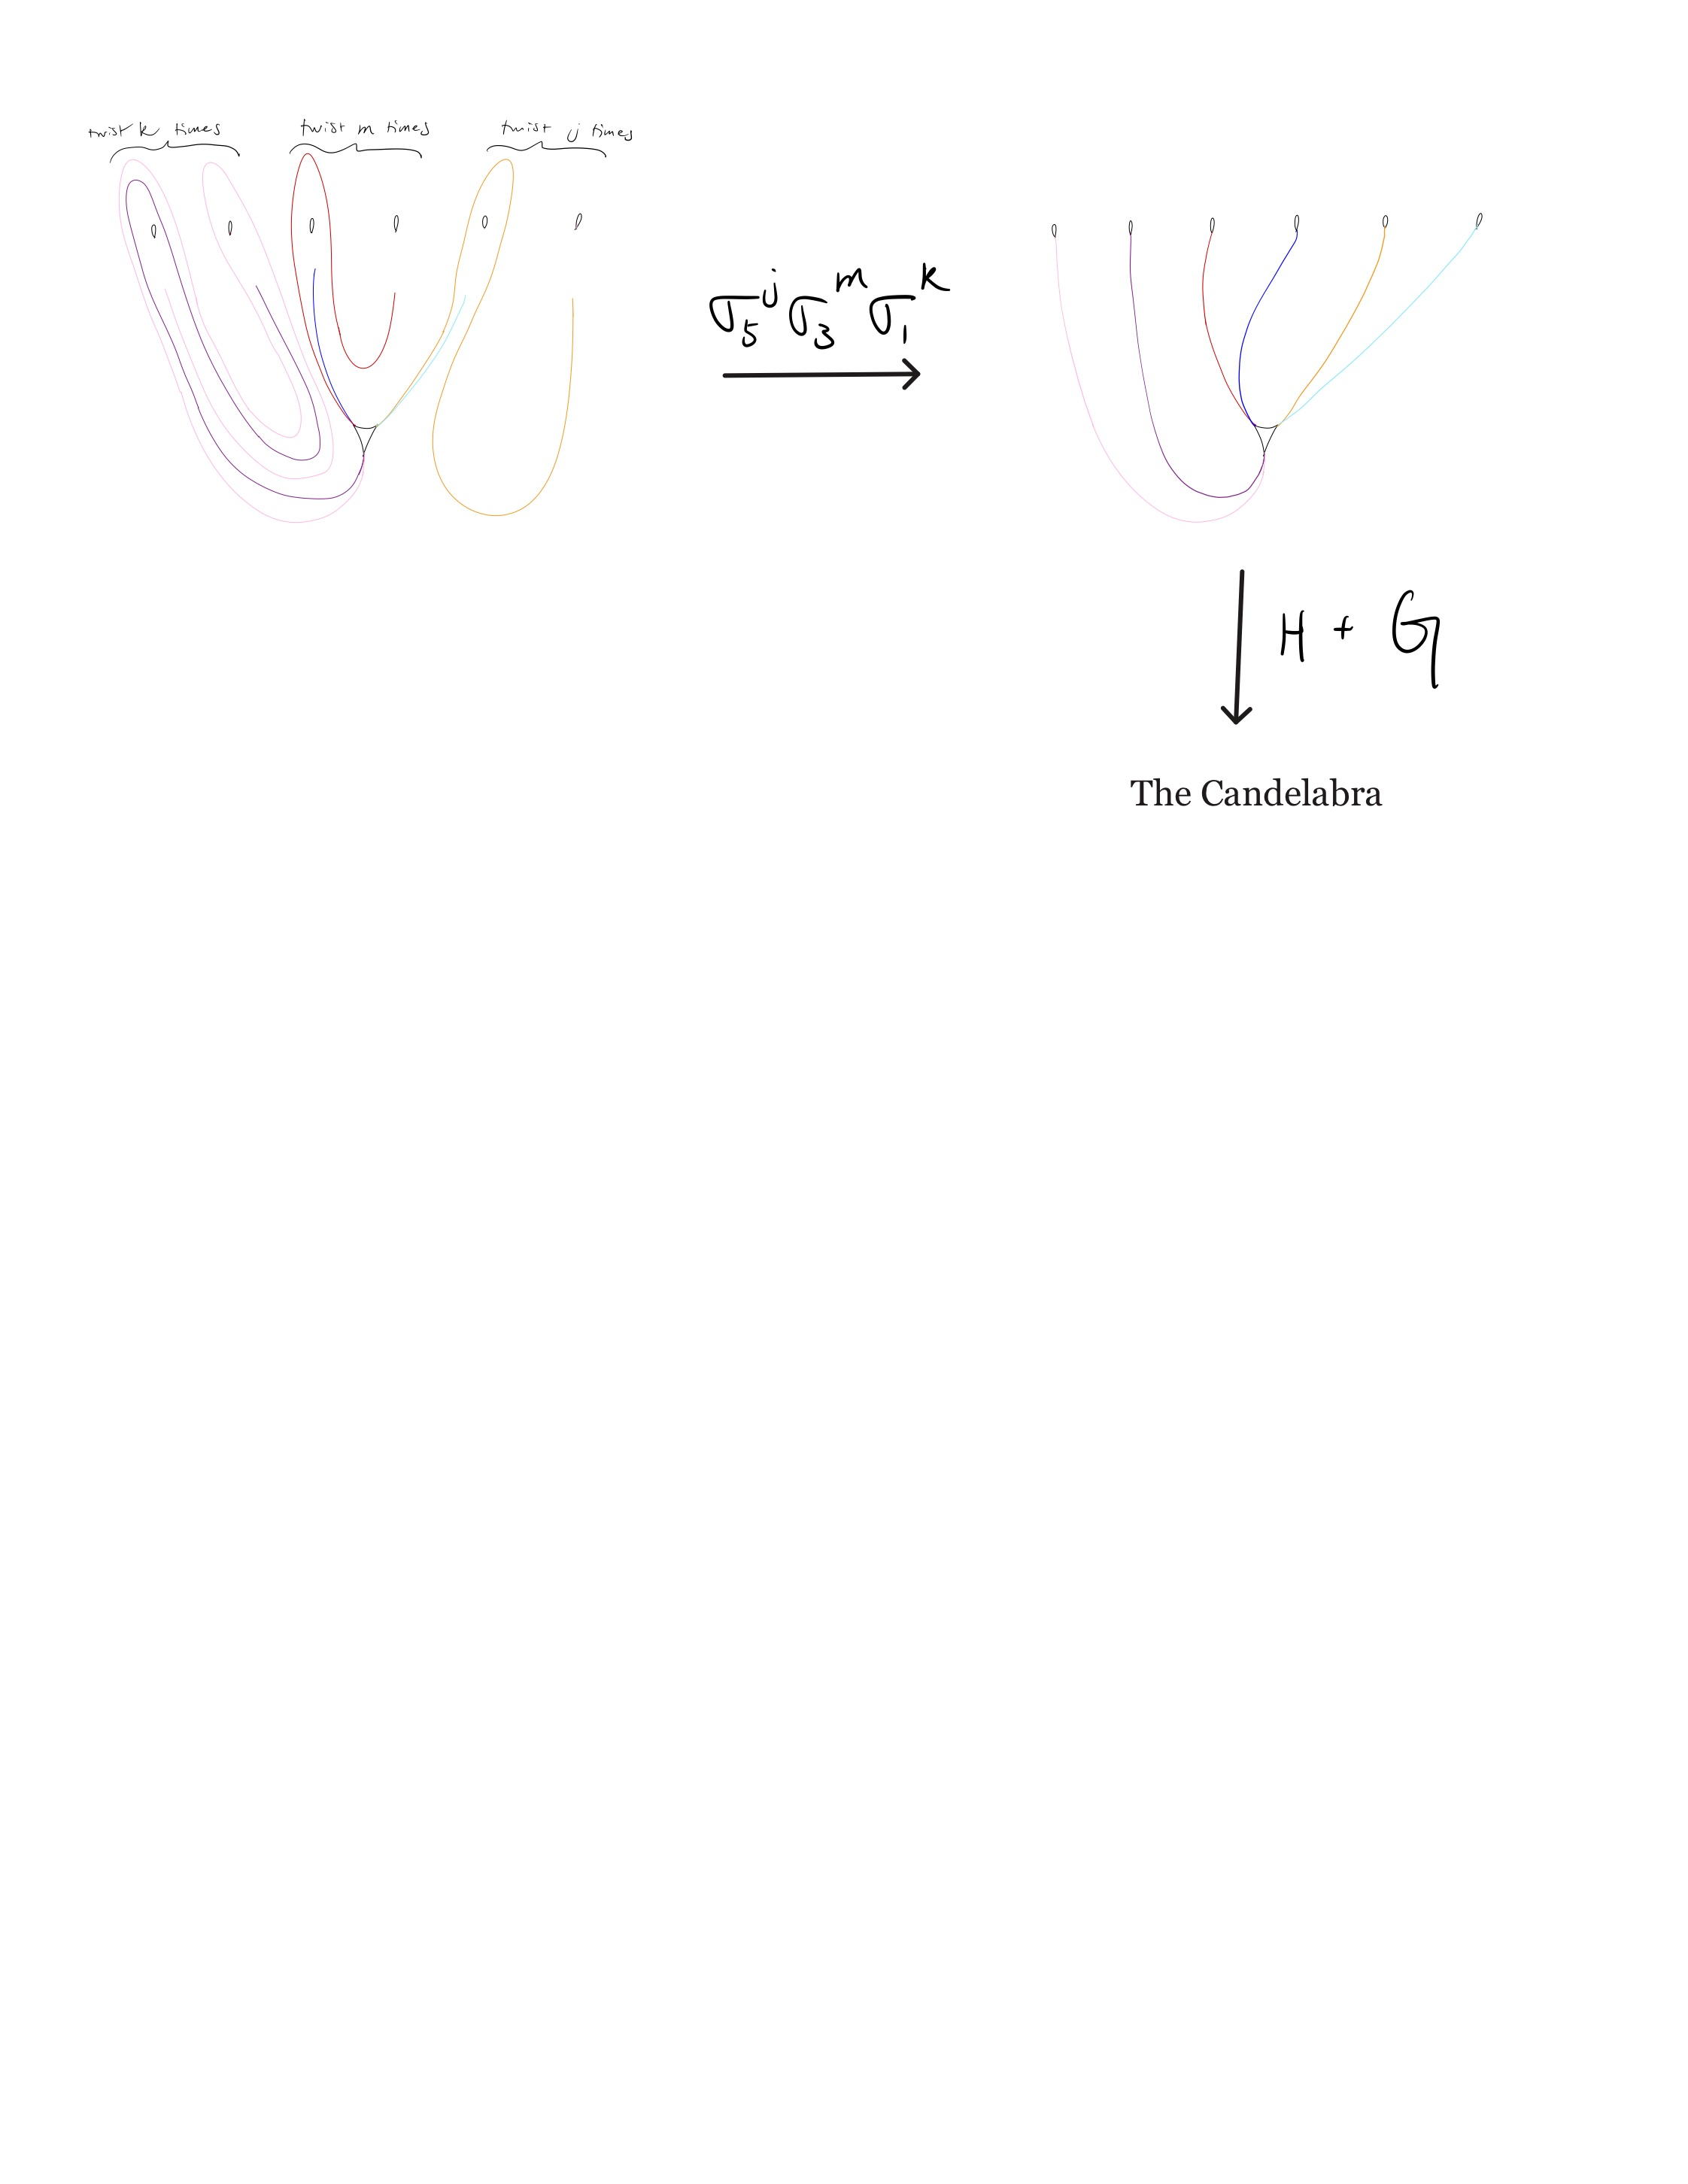
\includegraphics[width=\linewidth, height=0.45\textheight, keepaspectratio]{figures_braid/figures_candelabra/Candelabra Braid 16 Kieve-2.jpg}\\
    \includegraphics[width=\linewidth, height=0.45\textheight, keepaspectratio]{figures_braid/figures_candelabra/Candelabra Braid 16 Kieve-3.jpg}
    \caption{This sequence shows the inverse of the braid $b_{16}^c$ carries Train Track Candidate Family 16.}
    \label{fig:candelabra_braid_b16}
\end{figure*}

\clearpage

\section{Candidate Family 17}
Train Track Map Candidate Family 17 of the Candelabra train track is shown in Figure \ref{fig:candelabra_braid_b17_map}. Note there is twisting among $\fbi$, $\fbp$, and $\fbr$. See \ref{Oorie} for details.

\begin{figure*}[ht]
    \centering
    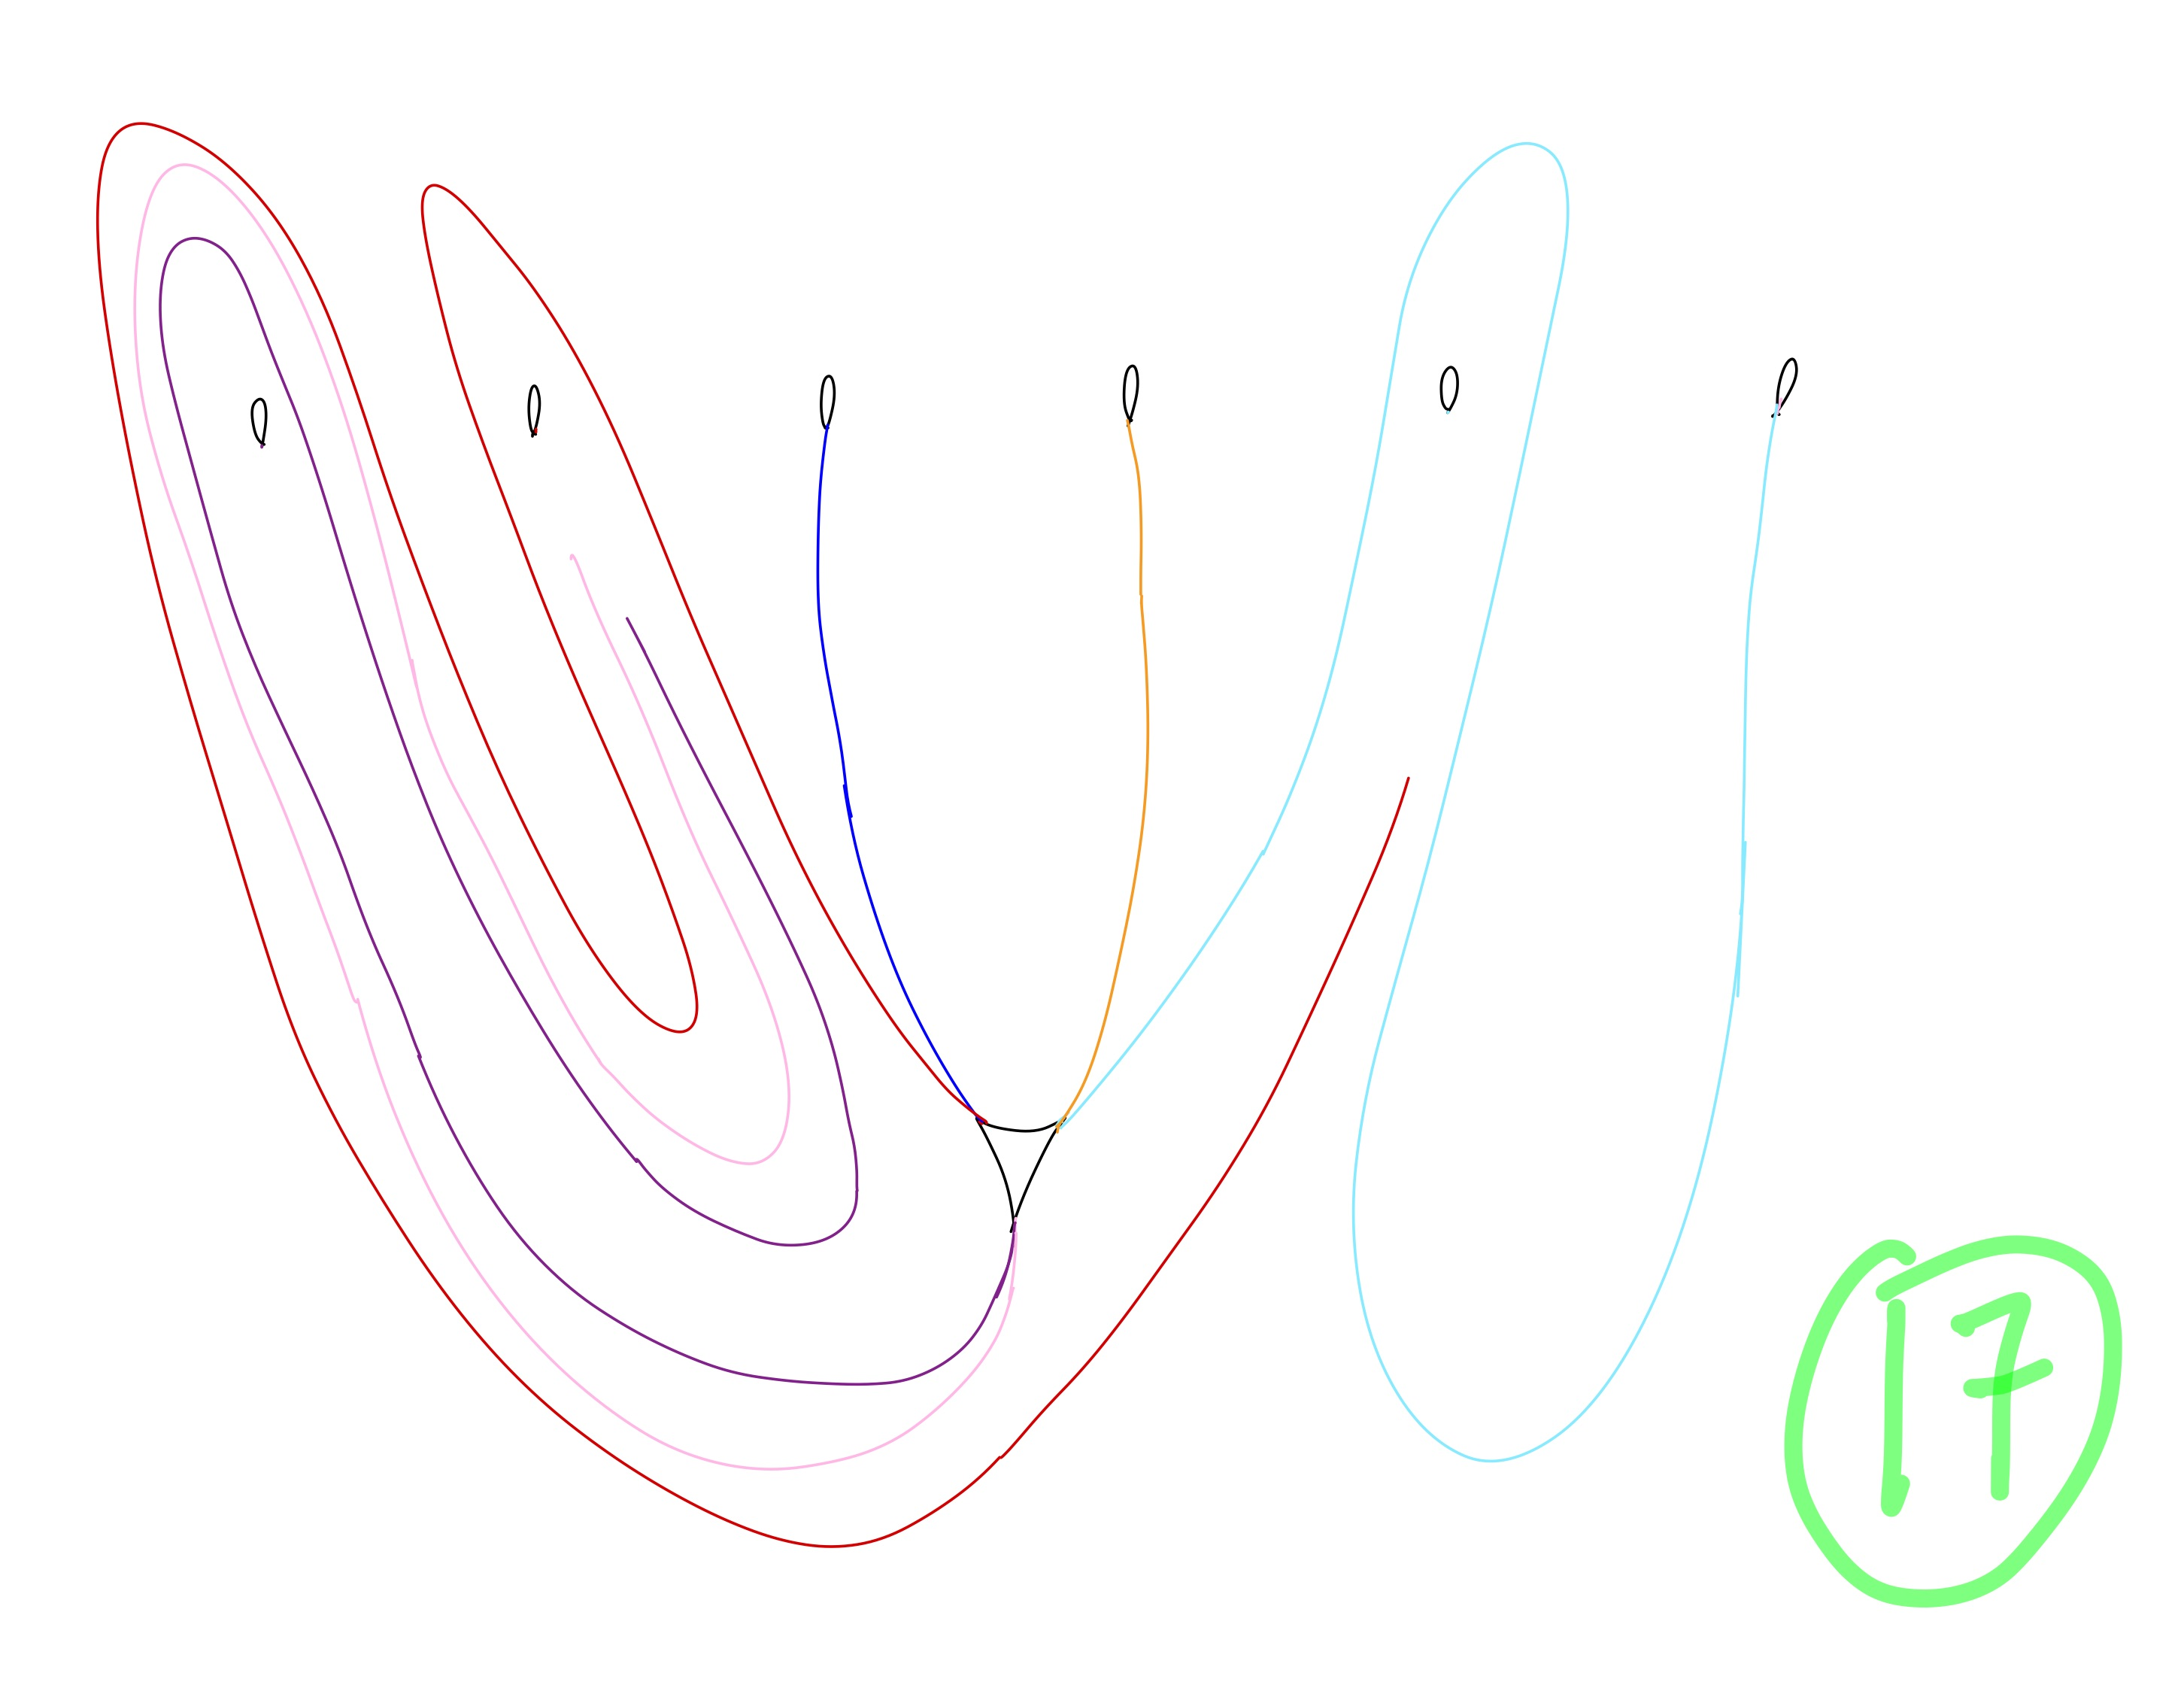
\includegraphics[width=\linewidth, height=0.45\textheight, keepaspectratio]{figures_braid/figures_candelabra/Candelabra Braid 17 Oorie-1.jpg}
    \caption{Train Track Map Candidate Family 17 of the Candelabra.}
    \label{fig:candelabra_braid_b17_map}
\end{figure*}

The inverse of the following braid carries this family of train track maps:
\[
b_{17}^c = \sigma_{1}^k \sigma_{2} \sigma_{1} \sigma_{5} \sigma_{4} \sigma_{3} \sigma_{2} \sigma_{4} \sigma_{3} \sigma_{4} (\sigma_{5}^{-1})^m \sigma_{4}
\]
where $k,m\geq 1$ ($k,m\in \mathbb{Z}$) are the twisting parameters. This is shown in Figure \ref{fig:candelabra_braid_b17}.

\begin{figure*}[p]
    \centering
    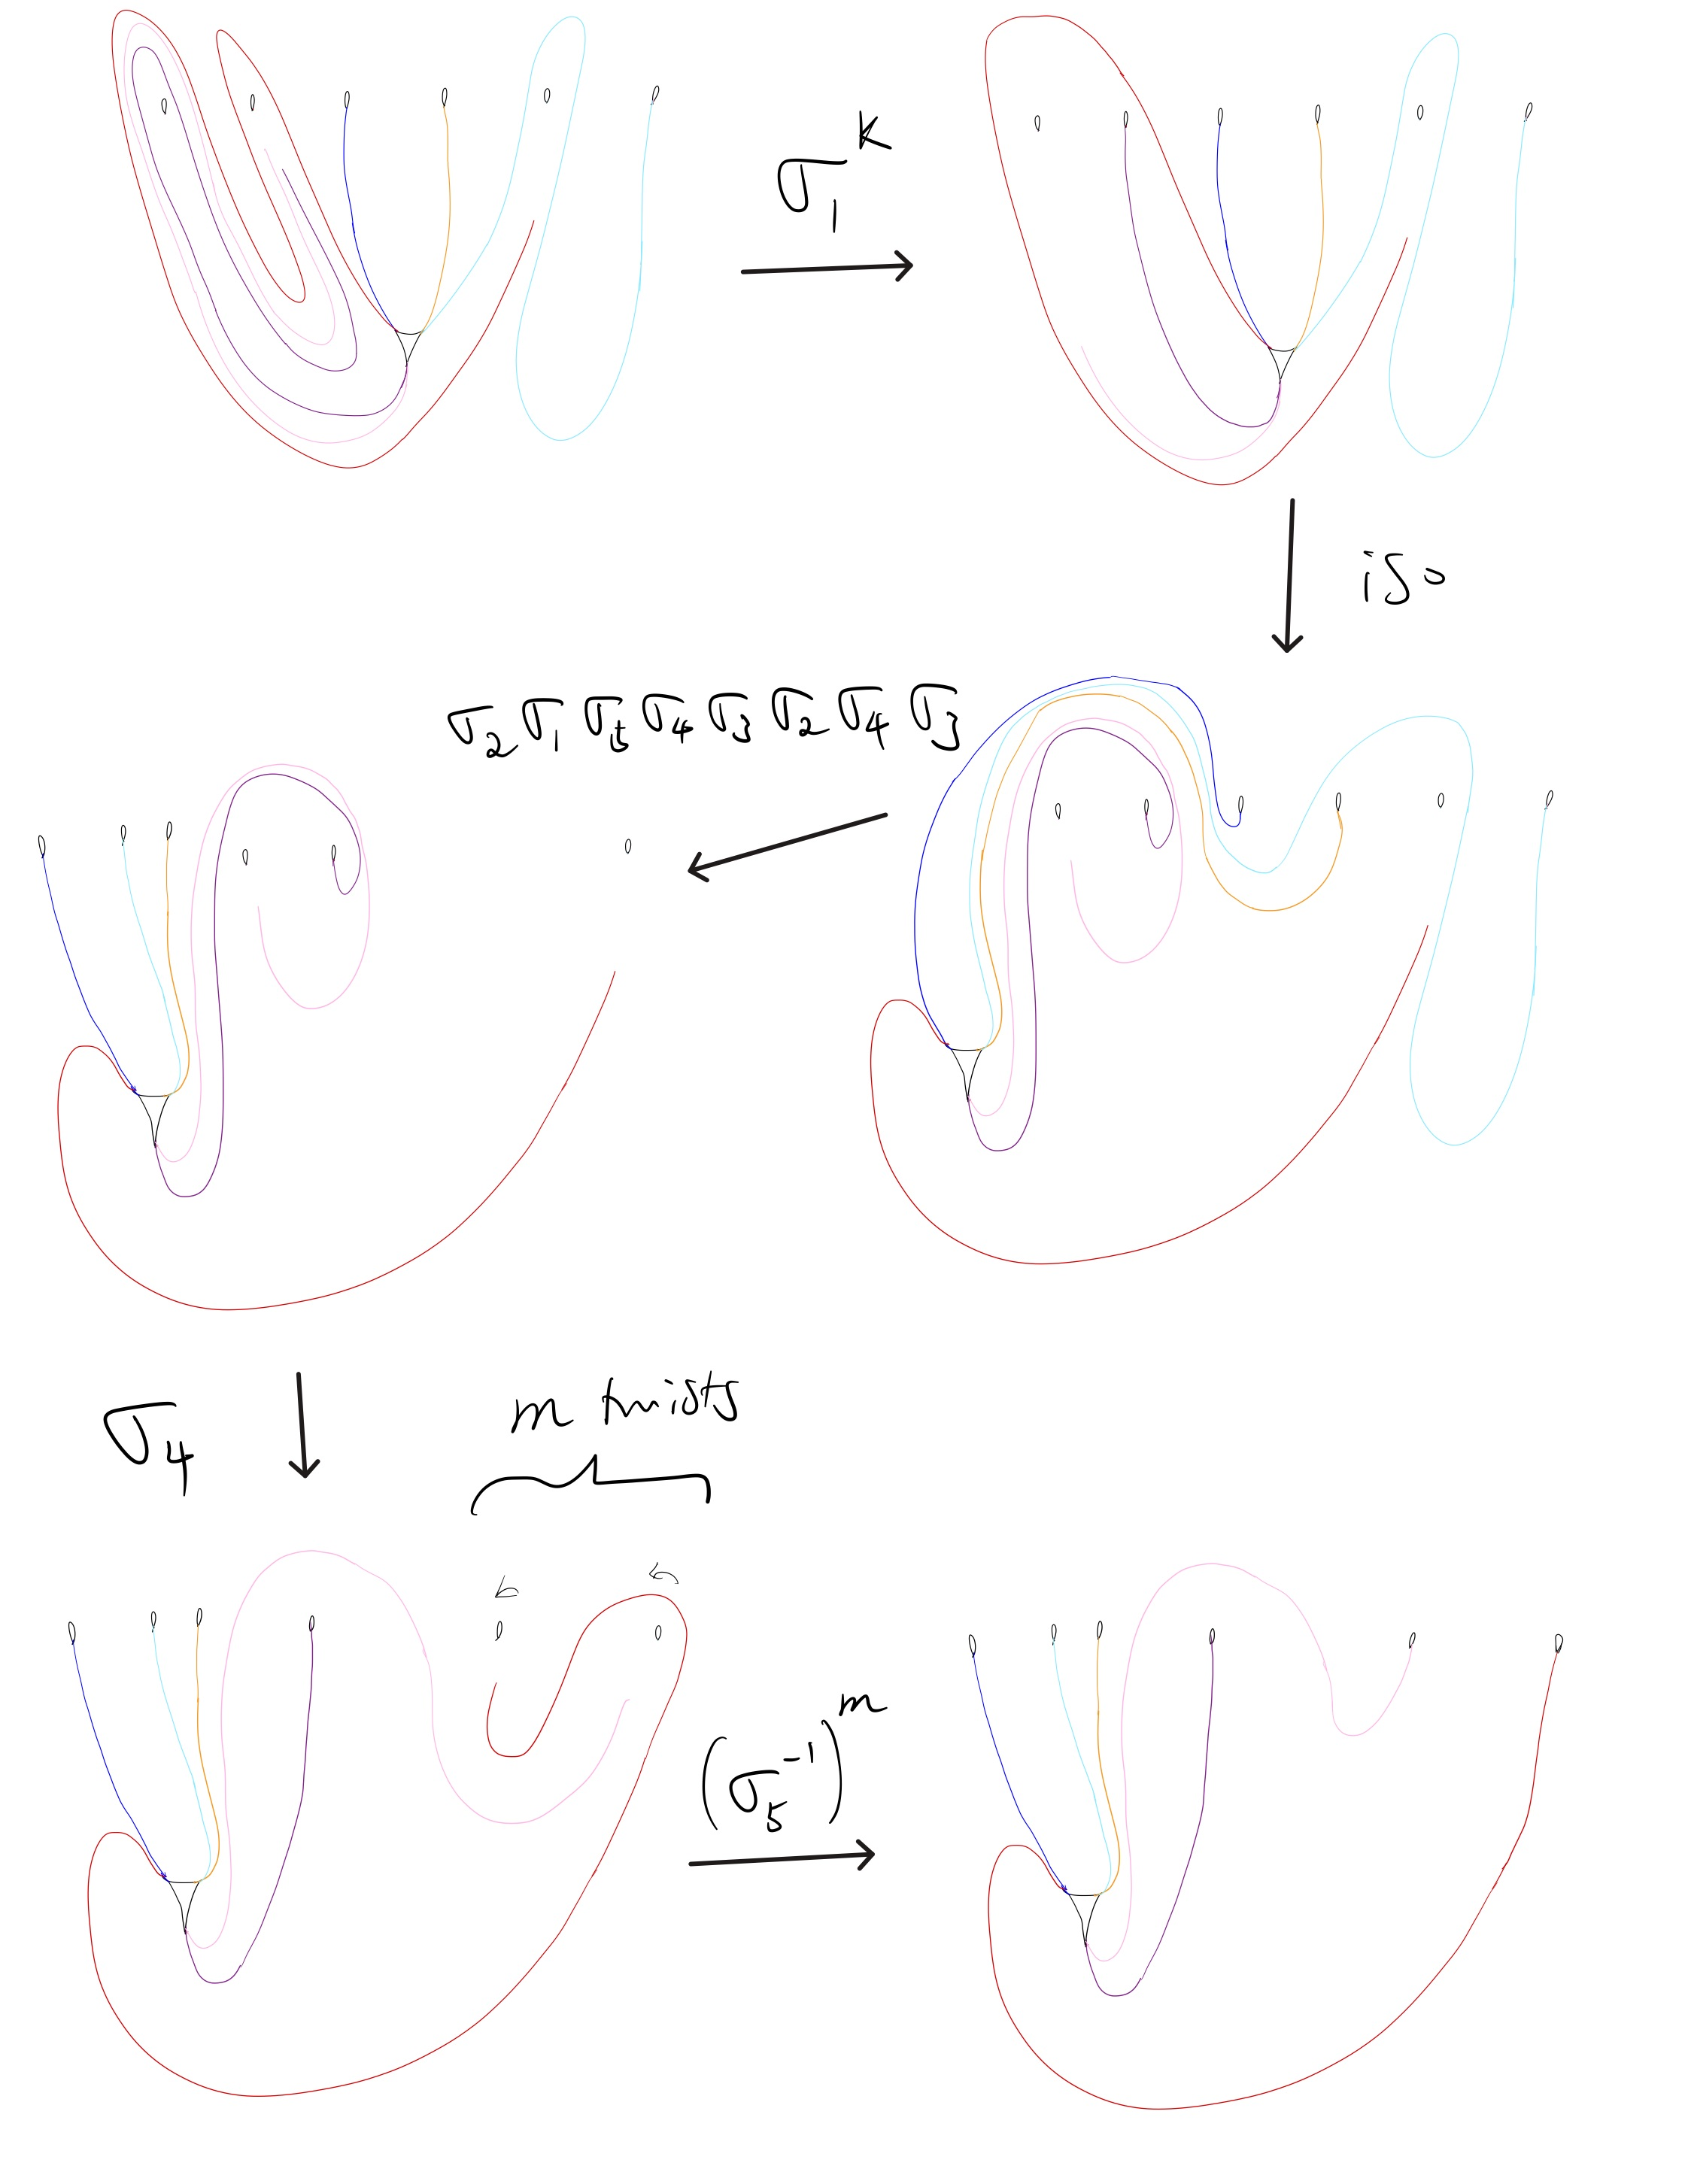
\includegraphics[width=\linewidth, height=0.45\textheight, keepaspectratio]{figures_braid/figures_candelabra/Candelabra Braid 17 Oorie-2.jpg}\\
    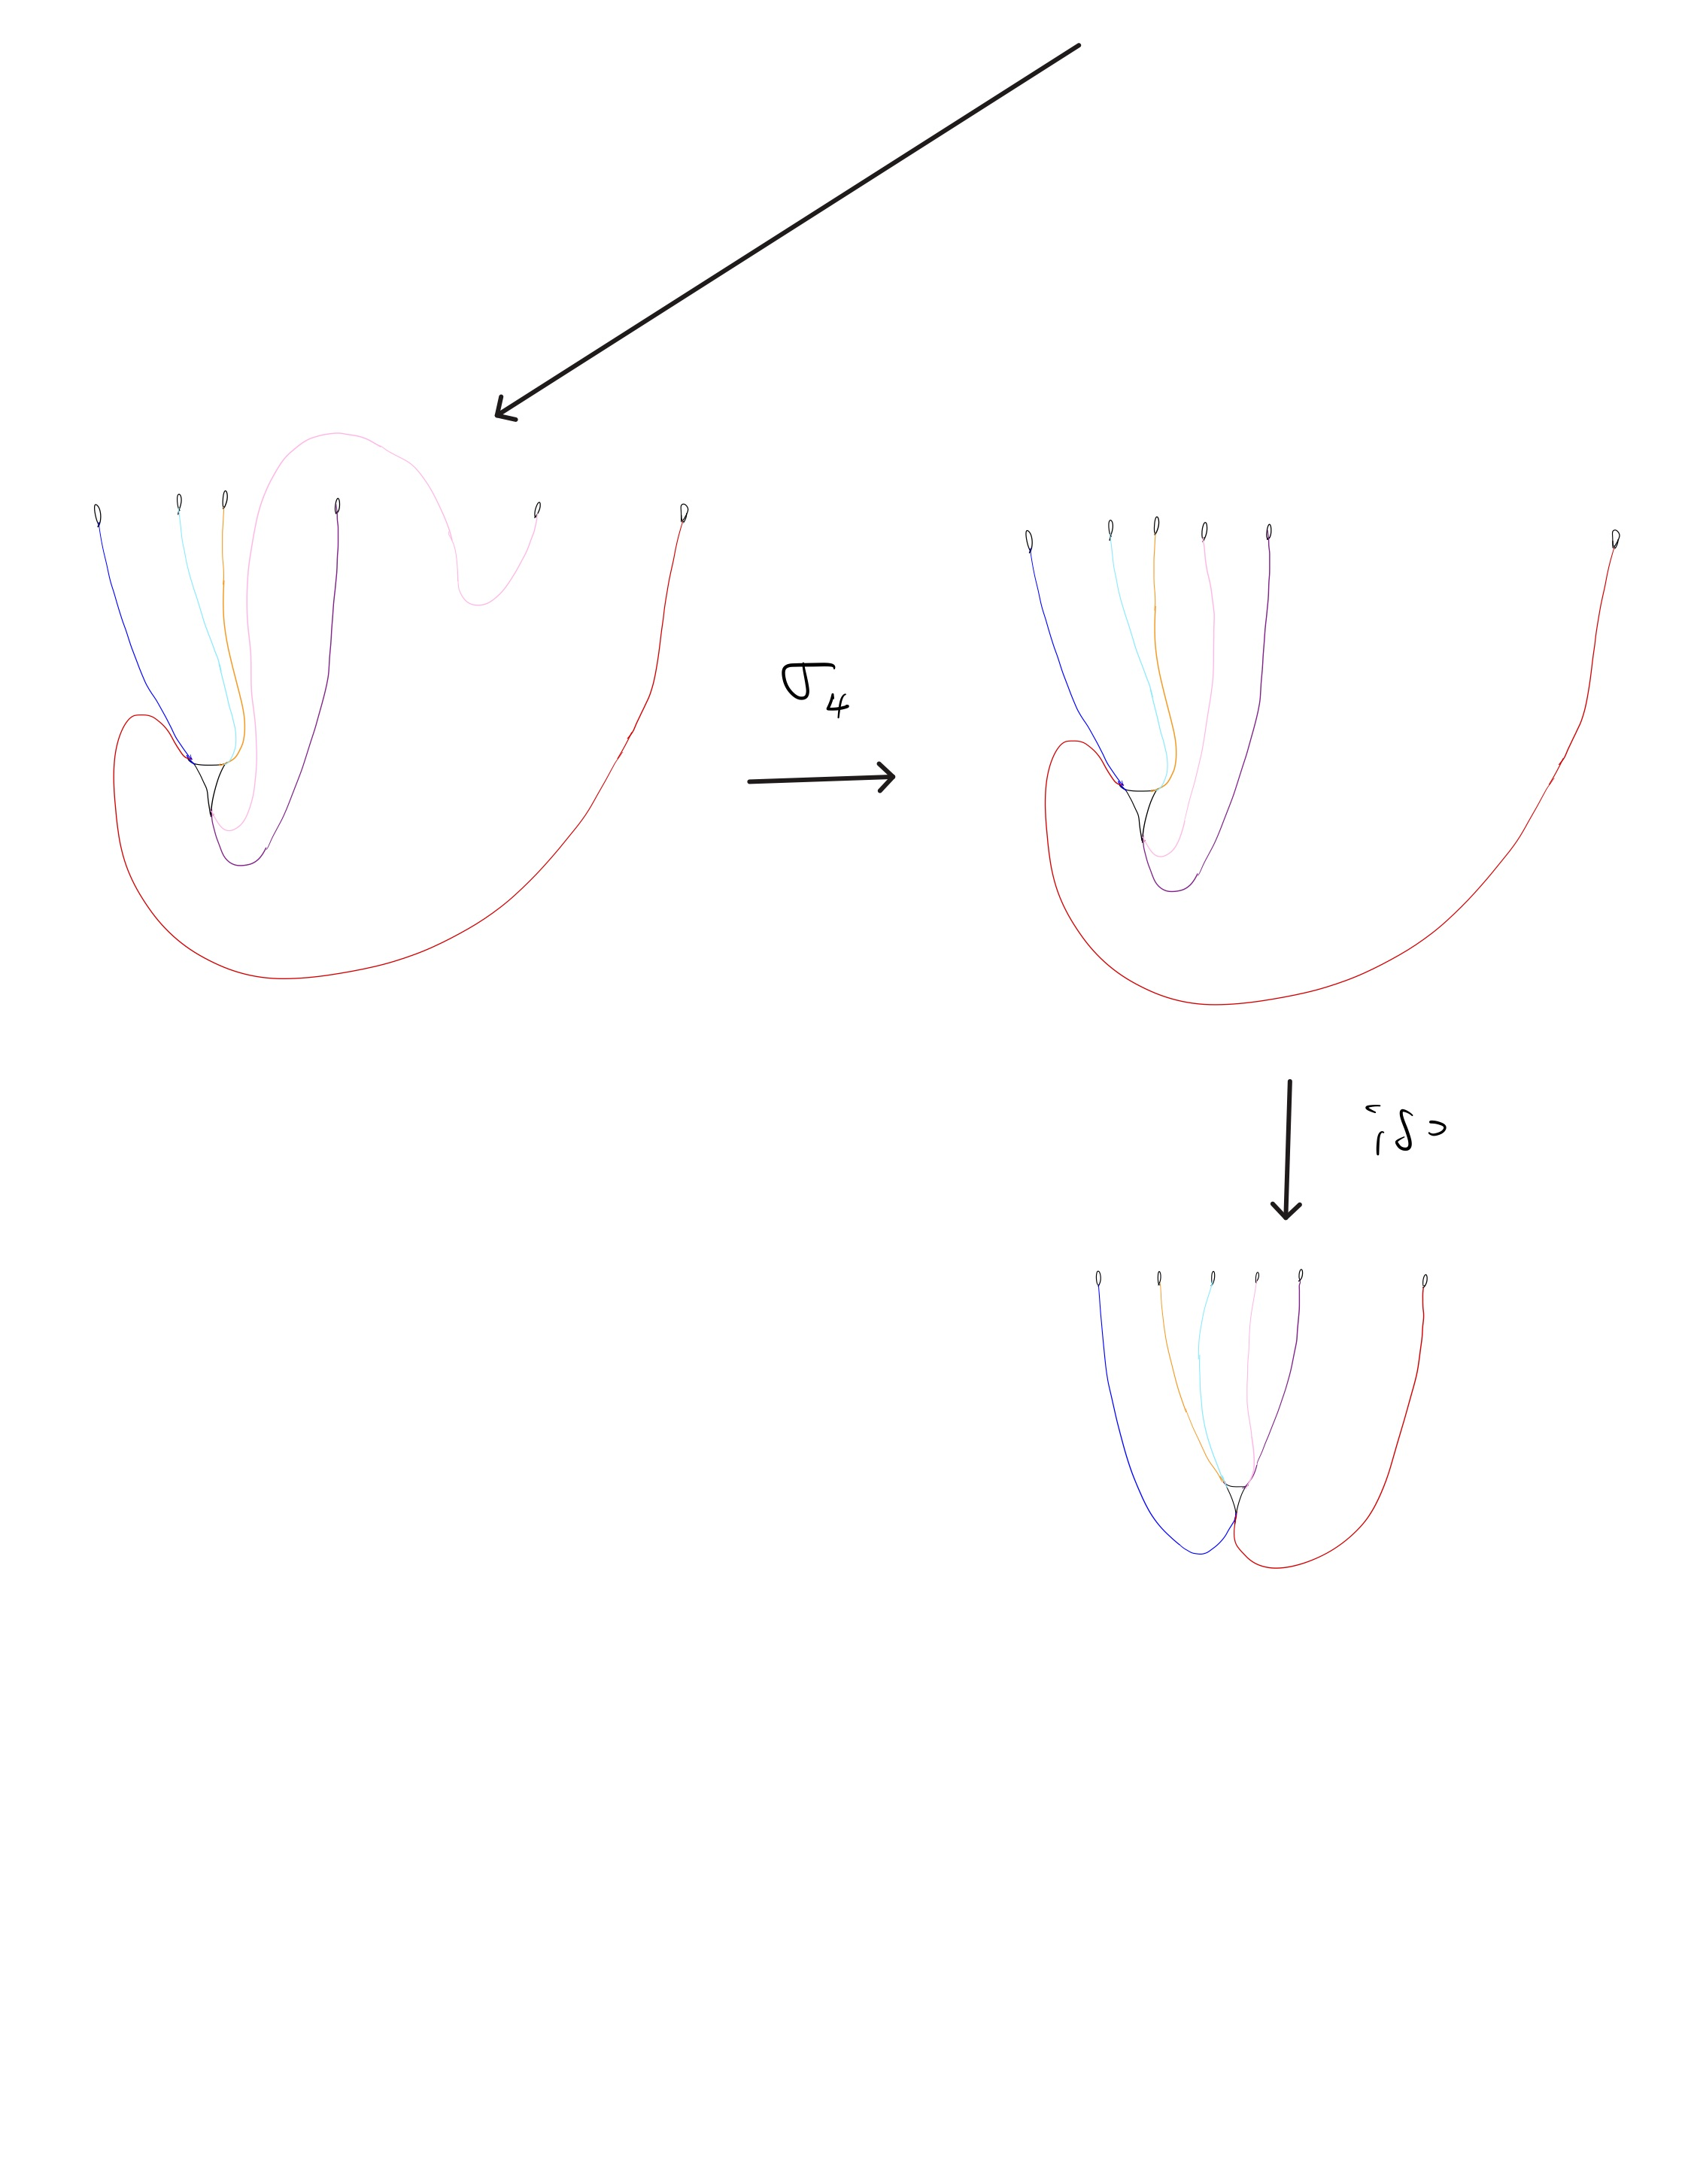
\includegraphics[width=\linewidth, height=0.45\textheight, keepaspectratio]{figures_braid/figures_candelabra/Candelabra Braid 17 Oorie-3.jpg} 
    \caption{This sequence shows the inverse of the braid $b_{17}^c$ carries Train Track Candidate Family 17.}
    \label{fig:candelabra_braid_b17}
\end{figure*}